
\documentclass[12pt]{report}
%%%\usefpackage[cp866]{inputenc}
%%%\usepackage[koi8-r]{inputenc}
%%%\usepackage[russian]{babel}
\usepackage{rotating}
\usepackage[usenames]{color}
%\usepackage{epsfig}
\usepackage{overpic}
\usepackage{url}
\usepackage{pst-plot}
\usepackage{amsmath,fullpage,graphicx,caption,float}
\usepackage{amssymb}
\usepackage{array,ragged2e,pst-node,pst-dbicons}
\usepackage{pstricks}
\usepackage{pst-node}
\usepackage{pst-blur}
\usepackage{comment}
\usepackage{color}
\usepackage{subfigure}
\usepackage{lscape}
\usepackage{multirow}
%\usepackage{hyperref}
\usepackage{mathtools}
\usepackage{framed}
\usepackage{diagbox}

\newcommand{\defeq}{\vcentcolon=}

\usepackage{float}
\restylefloat{table}
\usepackage[margin=20mm]{geometry}

\setlength{\parskip}{1.25ex}
\renewcommand\baselinestretch{1.3}
\renewcommand\arraystretch{1.5}

% equation numbering:
\numberwithin{equation}{section}

\mathchardef\mhyphen="2D
\definecolor{Pink}{rgb}{1.,0.75,0.8}
\newcolumntype{C}[1]{>{\Centering}p{#1}}
\def\Tab#1{\tabular{C{3cm}}\rule[-5mm]{0pt}{1cm}#1\\\hline
                           ~\\\hline~\endtabular}
\seticonparams{entity}{shadow,fillcolor=black!20,fillstyle=solid,framesep=0pt}

\mathchardef\mhyphen="2D
\usepackage[numbers,sort&compress]{natbib}
\usepackage[nottoc]{tocbibind}

  \textwidth  165mm
  \textheight 215mm
  \topmargin 10mm
  \oddsidemargin  10mm
  \evensidemargin 3mm
\renewcommand{\baselinestretch}{1.5}
\sloppy

\usepackage{caption}
\usepackage[english]{babel}
\usepackage{lineno, blindtext}
\usepackage{enumitem}
\usepackage{setspace}
\usepackage{float}
\floatstyle{plaintop}
\restylefloat{table}
\usepackage{bm}
\usepackage{booktabs}
\usepackage{array}
\usepackage{footnote}
\usepackage{afterpage}
\makesavenoteenv{tabular}
\makesavenoteenv{table}
\usepackage{footnotebackref}
\usepackage{amsmath}
\usepackage{colortbl}
\usepackage{makecell}
\usepackage{boldline}
\usepackage[toc,page]{appendix}
%\usepackage[title]{appendix}
\usepackage{placeins}
\usepackage{chngcntr}

\newcolumntype{?}{!{\vrule width 1.5pt}}



\begin{document}


%cases with square brackets
 \makeatletter
\newenvironment{sqcases}{%
  \matrix@check\sqcases\env@sqcases
}{%
  \endarray\right.%
}
\def\env@sqcases{%
  \let\@ifnextchar\new@ifnextchar
  \left\lbrack
  \def\arraystretch{1.2}%
  \array{@{}l@{\quad}l@{}}%
}
\makeatother



 \def\be{\begin{eqnarray}}
 \def\ee{\end{eqnarray}}
 \def\ds{\displaystyle}
 


\newcommand{\mmm}{\mbox{íÜ÷}}
\newcommand{\reff}[1]{(\ref{#1})}
\newcommand{\ra}{\rangle}
\newcommand{\la}{\langle}
\newcommand{\rf}{\}}
\newcommand{\lf}{\{}
\newcommand{\ket}[1]{ | #1 \rangle }





%%%%%%%%%%%%%%%%%%%%%%%%%%%%%%%%%%%%%%%%%%%%%%%%%%%%%%%%%%%%%%%%%%
%%%%%%%%%%%%%%%%%%%%%%%%%%%%%%%%%%%%%%%%%%%%%%%%%%%%%%%%%%%%%%%%%%
%                       TITLE PAGE
%%%%%%%%%%%%%%%%%%%%%%%%%%%%%%%%%%%%%%%%%%%%%%%%%%%%%%%%%%%%%%%%%%
%%%%%%%%%%%%%%%%%%%%%%%%%%%%%%%%%%%%%%%%%%%%%%%%%%%%%%%%%%%%%%%%%%
\thispagestyle{empty}
%\begin{center} {\large } \end{center}

\vskip100pt


\begin{center}

{\LARGE Quasi-free cross section measurements for the $\pi^{+}\pi^{-}$ \\[-12pt] electroproduction off the proton in deuterium with \\[3pt]  CLAS and a 2.039 GeV beam}
\vskip25pt
{\large Iuliia~A.~Skorodumina$^{\rm 1,a}$, Gleb~V.~Fedotov$^{\rm 2}$, Ralf~W.~Gothe$^{\rm 1}$}
\vskip10pt
{\it \footnotesize$^{\rm 1}$Department of Physics and Astronomy, University of South Carolina, Columbia, SC}\\[10pt]
\setstretch{0.3} 
{\it \footnotesize$^{\rm 2}$National Research Centre ``Kurchatov Institute" B. P. Konstantinov Petersburg Nuclear Physics Institute, Gatchina, St. Petersburg, Russia}\\
[20pt]
%\vskip10pt
{\it \footnotesize E-mail: $^{\rm a}$skorodumina@gmail.com}

\end{center}



%\pdfminorversion=5 
\pdfcompresslevel=9
\pdfobjcompresslevel=9
\renewcommand{\theenumi}{\Alph{enumi}}
\begin{linenumbers}
%%%%%%%%%%%%%%%%%%%%%%%%%%%%%%%%%%%%%%%%%%%%%%%%%%%%%%%%%%%%%%%%%%
%%%%%%%%%%%%%%%%%%%%%%%%%%%%%%%%%%%%%%%%%%%%%%%%%%%%%%%%%%%%%%%%%%
%                         CONTENTS
%%%%%%%%%%%%%%%%%%%%%%%%%%%%%%%%%%%%%%%%%%%%%%%%%%%%%%%%%%%%%%%%%%
%%%%%%%%%%%%%%%%%%%%%%%%%%%%%%%%%%%%%%%%%%%%%%%%%%%%%%%%%%%%%%%%%%
\newpage
\renewcommand{\baselinestretch}{0.98}\normalsize
\tableofcontents
\setcounter{page}{3}
\renewcommand{\baselinestretch}{1}\normalsize



\chapter{Introduction}
\label{Sect:motiv}


Exclusive meson photo- and electroproduction reactions off protons are intensively studied in laboratories all over the world as a very powerful tool for the investigation of nucleon structure and the principles of the strong interaction. These studies include the extraction of various observables through the analysis of the experimental data and the consequent theoretical and phenomenological interpretations of these observables~\cite{Krusche:2003ik,Aznauryan:2011qj,Skorodumina:2016pnb}.


By now exclusive reactions off the free proton have been studied in considerable detail, and a lot of information on differential cross sections and different single and double-polarization asymmetries with almost complete coverage of the final hadron phase-space is available. A large part of this information came from the analysis of data collected in Hall B at Jefferson Lab with the CLAS detector~\cite{Mecking:2003zu} and stored in the CLAS physics database~\cite{CLAS_DB}.



Meanwhile, reactions occurring in photon and electron scattering off nuclei are less extensively investigated, i.e. the experimental information on these processes is scarce and mostly limited to the inclusive measurements of total nuclear photoproduction cross sections~\cite{Mokeev:1995fy,Bianchi:1994ax,Ahrens:1986hn} and nucleon structure function $F_{2}$~\cite{Osipenko_2005_note,Osipenko:2005gt,Osipenko:2010sb}. The available inclusive data, however, exhibit some surprising peculiar features not fully elucidated over the years, which are now attracting significant scientific attention. Specifically, the nuclear photoproduction cross section (per nucleon) turns out to be less pronounced and damped in strength compared with the cross section off the free proton. This effect manifests itself differently depending on the invariant mass range, i.e. the $\Delta(1232)$-resonance peak is damped, but still evident for all nuclei, however, the second resonance region becomes somewhat less pronounced and damped for the deuteron and strongly suppressed and structureless for all heavier nuclei. A similar effect is observed in the behavior of the nucleon structure function $F_{2}$, which in the case of the deuteron shows moderate damping and flattening~\cite{Osipenko:2005gt} and completely loses its structure, when measured off carbon~\cite{Osipenko:2010sb} (compared with the free proton structure function~\cite{Osipenko:2003bu}). A fact of particular interest is that the intensity of this effect increases as $Q^{2}$ grows, i.e. as $Q^{2}$ = 3~GeV$^{2}$ is reached, the structure function $F_{2}$ becomes almost flat even for the deuteron~\cite{Osipenko:2010sb}. These peculiar features can not be explained by the Fermi motion of nucleons in the nucleus and are thought to be an indication that nucleons and their exited states, bound inside the nuclear medium, may be subject to some modifications of their properties~\cite{Mokeev:1995fy,Bianchi:1994ax,Ahrens:1986hn,Krusche:2004xz,Noble:1980my}. 



This phenomenon, which is still not fully understood, generates lots of debates among scientists, triggering efforts to describe the processes that happen in reactions off bound nucleons. These studies rely heavily on the experimental data, which at the moment are mostly limited to inclusive measurements~\cite{Mokeev:1995fy,Bianchi:1994ax,Ahrens:1986hn,Osipenko_2005_note,Osipenko:2005gt,Osipenko:2010sb} and lack information on exclusive reactions. This information, however, is crucial, since various exclusive channels have different energy dependencies and different sensitivity to reaction mechanisms. This situation creates a strong demand for exclusive measurements off bound nucleons, and the deuteron, being the lightest and weakly-bound nucleus, is the best target for initiating these efforts.



This study provides the first results of cross section measurements for the exclusive process of charged double-pion electroproduction off the proton bound in the deuteron. The results are obtained through the analysis of experimental data on electron scattering off the deuteron target, collected with the CLAS detector. The measurements are performed in the second resonance region, where the double-pion production plays an important role, i.e. the channel opens at the double-pion production threshold at $W \approx 1.22$~GeV, contributes significantly to the total inclusive cross section for $W \lesssim 1.6$~GeV, and starts to dominate all other exclusive channels for $W \gtrsim 1.6$~GeV .

%\renewcommand\baselinestretch{2.}
The experimental identification of exclusive multi-particle final states is a rather sophisticated task, which requires certain analysis techniques to be elaborated and established. This was carried out over the last twenty years as the different studies of double-pion production off the free proton were being performed~\cite{Rip_an_note:2002,Ripani:2002ss,Fed_an_note:2007,Fedotov:2008aa,Isupov:2017lnd,Golovach,Arjun,Fed_an_note:2017,Fed_paper_2018}, and currently a solid framework for such studies is in place. For this particular study, focused on the $N\pi\pi$ final state, this framework laid the foundation. However, the deuteron as a target introduces some specific issues, which are external to the free proton data analysis and originate from (a) the motion of the target proton in the deuteron and (b) complex effects of the final state interactions due to the presence of the additional nucleon. This caused some difficulties that were encountered and needed to be overcome during the analysis and, therefore, in this report special attention is paid to a detailed description of these issues.

Specifically, the report presents the integrated and single-differential cross sections of the reaction $\gamma_{v}p(n) \rightarrow p' (n')\pi^{+}\pi^{-}$ in the kinematic region of invariant mass $W$ from 1.3~GeV to 1.825~GeV and photon virtuality $Q^{2}$ from 0.4~GeV$^2$ to 1~GeV$^2$. Sufficient experimental statistics allows narrow binning, e.g. 25~MeV in $W$ and 0.05~GeV$^2$ in $Q^2$, while maintaining an adequate statistical uncertainty. Cross sections are extracted in the quasi-free regime, which implies that only events not affected by final state interactions were selected.

This study benefits from the fact that the corresponding cross sections of the same exclusive reaction off the free proton have been recently extracted from CLAS data~\cite{Fed_an_note:2017,Fed_paper_2018}. These free proton measurements were performed under the same experimental conditions as the cross sections of this study, including the beam energy value and the target setup. For the majority of $(W,~Q^{2})$ points, the statistical uncertainty combined with the model dependent uncertainty ($\delta_{\text{stat,~mod}}^{\text{tot}}$) is on a level of $\sim$ 1\%-3\% for the free proton integral cross sections and on a level of $\sim$ 4\%-6\% for the quasi-free integral cross sections obtained in this study. Being performed in the same experimental configuration, both measurements have identical binning in all kinematic variables and similar inherent systematic inaccuracies. Therefore, the direct comparison of these two sets of cross sections provides experimentally the best possible opportunity to investigate the differences and alterations (including possible in-medium modifications) that occur in the exclusive reaction off the bound proton in comparison with that off the free proton. This comparison also allows us to better understand the influence of Fermi motion and final state interactions on the cross sections.


A few example plots, which demonstrate the difference between integral cross sections obtained in this analysis and their free proton analogue from Ref.~\cite{Fed_an_note:2017,Fed_paper_2018} are given in Sect.~\ref{Sect:concl} of this report. Meanwhile, the complete compilation of this comparison as well as the full physical discussion of the results and their physical interpretation will be presented in the PhD thesis (which is in preparation) and a future publication on the subject.




\chapter{Event selection}
\label{Sect:select}


This report presents the analysis of experimental data that were collected at JLab Hall B with the CLAS detector~\cite{Mecking:2003zu}. The measurements were part of the ``e1e" run period that lasted from November 2002 until January 2003 and included several parts with different beam energies (1 GeV and 2.039 GeV) and different target cell content (liquid hydrogen and liquid deuterium). The torus current was 2250~A and the mini torus current 5995~A. This particular analysis concentrates on the dataset obtained with the 2-cm-long liquid deuterium target and a 2.039 GeV polarized electron beam. The range of run numbers is 36516 - 36615. 

All data collected with the CLAS detector is stored in a specific format, which is BOS format~\cite{BOS:bank,Stepanyan:1999}. The information on the detector response to particles passing through is recorded for each event and sorted into the set of BOS banks. The original BOS files store the data in terms of ``raw" signals (like TDC, ADC). These ``raw '' files are then ``cooked" with the reconstruction software (recsis), which converts the detector response to the variables that characterize the events directly, i.e. the particle momentum, the track coordinates, timing, etc. This information is also stored in BOS banks. However, since the cooking process introduces new variables, the structure of the ``cooked" BOS files is different from that for the ``raw" files. The ``cooked" data is stored in various formats including BOS files and ROOT ntuples. In this analysis the latter were used\footnote[1]{The location of the data files is provided in App.~\ref{app_code}. The link to the scripts, which were used in the simulation/reconstruction sequence for this analysis is also given there.}.


Events corresponding to the investigated reaction $ep(n) \rightarrow e'p'(n')\pi^{+}\pi^{-}$ are distinguished among all other registered events through the event selection procedure, described in detail in this Section.  The selected exclusive events,  however, represent only a part of the total number of events produced in the reaction, while the remainder were not registered due to (i) geometrical holes in the detector acceptance and (ii) less than 100\% efficiency of particle detection within the detector acceptance. Therefore, to extract the reaction cross section, the experimental event yield should be adjusted for the geometric and detection efficiency, thus accounting for the lost events.


In order to determine the detector efficiency, a Monte Carlo simulation is typically performed. In this analysis, double-pion events are generated with TWOPEG-D, which is an event generator for the double-pion electroproduction off a moving proton~\cite{twopeg-d}. These events are hereinafter called ``generated" events. 

The generated events are passed through a standard multi-stage procedure of simulating the detector response~\cite{Mecking:2003zu}. At the first stage the interaction of the generated events with the CLAS detector is simulated. For this purpose, the GSIM package (GEANT SIMulation) is used. GSIM incorporates information about the detector geometry and materials with their electromagnetic properties, magnetic fields, target material and geometry, etc. It  propagates all the particles through the CLAS detector from the vertex produced by the event generator and provides the detector response in terms of the same ``raw" signals as the actual CLAS detector does.

Although the GSIM package includes all the detector geometry and properties, it still does not properly reproduce the resolution of the drift chambers and the TOF system. So the GSIM Post Processor (GPP) is used to better match the resolution as well as to include the effects of less-than-perfect detector response (due to broken drift wires, problematic phototubes, etc.). The latter effects are unique for a particular run period, and therefore the information on the detector imperfections is usually provided along with the data files to be then used in the GPP. Meanwhile, the GPP parameters intended to adjust the resolution (DC and TOF smearing factors) are typically determined individually during a particular analysis as the resolution depends on kinematics and hence on experimental conditions. This analysis uses the same resolution related GPP parameters as those determined in the study~\cite{Fed_an_note:2017,Fed_paper_2018}, which reports the cross section measurements off the free proton performed under the same experimental conditions (as they were also a part of the ``e1e" run period). 



At the final stage the GPP output files are ``cooked" using the same reconstruction software that was used for the real data (recsis). Events that survive after the ``cooking" process are hereinafter called ``reconstructed" Monte Carlo events. They are analyzed in the same way as real experimental events. 



\section{Particle identification}
\label{Sect:part_id}
The CLAS detector consists of six sectors that are operated as independent detectors~\cite{Mecking:2003zu}. Each sector includes four sub-detectors: Drift Chambers (DC), \v Cerenkov Counters (CC), Time-of-Flight System (TOF), and Electromagnetic Calorimeters (EC).


In the initial analysis step, all collected events are subject to a standard event preselection\footnote[2]{In this analysis this preselection is performed when converting the ``h10" ROOT ntuples to the ``t21" ROOT ntuples. See more details in App.~\ref{app_code}.}, which is performed using specific variables from the BOS banks~\cite{BOS:bank,Stepanyan:1999}. Firstly, to ensure that particles within an event were properly reconstructed, the number of geometrically reconstructed particles ($gpart$) is required to be greater than zero for each event. The $gpart$ variable is extracted from the variable $NPGP$ in the HEVT bank according to the following relation,
\begin{equation}
NPGP=(\text{Number of final reconstructed particles})\times100 + gpart.
%\label{eq:id_gpart}
\end{equation}

Then, to exclude from consideration out-of-time particles, the status word $stat$ (which corresponds to the variable $Status$ in the EVNT bank) is required to be greater than zero for each particle candidate.

For each event the electron candidate is defined as the first in time particle that gives signals in all four parts of the CLAS detector (DC, CC, TOF, and EC), which means that the variables $DCStat$, $CCStat$, $SCStat$, and $ECStat$ from the EVNT bank should be greater than zero. To select hadron candidates, signals only in two sub-detectors (DC and TOF) are required, i.e. the variables $DCStat$ and $SCStat$ from the EVNT bank should be greater than zero.


Finally, all particle candidates should have an appropriate charge, i.e. the variable $Charge$ from the EVNT bank is required to be $\pm$1 depending on the candidate type.


The particle candidates that survive this event preselection are then subject to further detailed selection, which is described below.



\subsection{Electron identification}
\label{Sect:el_id} 
Firstly, the electromagnetic calorimeter (EC) and \v Cerenkov counter (CC) responses need to be examined, to reveal good electrons among all electron candidates and to separate them from electronic noise, accidentals and the contamination from negative pions.

\subsubsection{EC cuts}
\label{Sect:ec_cuts}

According to~\cite{Egian:007}, the overall EC resolution as well as uncertainties from the EC output summing electronics lead to fluctuations of the EC response near the hardware threshold. Therefore, to select only reliable EC signals, a minimal cut on the scattered electron momentum $P_{e'}$ should be applied in the software. The value of this cut is chosen according to the relation~\eqref{eq:el_min_mom} suggested in~\cite{Egian:007},
\begin{equation}
P_{e'}^{min}~(\textrm{in~MeV}) = 214 + 2.47\cdot V_{th}~(\textrm{in~mV}),
\label{eq:el_min_mom}
\end{equation}
where $V_{th}$ is the calorimeter threshold voltage.

For ``e1e" run $V_{th} = 100$~mV, which results in $P_{e'}^{min} = 461$~MeV.

\begin{figure}[htp]
\begin{center}
\framebox{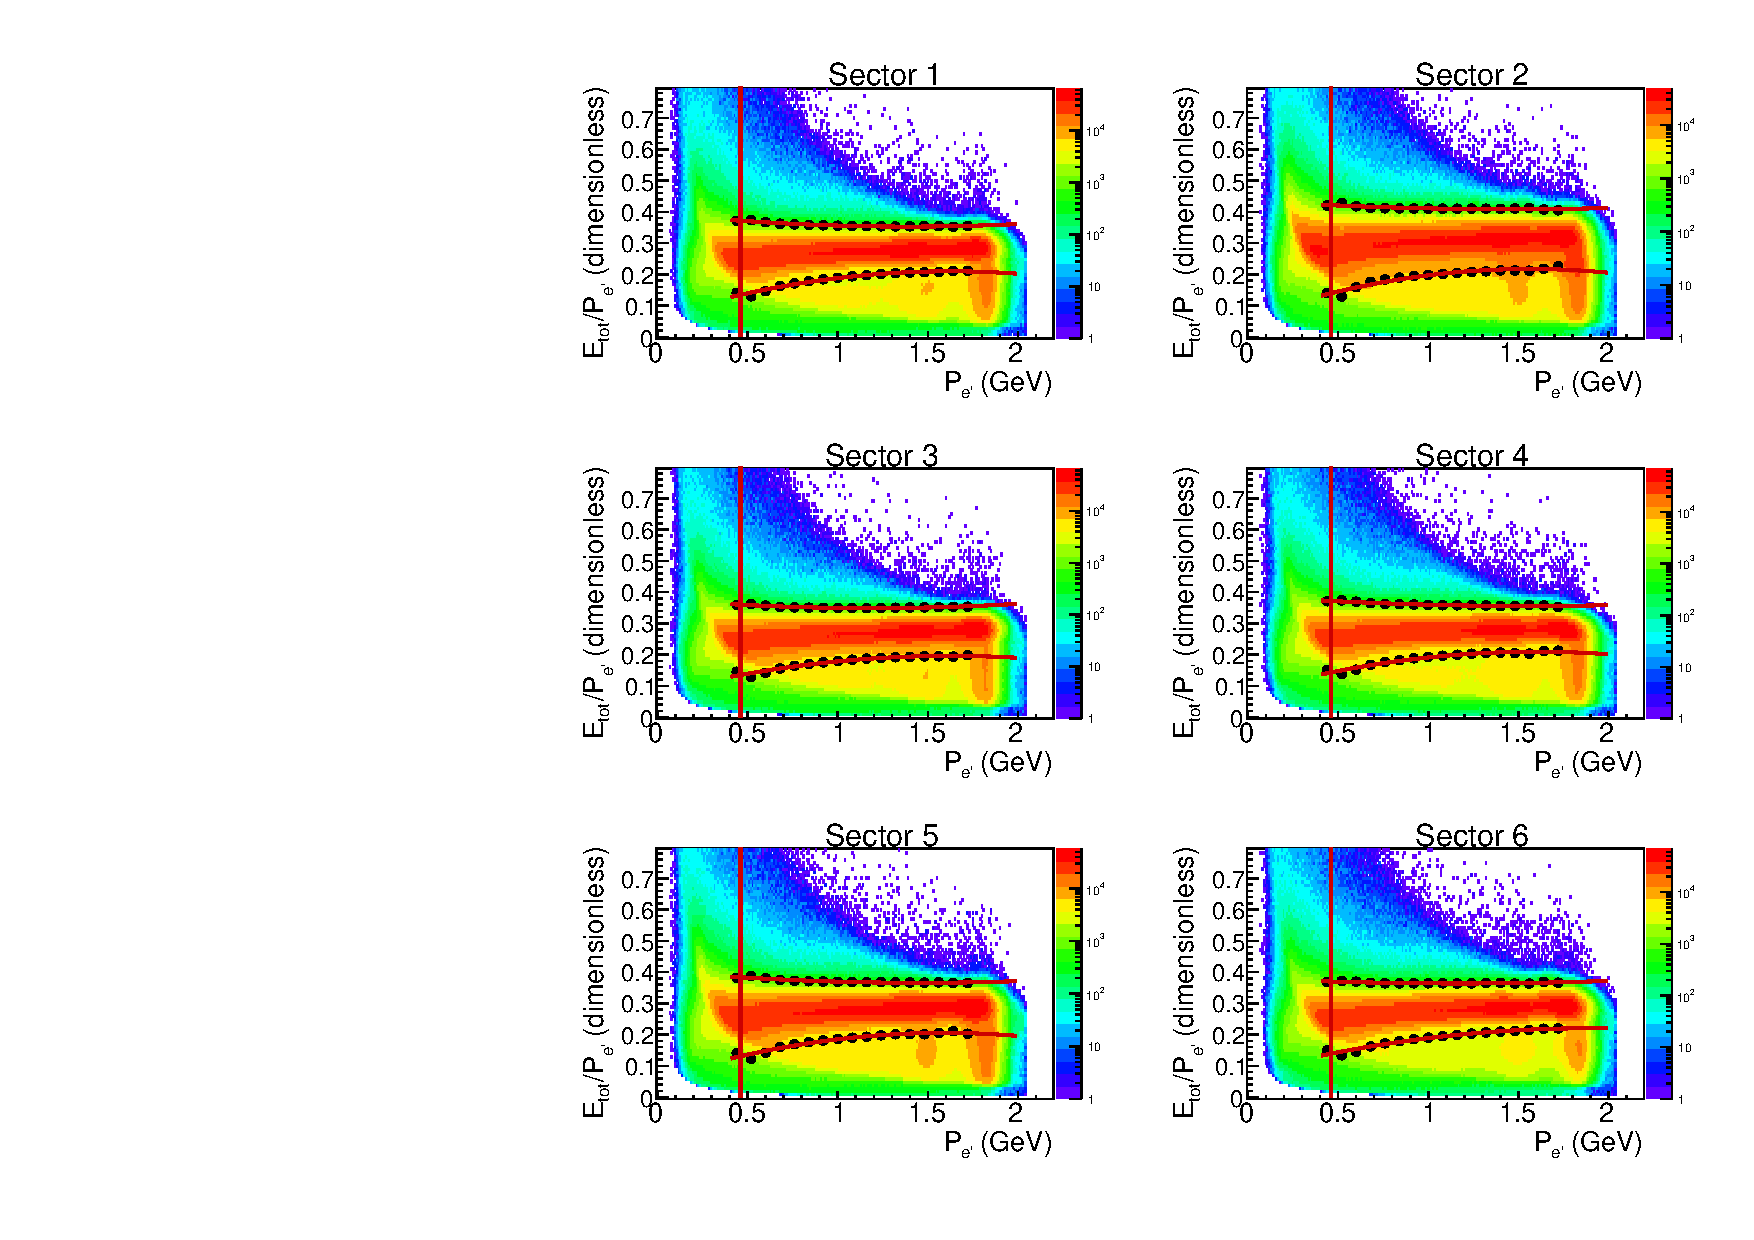
\includegraphics[width=11cm]{pictures/event_selection/ec_cut/ectot_cut_data.pdf}}
\caption{\small Sampling fraction distributions for the data. The six plots correspond to the six CLAS sectors. The vertical red line at $P_{e'} = 0.461$~GeV shows the EC threshold cut. Black points correspond to the positions of Gaussian fit maxima $\pm 3\sigma$ for different $X$-slices of the 2D histograms. These points are fit by a second order polynomial, the resulting functions are shown by the red curves. Events between the red curves are selected for further analysis.} \label{fig:ec_cut_data}
\end{center}
\end{figure}

\begin{figure}[htp]
\begin{center}
\framebox{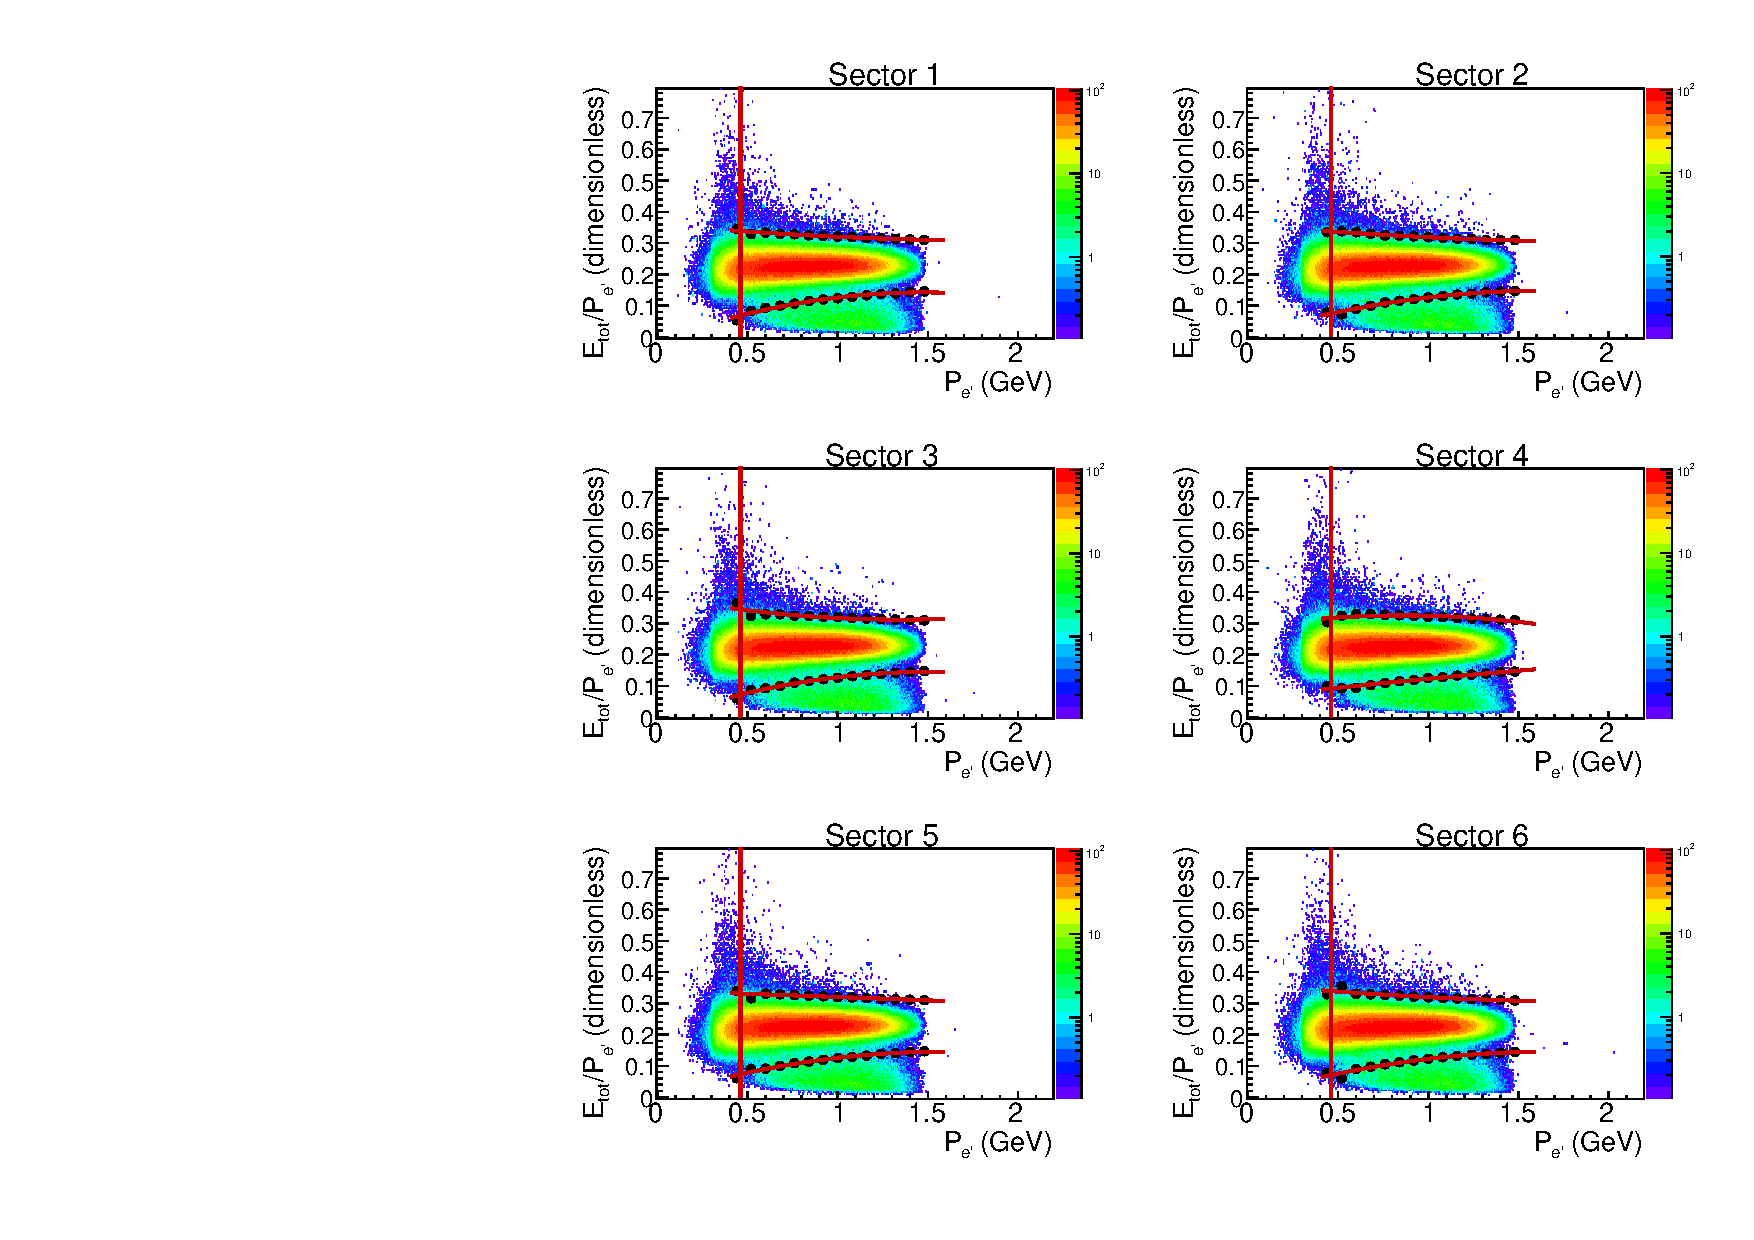
\includegraphics[width=11cm]{pictures/event_selection/ec_cut/ectot_cut_sim.pdf}}
\caption{\small  Sampling fraction distributions for the reconstructed Monte Carlo events. The six plots correspond to the six CLAS sectors. The vertical red line at $P_{e'} = 0.461$~GeV shows the EC threshold cut. Black points correspond to the positions of Gaussian fit maxima $\pm 3\sigma$ for different $X$-slices of the 2D histograms. These points are fit by a second order polynomial, the resulting functions are shown by the red curves. Events between red curves are selected for further analysis.} \label{fig:ec_cut_sim}
\end{center}
\end{figure}



Then, the so-called sampling fraction cut is applied to eliminate part of the pion contamination. To develop this cut, the fact that electrons and pions have different energy deposition patterns in the EC is used. An electron produces an electromagnetic shower, where the deposited energy $E_{tot}$ is proportional to the scattered electron momentum $P_{e'}$, while a $\pi^{-}$ loses a constant amount of energy per scintillator ($\sim 2$~MeV/cm) independently of its momentum. Therefore, for electrons the quantity $E_{tot}/P_{e'}$ plotted as a function of $P_{e'}$ should follow the straight line that is parallel to the $x$-axis and located around the value 1/3 on the $y$-axis, since electrons lose about 2/3 of their energy in lead sheets (in reality this line has a slight slope).


In Fig.~\ref{fig:ec_cut_data} the total energy deposited in the EC divided by the particle momentum is shown as a function of particle momentum. The six plots correspond to the six CLAS sectors. Events between the red curves are selected as good electron candidates for further analysis. The vertical red line at $P_{e'} = 0.461$~GeV shows the EC threshold cut. The upper and lower red curves are obtained in the following way:  $X$-slices of the 2D histograms are fit by Gaussians. In this way points that correspond to the positions of the fit maxima $\pm 3\sigma$ are obtained. These points are shown by black circles in Fig.~\ref{fig:ec_cut_data}. They determine the upper and lower boundaries for the cut. Finally, to obtain smooth curves, all points are fit by a second order polynomial.  



Cuts on the minimal electron momentum and on sampling fraction are applied both to the experimental and reconstructed Monte Carlo events. Since the Monte Carlo simulation does not reproduce electromagnetic showers well enough, the sampling fraction distributions for the simulation are slightly lower than for the data. EC cuts for the simulation, obtained using the same  procedure as for the data, are shown in Fig.~\ref{fig:ec_cut_sim}. These plots contain no events with $P_{e'} > 1.5$~GeV since only double-pion events were generated, while for the data events with $P_{e'} > 1.5$~GeV exist since Figure~\ref{fig:ec_cut_data} was plotted for inclusive electrons.



\subsubsection{CC cuts}
\label{Sect:cc_cuts} 
To improve the quality of the electron candidate selection and $\pi^{-}/e^{-}$ separation, a \v Cerenkov counter is used~\cite{Adams:2001kk}. As shown in~\cite{Osipenko:2004}, there is a contamination in the measured CC spectra that manifests itself as a so-called single-photoelectron peak, which is actually located at a few photoelectrons (see the distributions shown in black in Fig.~\ref{fig:nphe_all_seg}). The main source of this contamination are accidental coincidences of PMT noise signals with measured pion tracks~\cite{Osipenko:2004}. The goal of CC cuts is to separate the spectrum of good electron candidates (it corresponds to the main maximum of the photoelectron distribution) from the single-photoelectron peak, but at the same time to minimize the loss of good events. As seen in Fig.~\ref{fig:nphe_all_seg} (black curves), where photoelectron distributions are plotted, the single-photoelectron peak is rather pronounced and it significantly overlaps with the spectrum of good electron candidates. Thus the elimination of this contamination is not a straightforward task and a special procedure has been developed for this purpose. 

The following set of CC cuts was applied:\vspace{-0.5em}

\begin{itemize}
\item fiducial cut,\vspace{-0.5em}
\item $\varphi_{cc}$ matching cut,\vspace{-0.5em}
\item $\theta_{cc}$ matching cut,\vspace{-0.5em}
\item geometrical cut that removes inefficient zones, and\vspace{-0.5em}
\item standard procedure of dealing with the single-photoelectron peak contamination based on the fit of the photoelectron distributions by the modified Poisson function.
\end{itemize}

All these cuts, except the last one, are defined in the so-called ``CC projective plane"~\cite{Osipenko:2004}. This is an imaginary plane behind the CC where the \v Cerenkov radiation would arrive if its polygonal (due to reflections in the mirror system) path from the emission point to the PMT was substituted by a straight line preserving the initial propagation direction and the total distance traveled~\cite{Osipenko:2004,Adams:2001kk}. The polar and azimuthal angles $(\theta_{cc},\varphi_{cc})$, which are defined in this projective plane, are not directly available in the BOS banks~\cite{BOS:bank}. Therefore, some calculations are made to derive these angles from the variables available in the DCPB bank. Figure~\ref{fig:cc_plane_def} illustrates these calculations.



The CC projective plane is defined in the sector reference coordinate system, i.e. the sector is bisected in the middle by the $xz$-plane with the $z$-axis directed along the beam line. In this reference system the equation of the projective plane is the following (according to Ref.~\cite{Osipenko:2004}),
\begin{equation}
\begin{aligned}
 &Ax+By+Cz+D = 0,  \\ \label{eq:cc_plane}
 &A=-0.000785,~~B=0,  \\
 &C=-0.00168,~~~D=1,  \\
 &\overrightarrow{S} = (A,B,C),
\end{aligned}  
\end{equation}
where $\overrightarrow{S}$ is a vector perpendicular to the projective plane.

In Fig.~\ref{fig:cc_plane_def} the particle track in the DC is shown by the thin dashed curve. Since the particle moves through a magnetic field in the DC, the track is curved. Having left the magnetic field region of the DC, the particle moves further along a straight line, tangential to a curved DC track in the point of its intersection with the CC. The unit vector that defines the direction of this tangent is known from the DCPB bank $ \overrightarrow{n} = (n_{x}, n_{y}, n_{z}) = ($CX\_SC,~CY\_SC,~CZ\_SC$)$. In Fig.~\ref{fig:cc_plane_def} the vector $ \overrightarrow{t}$ is pointing this direction and goes from the SC hit point to the CC projective plane.

\begin{figure}[htp]
\begin{center}
\framebox{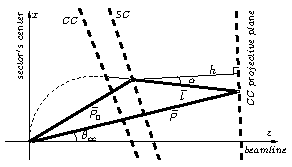
\includegraphics[width=10cm]{pictures/event_selection/cc_cut/cc_plane_def_new.pdf}}
\caption{\small  Illustration for the calculation of the polar $\theta_{cc}$ and azimuthal $\varphi_{cc}$ angles in the CC projective plane (see text for details).} \label{fig:cc_plane_def}
\end{center}
\end{figure}


The $(\theta_{cc},\varphi_{cc})$ angles in the projective plane are determined by the vector $\overrightarrow{P}=\overrightarrow{P_{0}}+\overrightarrow{t}$, where $\overrightarrow{P_{0}}$ is a vector that goes from the vertex to the point of the track intersection with the SC. Its components are known from the DCPB bank\footnote[3]{In the DCPB bank both $\overrightarrow{n}$ and $\overrightarrow{P_{0}}$ are defined in the sector reference frame.} $\overrightarrow{P_{0}} = (p_{x}^{0},p_{y}^{0},p_{z}^{0}) = ($x\_SC,~y\_SC,~z\_SC$)$.

The vector $\overrightarrow{t}$ can be defined as
\begin{equation}
 \overrightarrow{t} =  | \overrightarrow{t}  |\cdot \overrightarrow{n}  =  \frac{h}{\cos \alpha}\cdot \overrightarrow{n},
\label{eq:cc_t_vec} 
\end{equation}
where $\overrightarrow{n}$ is the unit vector in the $\overrightarrow{t}$-direction defined above, while $h$ is the distance from the SC hit point to the CC projective plane, which is given by\footnote[4]{This is a standard relation for the distance from the point (given here by the vector $\overrightarrow{P_{0}}$) to the plane $Ax+By+Cz+D = 0$. }
\begin{equation}
h=\frac{|(\overrightarrow{S} \cdot \overrightarrow{P_{0}})+D|}{ |\overrightarrow{S}  |},
\label{eq:cc_h_distance}
\end{equation}
where $\overrightarrow{S}$ is the vector normal to the CC projective plane defined by Eq.~\eqref{eq:cc_plane}.

In turn $\cos \alpha$ can be calculated as
\begin{equation}
\cos \alpha = \frac{|(\overrightarrow{S}\cdot \overrightarrow{n})|}{|\overrightarrow{S}|},
\end{equation}
since $\overrightarrow{S}$ is directed along $h$ and $\overrightarrow{n}$ is directed along $\overrightarrow{t}$. 



This leads to the following expression for the vector $\overrightarrow{t}$,
\begin{equation}
 \overrightarrow{t} =  | \overrightarrow{t}  |\cdot \overrightarrow{n}  =\left | \frac{(\overrightarrow{S} \cdot \overrightarrow{P_{0}})+D}{(\overrightarrow{S} \cdot \overrightarrow{n})}\right |\cdot \overrightarrow{n}   = \left | \frac{A\! \cdot\! p_{x}^{0}+B\! \cdot\! p_{y}^{0}+C\! \cdot\! p_{z}^{0}+D}{A \!\cdot\! n_{x}+B\! \cdot\! n_{y}+C \!\cdot\! n_{z}}\right |\cdot\overrightarrow{n}.
\label{eq:cc_t_vec} 
\end{equation}


Then, obtaining the required vector $\overrightarrow{P}$ as the sum of $\overrightarrow{P_{0}}$ and $\overrightarrow{t}$, one can finally calculate the angles $\theta_{cc}$ and $\varphi_{cc}$ as 
\begin{equation}
\begin{aligned}
\theta_{cc}&=\arccos\left ( \frac{P_z}{| \overrightarrow{P}  |}\right ),\\
\varphi_{cc} & =  \arctan\left ( \frac{P_{y}}{P_{x}} \right ). 
\label{eq:cc_phi_theta} 
\end{aligned}
\end{equation}

The angle $\varphi_{cc}$ defined by Eq.~\eqref{eq:cc_phi_theta} is determined with respect to the center of each sector. This means that $\varphi_{cc} = 0$ is the middle of the sector, $\varphi_{cc} < 0$ is on the left side of the sector, and $\varphi_{cc} > 0$ is on its right side.

One should also define the variables $CC~segment~number$ (that indicates which segment has been hit) and $index$ (that indicates which PMT has fired). They are taken from the CCPB bank $Status$ variable according to the following relation,
\begin{equation}
Status = 10\times(\text{CC segment number}) + 1000\times( 1 + index),
\label{eq:cc_segment}
\end{equation}
where $index$ is 1 for right PMTs, $-1$ for left PMTs, and 0 when both PMTs have fired.



%---------------------------------------------------------------------------------

After all needed variables have been defined, all the cuts from the list specified above can be implemented.

First of all the fiducial cut in the CC plane is applied. The shape of this cut is taken from~\cite{Khetarpal:2010} and is given by
\begin{equation}
\begin{aligned}
\theta_{cc} > 7.0+0.0032\cdot \varphi_{cc}~+~&0.0499\cdot \varphi_{cc}^{2}, \\
\left( \frac{\theta_{cc}-45.5^{o}}{34.5^{o}} \right)^{2} + \left( \frac{\varphi_{cc}}{21^{o}} \right)^{2} &\le 1, \\
\left( \frac{\theta_{cc}-45.5^{o}}{1.75^{o}} \right)^{2} + \left( \frac{\varphi_{cc}}{21^{o}} \right)^{2} &> 1,~\textrm{and} \\
\theta_{cc} < 45^{o}. \, \, \,  \, \, \, \, \, \,   \, \, \,  \, \, \, \, \, \,
\label{eq:cc_fiduch}
\end{aligned}
\end{equation}\vspace{-1em}

Then the so-called $\varphi_{cc}$ and $\theta_{cc}$ matching procedures (based on the studies~\cite{Osipenko:2004} and~\cite{Ungaro:2010}) are performed. The idea of this matching is quite simple: there must be one-to-one correspondence between the angles in the CC plane (which are calculated based on the information from the DC) and PMT signals in the CC for real events, while background noise and accidentals should not show such correlation.

The principle of the $\varphi_{cc}$ matching cut is the following: when the track is on the right side of the CC segment, the right PMT should be fired, and vice versa. Therefore, if $\varphi_{cc}<0$, the $index$ defined in Eq.~\eqref{eq:cc_segment} is required to be $-1$ and if $\varphi_{cc}>0$, the $index$ is required to~be~1. Events that do not satisfy these conditions are removed. All events with $index=0$ are kept.

\begin{figure}[htp]
\begin{center}
\framebox{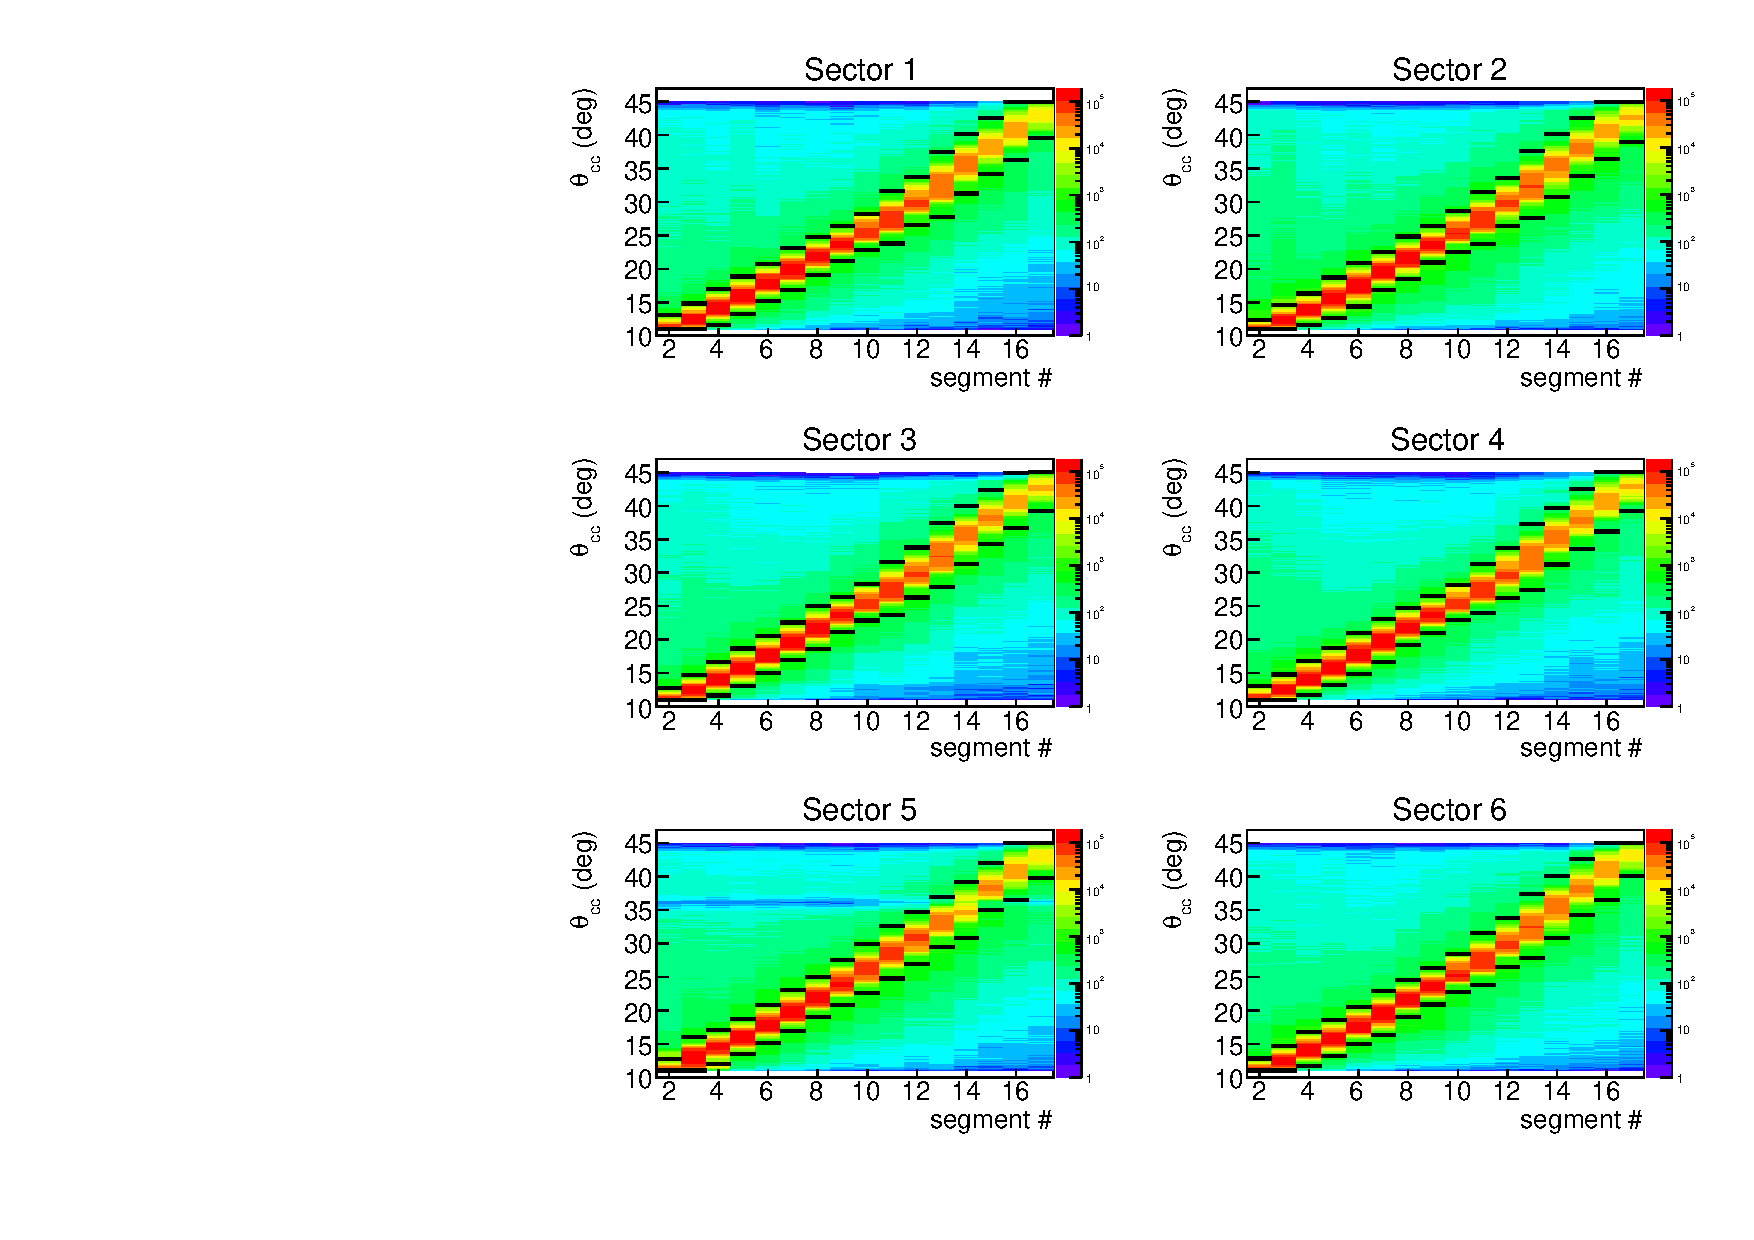
\includegraphics[width=9cm]{pictures/event_selection/cc_cut/th_vs_seg.pdf}}
\caption{\small  $\theta_{cc}$ versus segment distributions for six CLAS sectors. Events between the horizontal black lines are treated as good electron candidates.} \label{fig:th_vs_seg}
\end{center}
\end{figure}%\vspace{-1em}


In order to perform $\theta_{cc}$ matching, the $\theta_{cc}$ versus segment number cut should be done. Figure~\ref{fig:th_vs_seg} shows $\theta_{cc}$ versus segment distributions for the six CLAS sectors. Event distributions in each segment have been plotted as a function of $\theta_{cc}$ and fit by Gaussians. The horizontal black lines correspond to the positions of the fit maxima $\pm4\sigma$. Events between these black lines are treated as good electron candidates.


The influence of $\varphi_{cc}$ and $\theta_{cc}$ matching cuts on the photoelectron distributions is demonstrated in Fig.~\ref{fig:nphe_all_seg}, where the distributions before matching cuts are plotted in black, distributions after the $\varphi_{cc}$ matching are plotted in red, and after the subsequent $\theta_{cc}$ versus segment cut are plotted in blue. As seen in Fig.~\ref{fig:nphe_all_seg} both these cuts reduce the single-photoelectron peak, but leave the main part of the spectrum unchanged. The same $\varphi_{cc}$ and $\theta_{cc}$ matching cuts are also applied to the reconstructed Monte Carlo events.


The accidental noise and pion background are not the only source of the single-photoelectron peak contamination. The peak also partially corresponds to electrons that hit some specific geometrical zones with low CC efficiency. When an electron hits such a zone the number of detected photoelectrons turns out to be significantly less than expected. This leads to the fact that the region of the photoelectron spectrum, which corresponds to the low number of photoelectrons, appears to be overpopulated by events. Since low efficiency zones are distributed inhomogeneously in the CC plane and the Monte Carlo simulation do not reproduce them properly, it is better to remove them from the consideration completely. For this purpose  a special geometrical cut is established. 


This geometrical cut is done in the following way. Distributions $\varphi_{cc}$ versus $\theta_{cc}$ are plotted for each CLAS sector (see Fig.~\ref{fig:ph_vs_th_cc}, upper frame) with the quantity~\eqref{eq:cc_ratio} as a color code. 
\begin{equation}
\frac{number\,\, of\,\, events\,\,  inside\,\, (\theta_{cc},\varphi_{cc})\,\, bin\,\, with\,\, more\,\, than\,\, five\,\, photoelectrons }{total\,\, number\,\, of\,\, events\,\,  inside\,\, (\theta_{cc},\varphi_{cc})\,\, bin}
\label{eq:cc_ratio}
\end{equation}%\vspace{-1em}

This quantity varies from zero to one and shows the proportion of electron candidates with number of photoelectrons greater than five inside a $(\theta_{cc},\varphi_{cc})$ bin. The value for this criterion (five photoelectrons) was chosen rather arbitrarily, since its only purpose is to facilitate the separation of inefficient zones (which correspond mostly to low numbers of photoelectrons) from the regular zones (which correspond to the full photoelectron spectrum). 

The curved vertical stripe in sector five in Fig.~\ref{fig:ph_vs_th_cc} corresponds to an inefficient zone that will be discussed further in~Sec.~\ref{Sect:fiduc_neg}.

\begin{figure}[htp]
\begin{center}
\framebox{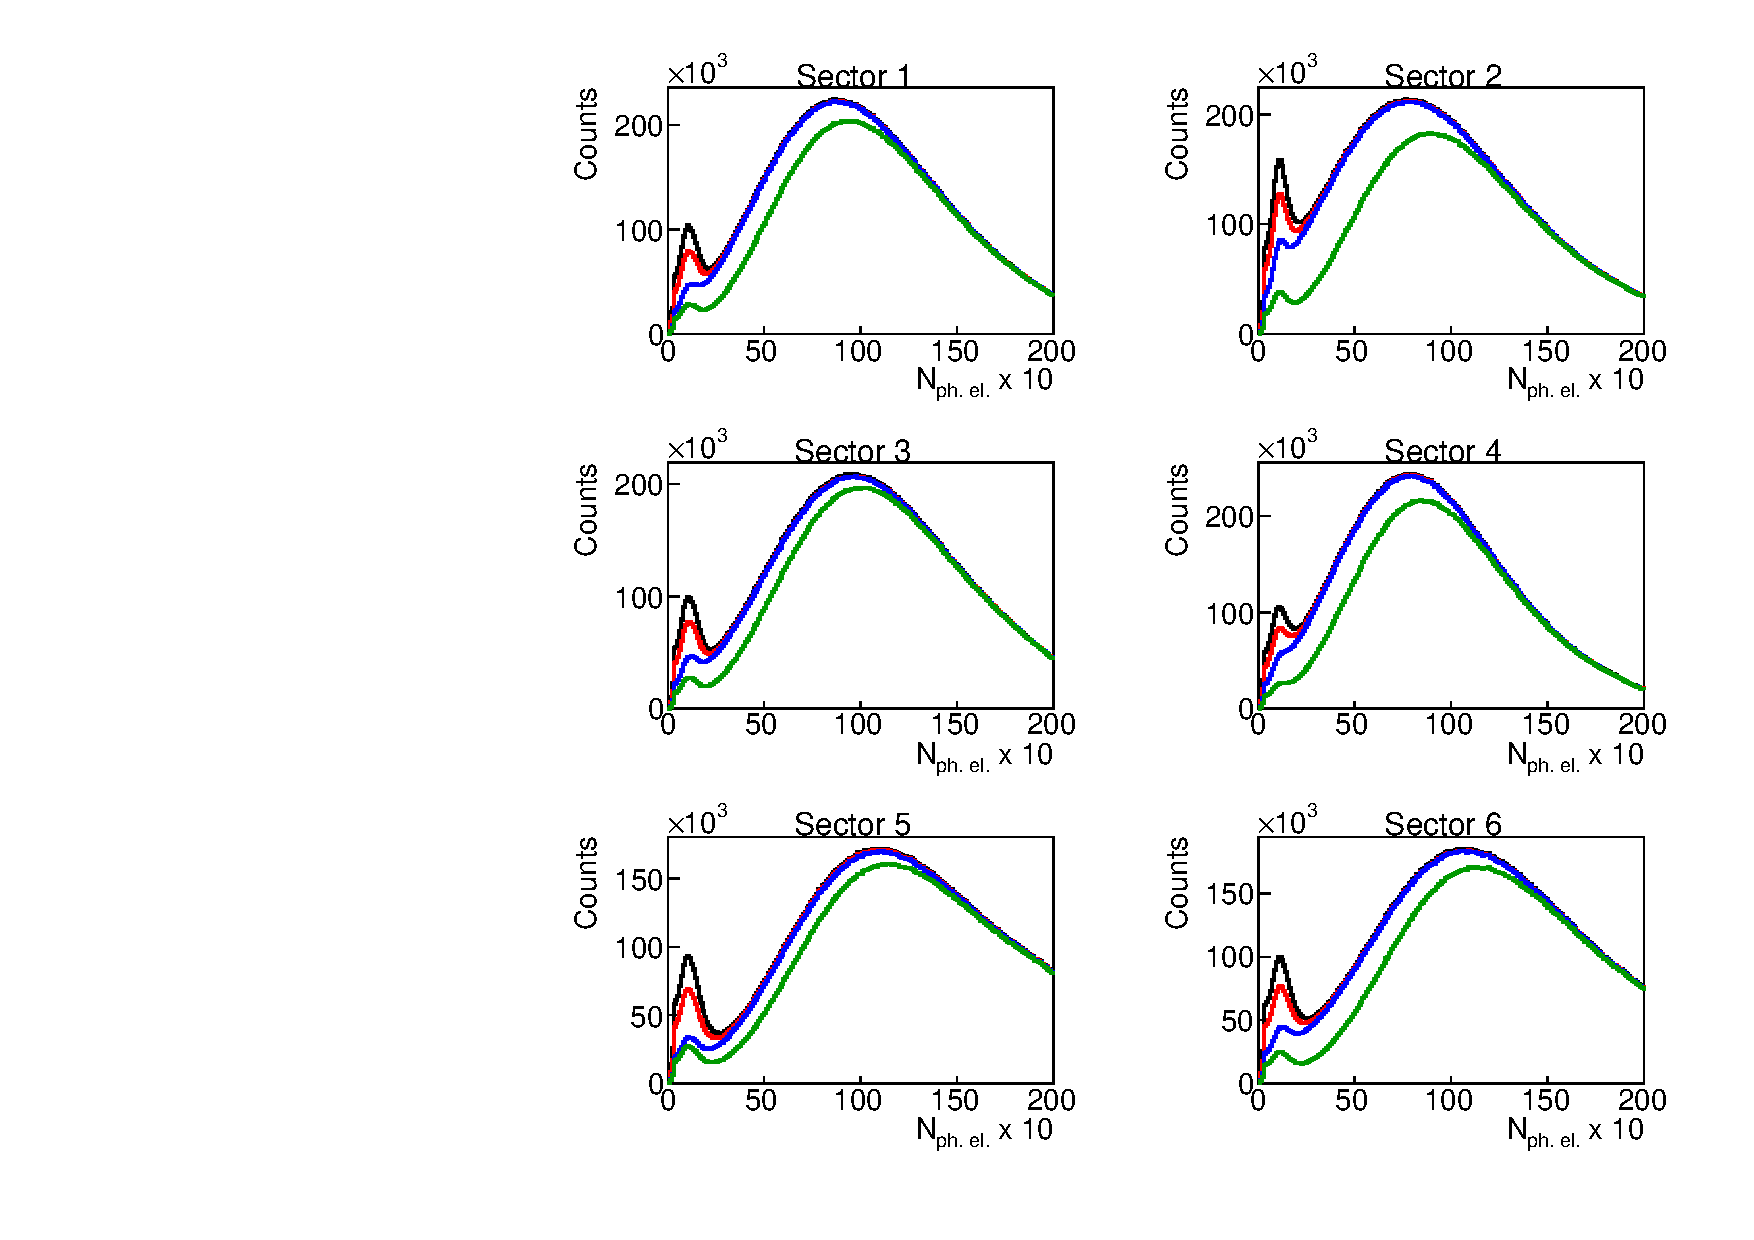
\includegraphics[width=9cm]{pictures/event_selection/cc_cut/nphe_all_seg_bef_aft_diff_cuts.pdf}}
\caption{\small Influence of different CC cuts on the distributions of the number of photoelectrons multiplied by ten for the six CLAS sectors. Black curve -- only fiducial cut in the CC plane is applied, red curve -- the $\varphi_{cc}$ matching cut is added, blue curve -- the $\theta_{cc}$ matching cut is added, and green curve -- the geometrical cut in the CC plane that removes inefficient zones is finally added.} \label{fig:nphe_all_seg}
\end{center}
\end{figure}


For further analysis only fiducial areas with a ratio~\eqref{eq:cc_ratio} greater than the certain threshold value are selected. This threshold value was chosen to be 0.7, 0.65, 0.7, 0.65, 0.8, and 0.8 for sectors 1, 2, 3, 4, 5, and 6, respectively. Since inefficient zones are not identical for various CLAS sectors (see Fig.~\ref{fig:ph_vs_th_cc}), different threshold values are needed for them. Geometrical zones, which are selected for further analysis, are shown in black in the lower plots of Fig.~\ref{fig:ph_vs_th_cc}. All zones shown in white are treated as inefficient and are removed from the analysis. As seen in Fig.~\ref{fig:ph_vs_th_cc}, there is an inefficient zone in the middle of each sector. This is expected since two CC mirrors are joined here. 

\begin{figure}[htp]
\begin{center}
\framebox{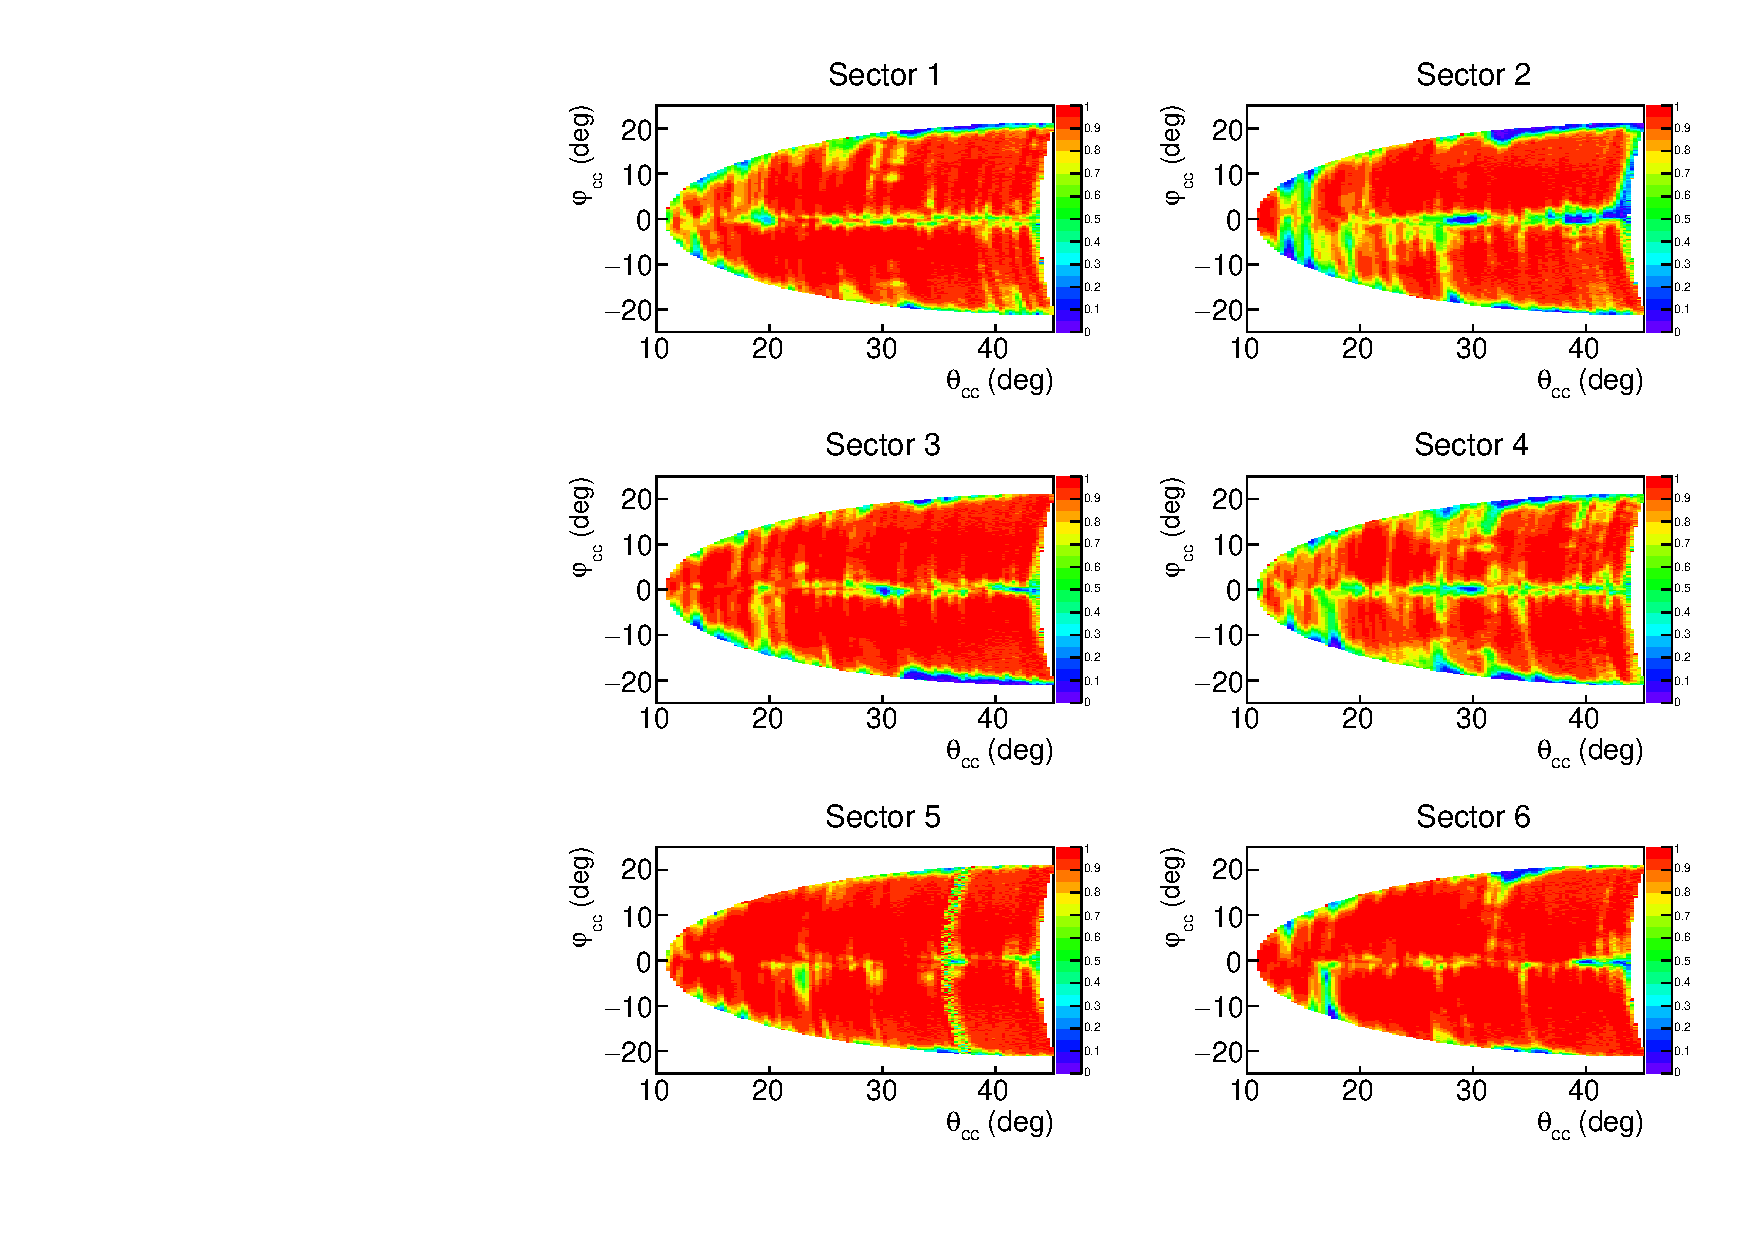
\includegraphics[width=9cm]{pictures/event_selection/cc_cut/cc_2dim_hists_div.pdf}}
\framebox{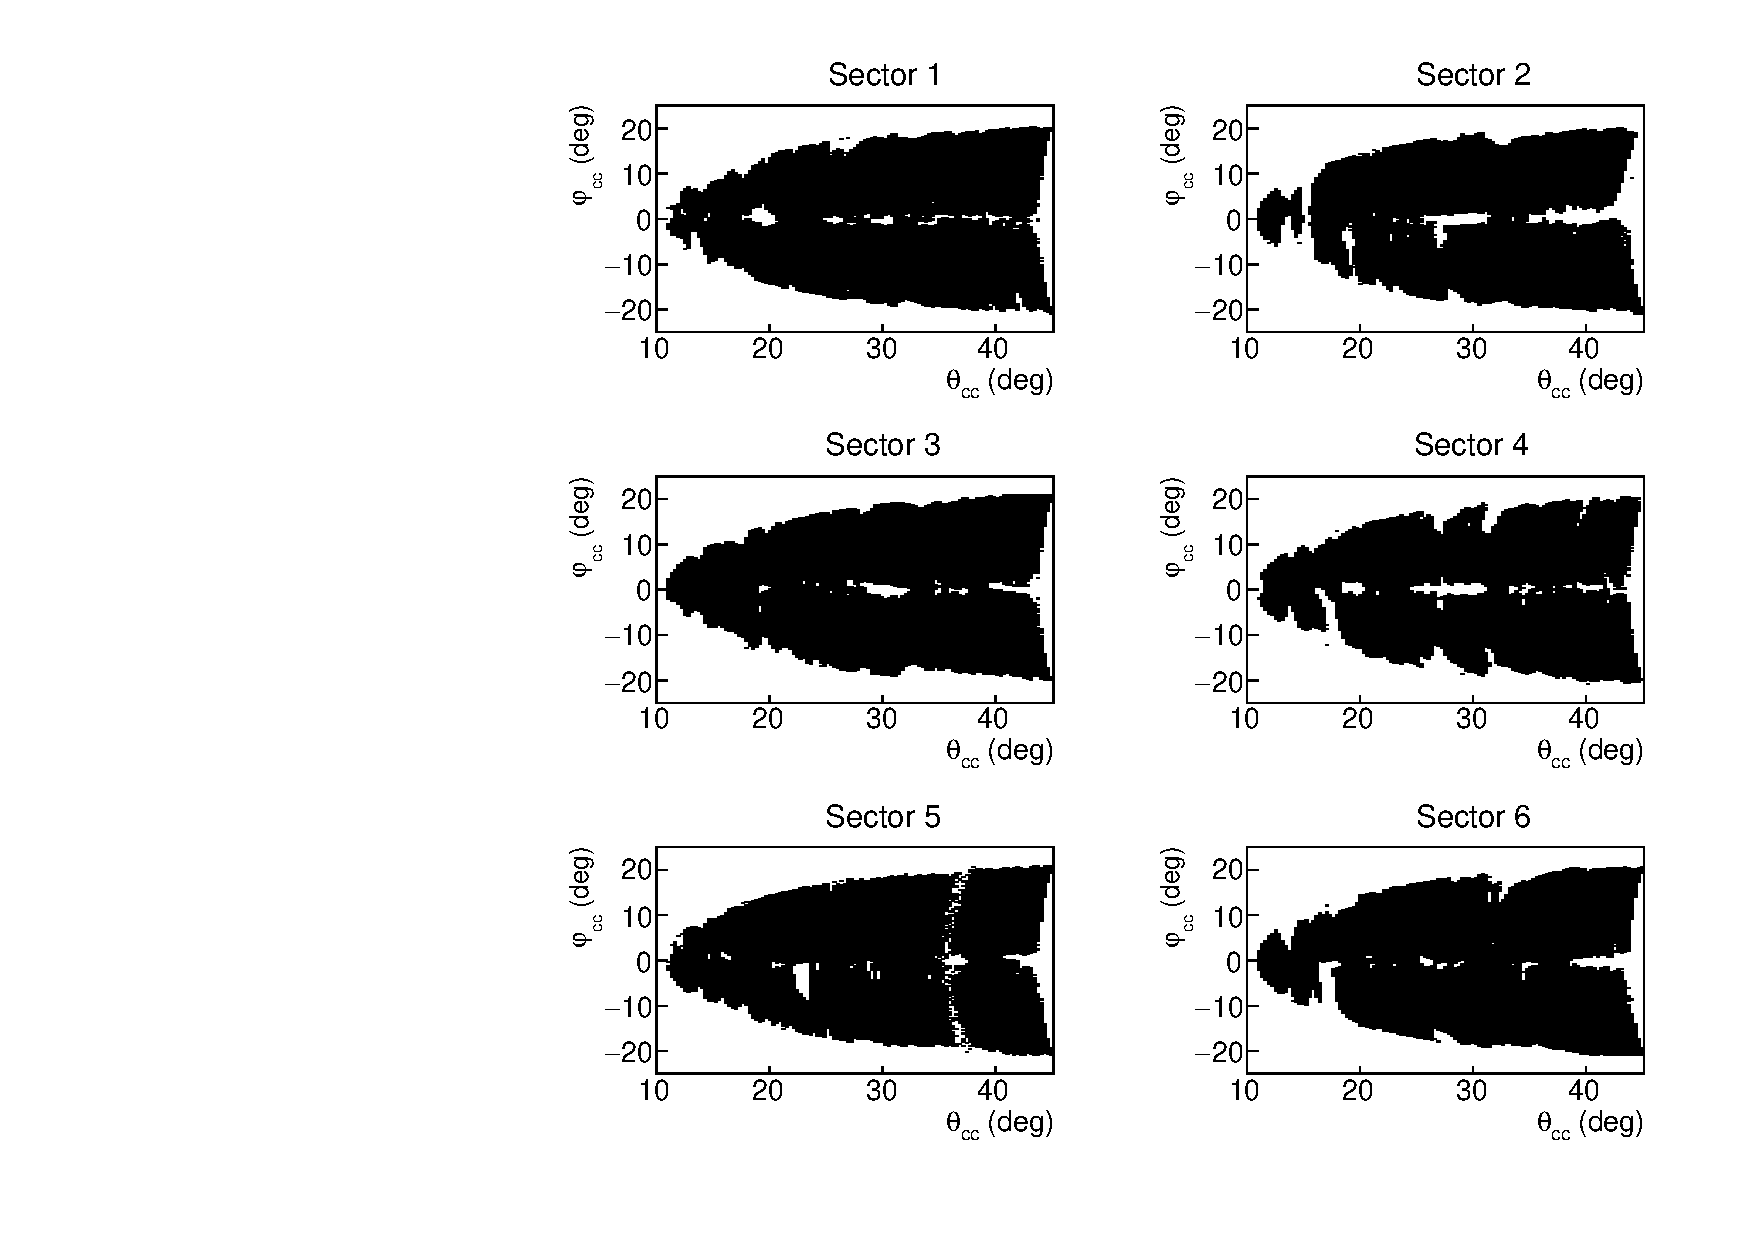
\includegraphics[width=9cm]{pictures/event_selection/cc_cut/cc_geom_cut_gt_065_07_08.pdf}}
\caption{\small Upper frame: Distributions of the quantity~\eqref{eq:cc_ratio} as a function of the polar $\theta_{cc}$ and azimuthal $\varphi_{cc}$ angles in the CC plane for the six CLAS sectors. This quantity varies from zero to one and shows the proportion of electron candidates with number of photoelectrons greater than five inside a $(\theta_{cc},\varphi_{cc})$ bin. Lower frame: Black zones correspond to the fiducial areas with the ratio~\eqref{eq:cc_ratio} greater than 0.7, 0.65, 0.7, 0.65, 0.8, and 0.8 for sectors 1, 2, 3, 4, 5, and 6, respectively. These zones are selected for further analysis. All zones shown in white are treated as inefficient and removed from the analysis.} \label{fig:ph_vs_th_cc}
\end{center}
\end{figure}

The threshold values for the ratio~\eqref{eq:cc_ratio} were chosen in order to keep the balance between the intention to reduce the amount of low efficient zones as much as possible and the desire to preserve most of the statistics. The influence of this geometrical cut on the photoelectron distributions in different sectors is demonstrated in Fig.~\ref{fig:nphe_all_seg}, where the distributions after the cut are plotted in green. As was expected, this cut leads to some reduction in the low lying part of the photoelectron spectrum, including the region of the single-photoelectron peak, and leaves the high lying part of the spectrum unchanged.


This geometrical cut is fully based on the experimental data. It acts as a fiducial cut, because it simply removes certain geometrical regions in the CC plane. This means that it can be safely applied to the Monte Carlo simulation, too. Thus, the same geometrical regions (shown in white in the lower plots in Fig.~\ref{fig:ph_vs_th_cc}) are removed both for the experimental and reconstructed Monte Carlo events.


After the geometrical cut discussed above is applied, the single-photoelectron peak appears to be significantly smaller and better separated from the main spectrum, but still remains (see Fig.~\ref{fig:nphe_all_seg}). Therefore, in order to completely get rid of this contamination, the standard procedure should then be applied~\cite{Fed_an_note:2007}. 


To apply the standard procedure of dealing with the single-photoelectron peak contamination, the photoelectron distributions are plotted for each PMT on the left and right sides of each CC segment and for each CLAS sector (see Fig.~\ref{fig:nphe_cut}). 


In Fig.~\ref{fig:nphe_cut} the red lines show the cuts that are made in order to eliminate events under the single-photoelectron peak. The cut position is individually optimized for each PMT in each sector. The distributions of events, for which both right and left PMTs have fired ($index = 0$) are not subject to this cut, since their contamination caused by the single-photoelectron peak is assumed negligible.


Since the Monte Carlo does not reproduce photoelectron distributions well enough, the cut shown by the red lines in Fig.~\ref{fig:nphe_cut} is applied only to the data. To recover the good electrons that were cut off in this way, a special procedure is applied. The part of the distributions on the right side of the red line is fit by the function~\eqref{eq:cc_Poisson}, which is a slightly modified Poisson distribution. 
\begin{equation}
y = P_{1}\left(\frac{P_{3}^{\frac{x}{P_{2}}}}{\Gamma\left(\frac{x}{P_{2}}+1\right)}
\right)e^{-P_{3}},
\label{eq:cc_Poisson}
\end{equation}
where $P_{1}$, $P_{2}$, and $P_{3}$ are free fit parameters.



The fitting function is then continued into the region on the left side of the red line. In this way the two regions, shown in blue and green in Fig.~\ref{fig:nphe_cut}, are determined. Finally the correction factors are defined by~\eqref{eq:cc_corr_fact} and applied as a weight for each event, which goes to the particular PMT. These correction factors depend on the PMT number and are typically on a level of a few percent.
\begin{equation}
F_{ph.\,\, el.} = \frac{\textrm{\color{green}{green\,\,  area} \color{black}{\,\,+\,\,} \color{blue}{blue\,\,  area}}}{\textrm{\color{green}{green\,\,  area}}}
\label{eq:cc_corr_fact}
\end{equation}

\begin{figure}[htp]
\begin{center}
\framebox{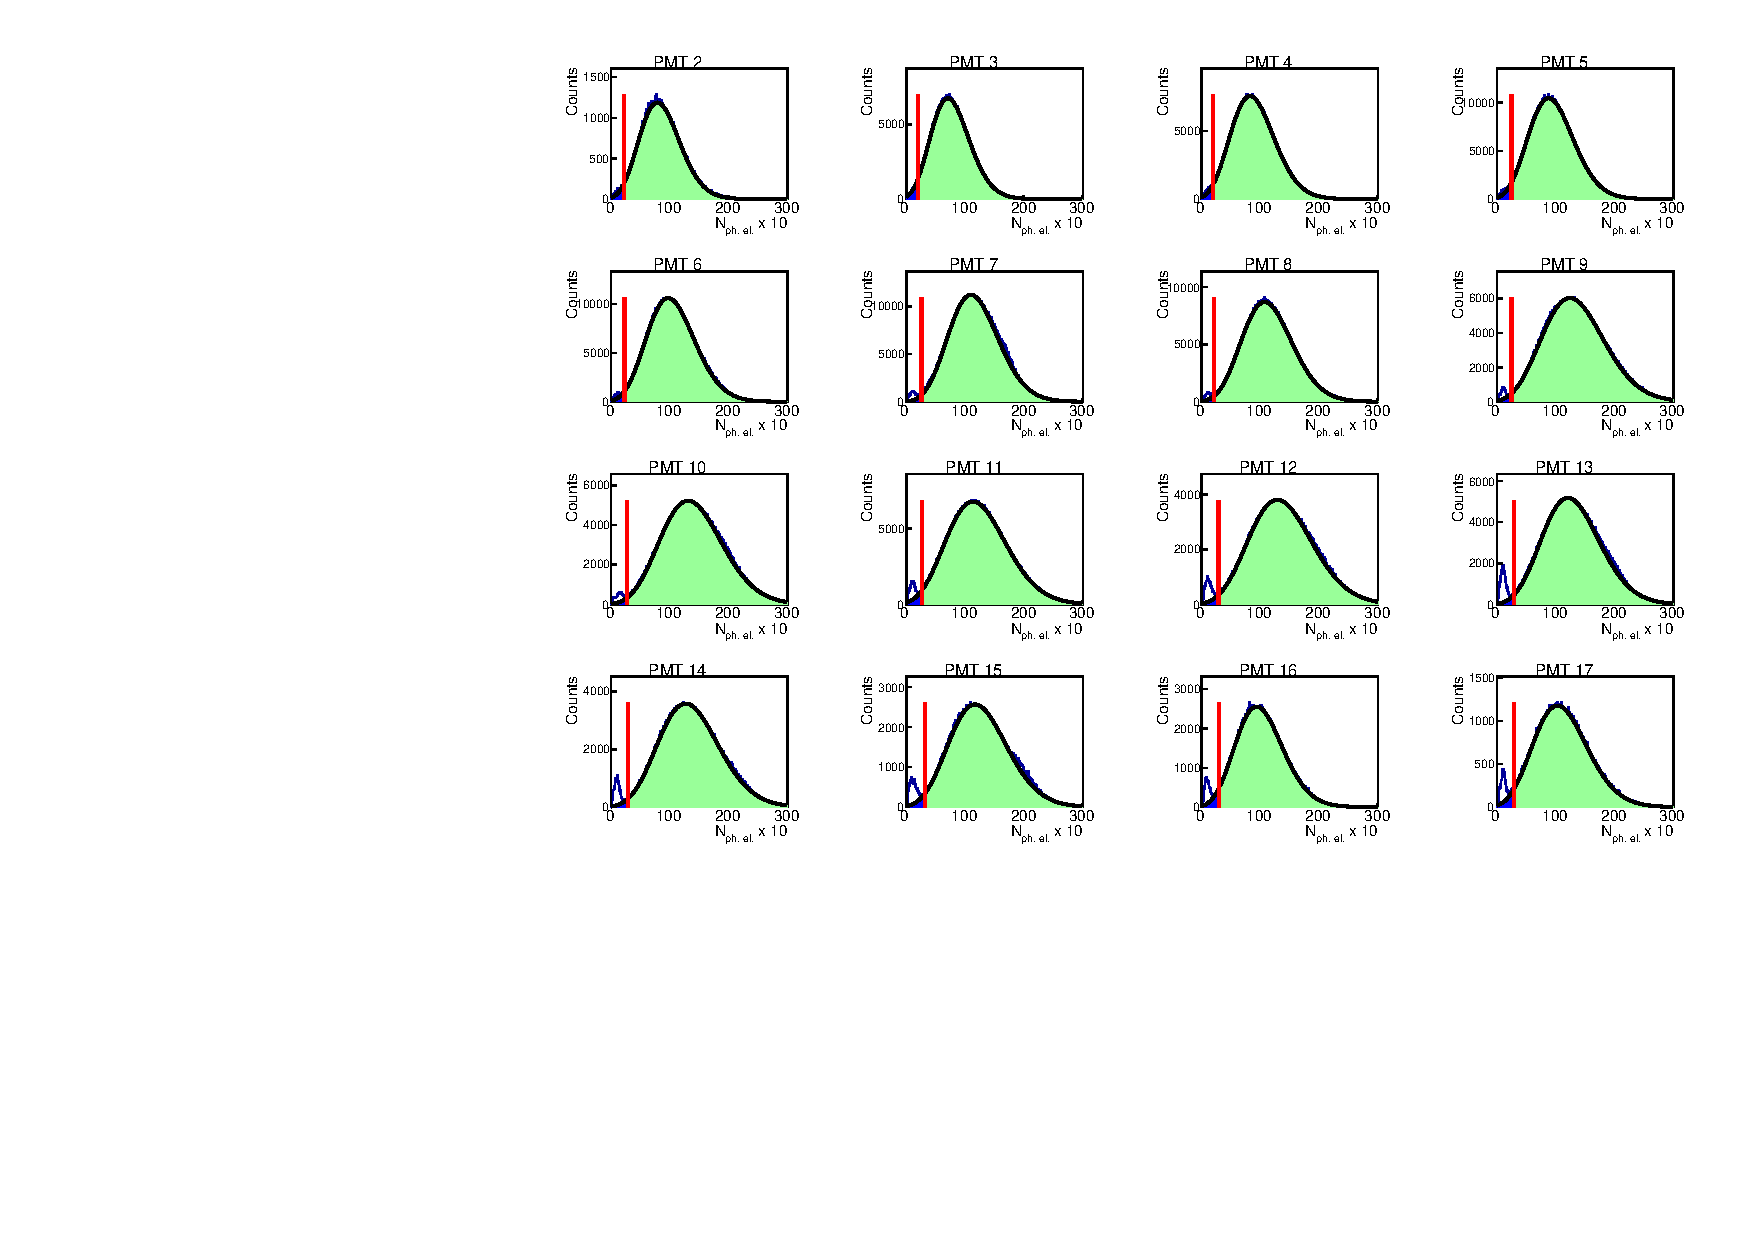
\includegraphics[width=15cm]{pictures/event_selection/cc_cut/ph_el_cut_s1_left_new.pdf}}
\caption{\small Distributions of number of photoelectrons multiplied by ten for the left side of sector one of the CC. Various plots correspond to various CC segments. Black curves show the fit by the function~\eqref{eq:cc_Poisson}. Red vertical lines show the applied cut. Regions that are needed to calculate the correction ratio~\eqref{eq:cc_corr_fact} are shown in blue and green. } \label{fig:nphe_cut}
\end{center}
\end{figure}


Note that segments \#1 and \#18 are removed from the analysis completely (both in data and Monte Carlo), since they are dominated by events from the single-photoelectron peak. 


%-------------------------------------------


\subsection{Hadron identification}
\label{Sect:hadr_id}

% ($\beta_{h} =\frac{v_{h}}{c}$). In this analysis the value of $\beta_{h}$ was derived as the following:
The CLAS TOF system provides information, based on which the particle velocity can be determined. In this analysis for this purpose the following calculations were done.
\begin{equation}
\beta_{h} =\frac{v_{h}}{c}=\frac{l_{h}}{t_{h}\cdot c},
\label{eq:beta_new}
\end{equation}
where $v_{h}$ is the hadron velocity, $c$ the speed of light, $l_{h}$ the hadron path length from the vertex to the SC-plane (variable \textit{Path} in the SCPB bank), and $t_{h}$ the time that it took the hadron to travel from the vertex to the SC-plane. This time can be calculated in the following way. 
\begin{equation}
t_{h} = t_{e} + (t^{tof}_{h}- t^{tof}_{e}) = \frac{l_{e}}{c} + (t^{tof}_{h}- t^{tof}_{e})  ,
\label{eq:time_hadron}
\end{equation}
where $t_{e} = \frac{l_{e}}{c}$ is the time that the electron spent on traveling from the vertex to the SC-plane and $l_{e}$ the electron path length. $t^{tof}_{e}$ and $t^{tof}_{h}$ are the times, when the electron and hadron hit the SC-plane, respectively (the variable \textit{Time} in the SCPB bank).

Equation~\eqref{eq:time_hadron} assumes that the hadron and electron departed from the vertex at the same time, but the electron traveling with the speed of light reached the SC-plane earlier than the hadron. The difference $t^{tof}_{h} - t^{tof}_{e}$ indicates the hadron delay time, which is the consequence of traveling with the velocity $v_{h}<c$. Thus Eq.~\eqref{eq:time_hadron} makes the hadron time related to that of electron for each event\footnote[5]{It worth noting that usually one uses the value of $\beta$ directly defined in the EVNT bank (variable \textit{Betta}), but it turned out that this quantity shows noticeable inaccuracies in electron bunch determination, which were made during the cooking. The value of $\beta$ calculated by Eqs.~\eqref{eq:beta_new} and ~\eqref{eq:time_hadron} do not show these inaccuracies because in this method the timing of the hadron is related to that of electron for each event. }.  

The charged hadron can be identified by the comparison of $\beta_{h}$ determined from TOF according to Eqs.~\eqref{eq:beta_new} and ~\eqref{eq:time_hadron} with $\beta_{n}$ given by 
\begin{equation}
\beta_{n}=\frac{p_{h}}{\sqrt{p_{h}^{2}+m_{h}^{2}}}.
\label{eq:hadron_hadronmass}
\end{equation}

In Eq.~\eqref{eq:hadron_hadronmass} $\beta_{n}$ is a so-called nominal value that is calculated using the particle momentum ($p_{h}$) known from the DC and the exact particle mass assumption ($m_{h}$).

The usual way to develop hadron id cuts is to investigate $\beta$ versus momentum distributions for different TOF paddles for each hadron type separately. This investigation reveals three types of problematic paddles, i.e.

\begin{enumerate}[label=\Alph*]\vspace{-0.5em}
\item  Paddles which signals are completely unreliable (bad paddles). These are paddles \#16 in sector 2, \#44 in sector 3, \#17 in sector 5, and \#48 in each sector. They are excluded from this analysis both for experimental data and reconstructed Monte Carlo events. 
\item Paddles in which the distributions are shifted from their expected positions. The reason for this is most likely mistakes during data cooking/calibration. Typical examples of such paddles are shown in Fig.~\ref{fig:shifted_paddles}.
\item Paddles for which the distributions for a given hadron have double band structure. This problem appears for most of the paddles with number $\geq 40$ and originates from the fact that (along with the mistakes during cooking/calibration) for these paddles two scintillation bars were connected to one TDC~\cite{clas_tof_paddles}. Typical examples of such paddles are shown in Fig.~\ref{fig:double_paddles}.
\end{enumerate}

\begin{figure}[htp]
\begin{center}
\framebox{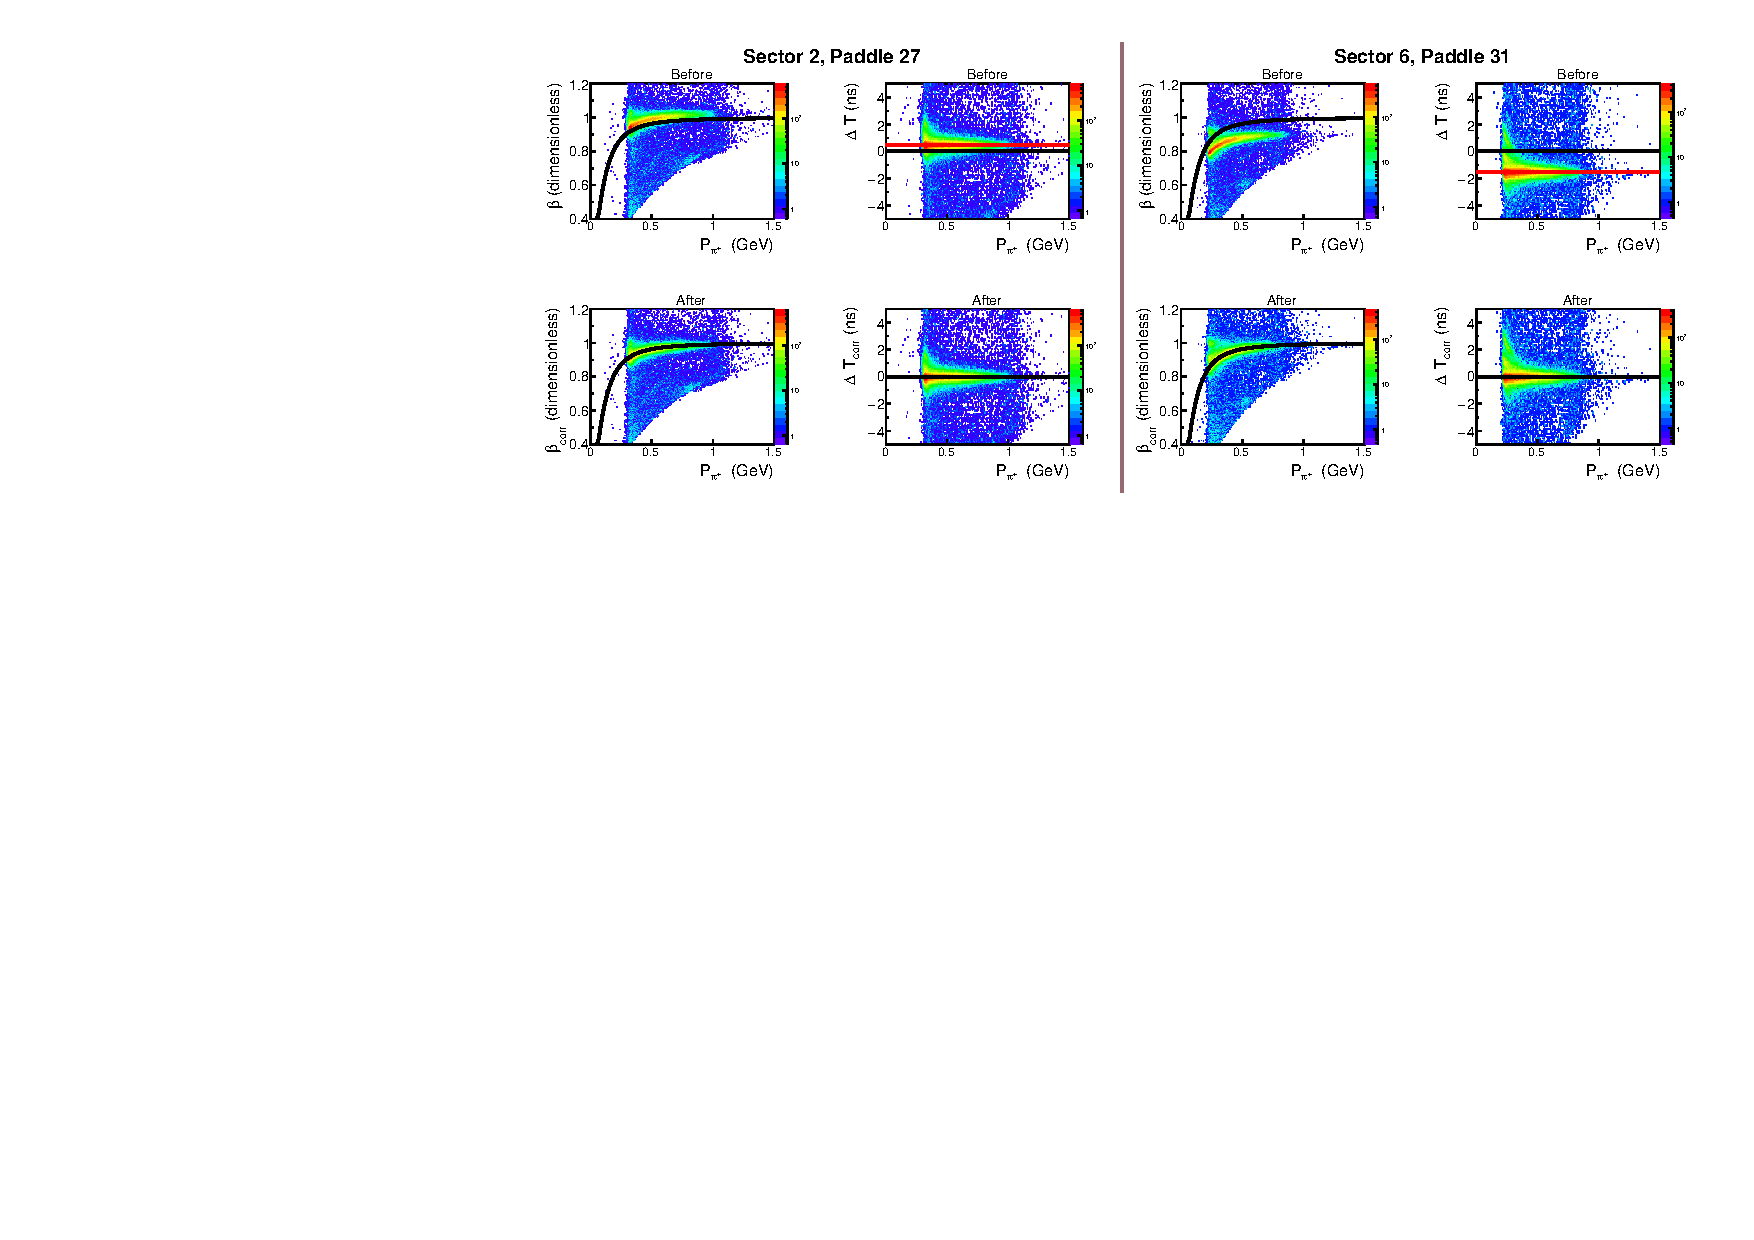
\includegraphics[width=16.3cm]{pictures/event_selection/hadron_id/shifted_paddles.pdf}}
\caption{\small Timing correction for type B problematic paddles \#27 in sector 2 (left side) and \#31 in sector 6 (right side) for $\pi^+$ candidates. The first column in each side shows the $\beta_{h}$ versus momentum distributions with the black curve corresponding to the nominal $\beta_{n}$ defined by Eq.~\eqref{eq:hadron_hadronmass}. The second column in each side corresponds to the $\Delta T$ versus momentum distributions, where the black horizontal line shows the position of zero and the red line shows the position of shifted $\Delta T$-band. The uncorrected distributions are given in the first row, while the influence of the correction is shown in the second row.  \label{fig:shifted_paddles}} 
\end{center}
\end{figure}


To cure the latter two types of problems, a so-called timing correction is developed. To perform this correction, the quantity $\Delta T$ is calculated, which corresponds to the time difference between the real TOF signal and the expected one.
\begin{equation}
\Delta T = \frac{l_{h}}{c}\left (\frac{1}{\beta_{n}} - \frac{1}{\beta_{h}}  \right ).
\label{eq:delta_t}
\end{equation}


Figure~\ref{fig:shifted_paddles} illustrates the timing correction for type B problematic paddles \#27 in sector 2 (left side) and \#31 in sector 6 (right side) for $\pi^+$ candidates. The plots in the first row correspond to the $\beta_{h}$ versus momentum and $\Delta T$ versus momentum distributions before the correction. It is seen that $\beta_{h}$ versus momentum bands are shifted from their expected position shown by the black curve, which corresponds to the nominal $\beta_{n}$ defined by Eq.~\eqref{eq:hadron_hadronmass}. These shifts of $\beta_{h}$ versus momentum bands are caused by the corresponding shifts of the $\Delta T$ versus momentum bands from zero position shown by the black horizontal lines. The idea of the timing correction is to move $\Delta T$ bands back to the position around zero, as shown in the corrected $\Delta T$ versus momentum plots in the second row. The corrected value of $\beta$ is then calculated as
\begin{equation}
\beta_{corr} = \frac{1}{\frac{1}{\beta_{n}} - \frac{(\Delta T-t_{shift})\cdot c}{l_{h}}},
\label{eq:beta_corr}
\end{equation}
where $t_{shift}$ is the position of shifted $\Delta T$-band shown by the corresponding red horizontal line in Fig.~\ref{fig:shifted_paddles}.

The $\beta_{corr}$ versus momentum distributions are shown in second row in Fig.~\ref{fig:shifted_paddles}. As seen in these plots, $\beta_{corr}$ versus momentum bands demonstrate no shift from the black curves after the timing correction is applied.


\begin{figure}[htp]
\begin{center}
\framebox{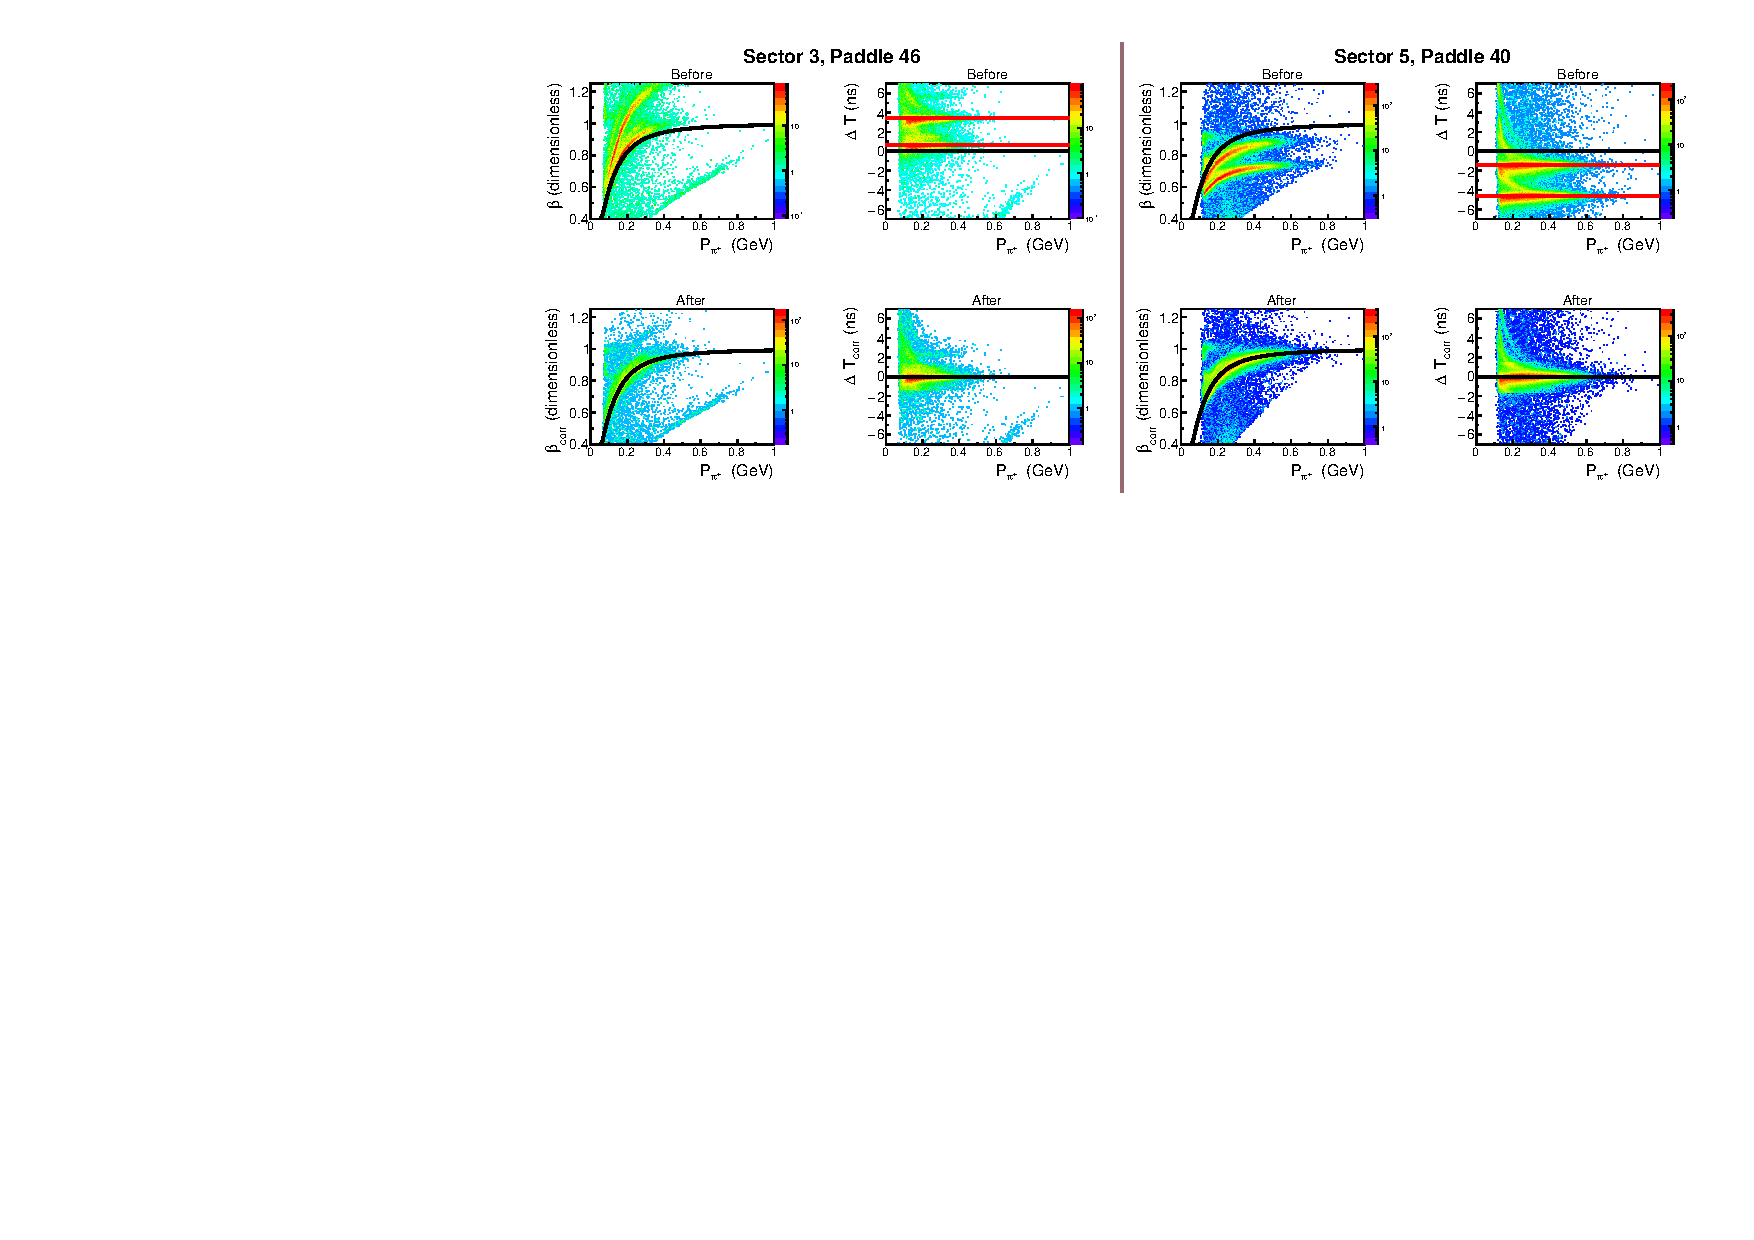
\includegraphics[width=16.3cm]{pictures/event_selection/hadron_id/double_paddles.pdf}}
\caption{\small Timing correction for type C problematic paddles \#46 in sector 3 (left side) and \#40 in sector 5 (right side) for $\pi^+$ candidates. The first column in each side shows the $\beta_{h}$ versus momentum distributions with the black curve corresponding to the nominal $\beta_{n}$ defined by Eq.~\eqref{eq:hadron_hadronmass}. The second column in each side corresponds to the $\Delta T$ versus momentum distributions, where the black horizontal line shows the position of zero and the red lines show the position of shifted $\Delta T$-bands. The uncorrected distributions are given in the first row, while the influence of the correction is shown in the second row. \label{fig:double_paddles}} 
\end{center}
\end{figure}

\begin{figure}[htp]
\begin{center}
\framebox{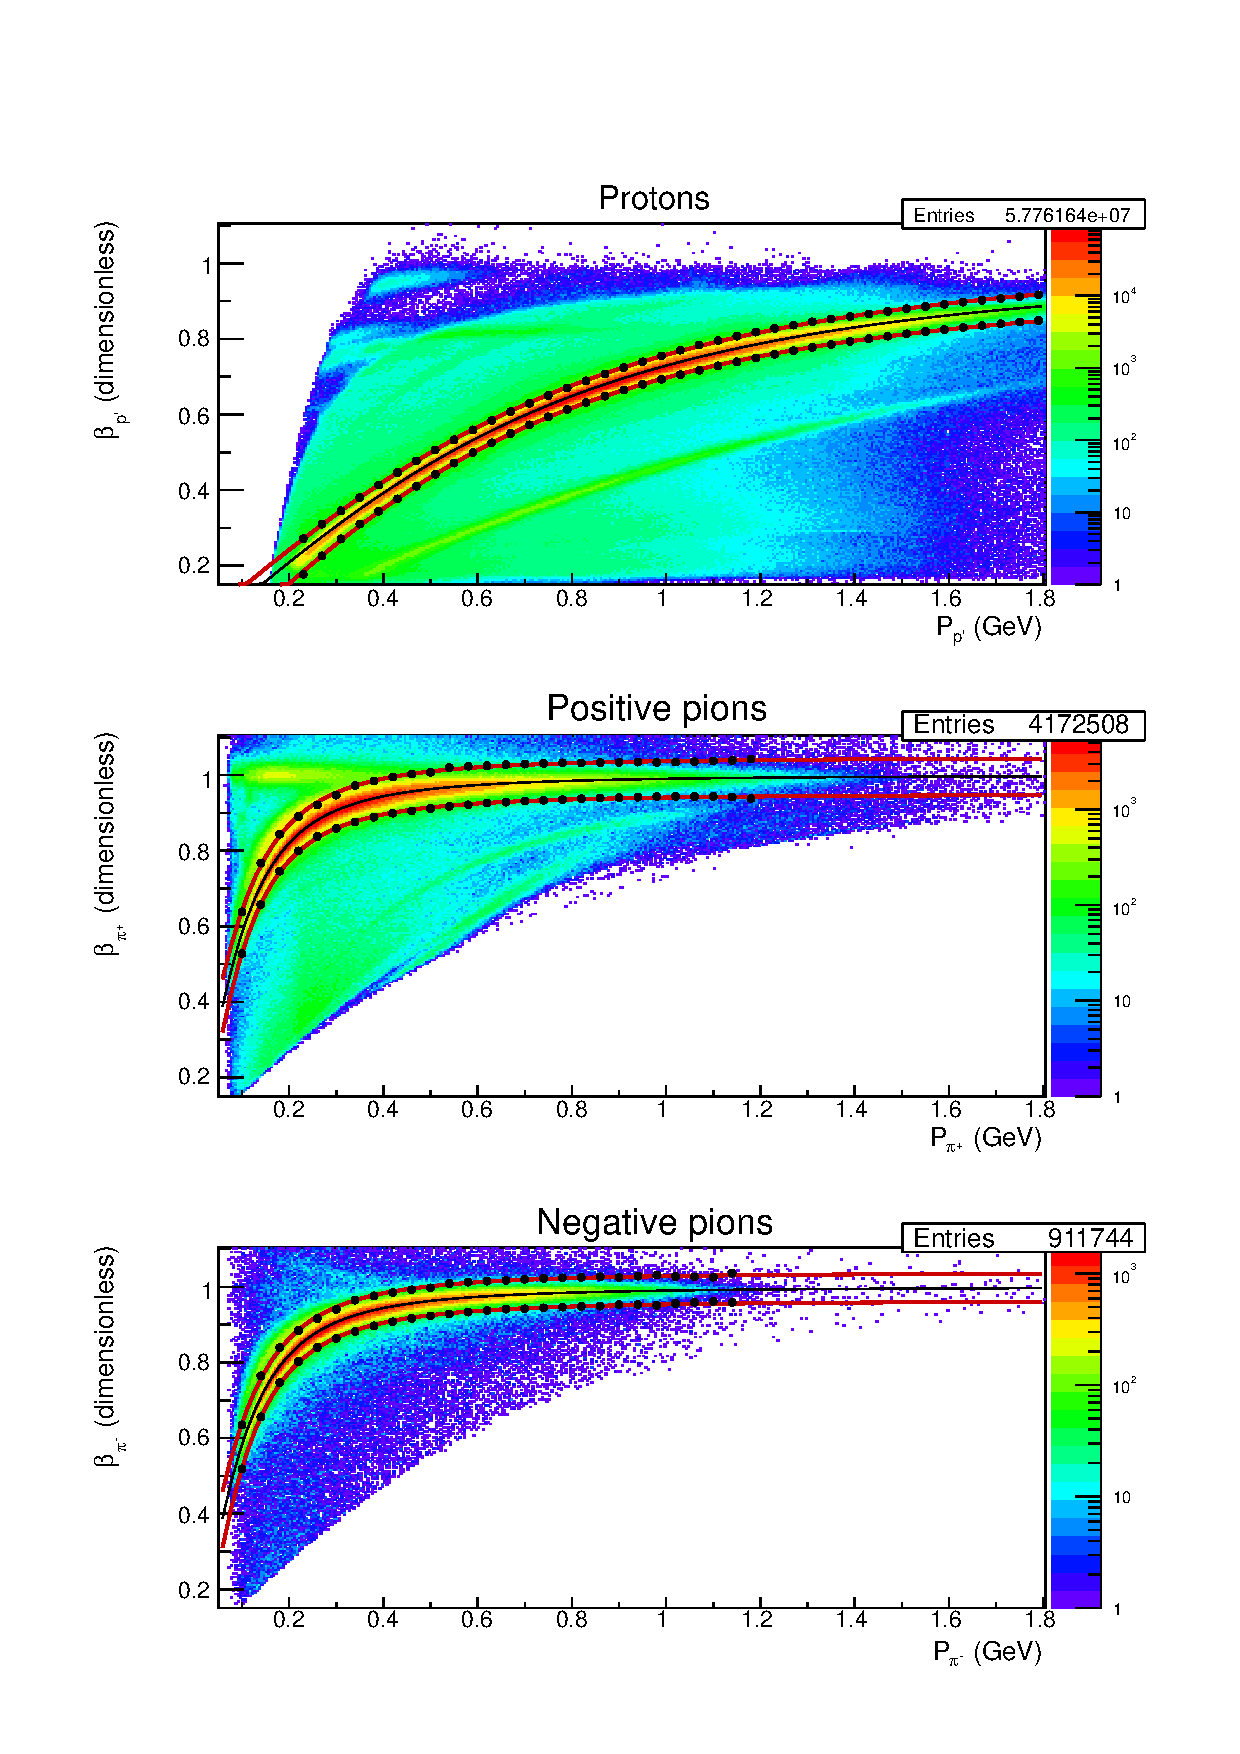
\includegraphics[width=14cm]{pictures/event_selection/hadron_id/hadron_id_cuts.pdf}}
\caption{\small $\beta_{corr}$ versus momentum distributions for proton (upper plot), positive pion (middle plot), and negative pion (bottom plot) candidates. Thin black solid curves in the middle of each band correspond to the nominal $\beta_{n}$ given by Eq.~\eqref{eq:hadron_hadronmass}. Black points correspond to the positions of Gaussian fit maxima $\pm 3\sigma$ for individual x-slices of the 2D histograms. These points are fit by the function Eq.~\eqref{eq:fit_f}, the resulting functions are shown by the red curves. Events between the red curves are selected for further analysis. \label{fig:hadron_id}} 
\end{center}
\end{figure}

Figure~\ref{fig:double_paddles} illustrates the timing correction for type C problematic paddles \#46 in sector 3 (left side) and \#40 in sector 5 (right side) for $\pi^+$ candidates. The plots in the first row clearly show the double band structures in $\beta_{h}$ versus momentum and $\Delta T$ versus momentum distributions. To perform timing correction for this type of paddles, one needs to determine the position $t_{shift}$ of each incorrect $\Delta T$-band (see horizontal red lines in Fig.~\ref{fig:double_paddles}) and then to move both of them to the correct position around zero, as demonstrated in the second row. The corrected value of $\beta$ is again calculated according to Eq.~\eqref{eq:beta_corr} with the only distinction, that events from different $\Delta T$-bands are treated separately and different $t_{shift}$ values are used for them.

The $\beta_{corr}$ versus momentum distributions are shown in the second row in Fig.~\ref{fig:double_paddles}. As seen in these plots, after the timing correction is applied $\beta_{corr}$ versus momentum bands demonstrate neither double band structures nor shifts from the black curves.


Figures~\ref{fig:shifted_paddles} and~\ref{fig:double_paddles} give examples of the timing correction for $\pi^+$ candidates. Similar corrections have also been performed for proton and $\pi^{-}$ candidates.


After the timing problems are eliminated in each TOF paddle, the hadron identification can be made. For the hadron identification, only events with good electron candidates that have been selected in the previous step are used. Figure~\ref{fig:hadron_id} shows $\beta_{corr}$ versus momentum distributions for each type of hadron candidate: protons (upper plot), positive pions (middle plot), and negative pions (bottom plot). These distributions include all sectors and all TOF paddles (with the exclusion of bad ones). The red curves show the corresponding hadron id cuts. These curves were obtained in the following way. Firstly, x-slices of the 2D histograms are fit by Gaussians. In this way points that correspond to the positions of the fit maxima $\pm 3\sigma$ are obtained\footnote[6]{Note that to establish the upper cut boundary for pions, the $3\sigma$ value was used only for $p_{\pi}>0.54$~GeV. For $p_{\pi}<0.54$~GeV different smaller values were used. This was done in order to better separate good pion candidates from the small upper band that is located very close to the pion band and most likely corresponds to muons.}. These points are shown by black bullets in Fig.~\ref{fig:hadron_id}. They determine the upper and lower boundaries for the cut. Finally, to obtain smooth curves, all points are fit by the following function,
\begin{equation}
f(p_{h})=\frac{a_{0}\cdot p_{h}}{\sqrt{a_{1}\cdot p_{h}^{2}+m_{h}^{2}+a_{2}}}+a_{3},
\label{eq:fit_f}
\end{equation}
where $p_{h}$ is the hadron momentum, $m_{h}$ hadron mass, and $a_{0}$, $a_{1}$, $a_{2}$, $a_{3}$ are fit parameters.

Events which are located between the red curves in Fig.~\ref{fig:hadron_id} are selected for further analysis and treated as good corresponding hadron candidates. It also needs to be mentioned that the distribution for positive pions was plotted only for events that already have a good proton candidate, and the distribution for negative pions was plotted only for events with good proton and positive pion candidates. Furthermore, in order to simplify the analysis process, all hadrons were preselected on an initial analysis step. The consequence of this preselection is the fact that distributions shown in Fig.~\ref{fig:hadron_id} contain areas that are not populated with events.

These established hadron id cuts are also applied to the reconstructed Monte Carlo events. 


\section{Momentum corrections}
\label{Sect:momcorr}

\subsection{Proton momentum correction (energy loss)}
\label{Sect:pr_en_loss}


While traveling through the detector and the target, the final state particles lose a part of their energy due to the interactions with the medium. Therefore, the measured particle momentum appears to be lower than the actual value. GSIM simulation of the CLAS detector correctly propagates particles  through the media and, therefore, the effect of the energy loss is included into the efficiency and does not impact the extracted cross sections. However, in order to avoid shifts in the distributions of some kinematic quantities (e.g. missing masses) from their expected values, an energy loss correction is applied to the proton momentum magnitude, since the low-energy protons are affected the most by energy loss in the materials. This correction is based on the GSIM simulation of the CLAS detector and is performed for both experimental and reconstructed Monte Carlo events.

\begin{figure}[htp]
\begin{center}
\framebox{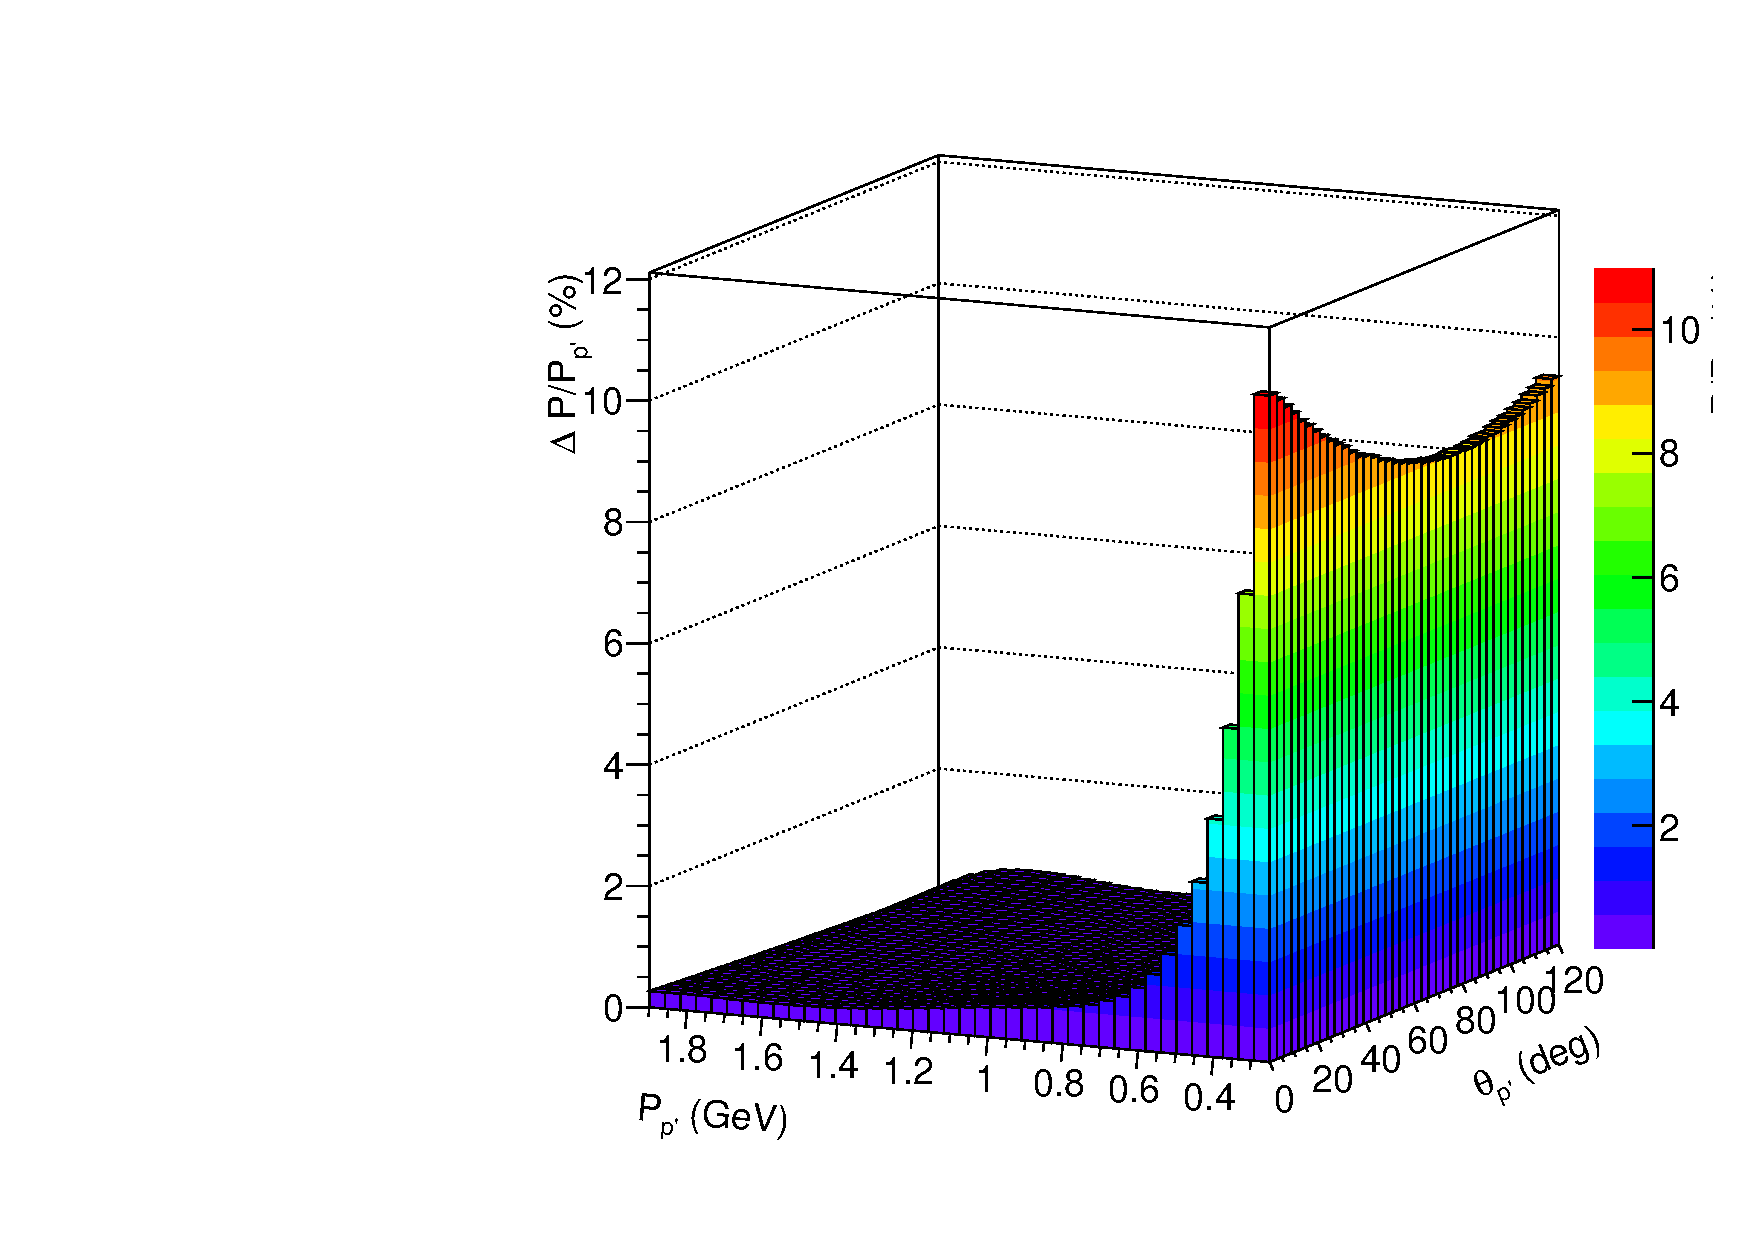
\includegraphics[width=8.75cm]{pictures/event_selection/mom_corr/eloss2d.pdf}}
\caption{\small Percentage of momentum that protons lose when they move through the detector and target media as a function of the momentum $P_{p'}$ and scattered angle $\theta_{p'}$ of the final proton. \label{fig:eloss}} 
\end{center}
\end{figure}

To obtain the correction function, the quantity $\Delta P$ that is the difference between the generated and reconstructed proton momenta was considered. This quantity was binned in the reconstructed proton momentum $P_{p'}$ and polar angle $\theta_{p'}$ and fit by a Gaussian in each $(P_{p'},~\theta_{p'})$ bin. The obtained mean values were further fit by a fifth order polynomial as a function of $P_{p'}$ in each $\theta_{p'}$ bin. Then the parameters of the resulting fit functions were fit as a function of $\theta_{p'}$ by a second order polynomial. 



The resulting energy loss correction function is shown in Fig.~\ref{fig:eloss}. It gives the percentage of the momentum that protons lose when they move through the detector and target media. %This function is used to correct the proton momentum both in the data and simulation.
%This function depends on $P_{p'}$ as a fifth order polynomial and has a quadratic dependence on $\theta_{p'}$.

Note that if one wants to isolate the pure effect of the energy loss, the difference between proton momenta for events reconstructed with and without detector and target materials must be considered. Since in the applied procedure the difference between generated and reconstructed proton momenta is analyzed, the correction function shown in Fig.~\ref{fig:eloss} can also include other effects that lead to improper proton momentum reconstruction.



\subsection{Electron momentum correction}
\label{Sect:el_momcor}

Due to slight misalignments in the DC position, small inaccuracies in the description of the torus magnetic field, and other possible reasons the momentum and angle of particles may have some small systematic deviations from their real values. These effects being of undefined origin cannot be simulated in GSIM, therefore a special momentum correction procedure is needed for the experimental data. According to~\cite{KPark:momcorr}, the evidence of the need for such corrections is most directly seen in the dependence of the elastic peak position on the azimuthal angle of the scattered electrons. It is shown in~\cite{KPark:momcorr} that the elastic peak position is shifted from the true value (0.938 GeV) and this shift is sector dependent.  

The significance of this effect depends on the beam energy. In the analysis~\cite{Fed_an_note:2017} it is shown that a beam energy of 2.039 GeV leads to the small shift ($\sim$ 3 MeV) in elastic peak position, while the study~\cite{KPark:momcorr} demonstrates that in case of  5.754 GeV beam energy this shift reaches 20 MeV. Moreover, the study~\cite{KPark:momcorr} also shows that this effect becomes discernible only if the particle momentum is sufficiently high (e.g. for pions the correction is needed only if their momentum is higher than 2 GeV). Thus, the small beam energy of this analyzed dataset and the fact that in double-pion kinematics hadrons carry only a small portion of the total momentum allows us to come to the conclusion that the correction is needed only for electrons, while deviation in hadron momenta can be neglected.

\begin{figure}[htp]
\begin{center}
\framebox{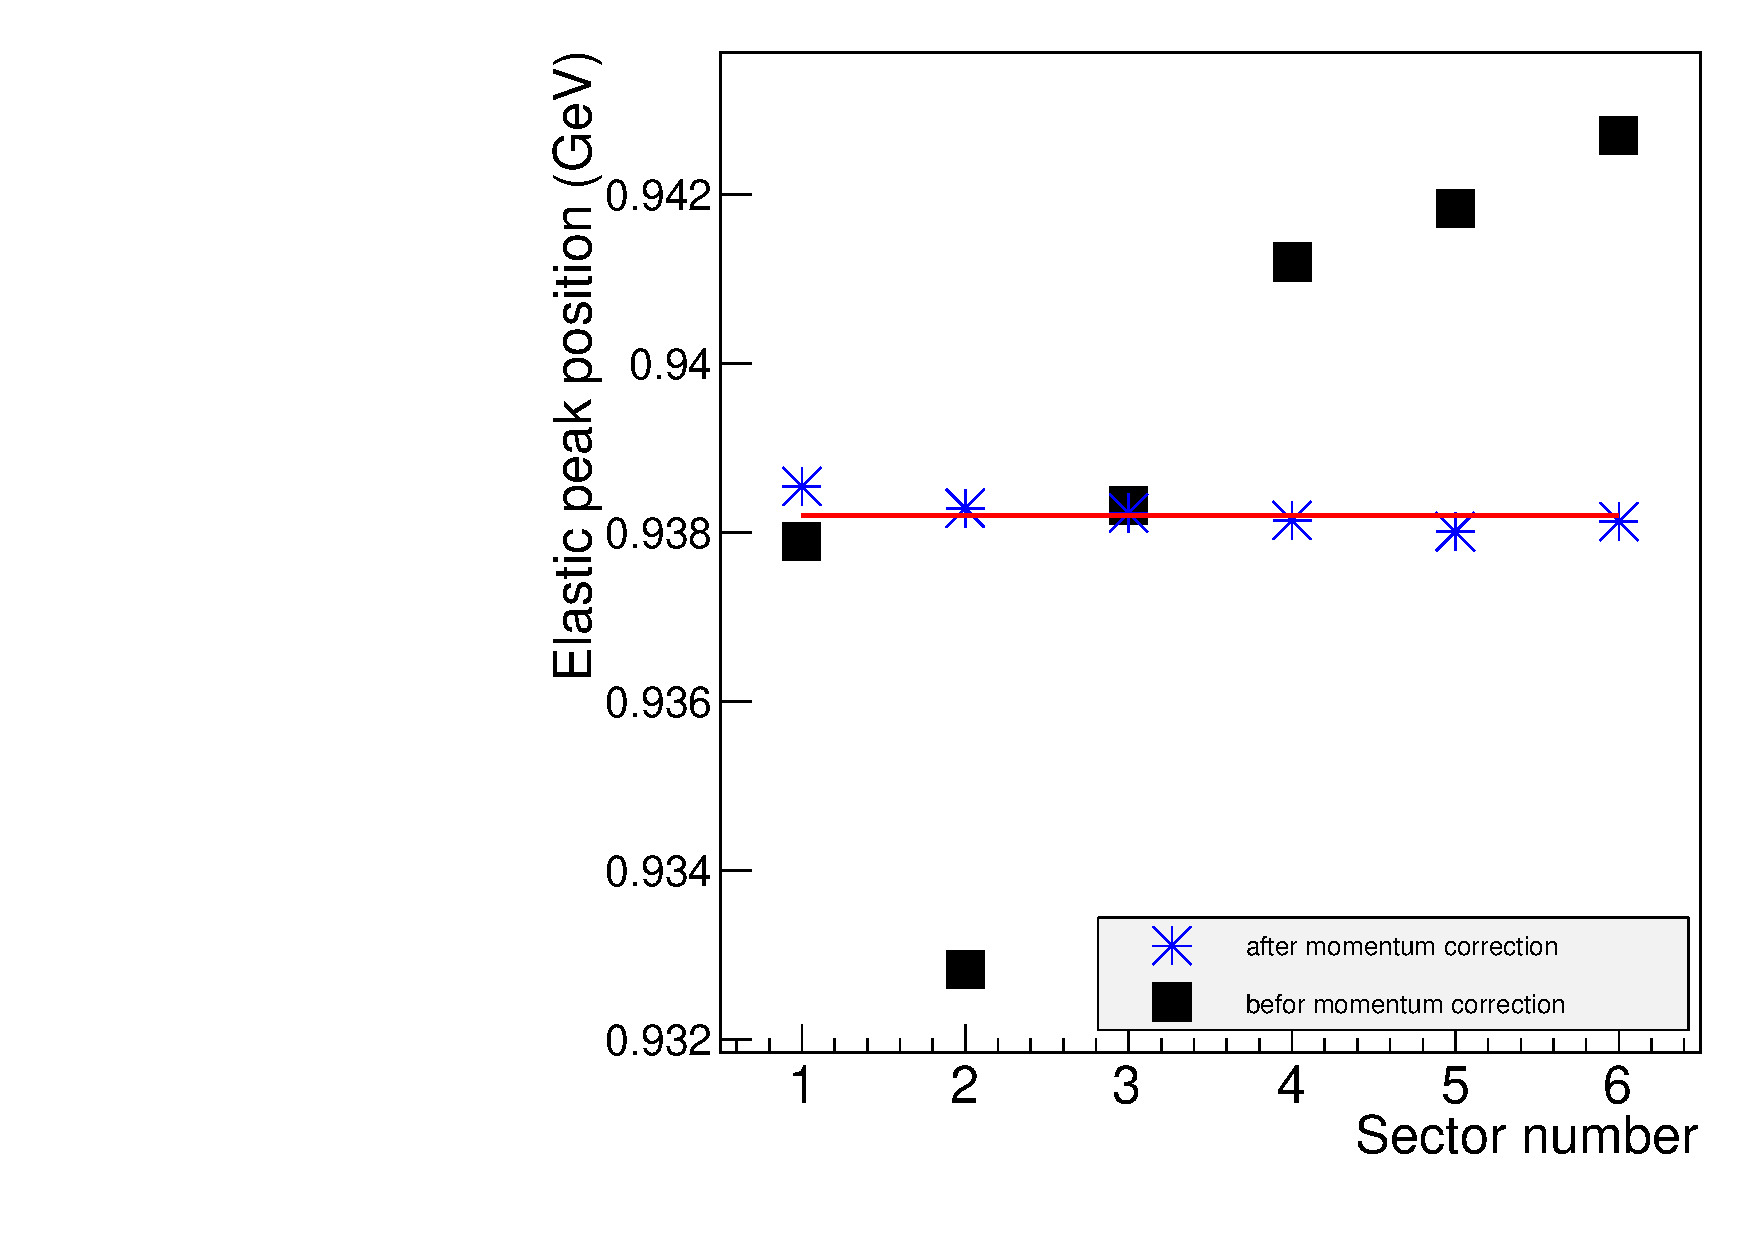
\includegraphics[width=7cm]{pictures/event_selection/mom_corr/elast_pic_position.pdf}}
\caption{\small Elastic peak position for the six CLAS sectors before (black squares) and after (blue stars) electron momentum correction for the proton part of ``e1e" dataset. The horizontal red line shows the proton mass. This figure is taken from the analysis~\cite{Fed_an_note:2017}. \label{fig:el_mom_corr_peak_position}} 
\end{center}
\end{figure}

Since this analysis suffers from additional complications as binding and motion of the target proton inside the deuteron, it was considered sensible to use the electron momentum corrections that have previously been developed and tested in the analysis of the free proton part of ``e1e" dataset at the same beam energy~\cite{Fed_an_note:2017}. To establish them, the approach~\cite{KPark:momcorr}, which is based on elastic kinematics, was used. These corrections include electron momentum magnitude correction as well as electron polar angle correction, which were developed for each CLAS sector individually.  


Figure~\ref{fig:el_mom_corr_peak_position}, which was taken from the analysis~\cite{Fed_an_note:2017}, demonstrates that after the electron momentum corrections the elastic peak position for all CLAS sectors gets closer to the proton mass, shown by the red horizontal line.

\begin{figure}[htp]
\begin{center}
\framebox{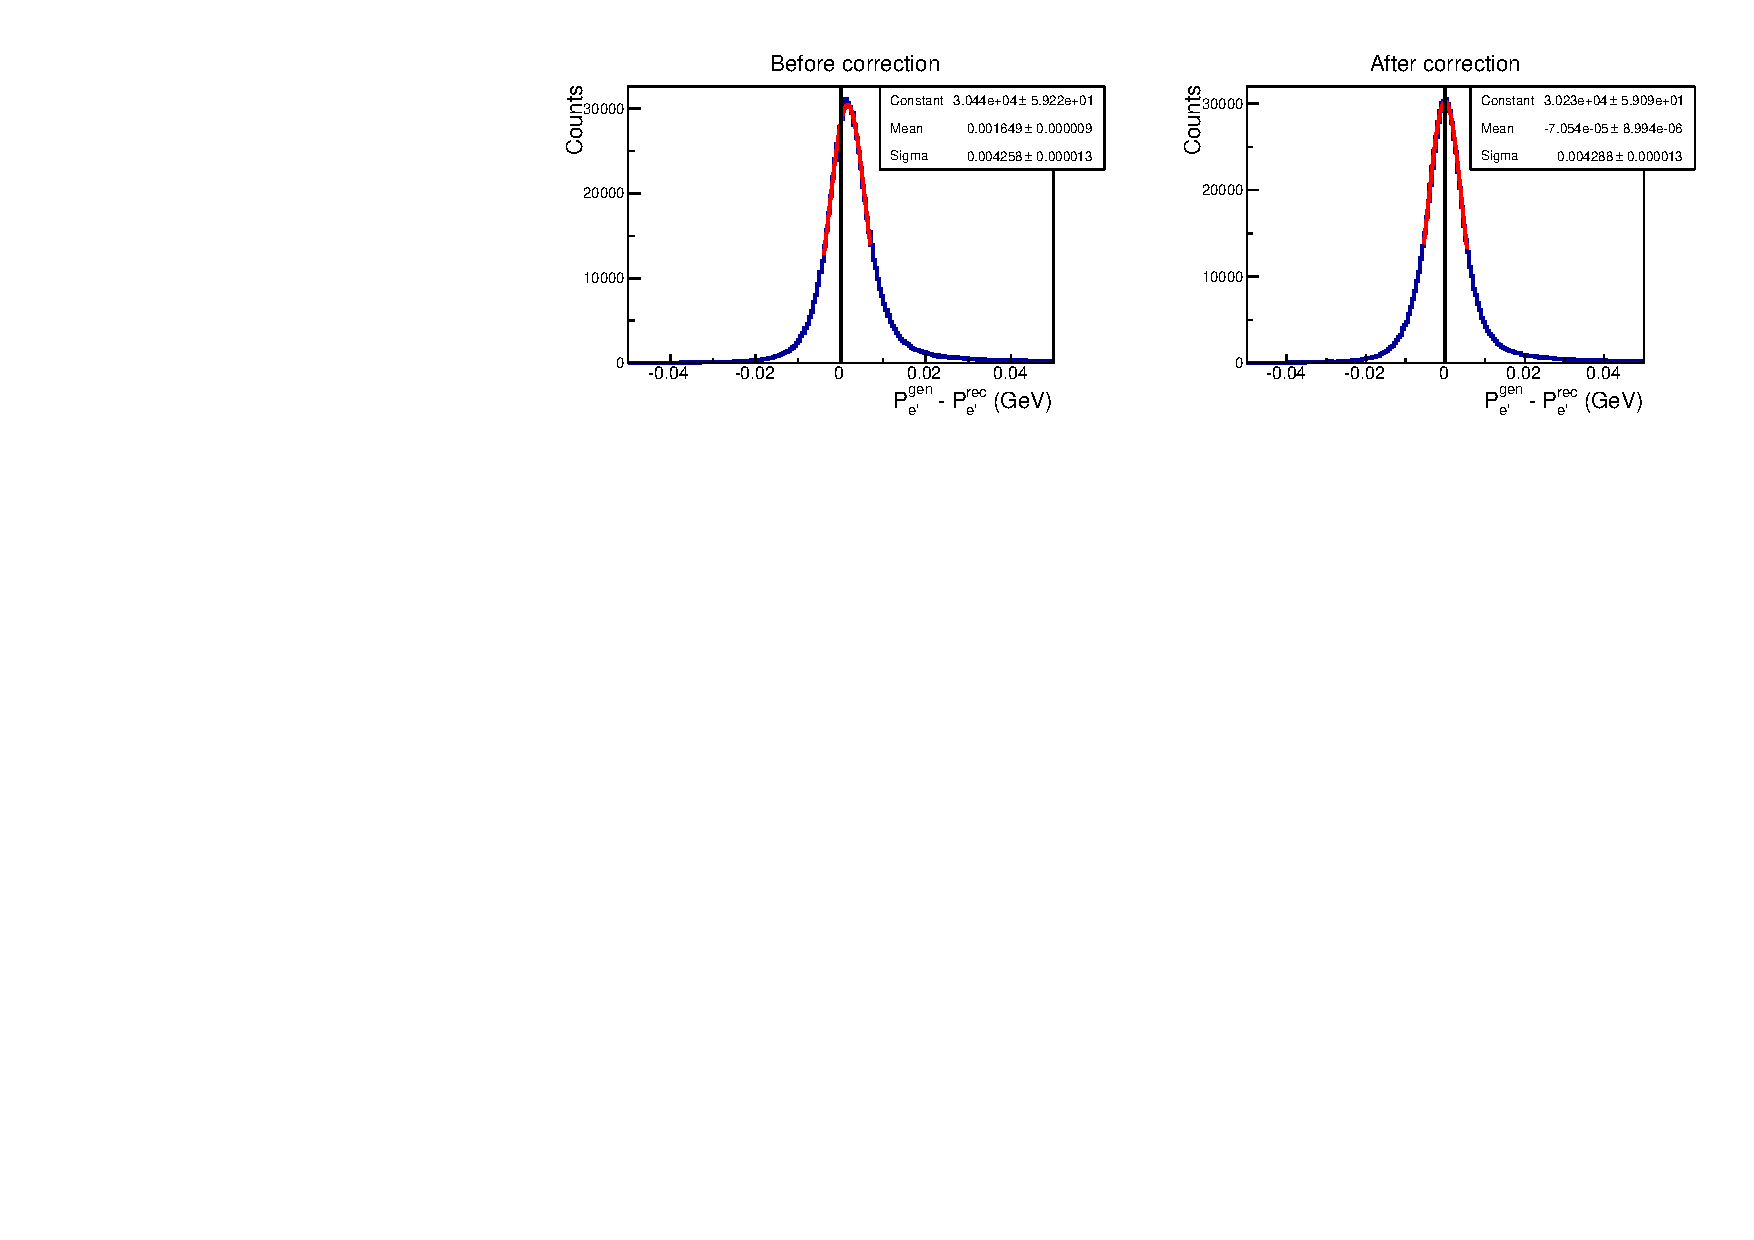
\includegraphics[width=14cm]{pictures/event_selection/mom_corr/el_sim_momcor_bef_aft.pdf}}
\caption{\small Difference between generated and reconstructed electron momenta before (left plot) and after (right plot) the correction of the momentum magnitude, which has been applied to the reconstructed electrons. The vertical black line shows the position of zero. \label{fig:el_mom_corr_sim}} 
\end{center}
\end{figure}

The correction discussed above is applied only for experimental data. As for the Monte Carlo simulation, it turns out that due to unknown reasons (most likely because electrons lose some energy when they travel through the detector and target media) the reconstructed electron momentum appears to be slightly lower than the generated one. This effect is demonstrated in the left plot of Fig.~\ref{fig:el_mom_corr_sim}, where the event distribution of the quantity $\Delta P$ (which is the difference between generated and reconstructed electron momenta) is presented. Therefore, an adapted procedure of correcting the electron momentum magnitude is also applied to the reconstructed Monte Carlo events. This procedure is similar to that used for the proton energy loss (see Sect.~\ref{Sect:pr_en_loss}). The correction depends only on the scattered electron momentum and polar angle, but not on the CLAS sector. The typical value of this correction is 0.2\%. The right plot in Fig.~\ref{fig:el_mom_corr_sim} shows the result of the correction. As seen in this plot, the mean value of the quantity $\Delta P$ demonstrates no shift from zero when the momentum magnitude for reconstructed electron is corrected. 


\section{Other cuts}
\label{Sect:other_cuts}


\subsection{Fiducial cuts}
\label{Sect:fiduc} 

The active detection solid angle of the CLAS detector is smaller than $4\pi$~\cite{Mecking:2003zu}. This is in part due to the space filled with the torus field coils: the angles covered by the coils are not equipped with any detection system and therefore form a ``dead" area for detection. Additionally, the detection area is also limited in polar angle from 8$^{\circ}\mathrm{}$ up to 45$^{\circ}\mathrm{}$ for electrons and up to 140$^{\circ}\mathrm{}$ for other charged particles~\cite{Mecking:2003zu}. Moreover, different studies and analyses have shown that also the edges of the active area do not provide a safe region for the particle reconstruction, being affected by rescattering from the coil, field distortions, and similar effects. Therefore, it is now common practice to accept for the analysis only events inside specific fiducial cuts, i.e. cuts on the kinematic variables (momentum and angles) of each particle. This method guarantees that events accepted in the analysis include only particles detected in ``safe" areas of the detector, where the acceptance is thought to be well understood. These cuts are applied to both real events and reconstructed Monte Carlo events. 


\subsubsection{Fiducial cuts for negatively charged particles}
\label{Sect:fiduc_neg}

In CLAS experiments with normal direction of the torus magnetic field, like in the ``e1e" experiment, negatively charged particles are inbending, which means that their trajectories are bent in the forward direction. For these particles sector independent, symmetrical, and momentum dependent cuts are applied. 

For electron and negative pion candidates the analytical shapes of fiducial cuts are given by Eq.~\eqref{eq:fiduch_electrons} and Eq.~\eqref{eq:fiduch_pim}, respectively. The shapes of these cuts were taken from the similar analysis~\cite{Fed_an_note:2017} of the ``e1e" dataset (but off proton target) and carefully adjusted to the data.

In Eq.~\eqref{eq:fiduch_electrons} and Eq.~\eqref{eq:fiduch_pim} polar and azimuthal angles of electrons $(\theta_{e'},~\varphi_{e'})$ and negative pions $(\theta_{\pi},~\varphi_{\pi})$ are assumed to be in degrees, while their momenta $(p_{e'},~p_{\pi})$ are in GeV, respectively. The angles are taken at the interaction vertex. Events that satisfy the criteria $\theta^{min} < \theta < \theta^{max}$ and $\varphi^{min} < \varphi < \varphi^{max}$ are selected for the analysis. 
\clearpage


\begin{equation}
\begin{aligned}
& \theta_{e'}^{min}(p_{e'})  & = &~11.7398+\frac{8.21504}{0.433327\cdot p_{e'}+0.158076}. \\[8pt]
& \theta_{e'}^{max}(p_{e'}) & = &~76.8617 -76.537\cdot p_{e'} + 77.9387\cdot p_{e'}^{2}-28.389\cdot p_{e'}^{3}.\\[8pt]
& \varphi_{e'}^{min}(\theta_{e'})  & = &~-41.3\!\cdot\! \sin\left [ a_{3}\cdot (\theta_{e'}-\theta_{e'}^{min}) \right ]^{\left [a_{1}+a_{2}/\theta_{e'}+1485/\theta_{e'}^{2}\right ]} -1.  \\[8pt]
& \varphi_{e'}^{max}(\theta_{e'})  & = &~+41.3\!\cdot\! \sin\left [ a_{3}\cdot (\theta_{e'}-\theta_{e'}^{min}) \right ]^{\left [a_{1}+a_{2}/\theta_{e'}+1485/\theta_{e'}^{2} \right ]}+1. \\[8pt]
& a_{1}(p_{e'})& = &~0.85+1.1\cdot p_{e'}.\\[8pt]
& a_{2}(p_{e'})& = &~-62.8-30\cdot p_{e'}.\\[8pt]
& a_{3}(p_{e'})& = &~ 0.0047\cdot p_{e'} + 0.0079.\\
\end{aligned} \label{eq:fiduch_electrons} 
\end{equation}

\vspace{2em}

\begin{equation}
\begin{aligned}
& \theta_{\pi}^{min}(p_{\pi})  & = &~10.09+\frac{8}{0.472\cdot (p_{\pi}-0.03)+0.117},~\textrm{if}~p_{\pi}>0.3. \\[8pt]
& \theta_{\pi}^{min2}(p_{\pi})  & = &~33 +\frac{5.24894\cdot 10^{-5}}{5.71075\cdot 10^{-5}\cdot(p_{\pi}+0.004)^{2}},~\textrm{if}~p_{\pi}<0.3. \\[8pt]
& \theta_{\pi}^{max} & = &~140. \\[8pt]
& \varphi_{\pi}^{min}(\theta_{\pi})  & = & \begin{sqcases} 
-23.5\!\cdot\! \sin\left [ 0.015\cdot (\theta_{\pi}-\theta_{\pi}^{min}) \right ] ^{\left [a_{1}+a_{2}/\theta_{\pi}+1400/\theta_{\pi}^{2}\right ]}-a_{3},&\textrm{if}~\theta_{\pi}<\theta_{\pi}^{*}\\ 
 \varphi_{\pi}^{min}(\theta_{\pi}^{*}),&\textrm{if}~\theta_{\pi}>\theta_{\pi}^{*} \\[8pt]
\end{sqcases}. \\
& \varphi_{\pi}^{max}(\theta_{\pi})  & = & \begin{sqcases} 
+23.5\!\cdot\! \sin\left [ 0.015\cdot (\theta_{\pi}-\theta_{\pi}^{min}) \right ] ^{\left [a_{1}+a_{2}/\theta_{\pi}+1400/\theta_{\pi}^{2}\right ]}+a_{3},&\textrm{if}~\theta_{\pi}<\theta_{\pi}^{*}\\ 
 \varphi_{\pi}^{max}(\theta_{\pi}^{*}),&\textrm{if}~\theta_{\pi}>\theta_{\pi}^{*} \\[8pt]
\end{sqcases}. \\
& a_{1}(p_{\pi}) & = &~0.61+1.18\cdot p_{\pi}.\\[8pt]
& a_{2}(p_{\pi}) & = &~-59.2-35.3\cdot p_{\pi}.\\[8pt]
& a_{3}(p_{\pi}) & = &~17.2\cdot p_{\pi}-11.9\cdot p_{\pi}^{2}-2.5.\\[8pt]
& \theta_{\pi}^{*} & = &~\theta_{\pi}^{max}- \frac{13}{15}\cdot(\theta_{\pi}^{max}-\theta_{\pi}^{min}).\\
\end{aligned} \label{eq:fiduch_pim} 
\end{equation}
\clearpage

\begin{figure}[htp]
\begin{center}
\framebox{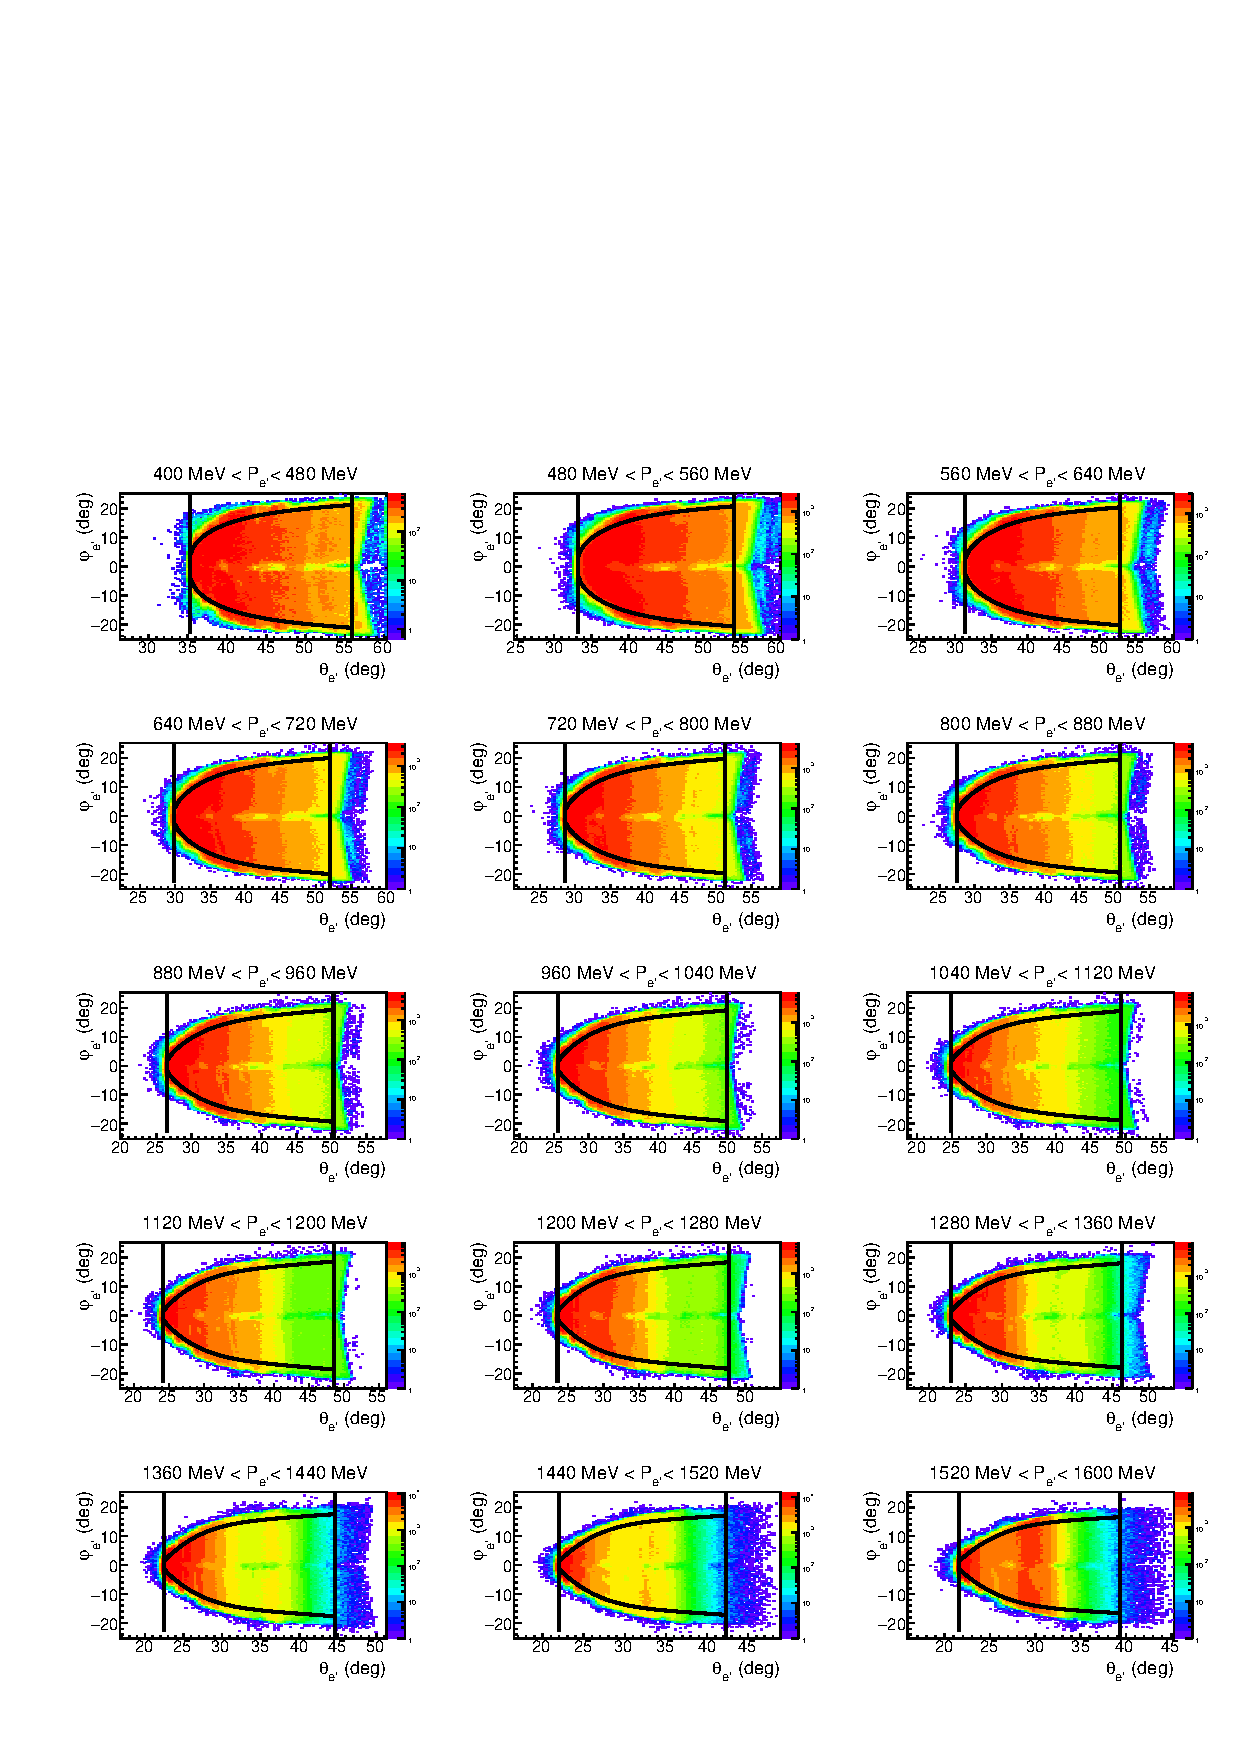
\includegraphics[width=15.cm]{pictures/other_cuts/fiducial/el_fid_2dim_mom_slice_fin.pdf}}
\caption{\small $\varphi$ versus $\theta$ distributions for electron candidates for different 80-MeV-wide momentum slices plotted for events from all CLAS sectors. Curves show the applied fiducial cuts given by Eq.~\eqref{eq:fiduch_electrons}, vertical lines stand for $\theta_{e'}^{min}$ and $\theta_{e'}^{max}$. The angles are taken at the interaction vertex. For each momentum slice the shape of the fiducial cut was calculated for the value of the electron momentum taken in the center of the momentum bin.  \label{fig:fiduch_el_2d}}
\end{center}
\end{figure}

\clearpage

\begin{figure}[htp]
\begin{center}
\framebox{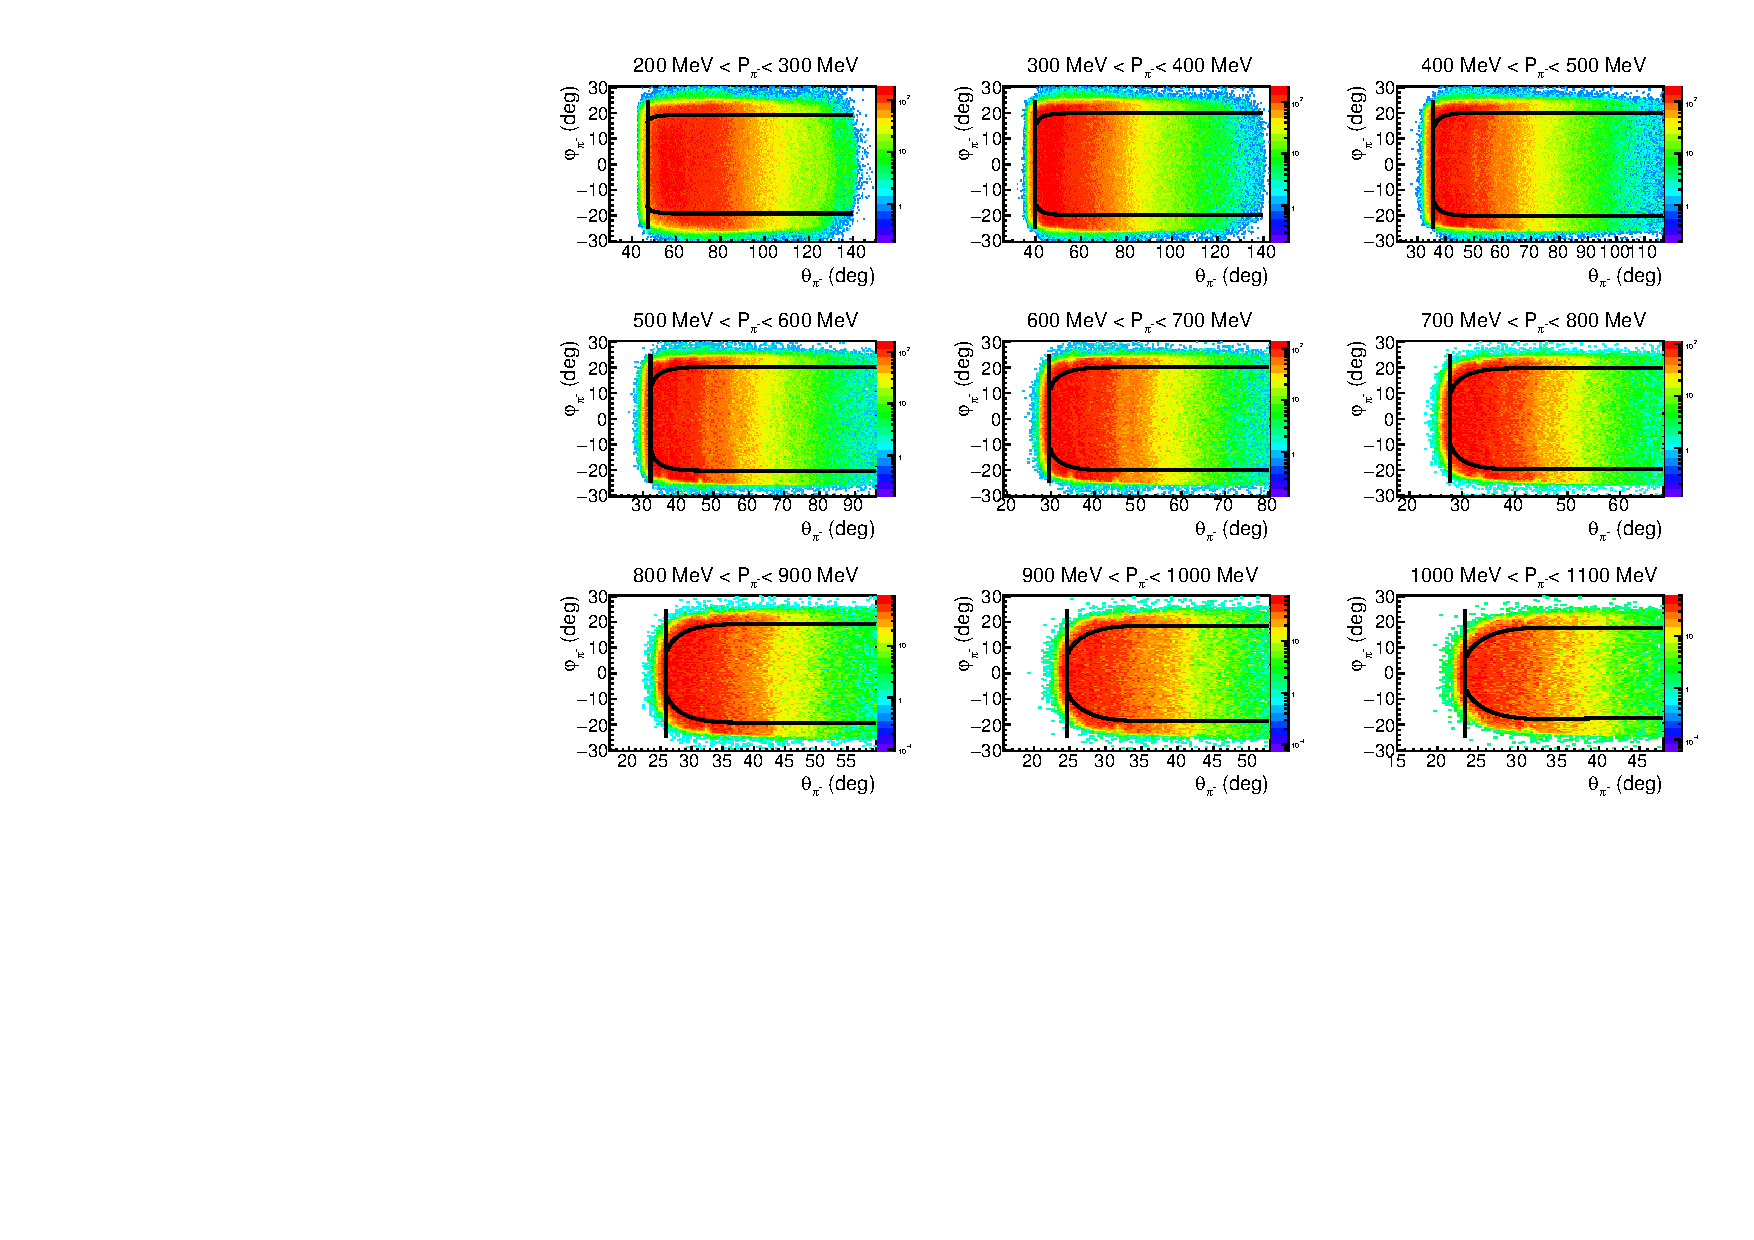
\includegraphics[width=15.cm]{pictures/other_cuts/fiducial/pim_fid_2dim_mom_slice.pdf}}
\caption{\small $\varphi$ versus $\theta$ distributions for negative pion candidates for different 100-MeV-wide momentum slices plotted for events from all CLAS sectors. Curves show the applied fiducial cuts given by Eq.~\eqref{eq:fiduch_pim}, vertical lines stand for $\theta_{\pi}^{min}$ and $\theta_{\pi}^{max}$. The angles are taken at the interaction vertex. For each momentum slice the shape of the fiducial cut was calculated for the value of the pion momentum taken in the center of the momentum bin. \label{fig:fiduch_pim_2d}}
\end{center}
\end{figure}


The fiducial cut for electron candidates is illustrated in Fig.~\ref{fig:fiduch_el_2d}, where the curves given by Eq.~\eqref{eq:fiduch_electrons} are superimposed on the $\varphi$ versus $\theta$ distributions for different 80-MeV-wide momentum slices. Vertical lines correspond to $\theta_{e'}^{min}$ and $\theta_{e'}^{max}$. For each momentum slice the shape of the fiducial cut was calculated for the value of the electron momentum taken in the center of the momentum bin. The depleted area around $\varphi_{e'} = 0$ corresponds to the inefficient region in CC and was discussed above in Sect.~\ref{Sect:cc_cuts}.  

The fiducial cut for negative pion candidates is illustrated in Fig.~\ref{fig:fiduch_pim_2d}, where the curves given by Eq.~\eqref{eq:fiduch_pim} are superimposed on the $\varphi$ versus $\theta$ distributions for different 100-MeV-wide momentum slices. Vertical lines correspond to $\theta_{\pi}^{min}$ and $\theta_{\pi}^{max}$. For each momentum slice the shape of the fiducial cut was calculated for the value of the pion momentum taken in the center of the momentum bin.

The same fiducial cuts for negatively charged particles are also applied to the reconstructed Monte Carlo events.
\clearpage

\begin{figure}[htp]
\begin{center}
\framebox{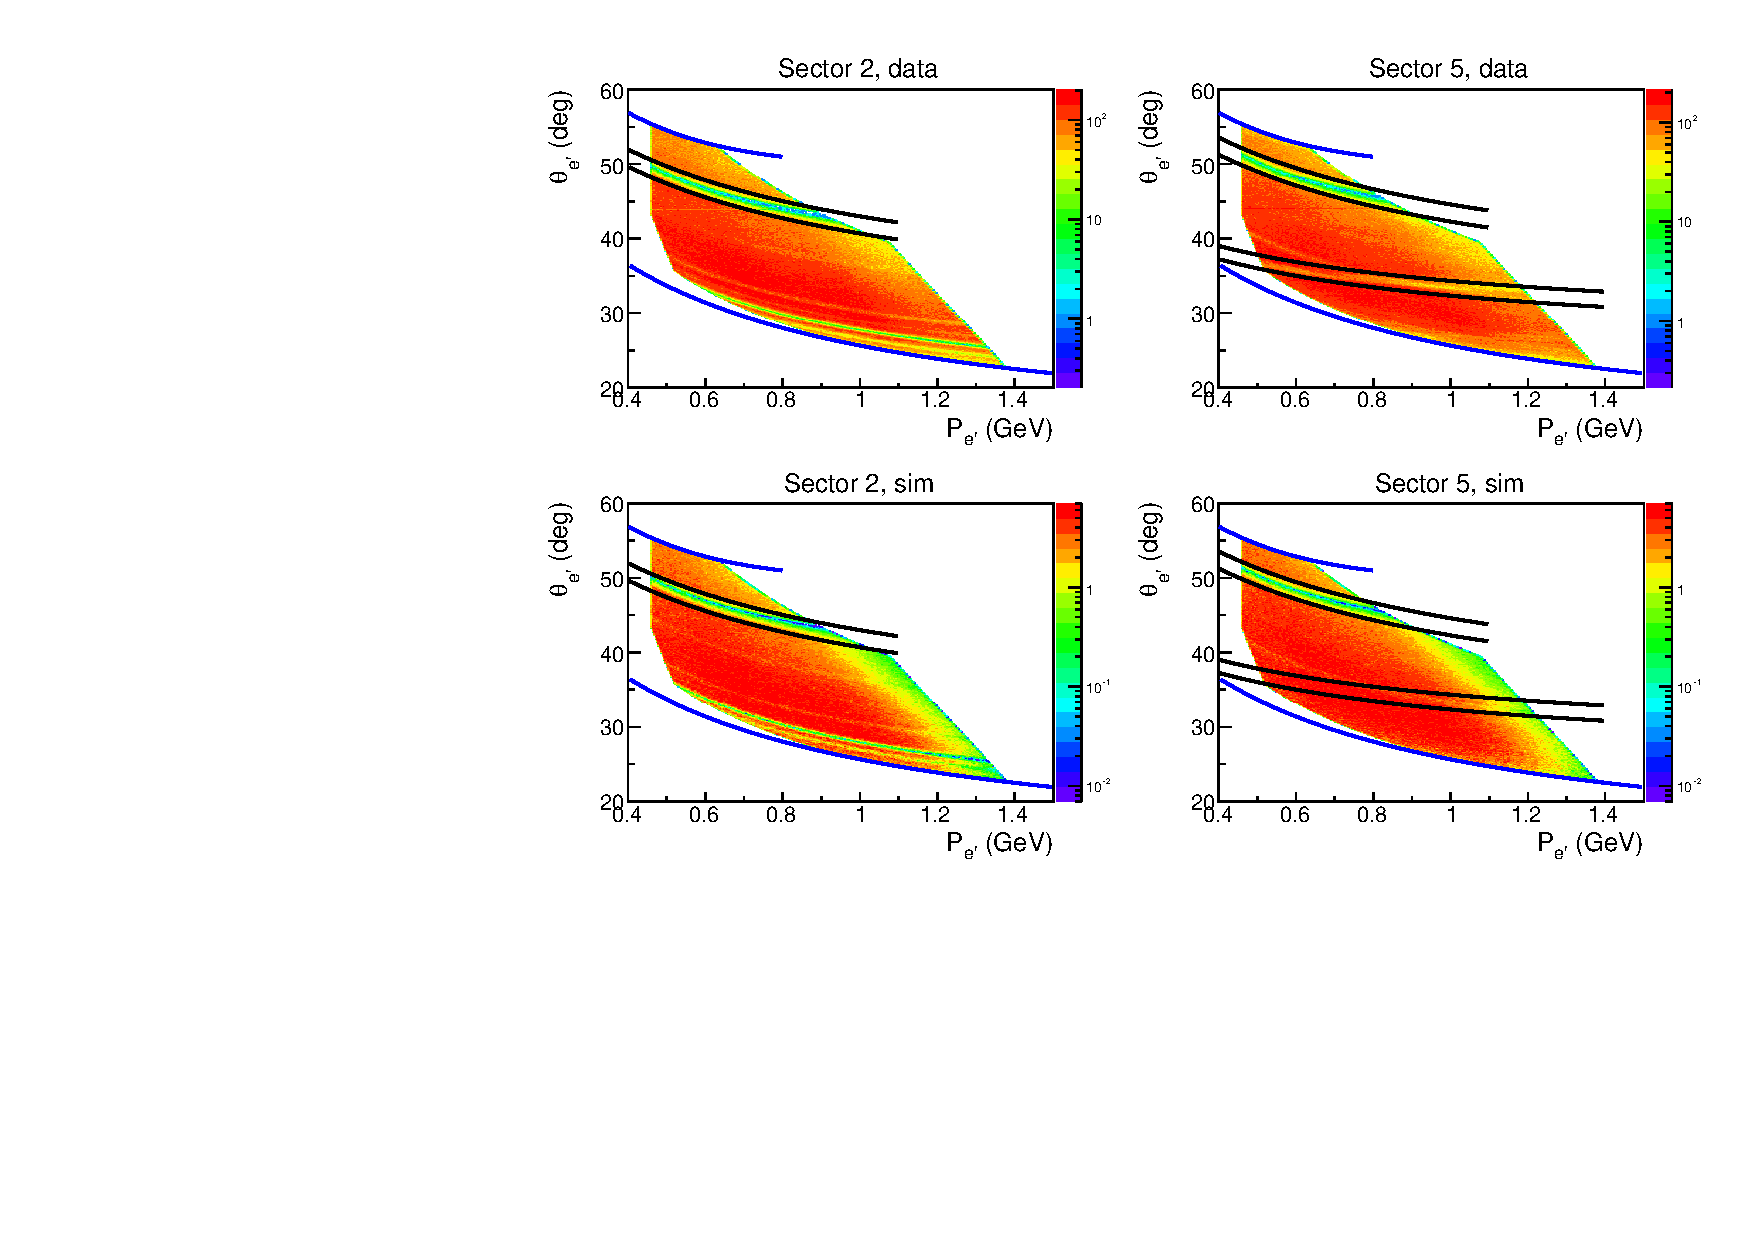
\includegraphics[width=9.cm]{pictures/other_cuts/fiducial/th_vs_p_el_new.pdf}}
\caption{\small  $\theta$ versus momentum distributions for electron candidates for CLAS sectors two (left side) and five (right side). The angle $\theta$ is taken at the interaction vertex. Top row corresponds to the data, bottom row corresponds to the reconstructed Monte Carlo events. Blue curves correspond to $\theta_{e'}^{min}$ and $\theta_{e'}^{max}$ in Eq.~\eqref{eq:fiduch_electrons}. Black curves correspond to additional fiducial $\theta$ versus momentum cuts. These distributions are plotted under the conditions 1.3~GeV $< W <$ 1.825~GeV and 0.4~GeV$^{2}$ $< Q^{2} <$ 1.0~GeV$^{2}$ which account for the extra cuts of the distribution edges. Other small inefficiencies that are seen in these plots are due to the geometrical cut in the CC plane (see Sect.~\ref{Sect:cc_cuts}). \label{fig:th_vs_p_el}}
\end{center}
\end{figure}

There are some additional dead areas in CLAS acceptance that are not related to the gaps between the sectors and limitations on the detection polar angle. They are typically caused by some inefficiencies in the Drift Chambers and Time-of-Flight system (dead wires or PMTs). Some of them are well reproduced in the Monte Carlo simulation, while others are not. To exclude the latter from the analysis and to eliminate events near the acceptance edges, additional fiducial cuts on $\theta$ versus momentum distributions are applied. These cuts are individual for each CLAS sector. They are shown by the black curves for real and Monte Carlo events in Fig.~\ref{fig:th_vs_p_el} for electron candidates and in Fig.~\ref{fig:th_vs_p_pim} for negative pion candidates. 

For the electron distributions shown in Fig.~\ref{fig:th_vs_p_el} inefficient areas in sectors two and five correspond to bad TOF paddles \#16 and \#17, respectively. Other small inefficiencies that are seen in these plots are due to the geometrical cut in the CC plane (see Sect.~\ref{Sect:cc_cuts}), they are almost identical for data and Monte Carlo events and, therefore, no additional fiducial cuts are needed for them.  $\theta$ versus momentum distributions for electron candidates in other sectors do not show significant inefficiencies. 


\begin{figure}[htp]
\begin{center}
\framebox{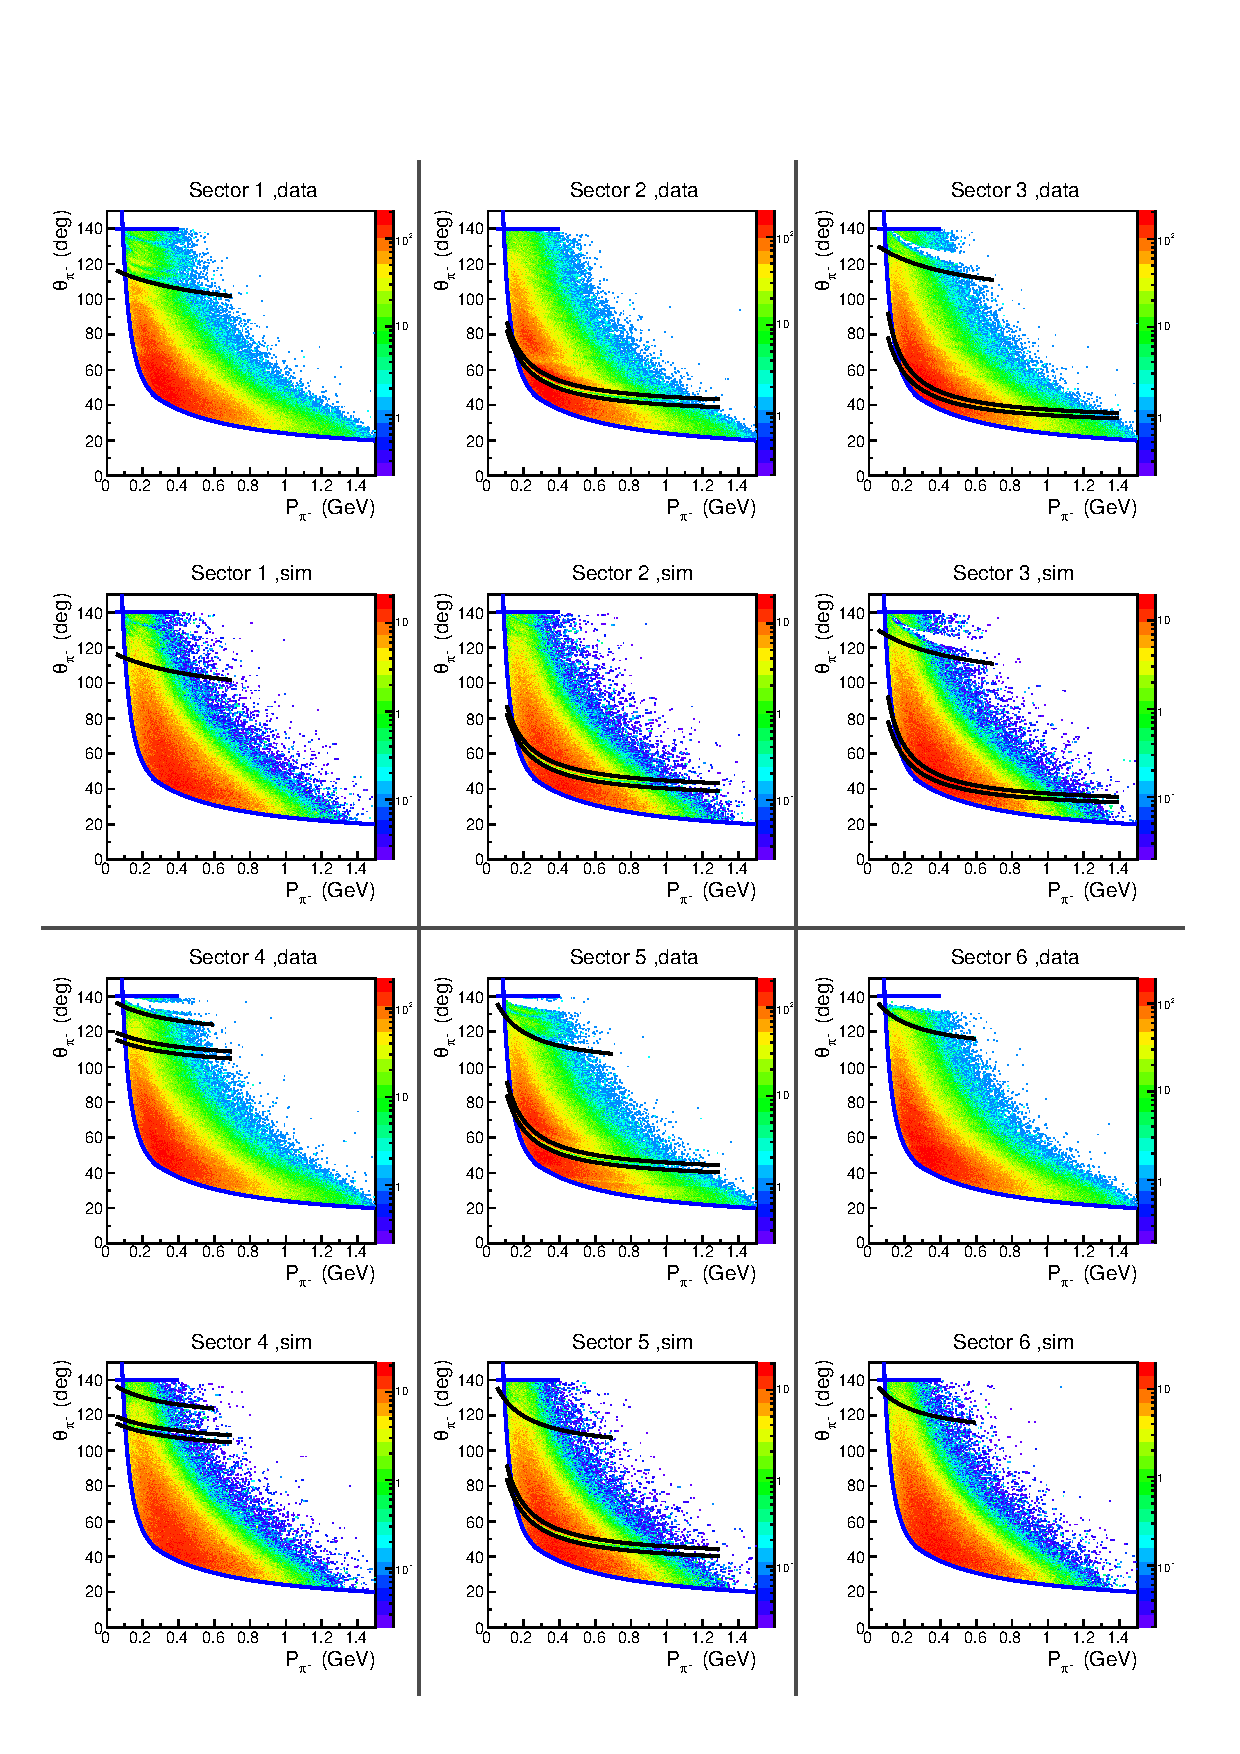
\includegraphics[width=14.5cm]{pictures/other_cuts/fiducial/th_vs_p_pim2.pdf}}
\caption{\small $\theta$ versus momentum distributions for negative pion candidates for different CLAS sectors. The angle $\theta$ is taken at the interaction vertex. Plots are given both for real data and reconstructed Monte Carlo events. Blue curves correspond to $\theta_{\pi}^{min}$ and $\theta_{\pi}^{max}$ in Eq.~\eqref{eq:fiduch_pim}. Black curves correspond to additional fiducial $\theta$ versus momentum cuts. \label{fig:th_vs_p_pim}}
\end{center}
\end{figure}

\clearpage
\subsubsection{Fiducial cuts for positively charged particles}
\label{Sect:fiduc_pos}

For positively charged particles, which are outbending in the ``e1e" experiment, momentum independent and symmetrical fiducial cuts suit our purpose best. The analytical shape of these cuts is given by Eq.~\eqref{eq:fiduch_pos}, which was also taken from the analysis~\cite{Fed_an_note:2017} and carefully adjusted to the data. All angles in Eq.~\eqref{eq:fiduch_pos} are taken at the interaction vertex and assumed to be in degrees. Events that satisfy the criteria $\theta^{min} < \theta < \theta^{max}$ and $\varphi^{min} < \varphi < \varphi^{max}$ are selected for the analysis. 

\begin{equation}
\begin{aligned}
&  \theta^{min} & = &~12.\\[8pt]
&  \theta^{max} & = &  \begin{sqcases} 
60&\textrm{for~protons} \\ 
120&\textrm{for~pions}\\[2pt]
\end{sqcases}. \\
& \varphi^{min}(\theta)  & = &~-25\!\cdot\! \left [1-e^{\left [-0.12\cdot (\theta-10)\right ]}\right ]+3.  \\[8pt]
& \varphi^{max}(\theta)  & = &~+25\!\cdot\! \left [1-e^{\left [-0.12\cdot (\theta-10)\right ]}\right ]-3. \\[8pt]
\end{aligned} \label{eq:fiduch_pos} 
\end{equation}

Fiducial cuts for positive hadron candidates are illustrated in Fig.~\ref{fig:fiduch_pos_2d}, where the curves given by Eq.~\eqref{eq:fiduch_pos} are superimposed on the $\varphi$ versus $\theta$ distributions for protons (left plot) and pions (right plot). Vertical lines correspond to $\theta^{min}$ and $\theta^{max}$. The same fiducial cuts for positively charged particles are also applied to the reconstructed Monte Carlo events.


\begin{figure}[!ht]
\begin{center}
\framebox{
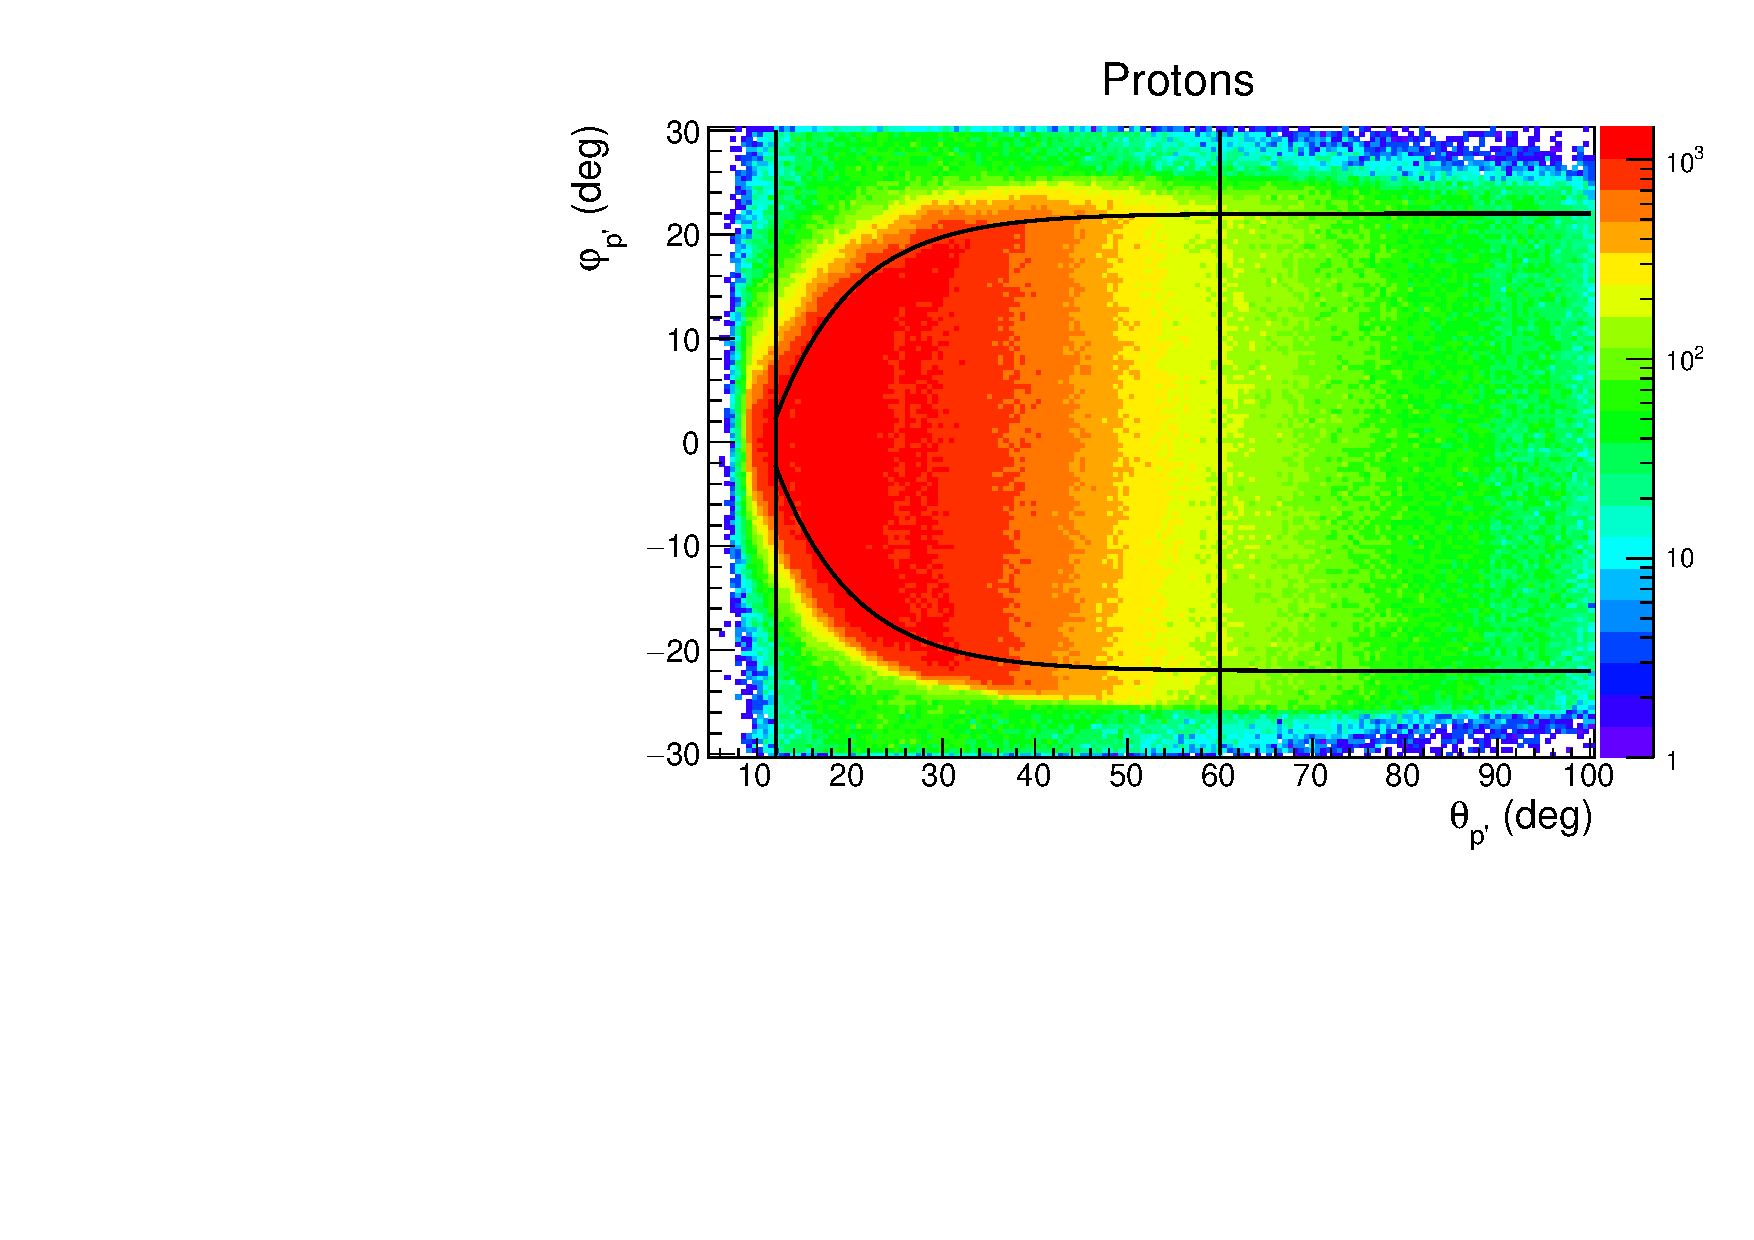
\includegraphics[width=0.4\textwidth]{pictures/other_cuts/fiducial/fid_p_2dim.pdf}
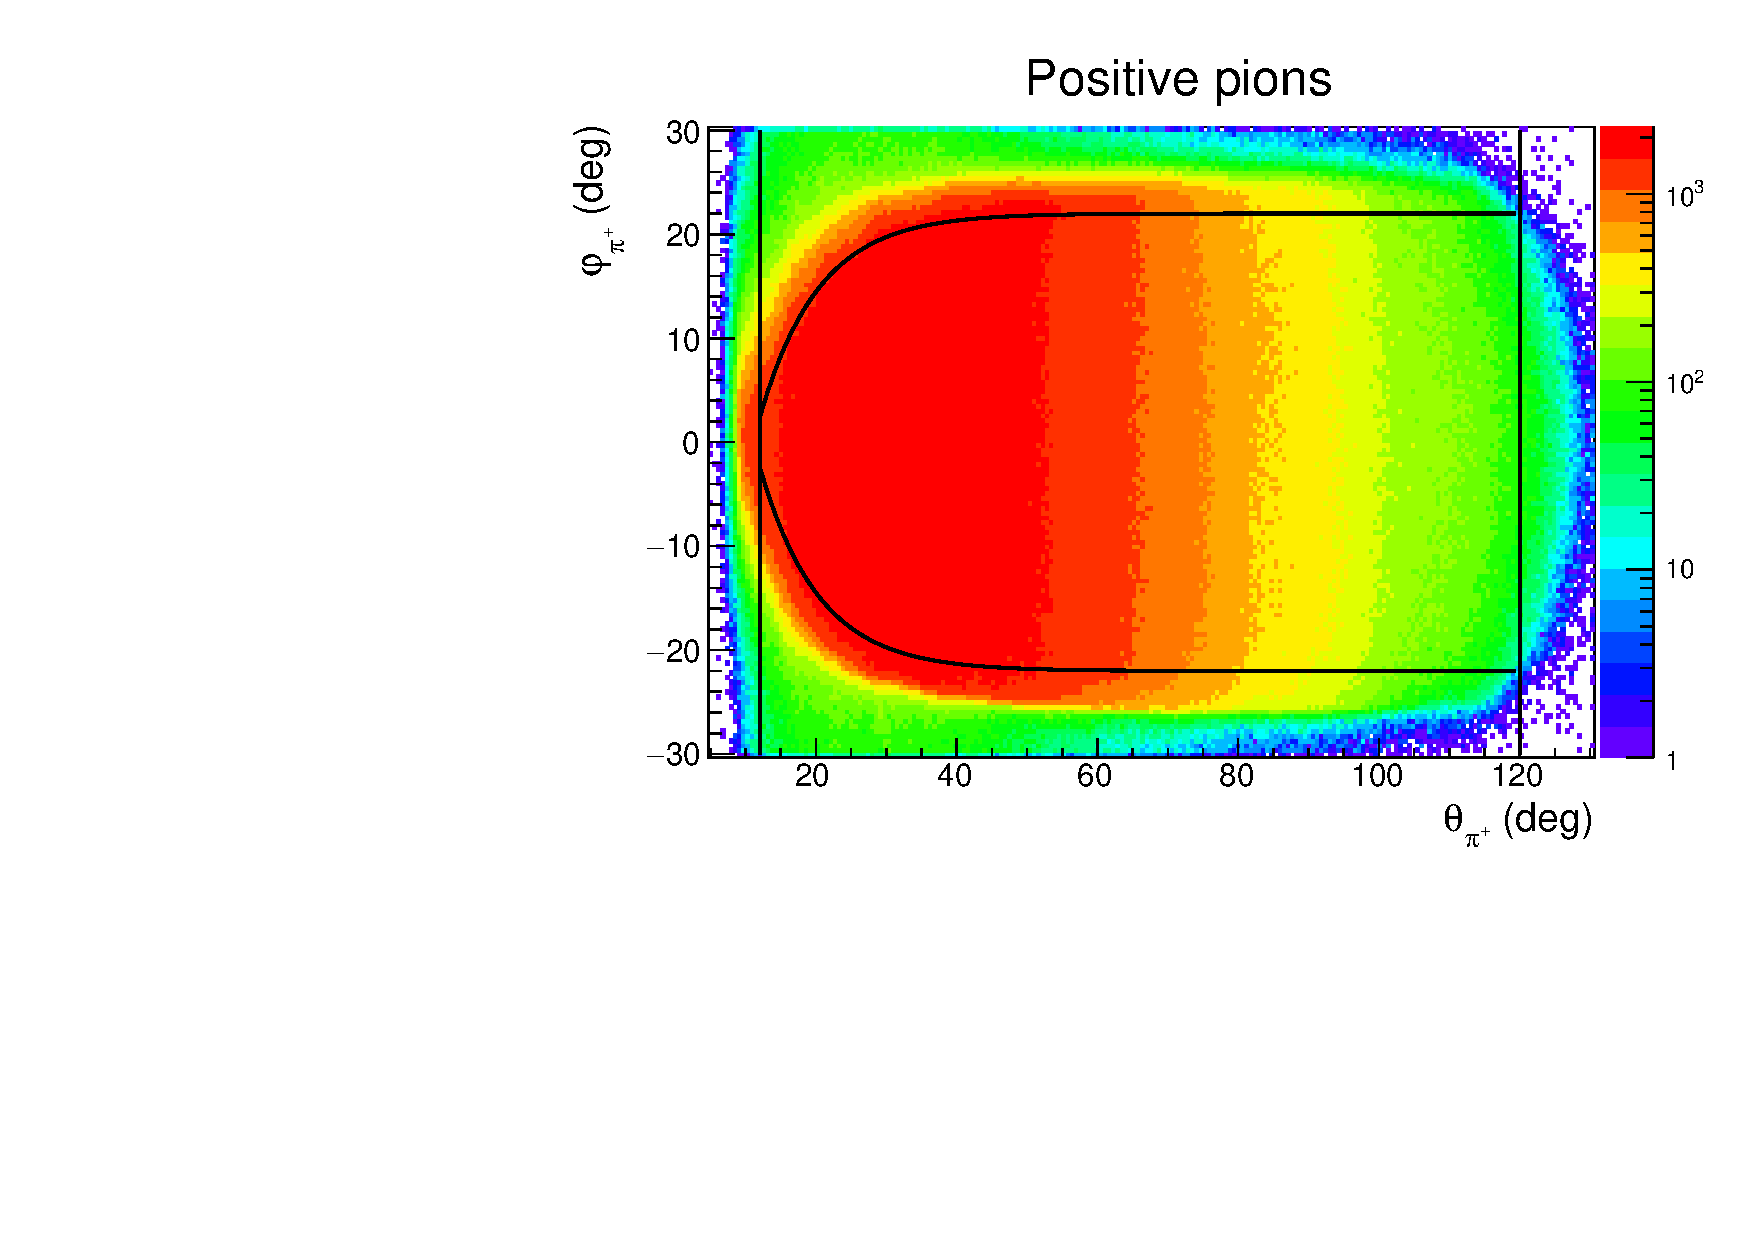
\includegraphics[width=0.4\textwidth]{pictures/other_cuts/fiducial/fid_pip_2dim.pdf}}
\end{center}
\caption{\small $\varphi$ versus $\theta$ distributions for positive hadron candidates: left plot -- for protons, right plot -- for positive pions. The distributions are plotted for events from all CLAS sectors. Curves show the applied fiducial cuts given by Eq.~\eqref{eq:fiduch_pos}, vertical lines stand for $\theta^{min}$ and $\theta^{max}$. The angles are taken at the interaction vertex.}
\label{fig:fiduch_pos_2d}
\end{figure}

Additional fiducial cuts in $\theta$ versus momentum coordinates are shown by the black curves for the data and reconstructed Monte Carlo events in Fig.~\ref{fig:th_vs_p_pr} for protons and in Fig.~\ref{fig:th_vs_p_pip} for $\pi^{+}$.


\clearpage

\begin{figure}[htp]
\begin{center}
\framebox{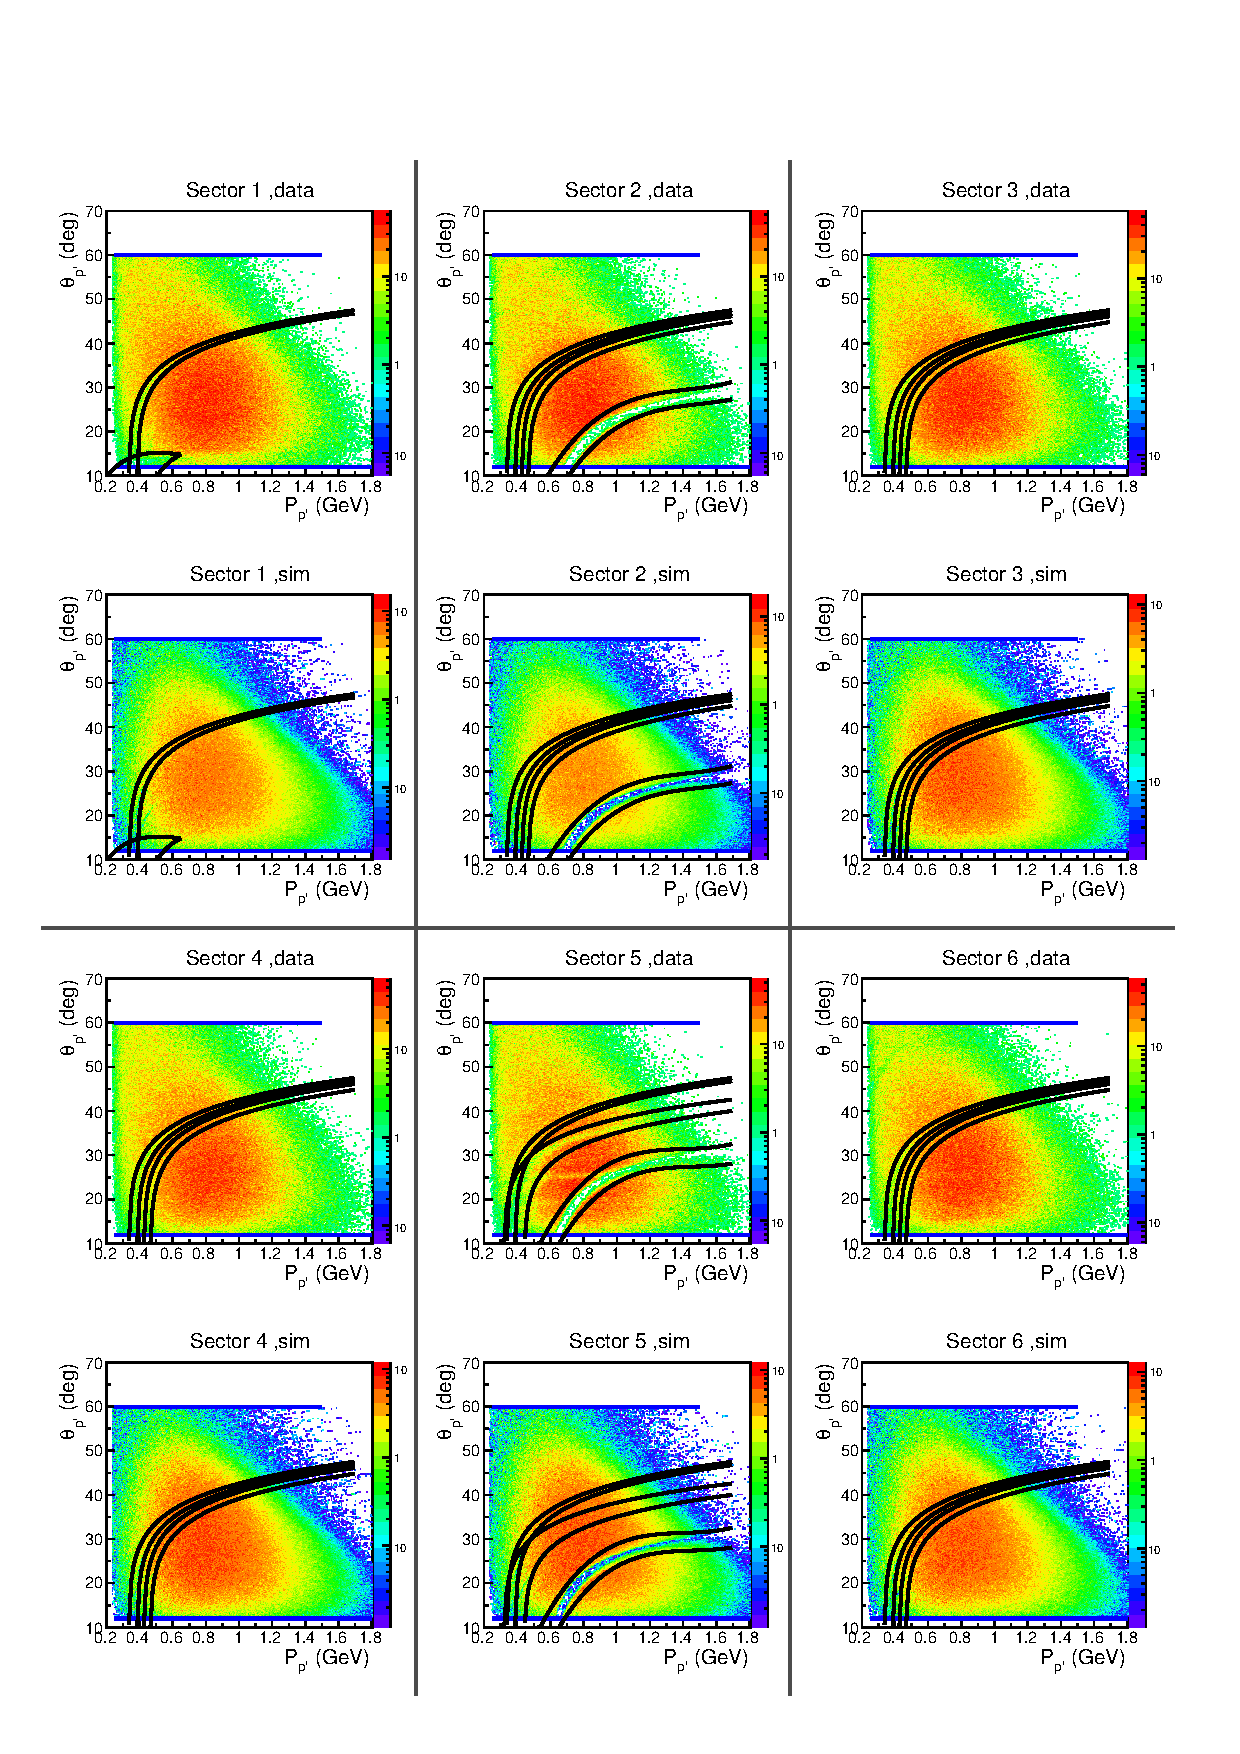
\includegraphics[width=14.5cm]{pictures/other_cuts/fiducial/th_vs_p_pr.pdf}}
\caption{\small $\theta$ versus momentum distributions for proton candidates for different CLAS sectors. The angle $\theta$ is taken at the interaction vertex. Plots are given both for the real data and reconstructed Monte Carlo events. Blue lines correspond to $\theta^{min}$ and $\theta^{max}$ in Eq.~\eqref{eq:fiduch_pos}. Black curves correspond to additional fiducial $\theta$ versus momentum cuts. \label{fig:th_vs_p_pr}}
\end{center}
\end{figure}

\clearpage

\begin{figure}[htp]
\begin{center}
\framebox{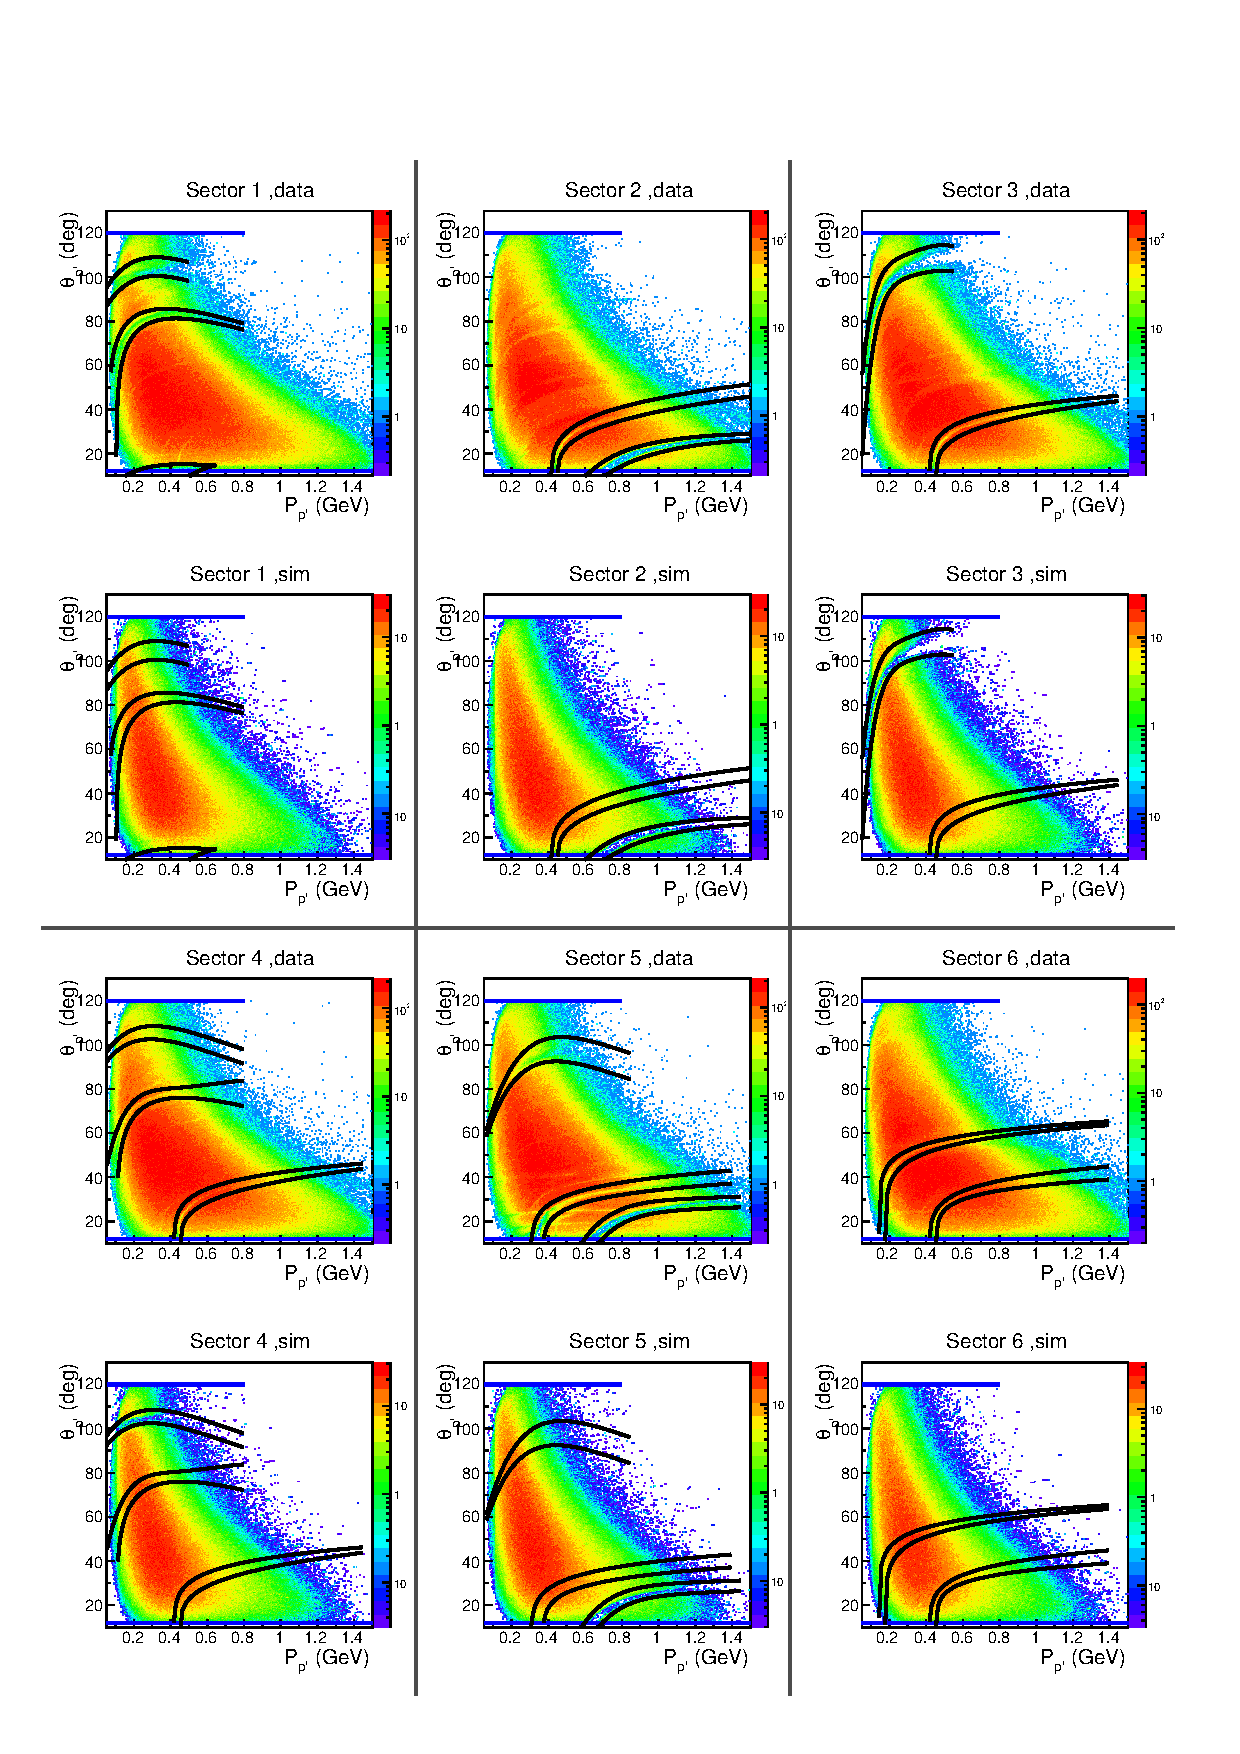
\includegraphics[width=14.5cm]{pictures/other_cuts/fiducial/th_vs_p_pip.pdf}}
\caption{\small $\theta$ versus momentum distributions for positive pion candidates for different CLAS sectors. The angle $\theta$ is taken at the interaction vertex. Plots are given both for the real data and reconstructed Monte Carlo events. Blue lines correspond to $\theta^{min}$ and $\theta^{max}$ in Eq.~\eqref{eq:fiduch_pos}. Black curves correspond to additional fiducial $\theta$ versus momentum cuts. \label{fig:th_vs_p_pip}}
\end{center}
\end{figure}

\clearpage

\subsection{Data quality check}
\label{Sect:qcheck}
\afterpage{\clearpage}

During a long experimental run, variations of the experimental conditions, e.g. fluctuations in the target density, deviations of the beam current and position as well as changes in the response of parts of the detector, can lead to fluctuations in event yields. Only the parts of the run with relatively stable event rates are selected for the analysis.
Therefore, cuts on Data Acquisition (DAQ) live time and number of events per Faraday cup (FC) charge need to be established.
%\footnote[1]{This quality check cuts are used only for the full target runs}. 

\afterpage{\clearpage}
\begin{figure}[htp]
\begin{center}
\framebox{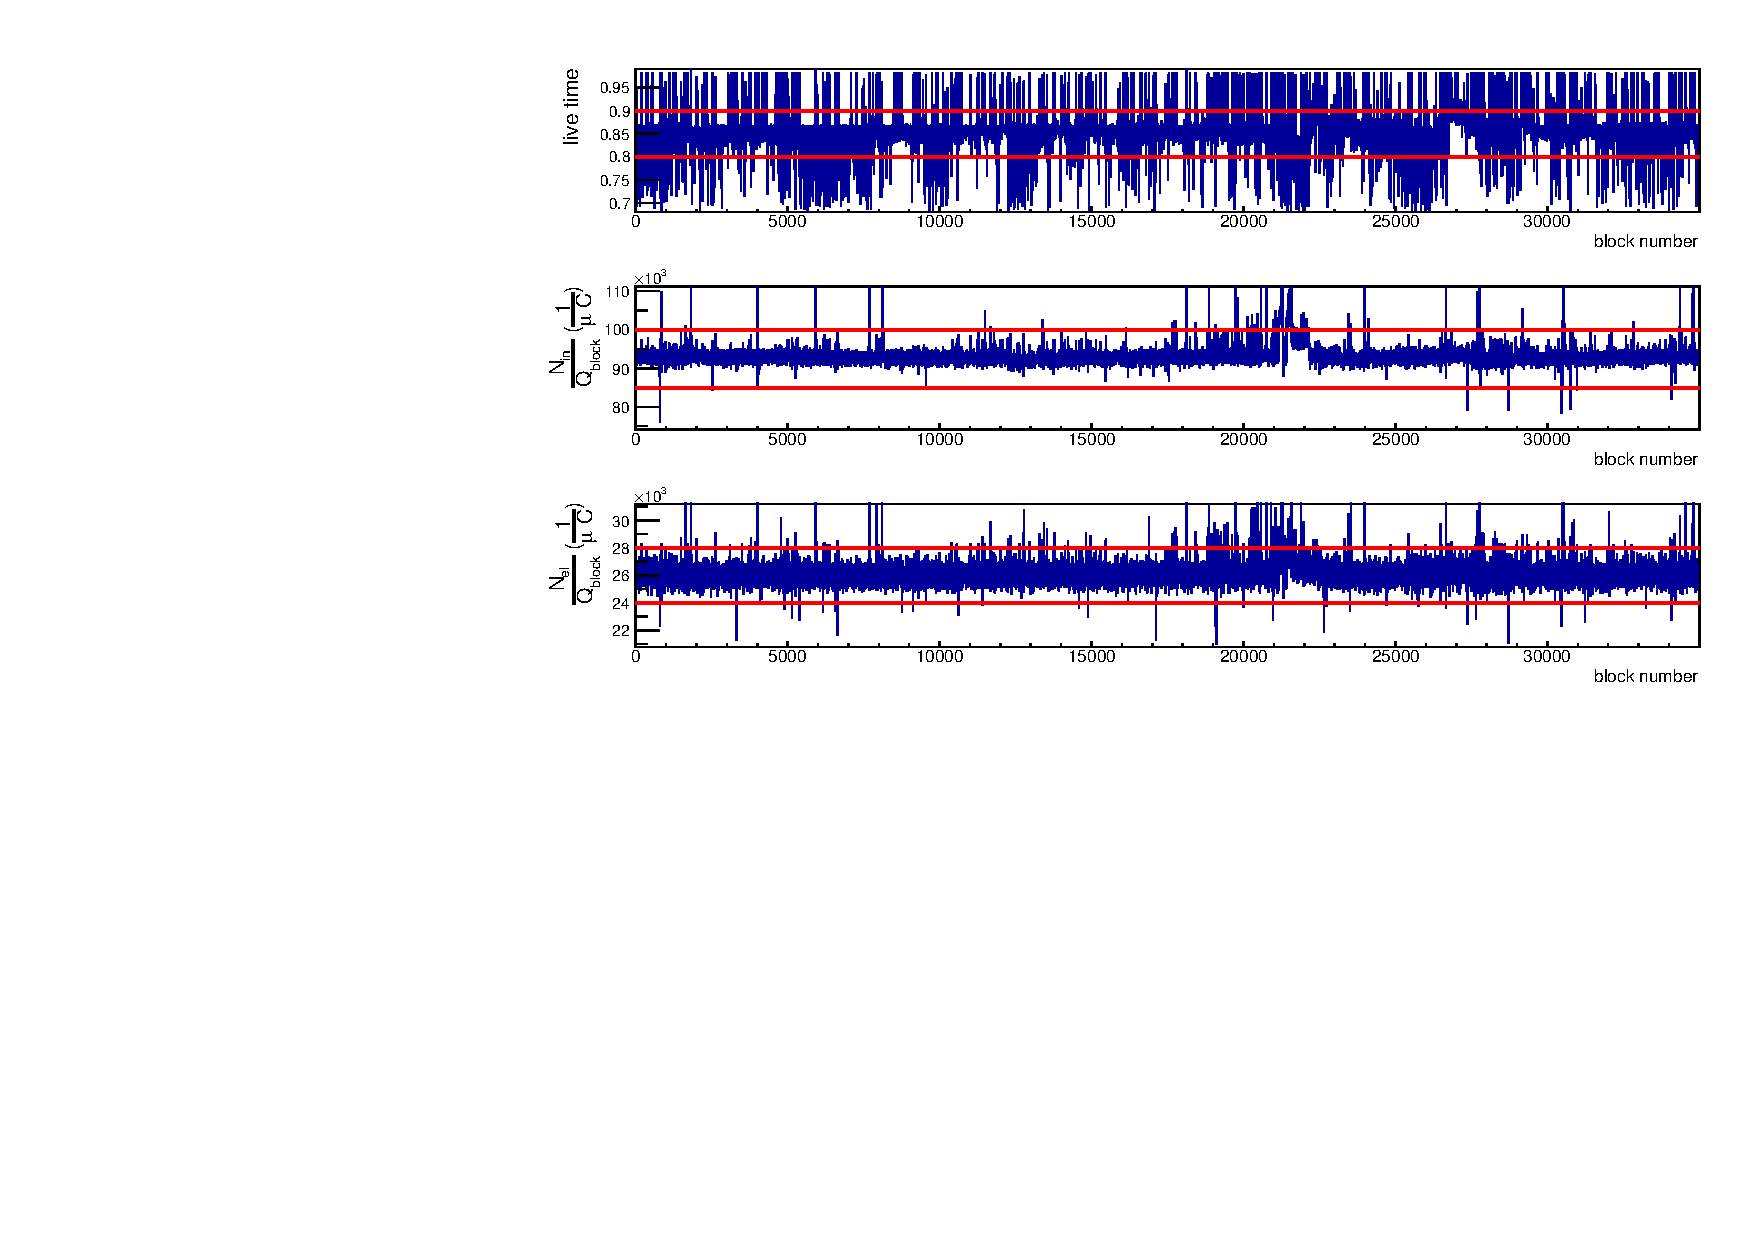
\includegraphics[width=\textwidth]{pictures/other_cuts/qual_check/livetime_incl_elast_2d_norebin.pdf}}
\caption{\small In the top plot DAQ live time is shown as a function of {\em block} number. Each {\em block} corresponds to  the portion of events that is accumulated during a single Faraday cup charge reading cycle. {\em Block} numbers range from one to the maximum number and represent the run duration in the units of Faraday cup readouts. In the middle plot the number of inclusive events accumulated within each {\em block} divided by FC charge accumulated during the {\em block} is  plotted versus {\em block} number. The bottom plot shows the number of elastic events accumulated within each {\em block} divided by FC charge accumulated during the {\em block} as a function of {\em block} number. Horizontal red lines show the applied cuts.  \label{fig:qual_check_2d}}
\end{center}
\end{figure}\vspace{-0.75em}

The FC charge updates with a given frequency, so the whole run time can be divided into so-called {\em blocks}. Each {\em block} corresponds to the portion of time between two FC charge readouts. FC charge readouts happen approximately once every ten seconds. The {\em block} number ranges over the run time from one to a certain maximum number. The first and last {\em blocks} in each run file are excluded from the analysis, since FC readout is not synchronized in time with the start/stop of writing to the file.


The DAQ live time is the portion of time within the {\em block} during which the DAQ system is able to accumulate events. A significant deviation of the live time from the average value indicates event rate alteration. For instance, if the live time is close to one, then the event rate is too low and vice versa.
In Fig.~\ref{fig:qual_check_2d} the DAQ live time (top plot) as well as the yields of inclusive (middle plot) and elastic (bottom plot) events normalized to FC charge are shown as a function of {\em block} number. {\em Blocks} between the horizontal red lines in Fig.~\ref{fig:qual_check_2d} are selected for the analysis.
Due to the enormous amount of {\em blocks} all of them cannot be made visible in two-dimensional histograms, therefore, to have a general feeling of what amount of blocks are removed, the $y$-axis projections of the histograms in Fig.~\ref{fig:qual_check_2d} are given in Fig.~\ref{fig:qual_check_1d}. The horizontal red cut lines in Fig.~\ref{fig:qual_check_2d} correspond to the vertical red cut lines in Fig.~\ref{fig:qual_check_1d}.

\afterpage{\clearpage}
\begin{figure}[htp]
\begin{center}
\framebox{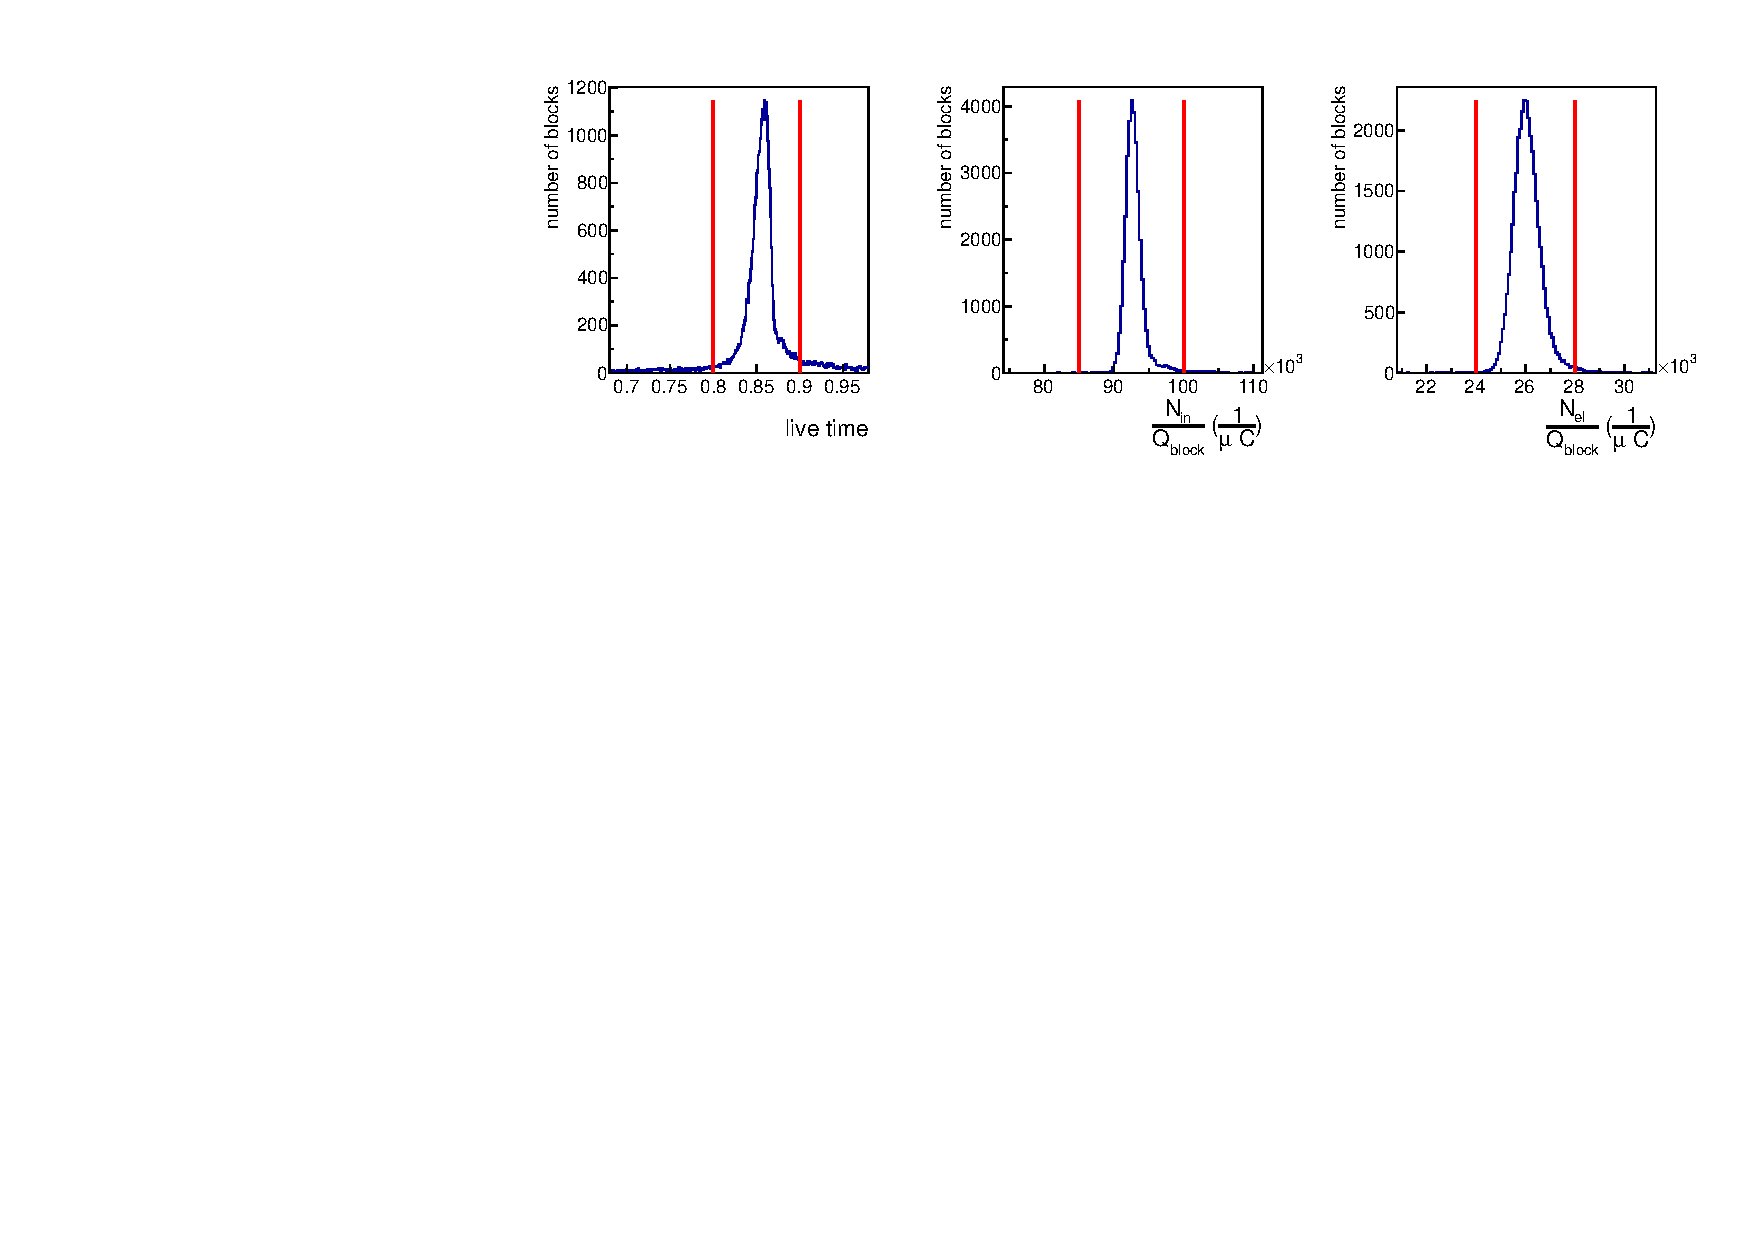
\includegraphics[width=\textwidth]{pictures/other_cuts/qual_check/livetime_incl_elast_1d.pdf}}
\caption{\small Number of {\em block} occurrences (see explanation in the text) as a function of DAQ live time (left plot), inclusive event yield normalized to FC charge  (middle plot), and  elastic event yield normalized to FC charge (right plot). The vertical red cut lines correspond to the horizontal red cut lines in Fig.~\ref{fig:qual_check_2d}. \label{fig:qual_check_1d}}
\end{center}
\end{figure}



\subsection{Vertex cut}
\label{Sect:vertex}
\afterpage{\clearpage}

The ``e1e" experiment employed a specific target~\cite{target} with the same assembly for the hydrogen and the deuterium parts of the run period. The target setup is presented in Fig.~\ref{fig:e1e_target}. The conical shape of the target (with the diameter varying from 0.35 to 0.6 cm) serves the purpose of effective extraction of gas bubbles, which are formed in the liquid target content due to the heat that either originates from the beam and/or comes from outside through the target walls. Due to the conical shape, the bubbles are drained upwards and into a wider area of the target thus clearing the beam interaction region and allowing the boiled deuterium to be effectively delivered back to the cooling system to be condensed. 

The target cell had 15-$\mu$m-thick aluminum entrance and exit windows. In addition, an aluminum foil was located 2.0 cm downstream of the target. This foil was made exactly the same as the entry/exit windows of the target cell and served for both the estimation of the number of events that originated in the target windows and the precise determination of the target $z$-position along the beamline.

\begin{figure}[!ht]
\begin{center}
\framebox{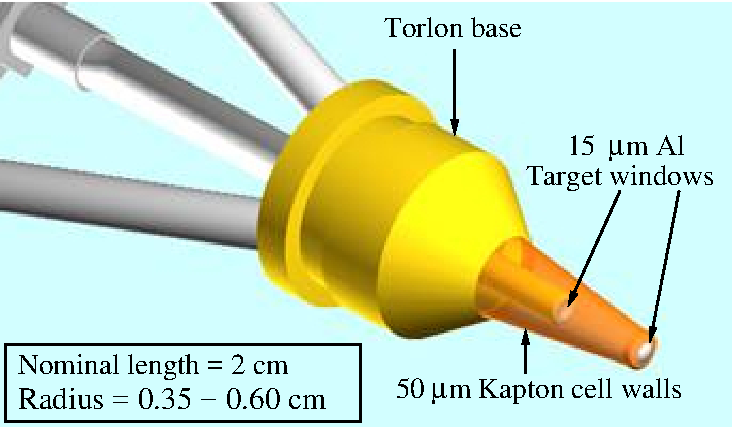
\includegraphics[width=10cm]{pictures/other_cuts/z_vertex/e1e_target_small.pdf}}
\end{center}
\caption{\small LH$_{2}$/LD$_{2}$ target cell and its support structure used during ``e1e" run period~\cite{target}.  }
\label{fig:e1e_target}
\end{figure}


In Fig.~\ref{fig:z_el_full_empty} distributions of electron $z$-coordinate at the interaction vertex are shown for events from both empty and full target runs for all six CLAS sectors. The vertical red lines show the cut that is applied in addition to the empty target event subtraction. The vertical dashed line marks the position $z = -0.4$~cm, where the center of the target is expected to be. However, as seen in Fig.~\ref{fig:z_el_full_empty}, the $z_{e'}$ distributions demonstrate small sector dependent deviations from their expected position. The source of these deviations is an offset of the beam position from the CLAS central line $(x, y) = (0, 0)$. 

To estimate the beam offset, the $y_{e'}^{dc}$ versus $x_{e'}^{dc}$ distribution was investigated, where $x_{e'}^{dc}$ and $y_{e'}^{dc}$ are the corresponding coordinates of an electron at the point of interaction, which are taken from the DCPB bank (variables $\rm X\_v$ and $\rm Y\_v$, respectively). This distribution is shown in Fig.~\ref{fig:beam_offset}, where the intersections of black dashed and solid red lines indicate the nominal and actual beam positions, respectively. The actual beam position was found to be ($x$,~$y$) = (0.057~cm,~-0.182~cm). The generated Monte Carlo events were reconstructed taking into account the determined beam offset to improve resemblance to the real data\footnote[7]{The following option was used in the {\em ffread card}: POSBEAM 0.057 -0.182.}.

In Fig.~\ref{fig:z_el_data_sim} event distributions after the subtraction of the empty target contribution are shown in comparison with Monte Carlo events reconstructed taking into account the beam offset. As can be seen in this figure the simulation matches the data well enough and almost completely reproduces the sector dependent deviation of the distributions from the nominal position marked by the black dashed lines.

\afterpage{\clearpage}
\begin{figure}[!ht]
\begin{center}
\framebox{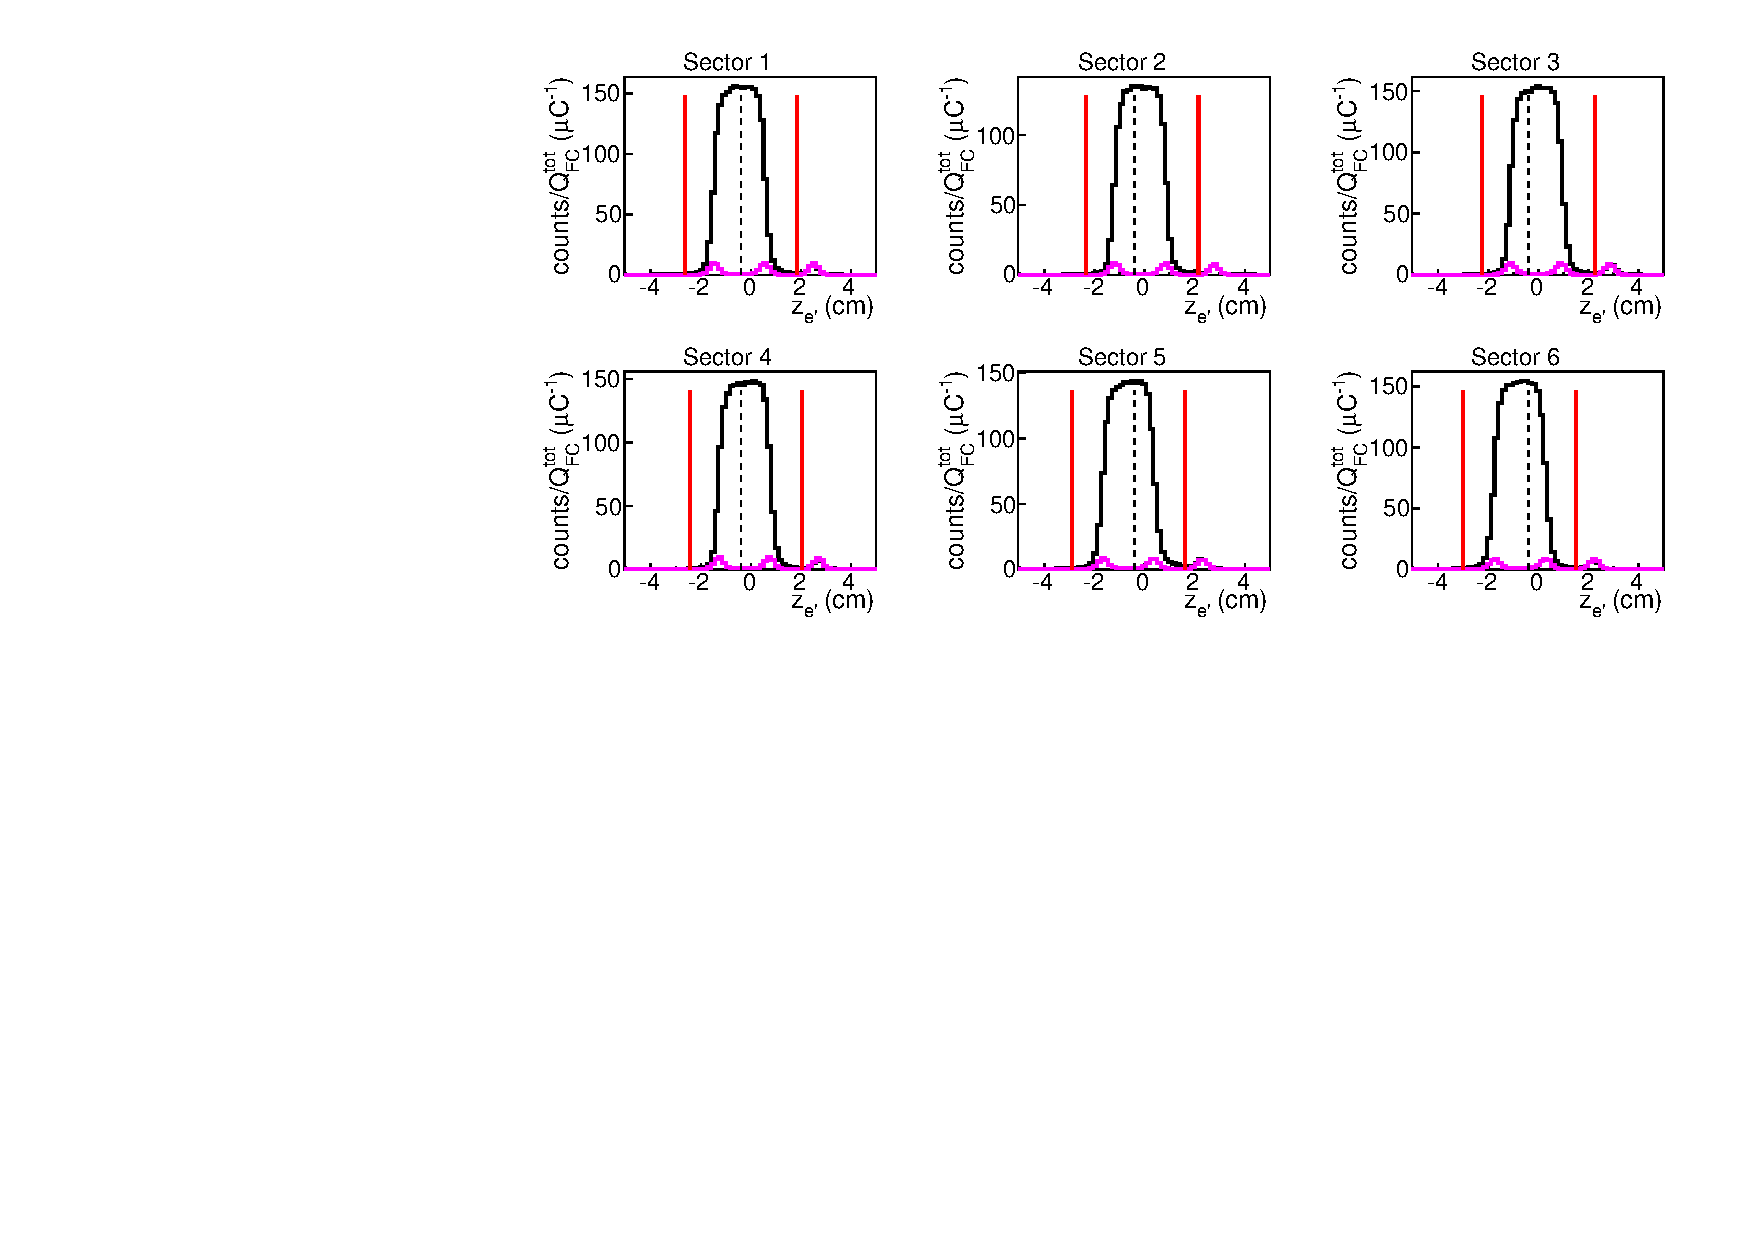
\includegraphics[width=13.1cm]{pictures/other_cuts/z_vertex/z_el_full_empty3.pdf}}
\end{center}
\caption{\small Distributions of the electron $z$-coordinate at the vertex for full (black curves) and empty (magenta curves) target runs for the six CLAS sectors. Vertical dashed lines mark the position $z = -0.4$~cm, where the center of the target is expected to be. Vertical red lines show the applied cuts. Both full and empty target distributions are normalized to the corresponding FC charge. }
\label{fig:z_el_full_empty}
\end{figure}

\begin{figure}[!ht]
\begin{center}
\framebox{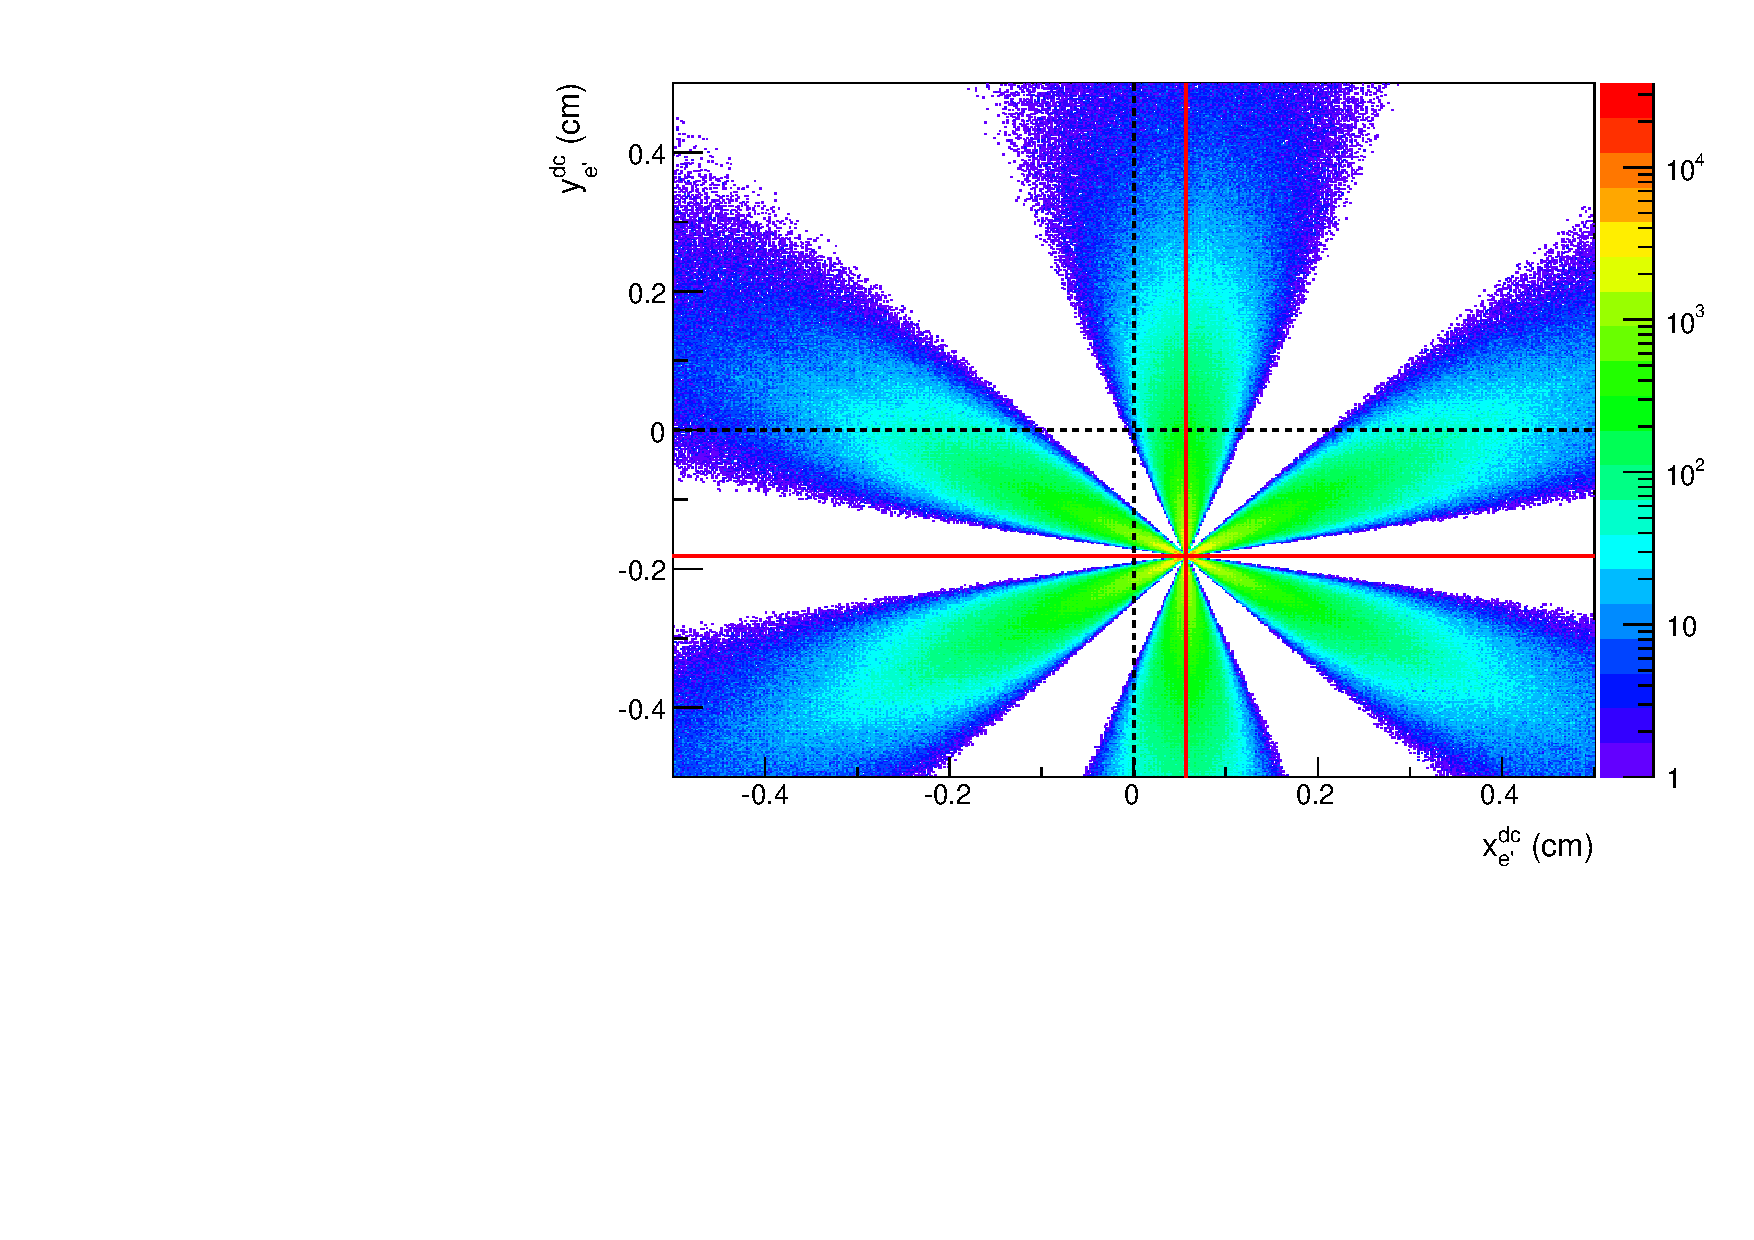
\includegraphics[width=11cm]{pictures/other_cuts/z_vertex/beam_offset.pdf}}
\end{center}
\caption{\small $y_{e'}^{dc}$ versus $x_{e'}^{dc}$ distribution that demonstrates the beam offset. Black dashed lines mark the position ($x$,~$y$) = (0,~0), where the beam is expected to be. Red lines demonstrate the actual beam position at ($x$,~$y$) = (0.057~cm,~-0.182~cm). }
\label{fig:beam_offset}
\end{figure}



\begin{figure}[!ht]
\begin{center}
\framebox{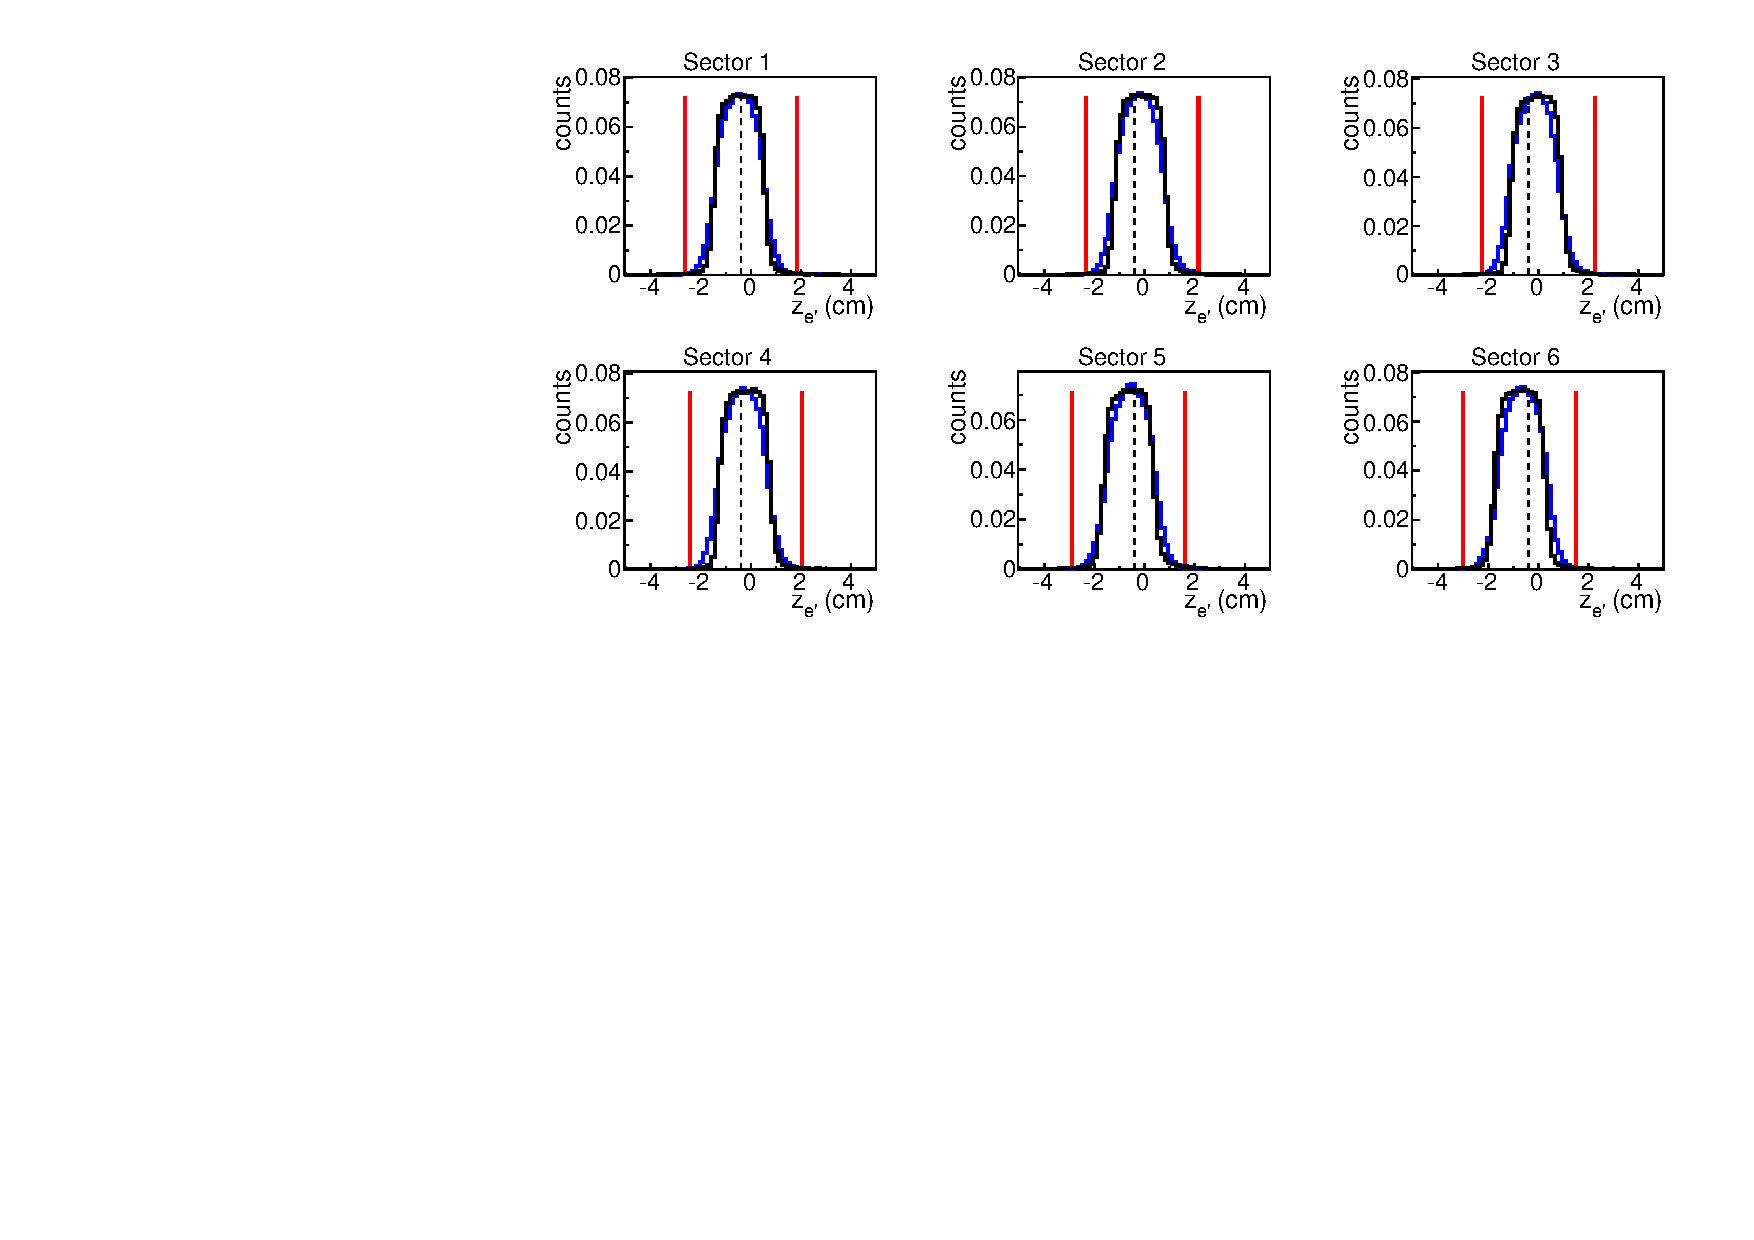
\includegraphics[width=13.1cm]{pictures/other_cuts/z_vertex/z_el_data_sim3.pdf}}
\end{center}
\caption{\small Distributions of the electron $z$-coordinate at the vertex for the experimental data (black curves) and the Monte Carlo events reconstructed taking into account the beam offset (blue curves) for the six CLAS sectors. For the data empty target contributions are subtracted. Vertical dashed lines mark the position $z = -0.4$~cm, where the center of the target is expected to be. Vertical red lines show the applied cuts. All distributions are normalized to the integral. }
\label{fig:z_el_data_sim}
\end{figure}

\begin{figure}[!ht]
\begin{center}
\framebox{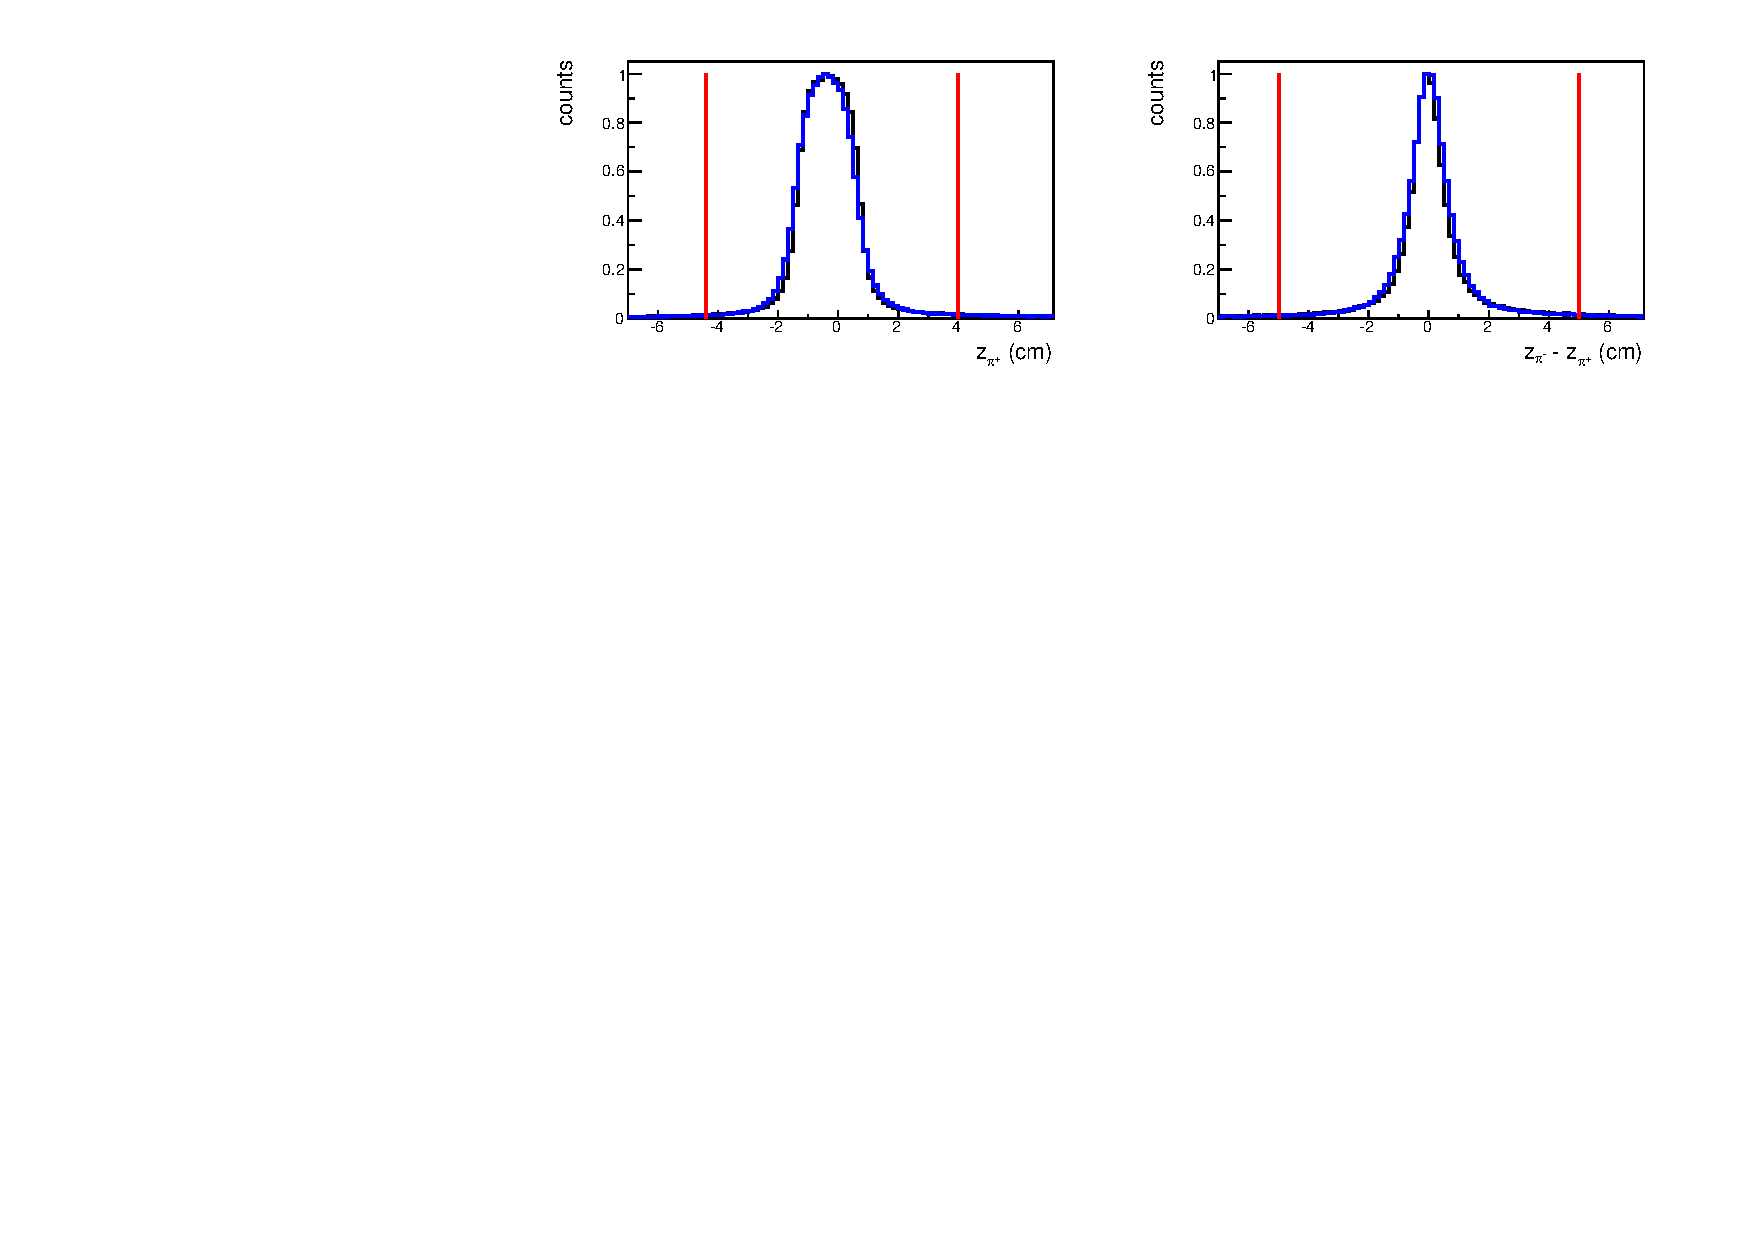
\includegraphics[width=13.1cm]{pictures/other_cuts/z_vertex/additional_cuts.pdf}}
\end{center}
\caption{\small Left plot: an example of the cut on the hadron $z$-coordinate, $|z_{\pi^{+}} + 0.4| < 4.4$~cm. Right plot: an example of the cut on the difference of the vertex $z$-coordinates of the final particles, $|z_{\pi^{-}} - z_{\pi^{+}}| < 5$~cm. The black curves correspond to the data, while the blue ones correspond to the reconstructed Monte Carlo events. All histograms are normalized to their maxima.}
\label{fig:add_cuts_vert}
\end{figure}
\newpage
To reduce the number of events in which the final state particles came from different events and/or took part in final state interactions, the following two additional cuts on the particle $z$-coordinates at the vertex are applied. The first cut is $|z_{h} + 0.4| < 4.4$~cm, where the index $h$ corresponds to the final hadron type (proton, $\pi^{+}$, and $\pi^{-}$). The left side of Fig.~\ref{fig:add_cuts_vert} shows an example of this cut for the case $h=\pi^{+}$. The second cut is $|z_{i} - z_{j}| < 5$~cm, where the indices $i$ and $j$ ($i\neq j$) correspond to the final particle type (electron, proton, $\pi^{+}$, and $\pi^{-}$). The right side of Fig.~\ref{fig:add_cuts_vert} shows an example of this cut for the case $i=\pi^{-},~j=\pi^{+}$. These additional cuts are made rather loose in order to avoid unjustified loss of good events.


%\subsection{A few more minor cuts}

%\begin{itemize}
%\item missing energy cuts,
%\item invariant masses border cuts,
%\item cuts on the number of particles.


%\end{itemize}

\newpage
\section{Exclusivity cut in the presence of Fermi smearing and FSI}
\label{Sect:excl_cut}

For picking out certain exclusive reactions one needs to register the scattered electron and either all final hadrons or all except one. In the latter case the four-momentum of the unregistered hadron can be restored using energy-momentum conservation (a so-called ``missing mass technique"). Thus for the reaction $e p \rightarrow e' p' \pi^{+} \pi^{-} $ one can in general distinguish between four so-called ``topologies" depending on the specific combination of registered final hadrons. In this particular analysis the following two topologies are analyzed,%\vspace{-0.25em}
\begin{itemize}
\item the fully exclusive topology (all final particles are registered) $e p \rightarrow e' p' \pi^{+} \pi^{-} X$, and%\vspace{-0.25em}
\item the $\pi^{-}$ missing topology $e p \rightarrow e' p' \pi^{+} X$.
\end{itemize} %\vspace{-0.25em}


Due to the experimental conditions the statistics of the fully exclusive topology is very limited. This happens mainly because CLAS does not cover the polar angle range $0\,^{\circ}\mathrm{} < \theta_{lab} < 8\,^{\circ}\mathrm{}$~\cite{Mecking:2003zu}. The presence of this forward acceptance
hole does not affect much the registration of the positive particles ($p$ and $\pi^{+}$), since their trajectories are bent by the magnetic field away from the hole. Meanwhile, the negative particles ($e$ and $\pi^{-}$) are inbending, which means that their trajectories are bent into the forward direction. Electrons being very light and rapid undergo small track curvature, and the presence of the forward hole leads for them only to a constraint on the minimum achievable $Q^2$. However, for negative pions the situation is dramatic: being heavier and slower they are bent dominantly into the forward detector hole and, therefore, most of them cannot be registered. This leads to the fact that the $\pi^{-}$ missing topology contains the dominant part of the statistics. The contribution of the fully exclusive topology to the total analyzed statistics\footnote[8]{The combined statistics of both the $\pi^{-}$ missing and the fully exclusive topologies.} varies from $\sim$5\% near the reaction threshold to $\sim$25\% at $W\sim 1.7-1.8$~GeV. 
 
For reactions with multi-particle final states the problem of limited acceptance is an essential issue. Specifically, in the case of the $p\pi^{+}\pi^{-}$ final state the cross section  depends on five final hadron variables and hence is multi-dimensional, but the limited statistics only allows the extraction of a set of one-fold differential cross sections (see Sects.~\ref{Sect:kin_var} and ~\ref{Sect:cr_sect_formula}). This leads to the necessity to fill kinematic cells with zero acceptance (so-called ``empty cells") based on some model assumptions, which leads to model dependent results (see Sect.~\ref{Sect:empt_cells}). The fully exclusive topology suffers from the problem of limited acceptance (and therefore large amount of empty cells) that along with the problem of limited statistics does not allow any sensible cross section information to be obtained from this topology alone. The $\pi^{-}$ missing topology, having significantly fewer empty cells, serves the purpose of the cross section extraction best. The use of both topologies combined allows the model dependence of the cross section (that originates from empty cells filling) to be reduced as well as slightly increasing the statistics.

The aforementioned features of the two topologies are caused by the experimental conditions and valid either for an experiment off the free proton or for one off the proton bound in the deuteron. Meanwhile, there are also some features that appear only in bound proton experiments. Those that are crucial for exclusive event selection are addressed later in this Section, while others are discussed later in the report.

Actually, two more topologies can be distinguished, i.e. the proton missing topology and the $\pi^{+}$ missing topology. Both require registration of the $\pi^{-}$ in the final state and as a consequence suffer from the similar problems of suppressed statistics\footnote[9]{Each of them contains about 10\% of the full statistics of all four topologies combined.} and limited acceptance as in the case of the fully exclusive topology.  Therefore, these two topologies are usually ignored in analyses of the reaction $ep\rightarrow{}e'p'\pi^{+}\pi^{-}$~\cite{Rip_an_note:2002,Ripani:2002ss,Fed_an_note:2007,Fedotov:2008aa,Isupov:2017lnd}. Nevertheless, as demonstrated in the sophisticated analysis of this reaction off the free proton target~\cite{Fed_an_note:2017,Fed_paper_2018}, they can be used as complimentary topologies to the main $\pi^{-}$ missing topology, that allows a slight increase in the statistics and a reduction in the amount of empty cells as much as possible, therefore minimizing the model dependence of the extracted cross sections. However, if the pion pair is produced off the proton bound in the deuteron, additional complications appear: these topologies turn out to be polluted with events from other reaction channels. In the proton missing topology the missing mass technique fails to distinguish whether the pion pair was produced off the proton or off the neutron, because their masses are almost identical. A similar situation occurs for the $\pi^+$ missing topology, where the same reason prevents distinguishing between the production of $\pi^{+}\pi^{-}$ pair off the proton and $\pi^{0}\pi^{-}$ pair off the neutron, if only the proton and the $\pi^{-}$ in the final state are registered. Moreover, the event sample in the $\pi^+$ missing topology demonstrates strong admixture of events from the reaction $en(p)\rightarrow e'p'(p')\pi^{-}$, which was found to be not very easy to remove.
 
Taking into account all the above arguments, the following topology ranking takes place in this particular analysis: the $\pi^{-}$ topology is the main one and the fully exclusive topology is treated as the complimentary one, which gives a slight increase in statistics as well as some reduction in the amount of empty cells, while the proton missing and the $\pi^{+}$ missing topologies are not used at all.

Meanwhile, an experiment on bound nucleons has some specific features, which are extrinsic to the free proton experiments. Those of them that are related to the problem of the channel identification are listed below.%\vspace{-0.25em}

\begin{itemize}
\item  The Fermi motion of the target proton.% \vspace{-0.25em}
\item Complex effects of Final State Interactions (FSI) due to the presence of the neutron and the multi-particle final state.
\end{itemize}%\vspace{-0.25em}

The manifestations of these effects in the $\pi^{-}$ missing and fully exclusive topologies differ.

The movement that the target proton undergoes in the deuterium nucleus is concealed from the observer and is not measured\footnote[10]{In general it can be measured by detecting the recoil nucleon (neutron in this case), but it was not an option in this experiment.}. However, if all particles in the final state are registered, one can restore the information about the momentum distribution of the target proton via energy-momentum conservation (see Sect.~\ref{Sect:excl_cut_fully_excl} for details). This is not the case for the $\pi^{-}$ missing topology, where incomplete knowledge about the final state leads to the fact that information about the motion of the initial proton turns out to be totally lost. Therefore, one is forced to work under a so-called ``target-at-rest-assumption" that considers the target proton to have no motion and as a consequence inevitably leads to the smearing of various kinematic quantities, such as missing mass, reaction invariant mass ($W$), etc~\cite{Skorodumina:2015rea}. 
Although the fully exclusive topology has the advantage of the possibility of avoiding the smearing\footnote[11]{For example, in the fully exclusive topology the value of $W$, being calculated using the four-momenta of the registered final hadrons, turns out to be determined within the detector resolution and not affected by the effects of the target motion.}, all kinematic quantities are nevertheless calculated under the target-at-rest-assumption in order to treat this complimentary topology in the same way as the main one.


In order to reliably identify the exclusive channel and correctly calculate the detector efficiency, the distributions of the reconstructed Monte Carlo events must match experimental ones as well as possible. As mentioned above, the necessity to work under the target-at-rest-assumption smears the experimental distributions, which in turn demands the simulated distributions reproduce this smearing. Therefore, the effects of the target motion must be properly included in the Monte Carlo simulation.

That is why the event generator TWOPEG-D~\cite{twopeg-d} was used to perform the Monte Carlo simulation. It is a version of the TWOPEG (event generator for double-pion electroproduction off the free proton~\cite{twopeg}) that was developed for this analysis in order to simulate the effects of the target motion. In this version of the event generator the Fermi motion of the initial proton is generated according to Bonn potential~\cite{Machleidt:1987hj} and then naturally merged into the specific kinematics of double-pion electroproduction.

The second intrinsic feature of a bound nucleon experiment is the complex effects of FSI. This phenomenon is driven by the strong interaction and consists in the fact that after the production of the final state hadrons and before their registration they manage to interact with each other and/or the recoil nucleon. These interactions include (but are not limited to) the simple momentum exchange between the hadrons as well as the process of exciting nucleon resonances with their subsequent decay that may lead to the production of new particles. 


Final hadrons produced off the free proton are also subject to the FSI, but in the absence of the recoil neutron these interactions are not substantial. The arguments for that are the following. The probability to interact in the final state depends on the distance between hadrons and their relative velocity, i.e. for slower and closer travelling hadrons the chance to interact is higher then for distant and rapid hadrons. Final state hadrons are produced in one vertex, which means that in the beginning they are very close to each other and therefore have a high chance to interact. However, immediately after the production they start to fly apart from the vertex in radial directions increasing the distance between each other, which causes the interaction probability drop.



The presence of an additional recoil nucleon changes the situation drastically. The neutron, which initially was not involved into the reaction of hadron production, is located slightly aside of the interaction vertex but at the same time very close to it, so that the flying-off final hadrons can impact the neutron. In addition to that, the neutron also moves with Fermi momentum, thus the FSI are brought to the usual hadron-hadron collisions, which may result in the resonance excitation and/or particle production. Direct hadron-hadron collisions, which are unlikely to occur in the reaction off the free proton, since the final hadrons fly apart from one point, start to play a role in the reaction off the bound proton in the presence of the neutron. Therefore, FSI effects in the bound nucleon experiment are rather strong in contrast to those in the free proton one.

\begin{figure}[!ht]
\begin{center}
\framebox{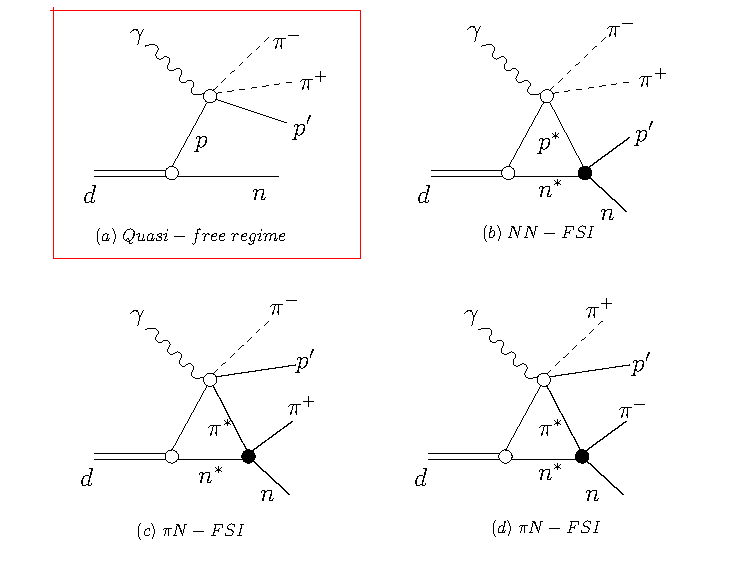
\includegraphics[width=13cm]{pictures/other_cuts/excl_cut/fsi_mech.pdf}}
\end{center}
\caption{\small Illustration of the leading contributors to the process of the double-pion production off the proton bound in deuteron. (a) Quasi-free regime, (b) NN-FSI, and (c-d) $\pi N$-FSI.}
\label{fig:fsi_mech}
\end{figure}

FSI affect the final hadron momenta, making them either distorted by rescattering effects or leak away via the production of extra particles in hadron-hadron collisions. This leads to the distortion of various kinematic quantities, such as missing masses. If the final hadrons manage to avoid any interaction with the neutron, then the neutron is treated as a spectator and the reaction is considered to occur in a so-called ``quasi-free regime". Figure~\ref{fig:fsi_mech} schematically illustrates the production of the pion pair off the bound proton in the quasi-free regime (a) as well as the leading components for FSI of the final hadrons with the neutron (b-d), which result in so-called ``FSI-disturbed kinematics". The goal of this study is to extract the cross sections of the process (a), which implies the need to select for the analysis only events in quasi-free kinematics. This in turn means removing from consideration those events in which final hadrons have undergone FSI.



In contrast to the effects of the target motion, which can be simulated fairly easy, the effects of FSI can hardly be taken into account in the simulation because they are of very complex nature and hence not yet fully understood. Therefore, the Monte Carlo simulation is not able to reproduce the distortions due to FSI that occur in some experimental distributions, but this is not a problem if events in quasi-free kinematics are properly separated from those in FSI-disturbed kinematics. This leads to the necessity to develop special procedures of selecting quasi-free events as well as correcting for the remaining admixture of undesired events, if they cannot be fully eliminated.

The yield of events in FSI-disturbed kinematics turned out to strongly depend on (i) the reaction invariant mass ($W$) and (ii) on the hadron scattering angles. The latter issue causes FSI effects to manifest themselves differently depending on the reaction topology, since the topologies have non-identical geometrical acceptance.%, that in turns forces us to select quasi-free event in each topology individually. 

As follows from the above, the two analyzed topologies differ from each other both in treating of the Fermi motion of the initial proton and in FSI manifestations. Therefore, the channel identification in the quasi-free regime was performed in each topology individually (see subsequent subsections). 


The problem of background channels is also an issue that deserves special attention for the bound proton experiment. For the reaction of double-pion production off the free proton the main background channel is $ep\rightarrow e'p'\pi^{+}\pi^{-}\pi^{0}$. In the analysis~\cite{Fed_an_note:2017} that was carried out for the same beam energy $E_{beam} = 2.039$~GeV, it is shown that although the admixture of the events from this background channel becomes discernible at $W\gtrsim 1.6$~GeV, it remains negligible and well separated from the double-pion events via the exclusivity cuts. For the experiments with the deuteron target the reaction $en(p) \rightarrow e'p'(p')\pi^{+}\pi^{-}\pi^{-}$ can also act as a background channel for the investigated $ep(n) \rightarrow e'p'(n')\pi^{+}\pi^{-}$ reaction, however it is also expected to give an insignificant and well separated admixture. Here and hereinafter the term ``background channel" is used to denote the reaction that happened in electron scattering off the target nucleon along with the investigated double-pion reaction. Any reaction that might occur during the FSI is not treated as the contribution from ``background channels", but is attributed to the FSI-background.



\subsection{Fully exclusive topology}
\label{Sect:excl_cut_fully_excl}


In the fully exclusive topology for the selection of double-pion events in quasi-free kinematics the distributions of the following quantities were investigated: the missing momentum $P_{X}$ and the missing mass squared $M^{2}_{X[0]}$ for the reaction $ep(n)\rightarrow e'p'(n')\pi^{+}\pi^{-}X$ as well as the missing mass squared $M^{2}_{X[\pi^{-}]}$ for the reaction $ep(n)\rightarrow e'p'(n')\pi^{+}X$. These quantities are defined by
\begin{equation}
\begin{aligned}
&P_{X}&=&~|\overrightarrow{P}_{e} - \overrightarrow{P}_{e'}- \overrightarrow{P}_{p'} - \overrightarrow{P}_{\pi^{+}} - \overrightarrow{P}_{\pi^{-}}|,\\[8pt]
&M_{X[0]}^{2}&=&~[P_{e}^{\mu} + P_{p}^{\mu}- P_{e'}^{\mu}- P_{p'}^{\mu}-  P_{\pi^{+}}^{\mu} - P_{\pi^{-}}^{\mu}]^{2},\\[8pt]
&M_{X[\pi^{-}]}^{2}&=&~[P_{\pi^{-}~miss}^{\mu}]^{2}=[P_{e}^{\mu} + P_{p}^{\mu}- P_{e'}^{\mu}- P_{p'}^{\mu}-  P_{\pi^{+}}^{\mu}]^{2},\\
\end{aligned}\label{eq:excl_top_quant}
\end{equation}%\vspace{-0.5em}
where $P_{i}^{\mu}$ are the four-momenta and $\overrightarrow{P_{i}}$ the three-momenta of the particle $i$. All three quantities are calculated under the target-at-rest-assumption, i.e. considering $P^{\mu}_{p} = (0,~0,~0,~m_{p})$, where $m_{p}$ is the proton mass.


\afterpage{\clearpage}
%\clearpage
\begin{figure}[!ht]
\begin{center}
\framebox{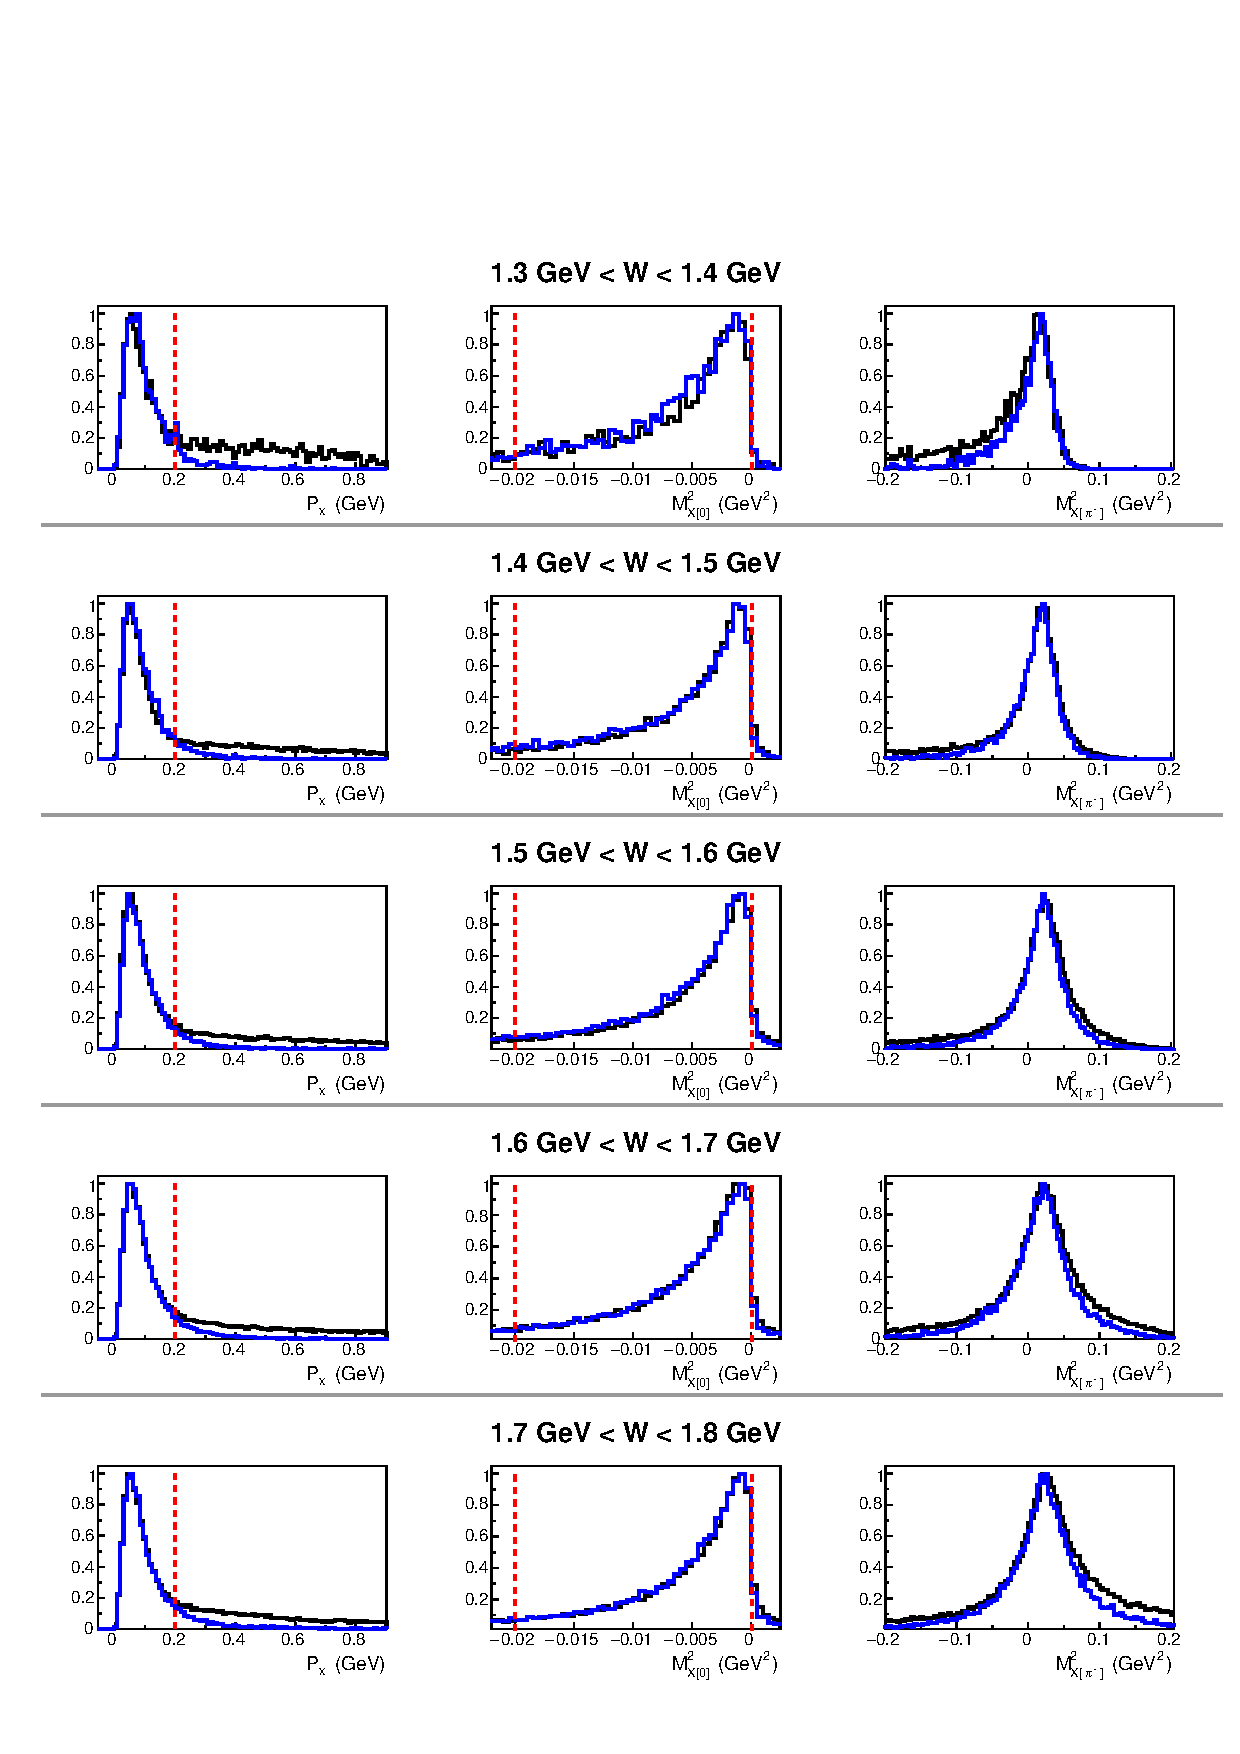
\includegraphics[width=14.5cm]{pictures/other_cuts/excl_cut/excl_top.pdf}}
\end{center}
\caption{\small Distributions of the quantities $P_{X}$ (left column), $M^{2}_{X[0]}$ (middle column), and $M^{2}_{X[\pi^{-}]}$ (right column) defined in Eq.~\eqref{eq:excl_top_quant} for experimental data (black curves) and Monte Carlo simulation (blue curves) for different 100-MeV-wide $W$ bins. Vertical red lines indicate the cuts applied for the selection of exclusive quasi-free events. All plotted quantities as well as the values of $W$ are calculated under the target-at-rest-assumption. All distributions are normalized to their maxima.}
\label{fig:excl_top}
\end{figure}



The quantities $P_{X}$ and $M^{2}_{X[0]}$ are unique for the fully exclusive topology, they can be calculated only if all final hadrons are registered. Although adding the missing mass squared $M_{X[\pi^{-}]}^{2}$ to this set seems not to provide any additional information, it is investigated in order to observe consistency with the $\pi^{-}$ missing topology, where the distribution of this quantity is the only source for developing a criterion for channel identification. See App.~\ref{app_mm_features} for details on features of missing mass distributions.


Distributions of the quantities $P_{X}$ (first column), $M^{2}_{X[0]}$ (second column), and $M_{X[\pi^{-}]}^{2}$ (third column) for five 100-MeV-wide bins\footnote[12]{The value of $W$ is calculated for the initial state under the target-at-rest-assumption by $W = \sqrt{(P_{e}^{\mu} + P_{p}^{\mu}- P_{e'}^{\mu})^{2}}$.} in $W$ are shown in Fig.~\ref{fig:excl_top} both for the experimental data (black curves) and reconstructed Monte Carlo events (blue curves).

The quantity $P_{X}$ (first column in Fig.~\ref{fig:excl_top}) is the missing momentum of the initial proton calculated under the target-at-rest-assumption, therefore the blue curves stand for the Fermi momentum (simulated according to Bonn potential~\cite{Machleidt:1987hj}) convoluted with the detector resolution, whereas the black ones correspond to the experimental momentum of initial proton, mixed with the FSI effects, contributions from background channels, and the detector resolution. As seen in the left column of Fig.~\ref{fig:excl_top}, the simulated distributions perfectly match the experimental ones for $P_{x} < 0.2$~GeV, while for $P_{x} > 0.2$~GeV the simulation underestimates data. Such behavior is mostly related to the fact that relative contributions from FSI, which were not included into the Monte Carlo simulation, turn out to be the most significant outside of the peak region. The background channels, being not included into the Monte Carlo as well, also contribute to this mismatch, but as mentioned above their contribution is minor.
The value  $P_{x} = 0.2$~GeV (marked by the red dashed lines in each plot in the left column) was chosen as a criterion for the selection of events in quasi-free kinematics. Thus, experimental events located at the left side of this line correspond to the reaction in the quasi-free regime, while events at the right side correspond mostly to ``disturbed" kinematics with great impact of FSI.

\begin{figure}[!ht]
\begin{center}
\framebox{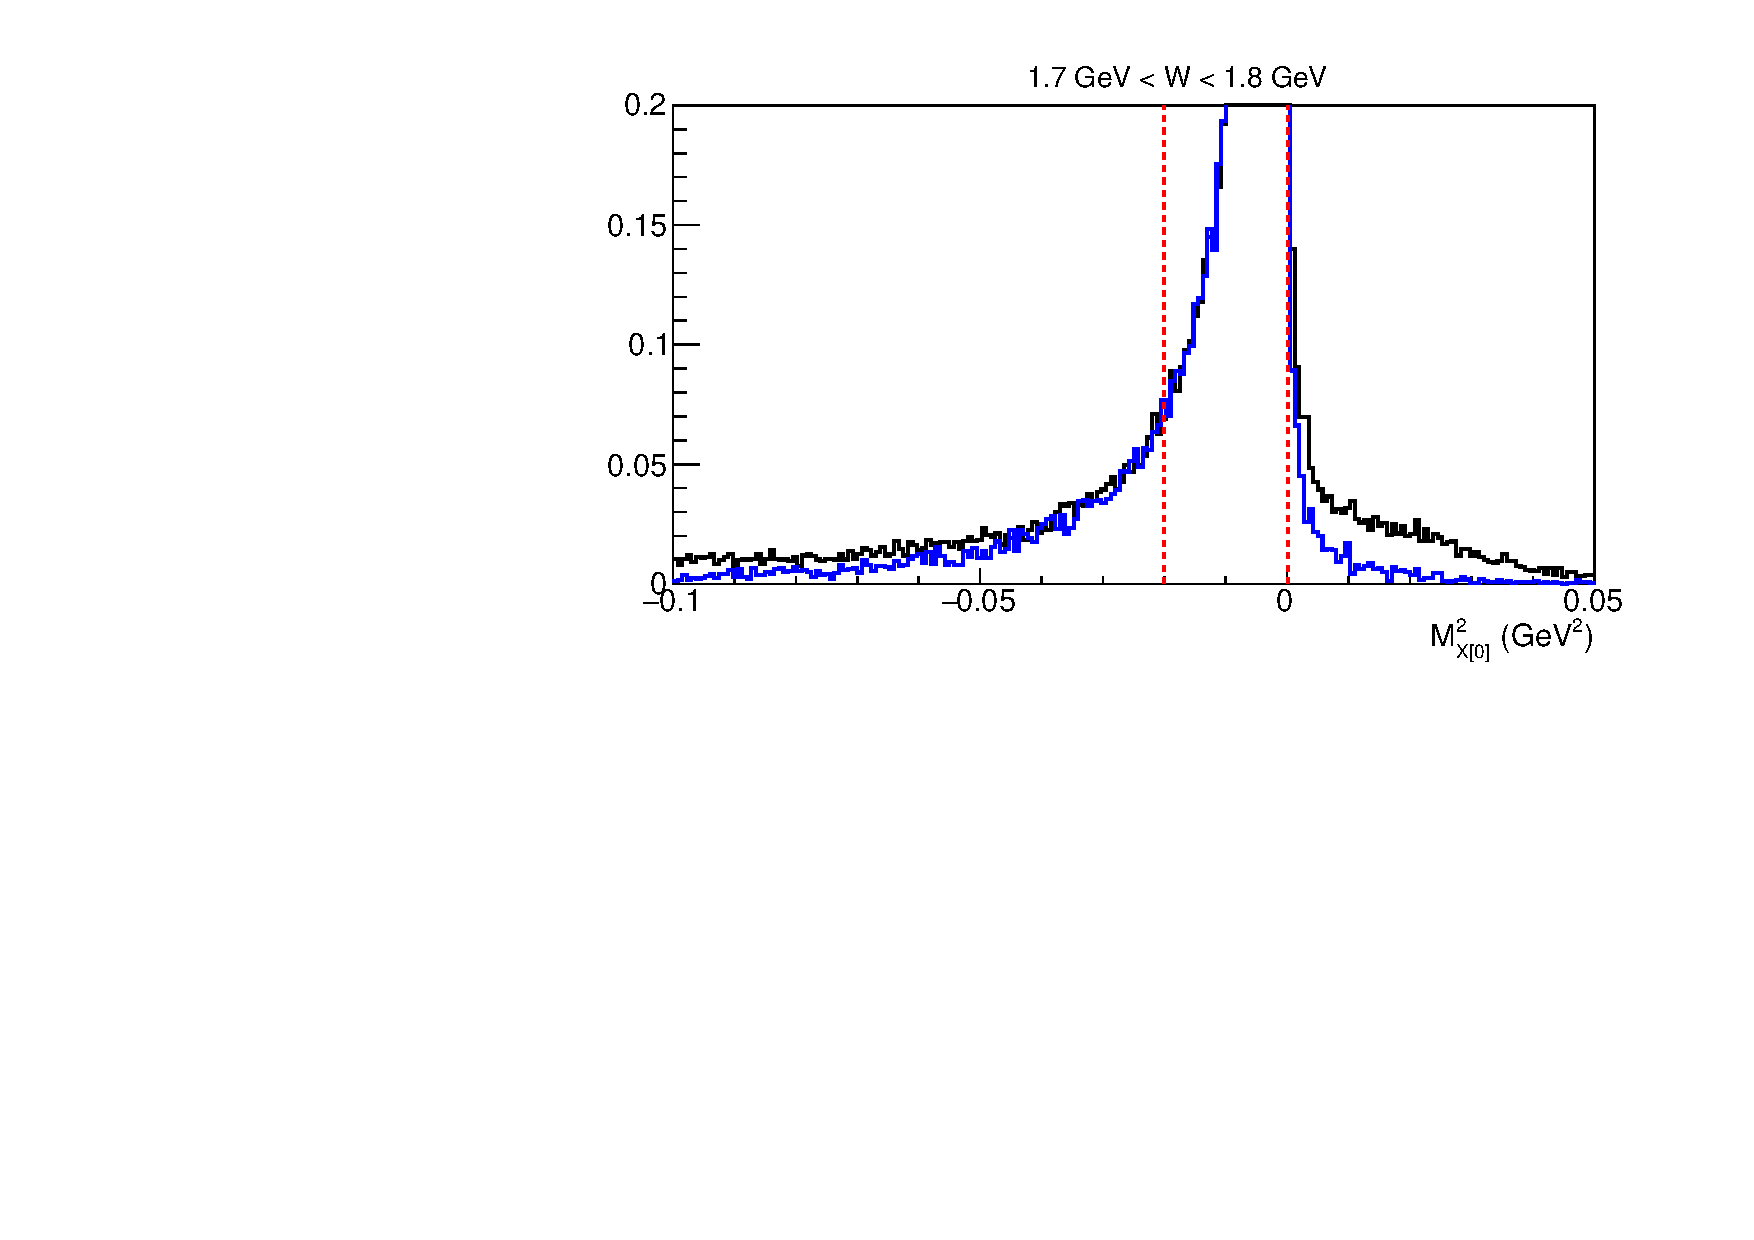
\includegraphics[width=13.1cm]{pictures/other_cuts/excl_cut/mm_0_zoomed.pdf}}
\end{center}
\caption{\small Distributions of the missing mass squared $M^{2}_{X[0]}$ for experimental data (black curves) and Monte Carlo simulation (blue curves) zoomed at the foot. Vertical red lines indicate the applied cut. The mismatch between data and simulation originates from FSI effects at the left and three-pion background at the right. The example is given for 1.7~GeV $< W <$ 1.8~GeV, where the latter is greatest over the whole $W$ range. The agreement between data and simulation within the cut boundaries is better shown in Fig.~\ref{fig:excl_top} (middle column).}
\label{fig:mm_0_zoomed}
\end{figure}


The distributions of the quantity $M^{2}_{X[0]}$ shown in the middle column in Fig.~\ref{fig:excl_top} deserve more attention. As demonstrated in Refs.~\cite{Fed_an_note:2017,Fed_paper_2018} and here in App.~\ref{app_mm_features}, in free proton experiments this quantity forms a very narrow peak at zero position barely affected either by radiative effects or by detector resolution. An admixture from the three-pion background, if present in the analyzed event sample, forms then an additional peaked structure at $m_{\pi}^{2}$ well-separated from the main distribution peak. Meanwhile, in this analysis $M^{2}_{X[0]}$, being calculated under the target-at-rest-assumption, loses its thinness and acquires the smearing (mostly left-sided), which is well-reproduced by the Monte Carlo simulation.

In order to clean up the sample of exclusive events, the cut on the missing mass squared $M^{2}_{X[0]}$ was also applied as complimentary to the cut on the missing momentum. This cut is shown in Fig.~\ref{fig:excl_top} (middle column) by the vertical red dashed lines. The plots in the middle column are zoomed near the peak to demonstrate good agreement between the data and the simulation within the cut limits. The behavior of $M^{2}_{X[0]}$ in a wider range is shown in Fig.~\ref{fig:mm_0_zoomed}, where the distributions are zoomed at the foot. As seen, outside the cut boundaries there is a mismatch between the data and simulation, which originates from FSI effects at the left and the contribution from the three-pion background at the right. The latter forms a peaked structure around $m_{\pi}^{2}$ ($\sim$0.02~GeV$^{2}$), which is more smeared compared to the free proton case due to the target-at-rest-assumption and FSI disturbances. The example is given for high $W$ to observe the greatest background admixture over the investigated $W$ range.

The three-pion background in this topology is considered to be fully eliminated by the described above cuts on the missing momentum $P_{X}$ and the missing mass squared $M^{2}_{X[0]}$.


The right column in Fig.~\ref{fig:excl_top} stands for the missing mass squared $M_{X[\pi^{-}]}^{2}$ defined by Eq.~\eqref{eq:excl_top_quant} under the target-at-rest-assumption, thus being Fermi smeared. The observed mismatch between the measured and simulated distributions is $W$-dependent and caused mostly by the FSI effects. 
\begin{figure}[!ht]
\begin{center}
\framebox{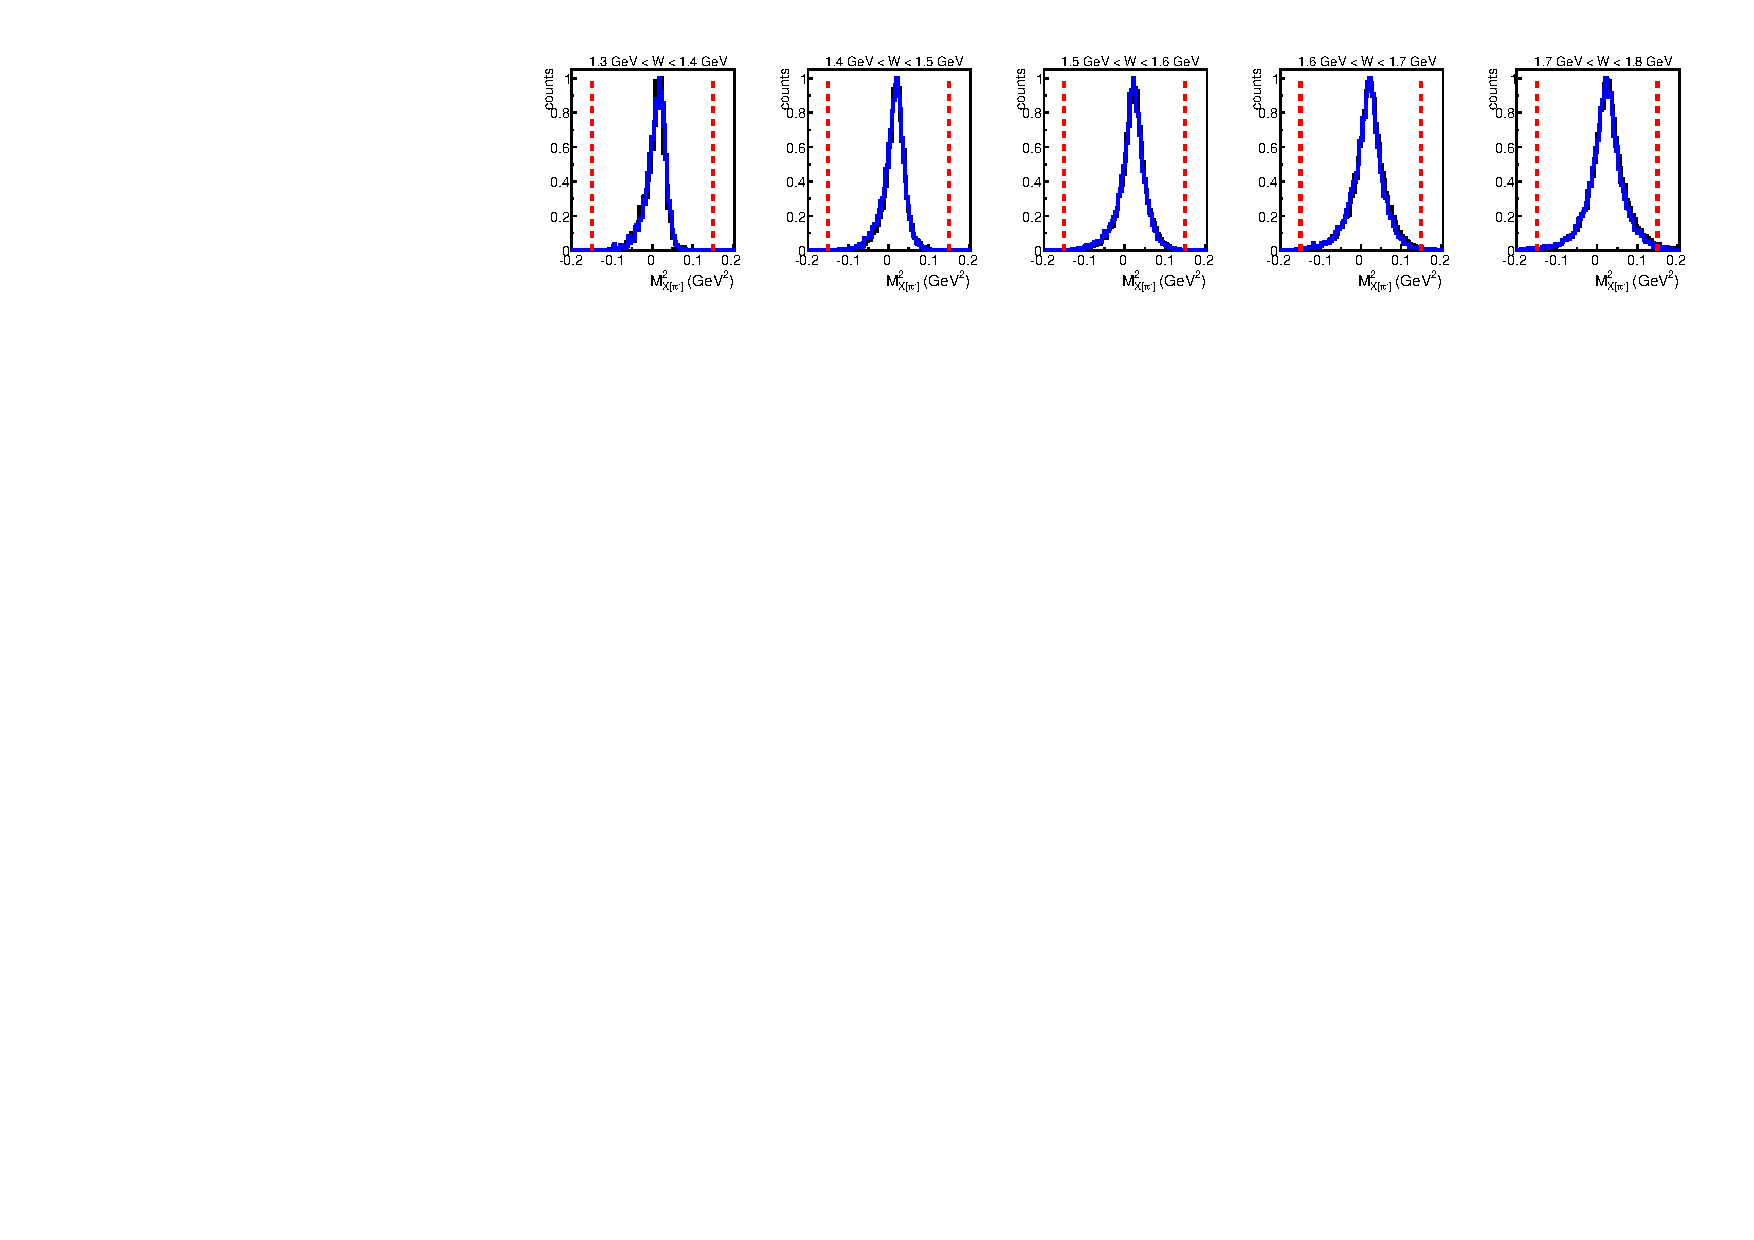
\includegraphics[width=\textwidth]{pictures/other_cuts/excl_cut/excl_top_aft_cut.pdf}}
\end{center}
\caption{\small Distributions of the missing mass squared $M^{2}_{X[\pi^{-}]}$ defined in Eq.~\eqref{eq:excl_top_quant} for the fully exclusive topology plotted for selected quasi-free exclusive events for experimental data (black curves) and Monte Carlo simulation (blue curves). The comparison is shown for different 100-MeV-wide $W$ bins. The quantity $M^{2}_{X[\pi^{-}]}$ as well as the values of $W$ are calculated under the target-at-rest-assumption. The vertical red lines show the applied cuts. All distributions are normalized to their maxima. See text for details. }
\label{fig:excl_top_aft}
\end{figure}

Figure~\ref{fig:excl_top_aft} shows the distributions of the missing mass squared $M_{X[\pi^{-}]}^{2}$ plotted for quasi-free exclusive events selected by the cuts on missing momentum $P_{x}$ and missing mass squared $M^{2}_{X[0]}$. The distributions for the experimental (black curves) and reconstructed Monte Carlo (blue curves) events perfectly match each other in all $W$ subranges, which demonstrates the reliability of quasi-free exclusive event selection as well as the fact that effects of the target motion are correctly implemented into the simulation. The vertical red lines in Fig.~\ref{fig:excl_top_aft} correspond to the additional cut that was applied on the missing mass squared $M_{X[\pi^{-}]}^{2}$.

Although in the fully exclusive topology the four-momentum of the $\pi^{-}$ is measured precisely within the detector resolution, it is not used in the subsequent calculation of kinematic variables for the cross section extraction. The measured four-momentum is instead replaced by the one that is calculated as missing ($P_{\pi^{-}~miss}^{\mu}$ in Eq.~\eqref{eq:excl_top_quant}) and thus is Fermi smeared. This is done to imitate the event selection in the main $\pi^{-}$ missing topology in order to treat events in both topologies identically. 


\subsection{$\pi^{-}$ missing topology}
\label{Sect:excl_cut_pim_miss}

In the $\pi^{-}$ missing topology the quantities $P_{X}$ and $M^{2}_{X[0]}$ defined in Eq.~\eqref{eq:excl_top_quant} are not available due to the incomplete knowledge about the final state, and $M_{X[\pi^{-}]}^{2}$ is the only remaining quantity suitable for the selection of exclusive events in quasi-free kinematics. The distributions of this quantity are shown in Fig.~\ref{fig:main_top_mm2} for five 100-MeV-wide bins in $W$ for the experimental data (black curves) and the Monte Carlo simulation (blue curves). The comparison shown in this figure demonstrates again the $W$-dependent mismatch between data and simulation, which is different from that seen in the fully exclusive topology. The mismatch is mostly observed at the right side of the distribution peak and becomes discernible only for $W\gtrsim 1.5$~GeV.
\begin{figure}[!ht]
\begin{center}
\framebox{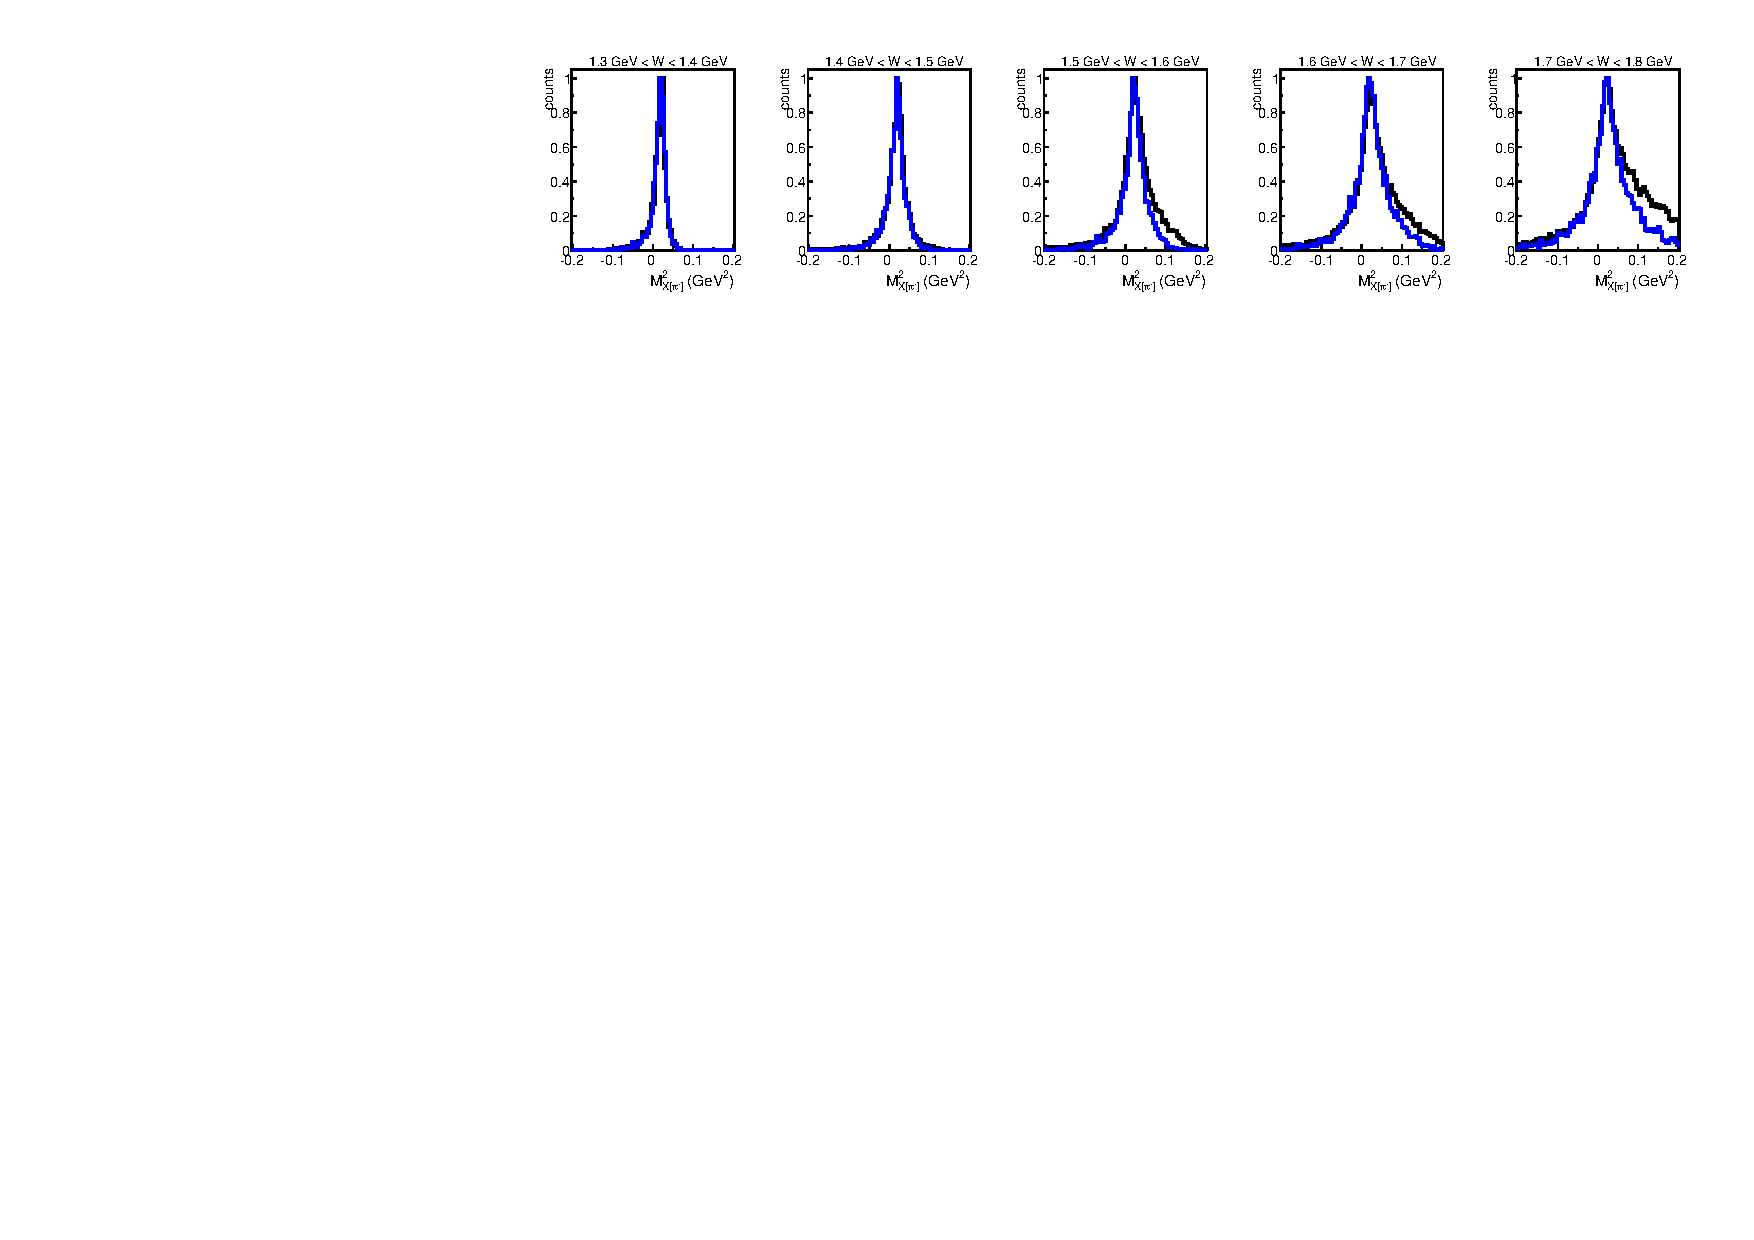
\includegraphics[width=16cm]{pictures/other_cuts/excl_cut/main_top_mm2.pdf}}
\end{center}
\caption{\small Distributions of the missing mass squared $M^{2}_{X[\pi^{-}]}$ defined in Eq.~\eqref{eq:excl_top_quant} for the $\pi^{-}$ missing topology plotted before the selection of quasi-free exclusive events for experimental data (black curves) and Monte Carlo simulation (blue curves). The comparison is shown for different 100-MeV-wide $W$ bins. The quantity $M^{2}_{X[\pi^{-}]}$ as well as the values of $W$ are calculated under the target-at-rest-assumption. All distributions are normalized to their maxima. See text for details. }
\label{fig:main_top_mm2}
\end{figure}

The similar analysis~\cite{Fed_an_note:2017} carried out for the same beam energy but off a free proton target did not reveal any substantial discrepancies between the experimental and simulated distributions of the quantity $M_{X[\pi^{-}]}^{2}$; they are shown to be in a very good agreement for all $W$ values. Figure~\ref{fig:excl_top_aft} plotted for selected exclusive quasi-free events in the fully exclusive topology in turn proves that the Monte Carlo simulation incorporates effects of the target motion correctly. Therefore, the discrepancy between data and simulation observed in Fig.~\ref{fig:main_top_mm2} is attributed mainly to the FSI effects, which are not included into the simulation.

This mismatch between data and simulation together with the fact that in the $\pi^{-}$ missing topology the quantity $M_{X[\pi^{-}]}^{2}$ is the only one available for the channel identification makes the task of selecting events in quasi-free kinematic rather challenging. To accomplish this goal, a special procedure was developed. This procedure is described below. 

To select events in quasi-free kinematics properly, the following quantity is analyzed.%\vspace{-1em}
\begin{equation}
 M_{X[\pi^{-}]}=\sqrt{|M_{X[\pi^{-}]}^{2}|}=\sqrt{|[P_{\pi^{-}~miss}^{\mu}]^{2}|}=\sqrt{|[P_{e}^{\mu} + P_{p}^{\mu}- P_{e'}^{\mu}- P_{p'}^{\mu}-  P_{\pi^{+}}^{\mu}]^{2}|}.\label{eq:main_top_mm_nosq}
\end{equation}\vspace{-1em}

%\afterpage{\clearpage}
\begin{figure}[!ht]
\begin{center}
\framebox{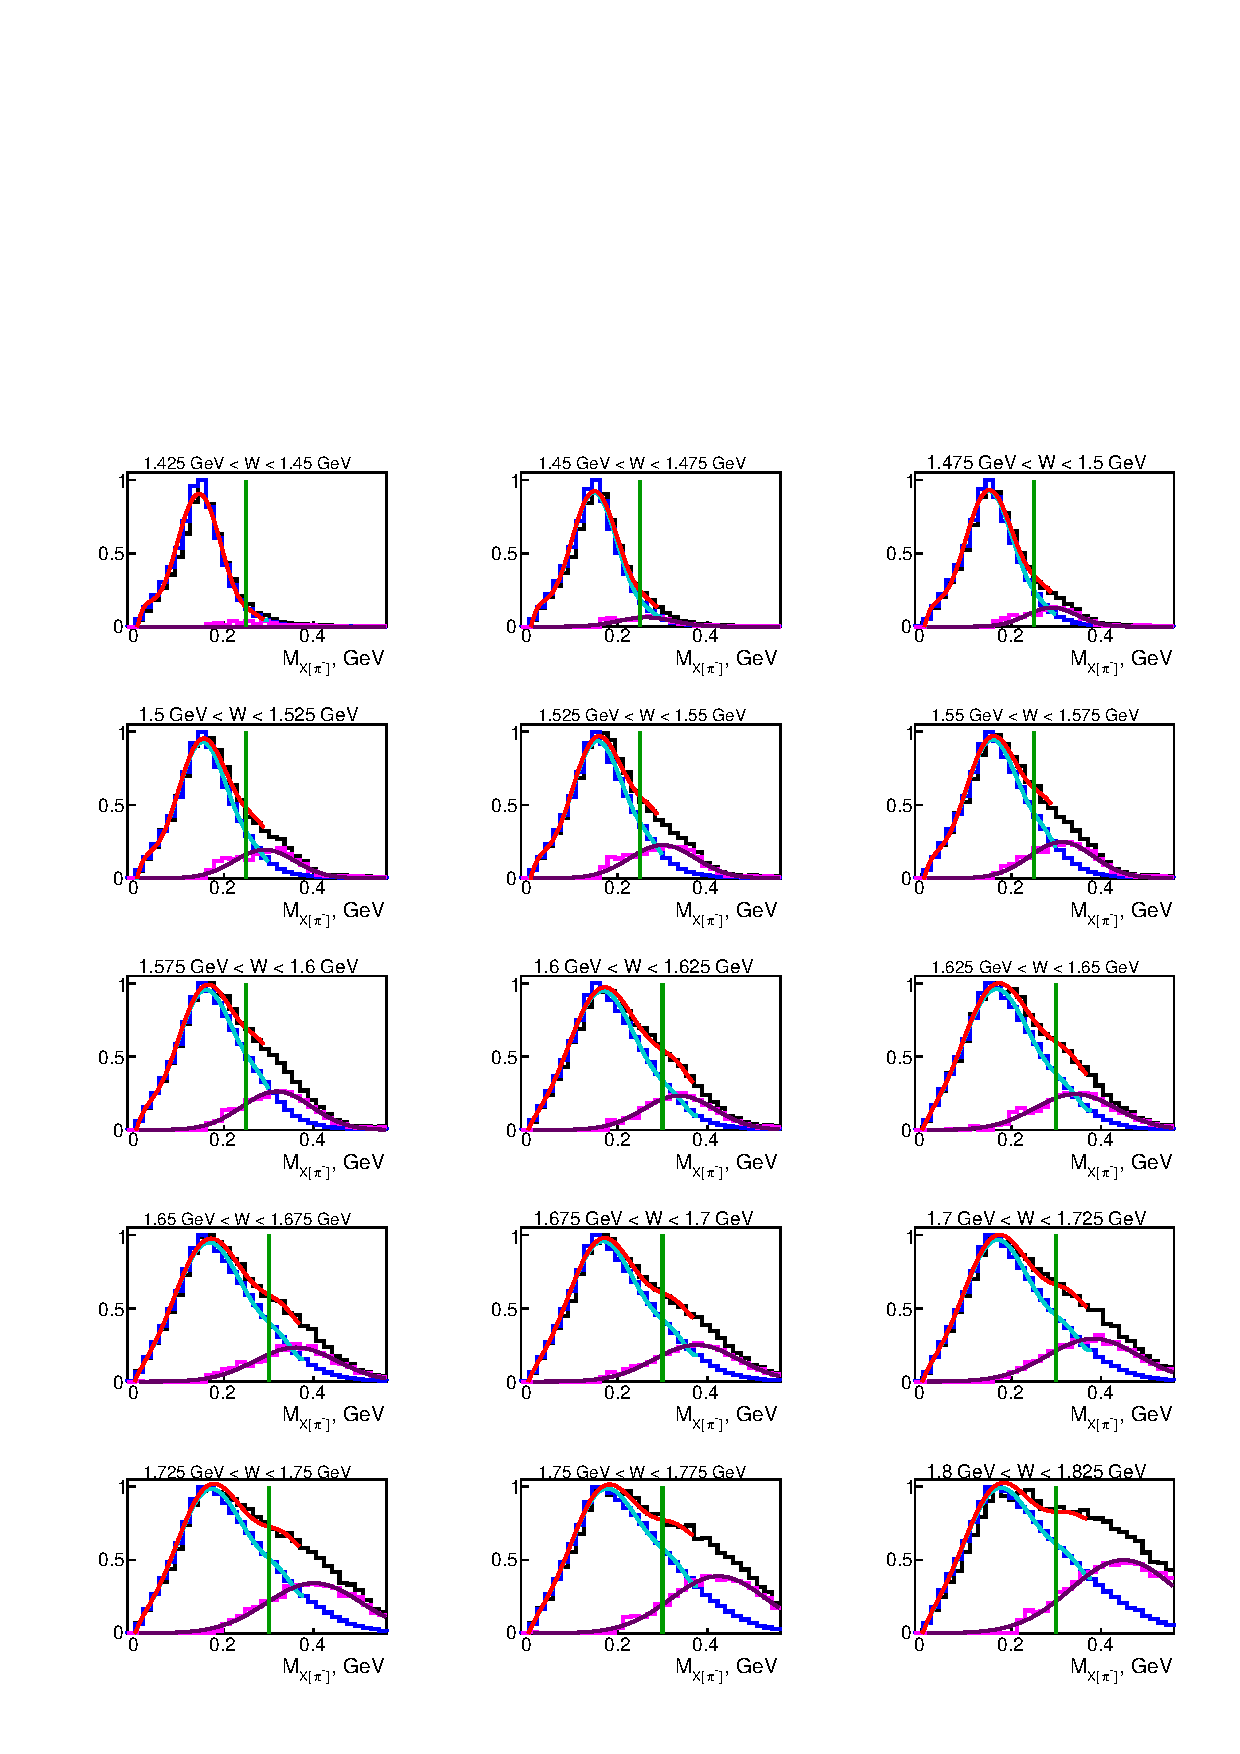
\includegraphics[width=15.5cm]{pictures/other_cuts/excl_cut/main_top_mm_fsi_corr2.pdf}}
\end{center}
\caption{\small Distributions of the quantity $M_{X[\pi^{-}]}$ (defined by  Eq.~\eqref{eq:main_top_mm_nosq}) in different 25-MeV-wide $W$ bins for experimental data (black histograms), Monte Carlo simulation (blue histograms), and their difference (magenta histograms). The explanation of the fit curves is given in the text. Green vertical lines correspond to the position of the cut that is intended to select quasi-free events. This cut is applied to the reconstructed Monte Carlo events as well.}
\label{fig:main_top_mm_fsi_corr}
\end{figure}
\clearpage

The distributions of the quantity $M_{X[\pi^{-}]}$ in different 25-MeV-wide $W$ bins are shown in Fig.~\ref{fig:main_top_mm_fsi_corr} for experimental data (black histograms) and for Monte Carlo simulation (blue histograms). Both are normalized to their maxima. The mismatch between data and simulation becomes discernible at $W\approx 1.5$~GeV, increases as $W$ grows and becomes large at $W\approx 1.8$~GeV. The magenta histogram stands for the difference between the black and blue histograms and thus represents the distribution of background events originated mainly from FSI effects. The green vertical lines correspond to the position of the cut that is intended to select quasi-free events. This cut is applied to the reconstructed Monte Carlo events as well. However, as seen in Fig.~\ref{fig:main_top_mm_fsi_corr}, one can hardly completely separate the quasi-free event sample from the FSI-background by tightening the cut: in this way the statistics of quasi-free events will be subject to significant reduction, while the background admixture will still not be completely eliminated. Therefore, it was decided to perform a so-called ``effective correction" of the FSI-background admixture, which includes the following steps.

\begin{itemize}
\item The distributions of $M_{X[\pi^{-}]}$ for the reconstructed Monte Carlo events (blue histograms) were fit by a ninth order polynomial in a slightly wider range than marked by the green cut lines. The results of the fit are shown in Fig.~\ref{fig:main_top_mm_fsi_corr} by the cyan curves.
\item The magenta background distributions were fit by Gaussians. The results of the fit are shown by the dark-magenta curves.
\item The cyan and dark-magenta curves were summed up to produce the red curve, which perfectly matches the black experimental histogram in each $W$ bin.
\item The following correction factor was determined in the left side of the green cut line,
\begin{equation}
 F_{fsi}(W) = \frac{\color{cyan}{area~under~the~cyan~curve}}{\color{red}{area~under~the~red~curve}} \leq 1.\label{eq:fsi_corr_fact}
\end{equation}\label{eq:fsi_corr}\vspace{-1em}
\item In each $W$ bin the experimental event yield in the $\pi^{-}$-missing topology is multiplied by the factor $F_{fsi}$, which serves as an effective correction due to the remaining admixture of the FSI-background events.
\end{itemize}


The factor $F_{fsi}$ is assumed to be only $W$ dependent as it was found that it does not demonstrate any $Q^{2}$ dependence, and the dependence on the final hadron variables is neglected due to the statistics limitation. The value of $F_{fsi}$ varies from $\sim$0.97 to $\sim$0.93 in the $W$ range from 1.4625~GeV to 1.8125~GeV, while for $W < 1.4625$~GeV $F_{fsi}=1$ as the correction there is not needed.


Note that the exclusivity cut shown in Fig.~\ref{fig:main_top_mm_fsi_corr} accompanied by the corresponding correction cares for all other possible effects that along with the FSI effects may contribute to the mismatch between the data and the simulation in this topology (including the three-pion background).


\setcounter{chapter}{2}
\chapter{Cross section calculation}
\label{Sect:cr_sect}



\section{$W$-smearing and boundary blurring of the $Q^{2}$ versus $W$ distribution}
\label{Sect:smearing_blurring}

The smearing of the invariant mass $W$ has the same origin as the smearing of the missing mass, which is already discussed in Sect.~\ref{Sect:excl_cut}, but since $W$ is the variable needed to describe the reaction (and the extracted cross section is binned in $W$), the issue of $W$-smearing requires special attention and, therefore, is separately addressed here.


For the process of double-pion electroproduction off the proton (as for any other exclusive process) the reaction's invariant mass can in general be determined in two ways, i.e. either from the initial particle  four-momenta\footnote[1]{Although the scattered electron is treated as a final particle, here it is classified as ``initial", since it defines the virtual photon, which in turn is attributed to the initial state.} ($W_{i}$) or from the final particle  four-momenta ($W_{f}$) as Eqs.~\eqref{W_fin_1} and~\eqref{W_fin_2} demonstrate. 


%\begin{equation}
\begin{eqnarray}
W_{i}&= & \sqrt{(P_{p}^{\mu}+P_{\gamma_{v}}^{\mu})^{2}} \label{W_fin_1} \\
W_{f}&= & \sqrt{(P_{\pi^{+}}^{\mu}+P_{\pi^{-}}^{\mu}+P_{p'}^{\mu})^{2}} \label{W_fin_2}
\end{eqnarray}
%\end{equation}

Here $P_{\pi^{+}}^{\mu}$, $P_{\pi^{-}}^{\mu}$, and $P_{p'}^{\mu}$ are the four-momenta of the final state hadrons, $P_{p}^{\mu}$ is the four-momentum of the initial proton and $P_{\gamma_{v}}^{\mu}=P_{e}^{\mu}-P_{e'}^{\mu}$ the four-momentum of the virtual photon with $P_{e}^{\mu}$ and $P_{e'}^{\mu}$ the four-momenta of the incoming and scattered electrons, respectively. 

To determine $W_{f}$, all final hadrons should be registered, while for the calculation of $W_{i}$ it is sufficient to register the scattered electron. The latter opportunity allows event samples with one unregistered final hadron, whose four-momentum is recovered via the missing mass technique, to be used. This approach allows for a significant increase of the analyzed statistics (see Sect.~\ref{Sect:excl_cut}).

In experiments off protons at rest $W_{f}$ and $W_{i}$ may differ due to the detector resolution and the radiative effects, which electrons undergo. In moving proton experiments one more aspect takes effect, i.e. in order to calculate $W_{i}$, one needs information about the target proton momentum ($P_{p}^{\mu}$), which is accessible only in the fully exclusive topology\footnote[2]{If the spectator nucleon momentum is not directly measured in the experiment. This was not an option in the analyzed ``e1e" experiment. }. Therefore, the value of  $W_{i}$ given by Eq.~\eqref{W_fin_1} turns out to be ill-defined, if one of the final hadrons is not registered. This brings us to the choice to either demand the registration of all final hadrons to determine $W_{f}$ (that reduces the flexibility of the analysis) or to work under a so-called ``target-at-rest-assumption", which assumes the initial proton to be at rest. In the last approach the value of $W_{i}$ appears to be smeared. This smeared value of the invariant mass is hereinafter denoted as $W_{sm}$. Meanwhile, the value $W_{f}$ corresponds to the true reaction invariant mass and, therefore, is denoted as $W_{true}$. It can be calculated only in the fully exclusive topology.

If a smeared value $W_{sm}$ is used to describe the reaction, the extracted cross sections turned out to be convoluted with a function that is determined by the Fermi motion of the initial proton~\cite{Skorodumina:2015rea,twopeg-d}. To retrieve the non-smeared observable, a correction that unfolds this effect should be applied to the cross sections.


Beside the $W$-smearing, the Fermi motion of the target proton is also responsible for the boundary blurring of the $Q^{2}$ versus $W$ distribution\footnote[3]{This issue is addressed in more details in Ref.~\cite{twopeg-d}}. This happens because the experiment off the moving proton with fixed laboratory beam energy is equivalent to that off the proton at rest performed with altered effective beam energy~\cite{twopeg-d}. The boundaries of the $Q^{2}$ versus $W$ distribution, however, are beam energy dependent. Therefore, the distribution edges, being sharp and distinct in the proton at rest experiment, become blurred in the experiment off a moving proton.


%The issue of $W$-smearing is closely related to a problem of blurring of the $Q^{2}$ versus $W$ distribution boundaries in reactions off moving protons\footnote[3]{This issue is addressed in more details in Ref.~\cite{twopeg-d}}. 
%In electron scattering experiments the fixed beam energy imposes kinematic limits on the maximal achievable values of $W$ and $Q^2$.  The kinematic limitations are usually more strongly restricted by the experimental conditions, i.e. by the limitations on the polar angle and minimal detectable energy of the scattered electron. The formulae that give the shapes of $Q^{2}$ versus $W$ distribution edges for various restriction types are given in Ref.~\cite{twopeg-d}.

%The edges of the $Q^2$ versus $W$ distribution are beam energy dependent. As demonstrated in Ref.~\cite{twopeg-d}, the experiment off the moving proton with fixed laboratory beam energy is equivalent to that off the proton at rest performed with altered effective beam energy. Therefore, the distribution edges, being sharp and distinct in the proton at rest experiment, become blurred in the experiment off the moving proton.

The blurring, however, affects only the edges of $Q^{2}$ versus $W_{true}$ distribution, where $W_{true}$ is the true reaction invariant mass given by Eq.~\eqref{W_fin_2}, since $W_{true}$ accounts for the target motion and, therefore, for the alteration of the effective beam energy. If the smeared value $W_{sm}$, calculated by Eq.~\eqref{W_fin_1} under the target-at-rest-assumption, is used instead, the distribution edges are not subject to the blurring because the fixed value of the laboratory beam energy is used in calculations.

\begin{figure}[htp]
\begin{center}
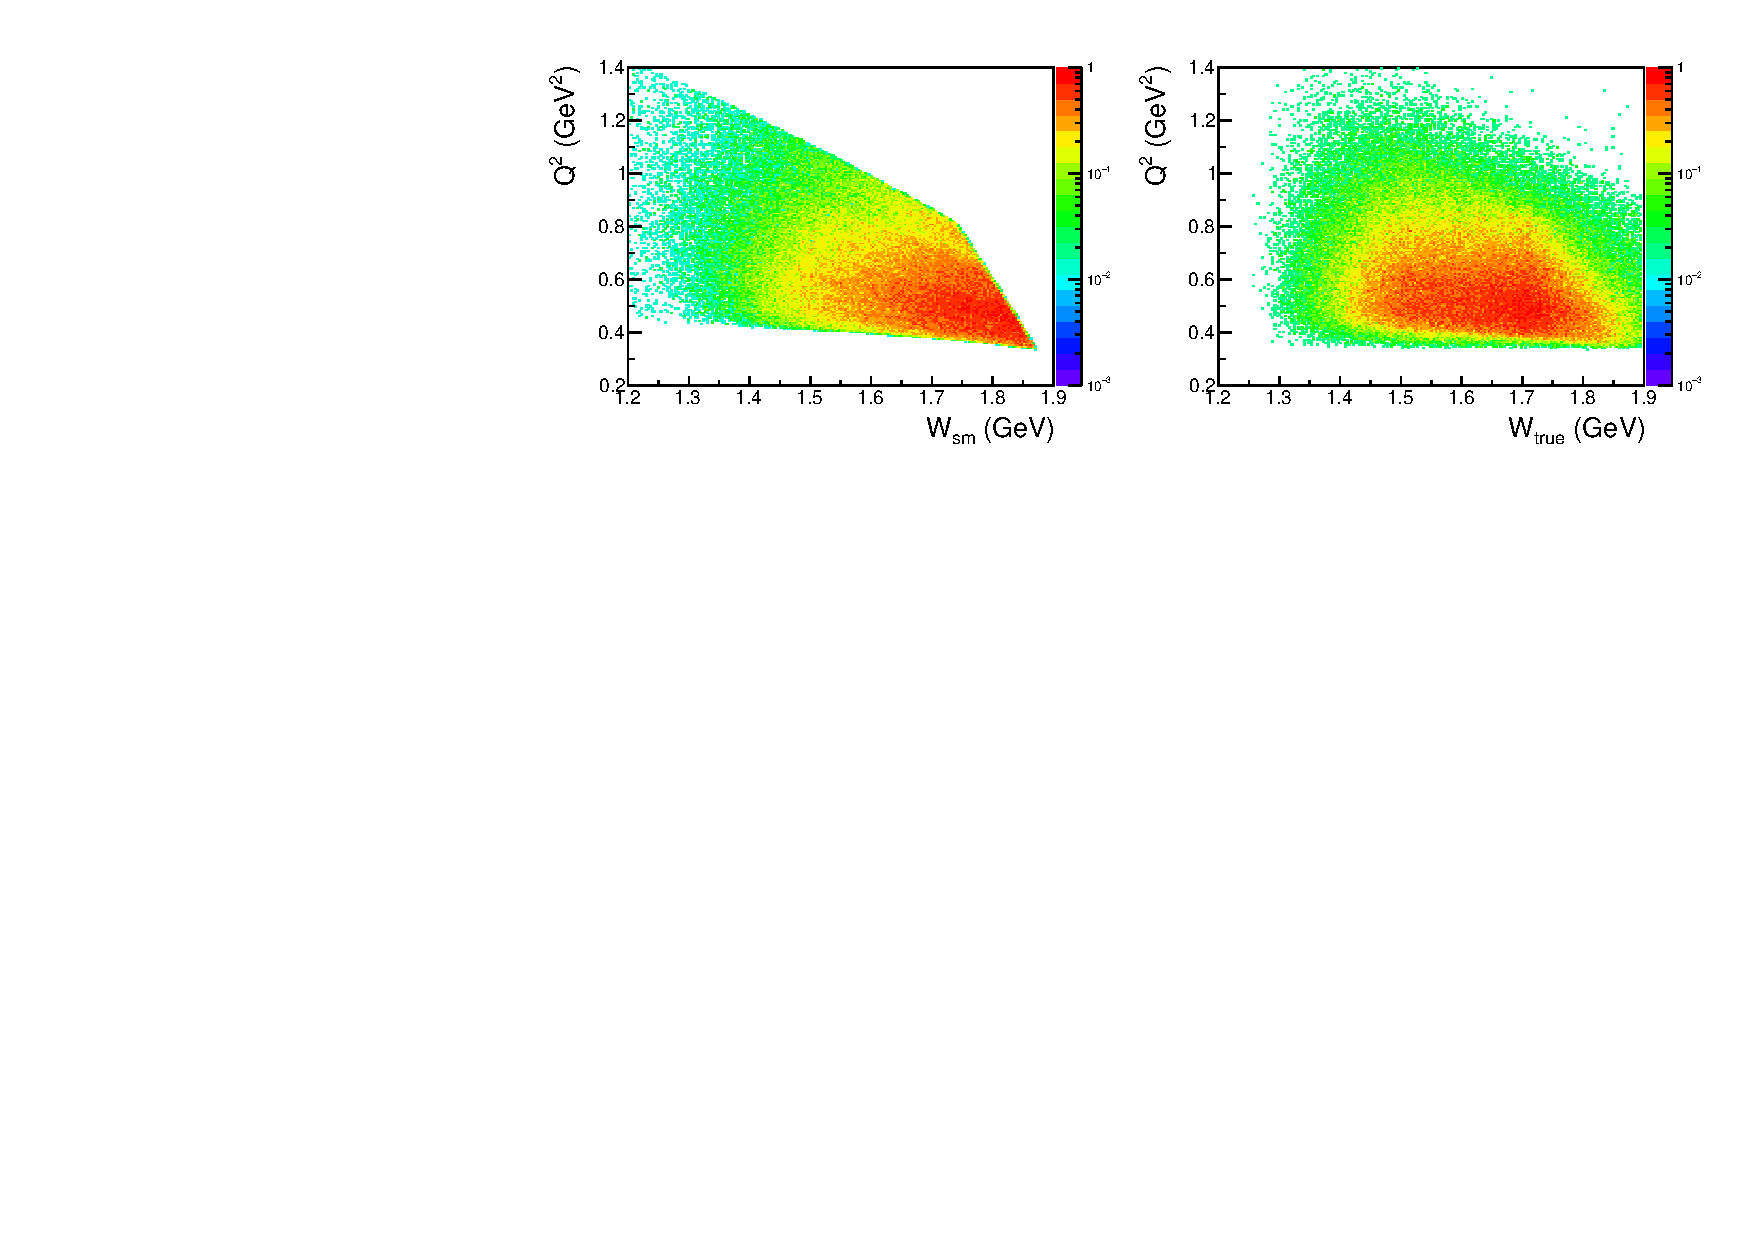
\includegraphics[width=16.5cm]{pictures/cross_section/blurring.pdf}
\caption{\small Experimental $Q^2$ versus $W$ distributions for $W_{sm}$ (left) and $W_{true}$ (right) plotted for the fully exclusive topology. The boundaries of the left distribution are sharp, since the $W_{sm}$ is calculated under the target-at-rest-assumption and the fixed value of the laboratory beam energy is used in calculations. The boundaries of the right distribution are blurred, since the calculation of $W_{true}$ accounts for the target proton motion and therefore for the alteration of the effective beam energy of the experiment.} \label{fig:blurring}
\end{center}
\end{figure}

This situation is illustrated in Fig.~\ref{fig:blurring}, where the $Q^2$ versus $W$ distributions are shown for $W_{sm}$ (left) and $W_{true}$ (right). These distributions are plotted for the fully exclusive topology only, since it allows for the determination of both $W_{sm}$ and $W_{true}$. The distributions, therefore, contain only a small portion of the total analyzed statistics. The boundaries of the left distribution are sharp, since the $W_{sm}$ is calculated assuming the fixed laboratory beam energy and the target at rest. The boundaries of the right distribution are blurred, since the calculation of $W_{true}$ accounts for the target proton motion and, therefore, for the alteration of the effective beam energy of the experiment.


The event yield in the blurred region suffers from depletion of events (compared to that for the case of fixed beam energy and sharp distribution edges). To estimate this effect, one should know the function that describes the alteration of the effective beam energy. This function is in turn determined by the target proton momentum distribution. The cross sections extracted in the blurred region need a special correction, otherwise they will suffer from the underestimation.



The situation described above offers two options, i.e. to use either $W_{sm}$ or $W_{true}$ to describe the reaction. The former opportunity leads to the need to apply a correction that unfolds the cross section smearing, while the latter requires the correction due to the blurring effect. The first option was chosen in this analysis because it has the advantage of using the $\pi^{-}$ missing topology that accumulates the majority of the experimentally available statistics. 

Thus, to calculate the cross section in this analysis, events are binned in $W_{sm}$. Note, however, that the corresponding $W$ points on the chosen $W_{sm}$ grid (see Sect.~\ref{Sect:binning}) are then treated as actual $W$-values where the cross section is eventually reported. However, the cross section values assigned to these $W$ points is treated as distorted. The necessary correction to the cross section is based on the TWOPEG-D event generator~\cite{twopeg-d}, which offers a proper Monte Carlo simulation of the double-pion electroproduction off moving protons. This correction is described in Sect.~\ref{Sect:fermi_corr}.




%====================================

\section{Lab to CMS transformation}
\label{Sect:lab_cms}

Once the quasi-free double-pion events are selected as described in Chapter~\ref{Sect:select}, the laboratory four-momenta of all final particles are known: they are either registered or calculated as missing. These four-momenta are then used for the calculation of the kinematic variables, which are introduced in Sect.~\ref{Sect:kin_var}. The cross sections meanwhile are extracted in the center-of-mass frame of the {\em virtual photon -- initial proton} system (CMS). Therefore, to calculate the kinematic variables, the four-momenta of all particles need to be transformed from the laboratory system (Lab) to the CMS.

The CMS is uniquely defined as the system, where the initial proton and the photon move towards each other with the $z_{CMS}$-axis along the photon and the net momentum equal to zero. However, the procedure of the Lab to CMS transformation differs depending on the specificity of the reaction initial state (real or virtual photons, at rest or moving target). Figure~\ref{fig:lab_to_CMS} illustrates three options\footnote[4]{The fourth option of the reaction off the moving proton induced by the real photons is not shown.} for the experimental specification of the reaction initial state.%Therefore, the electroproduction experiment conducted on the moving in deuterium proton requires different procedure of Lab-to-CMS transformation than that performed on the proton at rest. 

 
\begin{figure}[!ht]
\begin{center}
\framebox{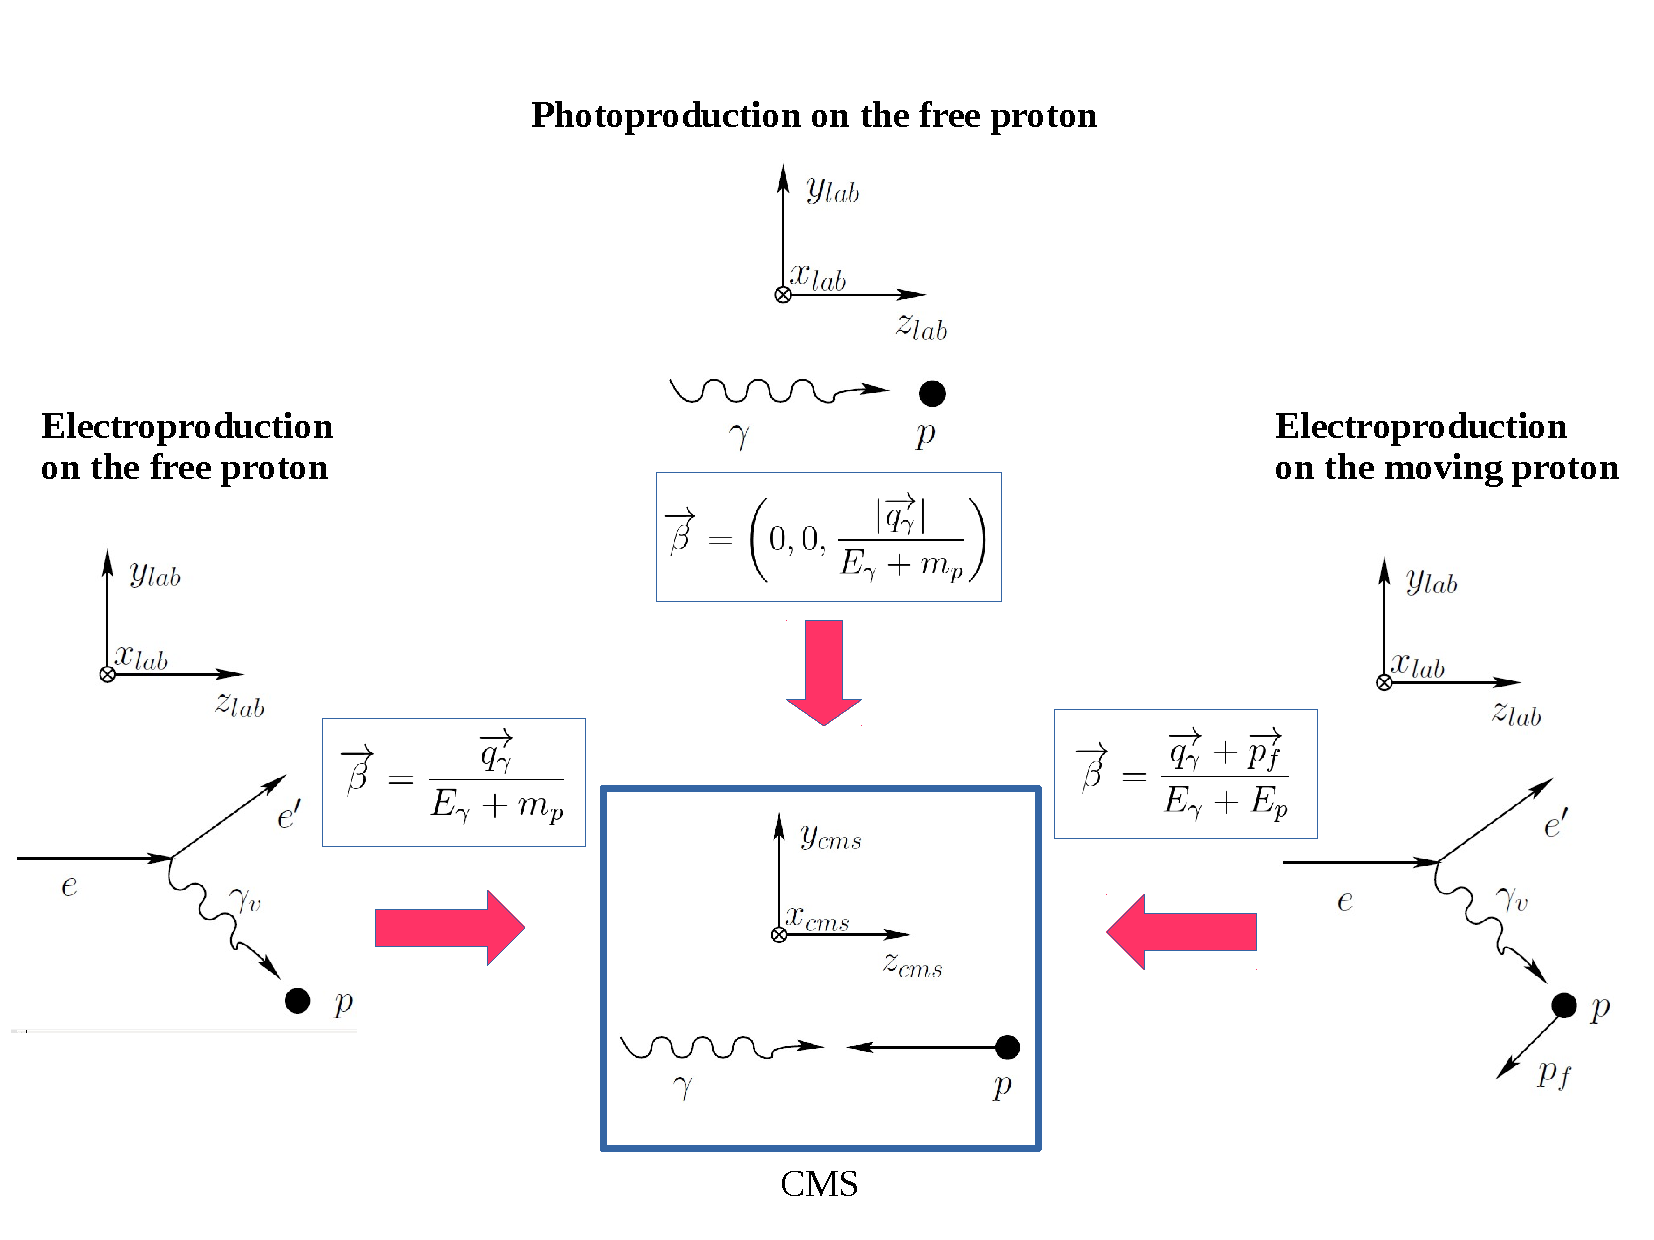
\includegraphics[width=13cm]{pictures/cross_section/lab_cms_trans2.pdf}}
\end{center}
\caption{\small  Illustration of three options for the experimental specification of the reaction initial state. Here $m_{p}$ is the proton mass, $\vec q_{\gamma}$ and $E_{\gamma}$ are the three-momentum and the energy of the interacting photon, respectively, while $p_{f}$ is the Fermi momentum of the target proton.}
\label{fig:lab_to_CMS}
\end{figure}


The correct procedure of the Lab to CMS transformation for an electroproduction experiment off a moving target (bottom right illustration in Fig.~\ref{fig:lab_to_CMS}) can be subdivided into two major steps.

\begin{enumerate}
\item First, one needs to perform the transition to the auxiliary system, where the target proton is at rest, while the incoming electron moves along the $z$-axis. This system is called ``quasi-Lab", since the initial conditions of the reaction in this frame imitate those existing in the Lab system in the case of the free proton experiment. The recipe of the Lab to quasi-Lab transformations is given in detail in Ref.~\cite{twopeg-d}.

\item Then, the quasi-Lab to CMS transformation should be performed by the standard method used for an electroproduction experiment off a proton at rest~\cite{Fed_an_note:2017} (bottom left illustration in Fig.~\ref{fig:lab_to_CMS}). Further details are given in App.~\ref{app_lab_cms_trans}.
\end{enumerate}


To perform the first step of this procedure (Lab to quasi-Lab transformation), one should be aware of the initial proton momentum for each reaction event~\cite{twopeg-d}. In this analysis, however, this information is available only in the fully exclusive topology, while the main $\pi^{-}$ missing topology lacks this information. This situation brings us to the impossibility to perform the correct Lab to CMS transformation for the majority of events. Therefore, in this analysis the procedure of Lab to CMS transformation for an electroproduction experiment off a proton at rest~\cite{Fed_an_note:2017} is used (bottom left illustration in Fig.~\ref{fig:lab_to_CMS}). The procedure is described in App.~\ref{app_lab_cms_trans}. This is done for both fully-exclusive and main $\pi^{-}$ missing topologies for consistency.

This approximation in the Lab to CMS transformation introduces a systematic inaccuracy to the extracted cross sections. A correction for this effect is included into the procedure of unfolding the effects of the target motion (see Sect.~\ref{Sect:fermi_corr}).






\clearpage


\section{Kinematic variables}
\label{Sect:kin_var}


When the four-momenta of all particles are defined and transformed to the CMS, one can calculate the kinematic variables that describe the reaction $ep(n) \rightarrow e'p'(n')\pi^{+}\pi^{-}$. For the description of the reaction initial state two variables are needed. In this study they are chosen in the following way: the invariant mass $W$, which is calculated according to Eq.~\eqref{W_fin_1}, and the photon virtuality $Q^{2}$, which is defined as
\begin{eqnarray}
Q^{2}= & -(P_{\gamma_{v}}^{\mu})^{2} = -(P_{e}^{\mu}-P_{e'}^{\mu})^{2}, \label{eq:q2} 
\end{eqnarray}
where $P_{\gamma_{v}}^{\mu}$ is the four-momentum of the virtual photon, while $P_{e}^{\mu}$ and $P_{e'}^{\mu}$ the four-momenta of the incoming and scattered electrons, respectively. 


%In the electron scattering process the variables $W$ and $Q^{2}$ are also present besides the hadronic variables. Thus the electron scattering cross section for double-pion electroproduction should be seven-fold differential and may be written as $\frac{d^{7}\sigma}{dWdQ^{2}d^{5}\tau}$, where $d^{5}\tau$ is five-dimensional phase-space differential.

The three-body final hadron state is unambiguously determined by five kinematic variables~\cite{Fed_an_note:2017}, and there are several options for their choice. The following generalized set of variables is used in this analysis\footnote[5]{More details on the organization of the reaction phase-space can be found in App.~\ref{app_ph_space}.}:\vspace{-0.5em}

\begin{itemize}
\item invariant mass of the first pair of the hadrons $M_{h_{1}h_{2}}$,\vspace{-0.4em}
\item invariant mass of the second pair of the hadrons $M_{h_{2}h_{3}}$,\vspace{-0.4em}
\item the first particle solid angle $\Omega_{h_{1}} = (\theta_{h_{1}}, \varphi_{h_{1}})$, and\vspace{-0.4em}
\item the angle $\alpha_{h_{1}}$ between the two planes (i) defined by the three-momenta of the virtual photon (or initial proton) and the first final hadron and (ii) defined by the three-momenta of all final hadrons\footnote[6]{Note that the three-momenta of the $\pi^{+}$, $\pi^{-}$, $p'$ are in the same plane, since in the CMS their total three-momentum has to be equal to zero.}.\vspace{-0.5em}
\end{itemize}

The cross sections in this analysis are obtained in three sets of variables depending on various assignments for the first, second, and third final hadrons:\vspace{-0.5em}
\begin{itemize}
\item[1.] [$p'$, $\pi^{+}$, $\pi^{-}$]
$M_{p'\pi^{+}}$, $M_{\pi^{+}\pi^{-}}$, $\theta_{p'}$~,~$\varphi_{p'}$~,~$\alpha_{p'}$~~(or $\alpha_{[pp'][\pi^{+}\pi^{-}]}$),\vspace{-0.25em}

\item[2.] [$\pi^{-}$, $\pi^{+}$, $p'$]
$M_{\pi^{-}\pi^{+}}$, $M_{\pi^{+}p'}$, $\theta_{\pi^{-}}$, $\varphi_{\pi^{-}}$, $\alpha_{\pi^{-}}$ (or $\alpha_{[p\pi^{-}][p'\pi^{+}]}$),\vspace{-0.25em}
%of the $p\pi^{+}$ pair with respect to the plane composed by
%initial proton and $\pi^{-}$;

\item[3.]  [$\pi^{+}$, $\pi^{-}$, $p'$]
$M_{\pi^{+}\pi^{-}}$, $M_{\pi^{-}p'}$, $\theta_{\pi^{+}}$, $\varphi_{\pi^{+}}$, $\alpha_{\pi^{+}}$ (or $\alpha_{[p\pi^{+}][p'\pi^{-}]}$).\vspace{-0.5em}
\end{itemize}


Lets explain in more detail the calculation of the kinematic variables for the case of the set number two. The invariant masses $M_{\pi^{+}\pi^{-}}$ and $M_{\pi^{+}p'}$ are calculated from the four-momenta of the final particles $P_{\pi^{-}}^{\mu}$, $P_{\pi^{+}}^{\mu}$, $P_{p'}^{\mu}$ in the following way:
\begin{equation}
\begin{aligned}
M_{\pi^{+}\pi^{-}} = \sqrt{(P_{\pi^{+}}^{\mu} + P_{\pi^{-}}^{\mu})^{2}} & \text{~~~~and}\\ \label{invmasses}
M_{\pi^{+}p'} = \sqrt{(P_{\pi^{+}}^{\mu} + P_{p'}^{\mu})^{2}}. & \\ 
\end{aligned}  
\end{equation}  


The polar ($\theta_{\pi^{-}}$) and azimuthal ($\varphi_{\pi^{-}}$) angles of the $\pi^{-}$ in the CMS are shown in Fig.~\ref{fig:cr_sec_thetaphi}. In this figure the $z$-axis is directed along the virtual photon (with the unit vector $\vec n_{z}$), while the $x$-axis is located in the electron scattering plane and follows the direction of the scattered electron (see App.~\ref{app_lab_cms_trans} for details). The plane $A$ in Fig.~\ref{fig:cr_sec_thetaphi} is defined by the three-momenta of the $\pi^{-}$ and initial proton.  
	
The angle $\theta_{\pi^{-}}$ varies in the range $[0,\pi]$ and is calculated as:%\vspace{-0.25em}
\begin{equation}
\theta_{\pi^{-}} = \arccos\left( \frac{(\vec P_{\pi^{-}} \cdot \vec P_{\gamma})}
{|\vec P_{\pi^{-}}| |\vec P_{\gamma}|} \right),
\label{angletheta}
\end{equation} 
where $\vec P_{\gamma}$ is the three-momentum of the virtual photon and $\vec P_{\pi^{-}}$ is the three-momentum of the  $\pi^{-}$ (both are situated in the plane $A$).

The angle $\varphi_{\pi^{-}}$ varies in the range $[0,~2\pi]$ and is determined as:
\begin{equation}
\begin{aligned}
\varphi_{\pi^{-}} &= \arctan\left( \frac{P_{y}}{P_{x}} \right), &\text{~~if~~} P_{x} > 0 \text{~~and~~}  P_{y} > 0, \\
\varphi_{\pi^{-}} &= \arctan\left( \frac{P_{y}}{P_{x}} \right) + 2\pi, &\text{~~if~~}P_{x} > 0 \text{~~and~~}  P_{y} < 0, \\
\varphi_{\pi^{-}} &= \arctan\left( \frac{P_{y}}{P_{x}} \right) + \pi, &\text{~~if~~}P_{x} < 0 \text{~~and~~}  P_{y} < 0, \\
\varphi_{\pi^{-}} &= \arctan\left( \frac{P_{y}}{P_{x}} \right) + \pi, &\text{~~if~~}P_{x} < 0 \text{~~and~~}  P_{y} > 0,  \\
\varphi_{\pi^{-}} &= \frac{\pi}{2}, &\text{~~if~~}P_{x} = 0 \text{~~and~~}  P_{y} > 0,  \\
\varphi_{\pi^{-}} &= \frac{3\pi}{2}, &\text{~~if~~}P_{x} = 0\text{~~and~~}  P_{y} < 0, 
\end{aligned}
\end{equation}
where $P_{i}$ is the $i$-component of the $\pi^{-}$ three-momentum in the CMS ($i = x,y,z$).

The calculation of the angle $\alpha_{\pi^{-}}$, which is shown in Fig.~\ref{fig:cr_sec_kinematic2}, is more complicated. This is the angle between the two planes A and B, which varies in a range $[0,~2\pi]$. The plane A is defined by the three-momentum of the initial proton and the three-momentum of the $\pi^{-}$. The plane B is defined by the three-momenta of all final hadrons. For the calculation of the $\alpha_{\pi^{-}}$, one determines first three auxiliary vectors $\vec \gamma$, $\vec \beta$, and $\vec \delta$, which are also shown in Fig.~\ref{fig:cr_sec_kinematic2}.

%\clearpage
\begin{figure}[htp]
\begin{center}
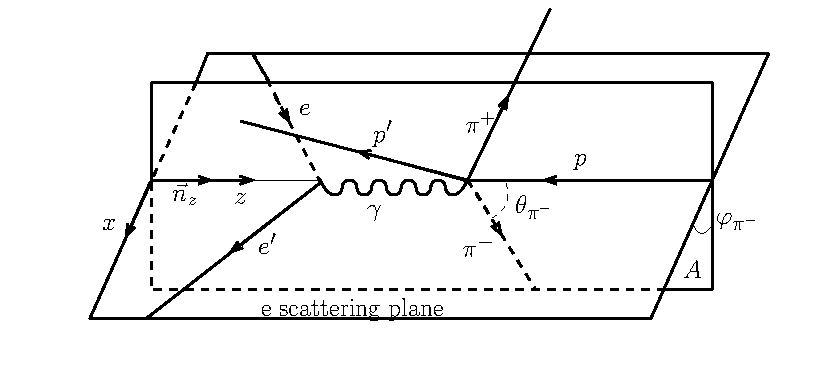
\includegraphics[width=14cm]{pictures/cross_section/thetaphi_new.pdf}
\caption{\small Polar ($\theta_{\pi^{-}}$) and azimuthal ($\varphi_{\pi^{-}}$) angles of the $\pi^{-}$ in the CMS. The $z$-axis is directed along the virtual photon (with the unit vector $\vec n_{z}$), while the $x$-axis is located in the electron scattering plane and follows the direction of the scattered electron. The plane $A$ is defined by the three-momenta of the $\pi^{-}$ and initial proton. } \label{fig:cr_sec_thetaphi}
\end{center}
\end{figure}
\begin{figure}[htp]
\begin{center}
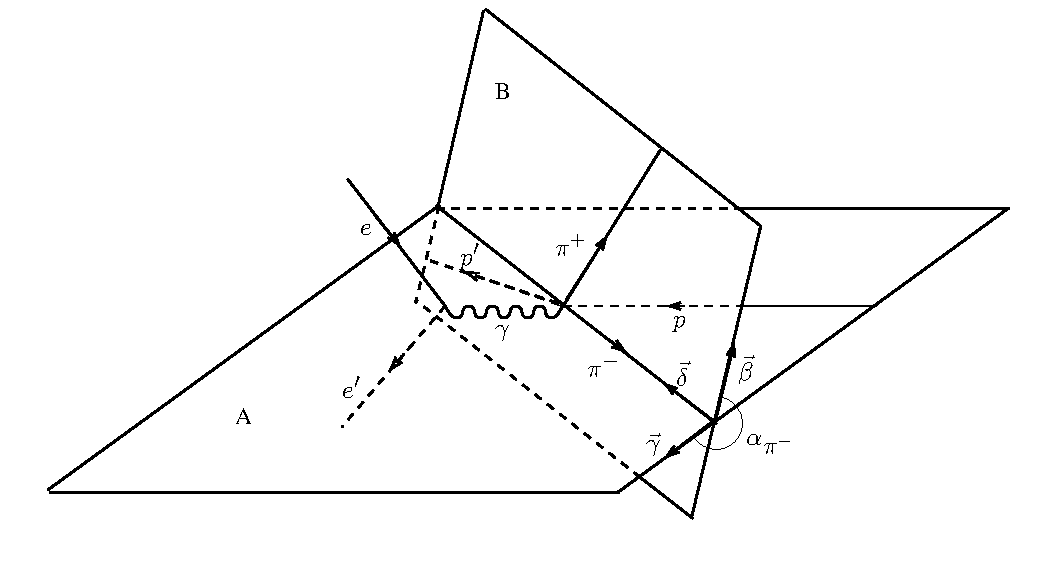
\includegraphics[width=14cm]{pictures/cross_section/alpha1.pdf}
\caption{\small Definition of the angle $\alpha_{\pi^{-}}$ between the two planes: the plane A is defined by  the three-momenta of the $\pi^{-}$ and initial proton, while the plane B is defined by the three-momenta of all final hadrons. The definitions of  auxiliary vectors $\vec \beta$, $\vec \gamma$, and $\vec \delta$ are given in the text.} \label{fig:cr_sec_kinematic2}
\end{center}
\end{figure}



The auxiliary unit vector $\vec \gamma$ is situated in the plane A. This vector is perpendicular to the three-momentum of the $\pi^{-}$ and directed toward the vector $[-\vec n_{z}]$, where $\vec n_{z}$ is the unit vector directed along the $z$-axis. The vector $\vec \gamma$ can be expressed as

\begin{gather*}
\vec \gamma = a_{\alpha}\cdot[-\vec n_{z}]~+~b_{\alpha}\cdot\vec n_{\pi^{-}}  \nonumber \\[10pt]
\text{with~~~}a_{\alpha}  =\sqrt{\frac{1}{1 - (\vec n_{\pi^{-}} \cdot [-\vec n_{z}] )^{2}}}  \text{~~~and~~~} \label{alphavec}
b_{\alpha}  = -  a_{\alpha}\cdot \left (\vec n_{\pi^{-}} \cdot [-\vec n_{z}] \right) \textrm{ ,} \nonumber
\end{gather*}
where $\vec n_{\pi^{-}}$ is the unit vector directed along the three-momentum of the $\pi^{-}$. 



The auxiliary unit vector $\vec \beta$ is situated in the plane B. This vector is perpendicular to the three-momentum of the $\pi^{-}$ and directed toward the three-momentum of the $\pi^{+}$. The vector $\vec \beta$ can be expressed as
\begin{gather*}
\vec \beta = a_{\beta}\cdot\vec n_{\pi^{+}}~+~b_{\beta}\cdot\vec n_{\pi^{-}}  \nonumber \\[10pt]  
\text{with~~~}a_{\beta} = \sqrt{\frac{1}{1 - (\vec n_{\pi^{+}} \cdot \vec n_{\pi^{-}})^{2}}} \text{~~~and~~~} \label{betavec}
b_{\beta} = -  a_{\beta}\cdot(\vec n_{\pi^{+}} \cdot \vec n_{\pi^{-}}) \textrm{ ,} \nonumber
\end{gather*} 
where $\vec n_{\pi^{+}}$ is the unit vector directed along the three-momentum of the $\pi^{+}$. 

Taking the scalar products $(\vec \gamma \cdot \vec  \gamma)$, $(\vec \beta \cdot \vec  \beta)$, $(\vec \gamma \cdot \vec n_{\pi^{-}})$, and $(\vec \beta \cdot \vec n_{\pi^{-}})$, it is straightforward to verify that $\vec \gamma$ and $\vec  \beta$ are the unit vectors perpendicular to the three-momentum of the $\pi^{-}$.

The auxiliary unit vector $\vec \delta$ is the vector product of the auxiliary vectors $\vec \gamma$ and $\vec \beta$, i.e. 
\begin{equation}
\vec \delta = [ \vec \gamma \times \vec \beta ].
\end{equation}

Then the angle $\alpha_{\pi^{-}}$ is determined as:
\begin{equation}
\begin{aligned}
\alpha_{\pi^{-}} &= \arccos(\vec \gamma \cdot \vec \beta),&\text{~~if~~~} \vec \delta~\uparrow\uparrow~\vec n_{\pi^{-}},\\
\alpha_{\pi^{-}} &= 2\pi - \arccos(\vec \gamma \cdot \vec \beta),&\text{~~if~~~} \vec \delta~\uparrow\downarrow~\vec n_{\pi^{-}}.    \label{eq:cr_sec_anglealpha}
\end{aligned}
\end{equation}

The kinematic variables for the first and third sets are calculated in a similar way. The angles $\alpha_{p'}$ and $\alpha_{\pi^{+}}$ are shown for the convenience in Figs.~\ref{fig:cr_sec_kinematic1} and ~\ref{fig:cr_sec_kinematic3}. Further information on the kinematic of reactions with multi-particle final states can be found in Ref.~\cite{Byckling:1971vca}.


%\clearpage
\begin{figure}[htp]
\begin{center}
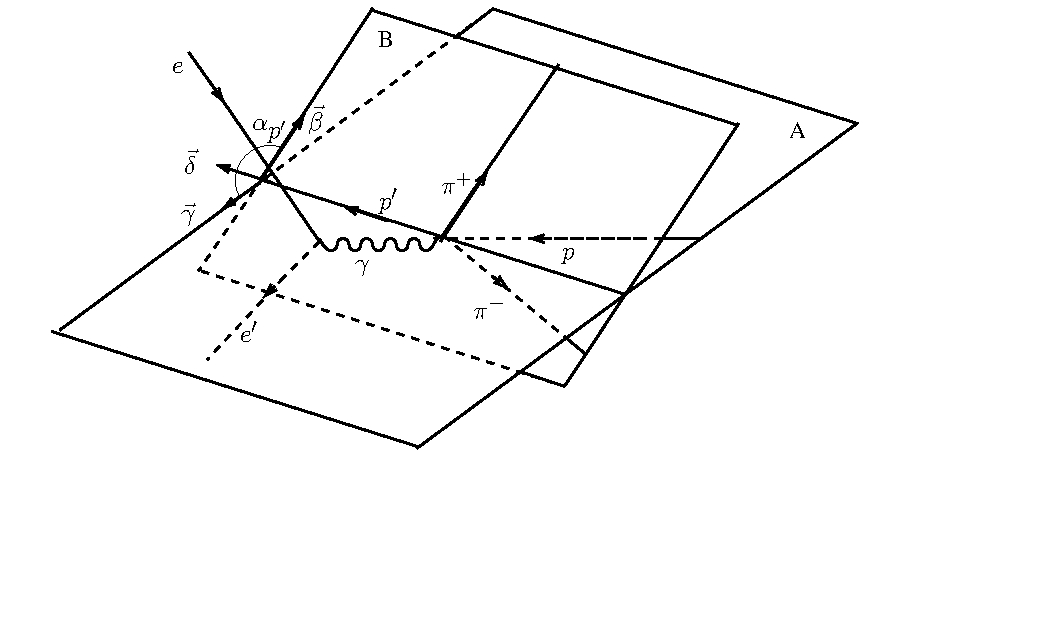
\includegraphics[width=12cm]{pictures/cross_section/alpha2.pdf}
\caption{\small Definition of the angle $\alpha_{p'}$ between the two planes:  the plane A is defined by the three-momenta of initial and scattered protons, while the plane B is defined by the three-momenta of all final hadrons.} \label{fig:cr_sec_kinematic1}
\end{center}
\end{figure}
\begin{figure}[htp]
\begin{center}
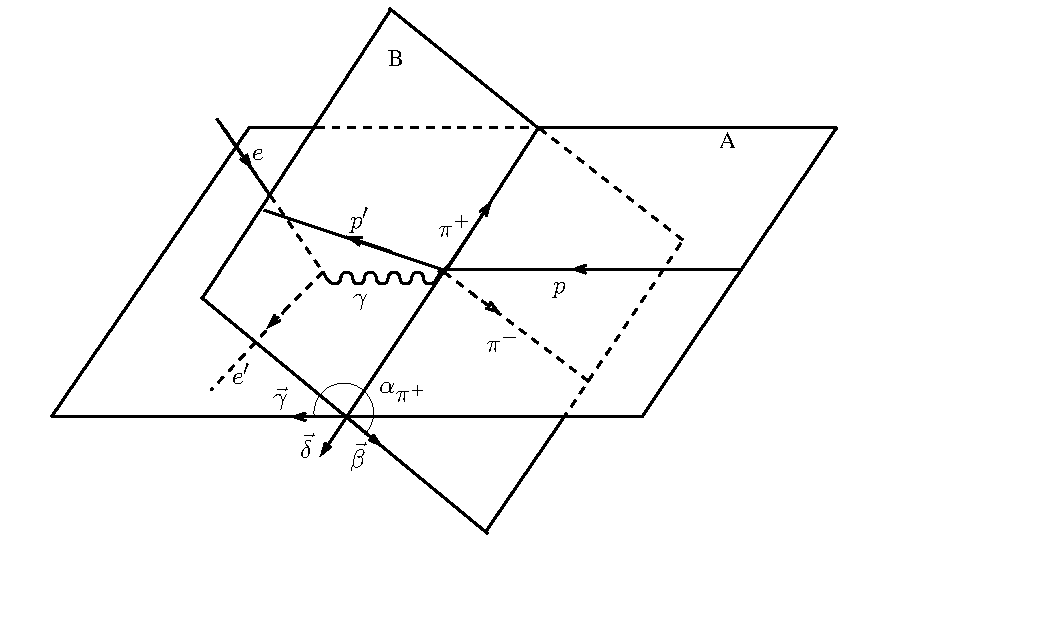
\includegraphics[width=12cm]{pictures/cross_section/alpha3.pdf}
\caption{\small Definition of the angle $\alpha_{\pi^{+}}$ between the two planes: the plane A is defined by the three-momenta of the $\pi^{+}$ and initial proton, while the plane B is defined by the three-momenta of all final hadrons.} \label{fig:cr_sec_kinematic3}
\end{center}
\end{figure}
\clearpage



\section{Binning and kinematic coverage}
\label{Sect:binning}

The available kinematic coverage in the initial state variables is shown by the $Q^2$ versus $W$ distribution\footnote[7]{Note that $W$ here is $W_{sm}$, and therefore, the distribution boundaries are not subject to the blurring. See Sect.~\ref{Sect:smearing_blurring} for details.} in Fig.~\ref{fig:q2_vs_w}. This distribution is filled with the double-pion events survived after the event selection described above. The blue boundary limits the analyzed kinematic area, where the double-pion cross sections are extracted. The black grid demonstrates the chosen binning in the initial state variables (25~MeV in $W$ and 0.05~GeV$^{2}$ in $Q^{2}$).



\begin{figure}[htp]
\begin{center}
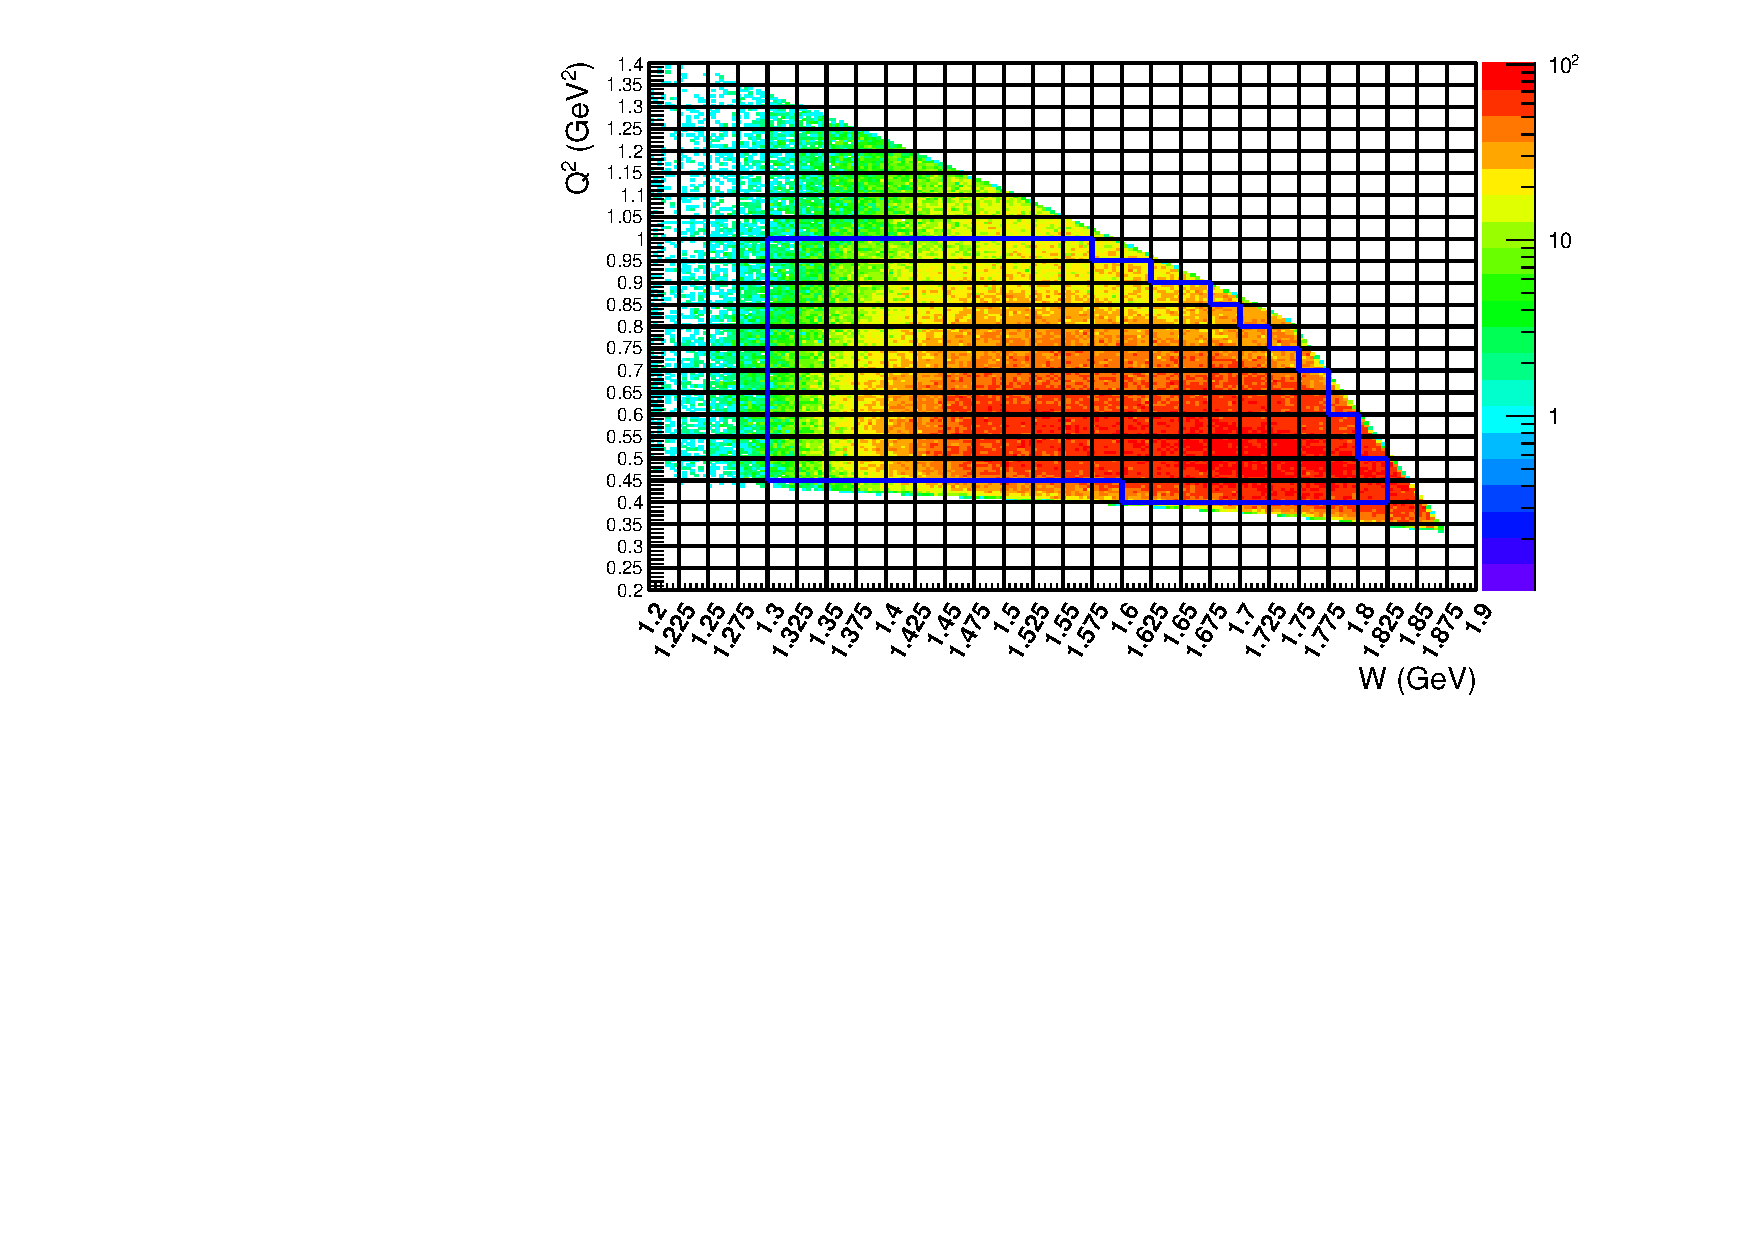
\includegraphics[width=0.95\textwidth]{pictures/cross_section/q2vsw_new.pdf}
\caption{\small $Q^2$ versus $W$ distribution$^{7}$ populated with the selected double-pion events. The cross section is calculated in 2D cells within the blue boundaries.} \label{fig:q2_vs_w}
\end{center}
\end{figure}

The kinematic coverage in the final state variables has the following reaction related features. The angular variables $\theta_{h_{1}}$, $\varphi_{h_{1}}$, and $\alpha_{h_{1}}$ vary in the fixed ranges of $[0,~\pi]$, $[0,~2\pi]$, and $[0,~2\pi]$, respectively. Meanwhile, the ranges of the invariant masses $M_{h_{1}h_{2}}$ and $M_{h_{2}h_{3}}$ are $W$ dependent and broaden as $W$ grows. More details on the specificity of the double-pion production phase-space are given in App.~\ref{app_ph_space}. 

The binning in the final hadron variables used in this study is listed in Tab.~\ref{tab:summary_bins}. In each $W$ and $Q^{2}$ bin the range of each final hadron variable is divided into bins of equal size. However, the number of bins differs in various $W$ subranges, in order to take into account (i) the statistics drop near the reaction threshold, which is at $\approx$~1.22~GeV and (ii) the aforementioned broadening of the reaction phase-space with increasing $W$. The chosen amount of bins in each considered $W$ subrange reflects the intention to maintain reasonable statistical uncertainties of the single-differential cross sections for all $W$ and $Q^2$ bins. 

% The binning choice also takes into account the cross section drop near the double-pion production threshold at $\approx$ 1.22 GeV as well as the broadening of the reaction phase-space with increasing $W$ (see more details in App.~\ref{app_ph_space}).
%\footnote[8]{See more details on the shape of the reaction phase-space in invariant masses in App.~\ref{app_ph_space}.}.

%\begin{table}[htp]
%\centering 
%\caption{\small Number of bins for the given final hadron variables. \label{tab:summary_bins}}
%\begin{tabular}{|c|C{0.13\textwidth}|C{0.13\textwidth}|C{0.15\textwidth}|C{0.18\textwidth}|}
%\hline \multirow{2}{*}{\diagbox[width=3cm, height=2.3cm]{\raisebox{7pt}{$W$ range}}{\raisebox{-10pt}{Variable}}} &Number of bins in invariant mass $M$ &Number of  bins in polar angle $\theta$ &Number of bins in  azimuthal angle $\varphi$ &Number of bins in angle between two planes $\alpha$ \\
%\hline
% 1.3 - 1.35 GeV & 8 & 6 & 5 & 5\\
%\hline
%1.35 - 1.4 GeV & 10 & 8 & 5 & 6\\
%\hline 
% 1.4 - 1.45 GeV & 12 & 10 & 5 & 8\\
%\hline 
% $ > 1.45$ GeV & 12 & 10 & 8 & 8\\
%\hline 
%\end{tabular}
%\end{table}

For the binning in the polar angle note the following. The cross section, although being differential in $[-\cos\theta]$, is binned in $\theta$. These $\Delta \theta$ bins are of equal size in the corresponding $W$ subrange. See also Sect.~\ref{Sect:cr_sect_formula} on this matter.


%. This increases the number of bins filled with event, which and hence from 80\% to 100\% (as $W$ decreases) of bins turn out to be filled with events and involved in the cross section calculation.   
\vspace{0.5em}
\begin{table}[htb]
\centering 
  \caption{Number of bins for hadronic variables.} \label{tab:summary_bins}
  \begin{tabular}{lm{4cm}cccc}
    \toprule
    & & \multicolumn{4}{c}{W subrange (GeV)} \\
    \multicolumn{2}{c}{\centering Hadronic variable }  & [1.3,~1.35] & [1.35,~1.4] & [1.4,~1.475] & [1.475,~1.825] \\
    \cmidrule(l{5pt}r{15pt}){1-2} \cmidrule(l{5pt}r{5pt}){3-6}
    $M_{h_{1}h_{2}}$   & Invariant mass       &   8  & 10 & 12 & 12  \\
    $M_{h_{2}h_{3}}$   & Invariant mass       &   8  & 10 & 12 & 12  \\
    $\theta_{h_{1}}$   & Polar angle          &   6  & 8  & 10 & 10  \\
    $\varphi_{h_{1}}$  & Azimuthal angle      &   5  & 5  & 5  & 6   \\
    $\alpha_{h_{1}}$   & Angle between planes &   5  & 6  & 8  & 8   \\
    \cmidrule(l{5pt}r{15pt}){1-2} \cmidrule(l{5pt}r{5pt}){3-6}
              & Total number of bins \newline in hadronic variables &   9600  & 24000  & 57600  & 69120   \\
    \bottomrule
  \end{tabular}
\end{table}
\vspace{0.5em}

The total numbers of multi-dimensional bins for the corresponding $W$ ranges are listed in the last row of Tab.~\ref{tab:summary_bins} and require some clarification. In fact the invariant masses border of the double-pion production phase-space is $W$-dependent and determined by the Byckling function (see App.~\ref{app_ph_space}). Therefore, the bins located outside this border contain no double-pion events and hence do not contribute to the cross section. For a given $W$ value, the border is distinct, however for a $W$ bin, which corresponds to a range of $W$ values, it is somewhat diffused. If events are binned in $W_{true}$ (like in a free proton experiment) and the bin is small, e.g. 25 MeV, this diffusion is marginal. Then the quantity of bins involved in the cross section calculation (including both non-empty and empty cells) varies from 90\% to 70\% of the total numbers given in the last row of Tab.~\ref{tab:summary_bins} as $W$ increases from the threshold. However, if events are binned in $W_{sm}$ (like in this analysis), each $W_{sm}$ value in a bin corresponds to a sequence of $W_{true}$ spread over 50-100 MeV. In this case a very pronounced boundary diffusion takes place, increasing the quantity of bins filled with events, i.e. the fraction of bins involved in the cross section calculation turn out to vary from 100\% to 80\% as $W$ increases\footnote[8]{This estimation is based on the Monte Carlo simulation performed with TWOPEG~\cite{twopeg} and TWOPEG-D~\cite{twopeg-d} for the reactions off the proton at rest and off the moving proton, respectively.}.


%\footnote[7]{Note that the actual number of bins involved in the cross section calculation is slightly less (by $<$1\%) due to the restrictions imposed by the Byckling function on the double-pion production phase-space.}

%Since the border of the double-pion production phase in invariant masses is determined by the Byckling function, the actual number of bins filled with the double-pion events is less than the number listed in the table. If events are binned in $W_{true}$ (like in the free proton experiment) the number of filled bins is 80\%-90\% of the listed in the table. However, the necessity to bin events in $W_{sm}$ (like in this analysis) leads to the fact that each $W$ bin contain the mixture of events with different $W_{true}$ and as a result -- with different size of the phase-space in invariant masses. The overlap of different 

The specific organization of the double-pion production phase-space in the invariant masses $(M_{h_{1}h_{2}}, M_{h_{2}h_{3}})$ causes the need to pay special attention to the binning in these variables. Equation~\eqref{eq:inv_mass_boundary} gives the expressions for the lower and upper boundaries of the $M_{h_{1}h_{2}}$ distribution and demonstrates that the upper boundary depends on the value of $W$, while the lower does not (see also App.~\ref{app_ph_space} on this matter).
\begin{equation}
\begin{aligned}
M_{lower} &= m_{h_1} + m_{h_2} \\
M_{upper} (W) &= W - m_{h_3}. \label{eq:inv_mass_boundary}
\end{aligned}  
\end{equation}

Here $m_{h_1}$, $m_{h_2}$, and $m_{h_3}$ are the masses of the final hadrons. 


Since the cross section is calculated in a bin $W_{left} < W < W_{right}$, the boundary of $M_{upper}$ is not distinct. For the purpose of binning in mass, the value of $M_{upper}$ is calculated using $W_{center}$, at the center of the $W$ bin. As a result, some events with $W > W_{center}$ turned out to be located beyond $M_{upper}$. Hence it was decided to use a specific arrangement of mass bins with the bin width $\Delta M$ determined by
\begin{equation}
\begin{aligned}
\Delta M = \frac{M_{upper}-M_{lower}}{N_{bins}-1}, \label{eq:bin_width}
\end{aligned}  
\end{equation} 
where $N_{bins}$ is the number of bins specified in the first row of Tab.~\ref{tab:summary_bins}. The left boundary of the first bin is set to $M_{lower}$.

The chosen arrangement of bins forces the last bin to be situated completely out of the boundaries given by Eq.~\eqref{eq:inv_mass_boundary} using $W_{center}$\footnote[9]{Note that for each $W$ bin and for each invariant mass, $\Delta M$ given by Eq.~\eqref{eq:bin_width} is greater than 12.5~MeV, which is the half of the $W$ bin width.}. Therefore, the cross section in this extra bin finally is not reported. However, this bin is kept in the analysis since its content (though being very small) contributes to all cross sections that are obtained by integrating over the corresponding invariant mass distribution. 

% Although the cross section obtained in this extra bin is very small, it is kept in the analysis since its content contributes to all cross sections that are obtained by integrating over the corresponding invariant mass distribution. Other than that, however, the cross section in this extra bin is not considered and finally not reported.

Note that the cross section in the next to last bin in invariant mass needs a special correction. This correction is described in Sect.~\ref{Sect:bin_cor}.



%===============================================

\section{Cross section formulae}
\label{Sect:cr_sect_formula}

\subsection{Electron scattering cross section}

The experimental electron scattering cross section $\sigma_{e}$ for the reaction $ep(n) \rightarrow e'p'(n') \pi^{+} \pi^{-}$ is seven-fold differential and calculated as\footnote[10]{To deal with the multi-differential cross section, THnSparse multi-dimensional root histograms are used.}
\begin{equation}
\frac{\textrm{d}^{7}\sigma_{e}}{\textrm{d}W\textrm{d}Q^{2}\textrm{d}^{5}\tau} = \frac{1}{ R \! \cdot \! \mathcal{F}}  \cdot 
\frac{\left( \frac{N_{full}}{Q_{full}}-\frac{N_{empty}}{Q_{empty}} \right)}{
\Delta W \! \cdot \! \Delta Q^{2} \! \cdot \! \Delta^{5} \tau \! \cdot \! \left[ \frac{l \cdot \rho \cdot N_{A}}{q_{e}\cdot \mu_{d}} \right]\! \cdot \!\mathcal{E}} \textrm{ , where}
\label{expcrossect}
\end{equation}
%where
%\vspace{-2.4em}
\begin{itemize}
\item $\textrm{d}^{5}\tau = \textrm{d}M_{h_{1}h_{2}} \textrm{d}M_{h_{2}h_{3}} \textrm{d}\Omega_{h_1} \textrm{d}\alpha_{h_1}$ is the differential of the five independent variables of the $\pi^{+}\pi^{-}p$ final state, which are described in Sect.~\ref{Sect:kin_var};\vspace{-0.25em}
\item $N_{full}$ and $N_{empty}$ are the numbers of selected double-pion events inside the seven-dimensional bin for runs with deuterium and empty target, respectively;\vspace{-0.25em} %Each event was weighted with the corresponding photoelectron correction factor given by Eq.~\eqref{eq:cc_corr_fact}.\vspace{-0.25em}
\item the quantity in the square brackets in the denominator corresponds to the luminosity of the experiment $\mathcal{L}$ in the units cm$^{-2}\cdot$C$^{-1}$ and its components are\vspace{-0.25em}
\begin{itemize}
\item [ ]  $l$ = 2 cm the length of the target,\vspace{-0.4em}
\item [ ]  $\rho$ = 0.169 g$\cdot$cm$^{-3}$ the density of liquid deuterium,\vspace{-0.4em}
\item [ ]  $N_{A}$ = 6.022$\cdot 10^{-19}$ mol$^{-1}$ Avogadro's number,\vspace{-0.4em}
\item [ ]  $q_{e}$ = 1.602$\cdot 10^{-19}$ C the elementary charge, and \vspace{-0.4em}
\item [ ]  $\mu_{d}$ = 2.014 g$\cdot$mol$^{-1}$ the molar mass of deuterium,\vspace{-0.25em}
\end{itemize}
which results in the luminosity value of $\mathcal{L}$ = 0.63$\cdot$10$^{42}$ cm$^{-2}\cdot$C$^{-1}$ = 0.63$\cdot$10$^{12}$ $\mu$b$^{-1}\cdot$C$^{-1}$;\vspace{-0.25em}


\item $Q_{full}$ = 3734.69 $\mu C$ and $Q_{empty}$ = 464.797 $\mu C$ are the values of the charge accumulated in the Faraday Cup for deuterium and empty target runs, respectively\footnote[11]{They are calculated by summing up the charges of all analyzed \textit{blocks} (see Sect.~\ref{Sect:qcheck} for details).}, which results in the corresponding values of the integrated luminosity $L=\mathcal{L}\cdot Q$ of 2.35$\cdot 10^{9}$ $\mu \text{b}^{-1}$ and 0.29$\cdot 10^{9}$ $\mu \text{b}^{-1}$; \vspace{-0.25em}

\item $\mathcal{E} = \mathcal{E}(\Delta W, \Delta Q^{2}, \Delta^{5}\tau)$ is the detector efficiency (which includes the detector acceptance) for each seven-dimensional bin as determined by the Monte Carlo simulation (see Sect.~\ref{Sect:eff_eval}); \vspace{-0.25em}

\item $R = R(\Delta W, \Delta Q^{2})$ is the radiative correction factor described in Sec.~\ref{Sect:rad_corr}; \vspace{-0.25em}

\item $\mathcal{F} = \mathcal{F}(\Delta W, \Delta Q^{2}, \Delta^{5}\tau)$ is the correction factor that aims at unfolding the effects of the target motion (see Sect.~\ref{Sect:fermi_corr}).

\end{itemize}

The electron scattering cross section $\sigma_{e}$ in the left hand side of Eq.~\eqref{expcrossect} is assumed to be obtained in the center of the finite seven-dimensional kinematic bin $\Delta W \Delta Q^{2} \Delta^{5} \tau$. 





\subsection{Virtual photoproduction cross section}

The goal of the analysis is to extract the virtual photoproduction cross section $\sigma_{v}$ of the reaction $\gamma_{v}p(n) \rightarrow p'(n') \pi^{+} \pi^{-}$. This virtual photoproduction cross section $\sigma_{v}$ is five-fold differential and in the single-photon exchange approximation connected with the seven-fold differential electron scattering cross section\footnote[12]{Note that after the corrections introduced in Eq.~\eqref{expcrossect} by the factors $R$ and $\mathcal{F}$, the cross section $\sigma_{e}$ is the true electron scattering cross section attributed to the central values of the corresponding $\Delta W \Delta Q^{2} \Delta^{5} \tau$ bin and the distinct value of the beam energy $E_{beam} = 2.039$~GeV.} $\sigma_{e}$ via 
\begin{equation}
\begin{aligned}
\frac{\textrm{d}^{5}\sigma_{v}}{\textrm{d}^{5}\tau} &= \frac{1}{\Gamma_{v}}\frac{\textrm{d}^{7}\sigma_{e}}{\textrm{d}W\textrm{d}Q^{2}\textrm{d}^{5}\tau}  \textrm{ ,}
\end{aligned} 
\label{fulldiff}
\end{equation}
where $\Gamma_{v}$ is the virtual photon flux given by
\begin{equation}
\Gamma_{v} (W, Q^2) =
\frac{\alpha}{4\pi}\frac{1}{E_{beam}^{2}m_{p}^{2}}\frac{W(W^{2}-m_{p}^{2})}
{(1-\varepsilon_{T})Q^{2}} \textrm{ .}
\label{flux}
\end{equation}

Here $\alpha$ is the fine structure constant $\left(1/137\right)$, $m_{p}$ the proton mass, $E_{beam}$ = 2.039 GeV the laboratory energy of the incoming electron beam, and $\varepsilon_{T}$ the virtual photon transverse polarization given by \vspace{-1em}
\begin{equation}
\varepsilon_{T} = \left( 1 + 2\left( 1 +
\frac{\nu^{2}}{Q^{2}} \right)
\tan^{2}\left(\frac{\theta_{e'}}{2}\right) \right)^{-1} \textrm{ ,}
\label{polarization}
\end{equation}
where $\nu = E_{beam} - E_{e'}$ is the virtual photon energy, while $E_{e'}$ and $\theta_{e'}$ are the energy and the polar angle of the scattered electron in the lab frame, respectively. 
%$W$, $Q^{2}$ and $\theta_{e'}$ are taken in the center of the bin.

The value of the virtual photon flux given by Eq.~\eqref{flux} is calculated for the central point of the $\Delta W \Delta Q^{2}$ bin. %Note that the $\Gamma_{v}$ is calculated using the smeared value of $W$. A correction for this approximation is included into the procedure of unfolding the effects of the target motion (see Sect.~\ref{Sect:fermi_corr}). Therefore, $\sigma_{v}$ in the left hand side of the Eq.~\eqref{fulldiff} is attributed to the non-smeared value of $W$. 

The limited statistics of the experiment does not allow for estimates of the five-fold differential cross section $\sigma_{v}$ with a reasonable accuracy. Therefore, the cross section $\sigma_{v}$ is first obtained on the multi-dimensional grid and then is integrated over at least four hadron variables. Hence, only the sets of the single-differential and fully-integrated cross sections are obtained.


%being obtained on the multi-dimensional grid, the cross section $\sigma_{v}$ is then 

For each $W$ and $Q^{2}$ bin, the following cross sections are extracted for each variable set.
\begin{equation}
\begin{aligned}
\frac{\textrm{d}\sigma_{v}}{\textrm{d}M_{h_{1}h_{2}}} & =\int\frac{\textrm{d}^{5}\sigma_{v}}{\textrm{d}^{5}\tau}\textrm{d}M_{h_{2}h_{3}}\textrm{d}\Omega_{h_{1}}\textrm{d}\alpha_{h_{1}}, \\
\frac{\textrm{d}\sigma_{v}}{\textrm{d}M_{h_{2}h_{3}}} & =\int\frac{\textrm{d}^{5}\sigma_{v}}{\textrm{d}^{5}\tau}\textrm{d}M_{h_{1}h_{2}}\textrm{d}\Omega_{h_{1}}\textrm{d}\alpha_{h_{1}}, \\
\frac{\textrm{d}\sigma_{v}}{\textrm{d}[-\cos\theta_{h_{1}}]} & =\int\frac{\textrm{d}^{5}\sigma_{v}}{\textrm{d}^{5}\tau}\textrm{d}M_{h_{1}h_{2}}\textrm{d}M_{h_{2}h_{3}}\textrm{d}\varphi_{h_{1}}d\alpha_{h_{1}}, \\
\frac{\textrm{d}\sigma_{v}}{\textrm{d}\alpha_{h_{1}}} & =\int\frac{\textrm{d}^{5}\sigma_{v}}{\textrm{d}^{5}\tau}\textrm{d}M_{h_{1}h_{2}}\textrm{d}M_{h_{2}h_{3}}\textrm{d}\Omega_{h_{1}},~~\text{and}\\
\sigma_{v}^{int} (W, Q^{2}) &= \int \frac{d^{5}\sigma_{v}}{\textrm{d}^{5}\tau}\textrm{d}M_{h_{1}h_{2}}\textrm{d}M_{h_{2}h_{3}}\textrm{d}\Omega_{h_{1}}\textrm{d}\alpha_{h_{1}}.
\end{aligned}
\label{inegr5diff}
\end{equation}

%!!! Since the cross sections are obtained on the five-dimensional kinematic grid, the integrals in Eqs.~\eqref{inegr5diff} are calculated numerically on that grid. 

As a final result for each $W$ and $Q^{2}$ bin, the integral cross section $\sigma_{v}^{int}$, averaged over the three variable sets, is reported together with the nine single-differential cross sections given in \eqref{eq:reported_sec}, where each column is taken from the corresponding variable set.
\begin{equation}
\begin{aligned}
&~~~~~~\frac{\textrm{\textrm{d}}\sigma_{v}}{\textrm{d}M_{p'\pi^{+}}}&&~~~~~~\frac{\textrm{d}\sigma_{v}}{\textrm{d}M_{\pi^{-}\pi^{+}}}&&~~~~~~\frac{\textrm{d}\sigma_{v}}{\textrm{d}M_{\pi^{-}p'}}\\[8pt] 
&~~\frac{\textrm{d}\sigma_{v}}{\textrm{d}[-\cos\theta_{p'}]}&&~~\frac{\textrm{d}\sigma_{v}}{\textrm{d}[-\cos\theta_{\pi^{-}}]}&&~~\frac{\textrm{d}\sigma_{v}}{\textrm{d}[-\cos\theta_{\pi^{+}}]}\\[8pt] 
&~~~~~~~\frac{\textrm{d}\sigma_{v}}{\textrm{d}\alpha_{p'}}&&~~~~~~~~\frac{\textrm{d}\sigma_{v}}{\textrm{d}\alpha_{\pi^{-}}}&&~~~~~~~\frac{\textrm{d}\sigma_{v}}{\textrm{d}\alpha_{\pi^{+}}}
\end{aligned}
\label{eq:reported_sec}
\end{equation}

Regarding the middle row in \eqref{eq:reported_sec} note the following. Although being differential in $[-\cos\theta]$, the cross sections are calculated in $\Delta \theta$ bins, which are of equal size in the corresponding $W$ subrange (see Sect.~\ref{Sect:binning} for details). This is a conventional way of presenting the $\theta$-distributions in the studies of double-pion cross sections~\cite{Rip_an_note:2002,Ripani:2002ss,Fed_an_note:2007,Fedotov:2008aa,Isupov:2017lnd,Arjun,Fed_an_note:2017,Fed_paper_2018}.
\newpage

\section{Efficiency evaluation}
\label{Sect:eff_eval}


For the Monte Carlo simulation the TWOPEG-D event generator was used~\cite{twopeg-d}. This is the version of TWOPEG (an event generator for double-pion electroproduction off the free proton~\cite{twopeg}), which is able to simulate the effects of the initial proton motion. In this version of the event generator the Fermi motion of the initial proton is generated according to the Bonn potential~\cite{Machleidt:1987hj} and then naturally merged into the specific kinematics of double-pion electroproduction. TWOPEG-D accounts for radiative effects according to the approach described in Refs.~\cite{Mo:1968cg,twopeg}.

The generated events are passed through the standard detector simulation (GSIM, GPP) and reconstruction procedures (recsis) with the majority of parameters kept the same as in the studies~\cite{Fed_an_note:2017,Markov:2014}, which were also devoted to the ``e1e" run period\footnote[13]{See the beginning of Sect.~\ref{Sect:select} and also App.~\ref{app_code} for more details on the simulation/reconstruction procedure and for the information on the corresponding parameters used in this analysis.}.
%The sequence of the Monte Carlo event reconstruction is given in more detail in the beginning of Sect.~\ref{Sect:select}. The information on the scripts used in this analysis is given in App.~\cite{app_code}.
%More details the procedure are given in the beginning of Sect.~\ref{Sect:select}.   and the parameters used in this analysis is given 



In the studies of double-pion production cross section it is especially important to generate enough Monte Carlo statistics in order to saturate each multi-dimensional bin of the reaction phase-space with events (see Tab.~\ref{tab:summary_bins}). Insufficient Monte Carlo statistics leads to an improper efficiency evaluation and an unnecessary rise in the empty cells contribution (see Sect.~\ref{Sect:empt_cells}), thus systematically affecting the accuracy of the extracted cross sections. For this study the total of about 4$\cdot$10$^{10}$ double-pion events were generated in the investigated kinematic region, which is considered adequate.
%Otherwise, the efficiency cannot be determined properly and the extracted cross section will lack accuracy.

The TWOPEG-D event generator performs a weighted event generation~\cite{twopeg}, i.e. all kinematic variables are generated randomly according to the double-pion production phase-space, while each event generated at a particular kinematic point acquires an individual weight, which corresponds to the cross section at this point.  Therefore, the efficiency factor $\mathcal{E}$ from Eq.~\eqref{expcrossect} is calculated in each $\Delta W\Delta Q^2\Delta^{5}\tau$ bin as\vspace{-0.5em}
\begin{equation}
\begin{aligned}
\mathcal{E}(\Delta W, \Delta Q^2, \Delta^{5}\tau) = \frac{\mathbb{N}_{rec}}{\mathbb{N}_{gen}} =  \frac{\sum\limits_{i=1}^{N_{rec}} w_{i}}{\sum\limits_{j=1}^{N_{gen}} w_{j}} ,
\end{aligned}
\label{eq:eff}
\end{equation}
where $N_{gen}$ is the number of generated double-pion events (without any cuts) inside the multi-dimensional bin, $N_{rec}$ is the number of reconstructed double-pion events that survived in the bin after the event selection, while $\mathbb{N}_{gen}$ and  $\mathbb{N}_{rec}$ are the weighted numbers of the corresponding events and $w$ is a weight of an individual event.

The efficiency in some kinematic bins could not be reliably determined due to boundary effects, bin to bin event migration, and limited Monte Carlo statistics. Such cells were excluded from consideration. They can be differentiated from the cells with reliable efficiency by a larger relative efficiency uncertainty $\delta \mathcal{E}/\mathcal{E}$.

% Due to the fact that $N_{gen}$ and $N_{rec}$ in Eq.~\eqref{eq:eff} are not independent, the usual method of partial derivatives is not applicable in order to calculate $\delta \mathcal{E}$.


Meanwhile, the calculation of the efficiency uncertainty $\delta \mathcal{E}$ is not straightforward and needs special attention, since (i) $N_{gen}$ and $N_{rec}$ in Eq.~\eqref{eq:eff} are not independent and (ii) Monte Carlo events in this equation are subject to weighting. Therefore, the special approach described in Ref.~\cite{Laforge:1996ts} was used to calculate $\delta \mathcal{E}$. Neglecting the event migration between the bins, this approach gives the following expression for the absolute statistical uncertainty of the efficiency in a bin for the case of weighted Monte Carlo simulation,
\begin{equation}
\begin{aligned}
\delta \mathcal{E} = \sqrt{\frac{\mathbb{N}_{gen} - 2\mathbb{N}_{rec}}{\mathbb{N}_{gen}^{3}}\sum\limits_{i=1}^{N_{rec}} w_{i}^{2} + \frac{\mathbb{N}_{rec}^{2}}{\mathbb{N}_{gen}^{4}}\sum\limits_{j=1}^{N_{gen}} w_{j}^{2}}.
\end{aligned}
\label{eq:eff_err_weighted}
\end{equation}

Meanwhile, according to Ref.~\cite{Laforge:1996ts}, in the case of unweighted Monte Carlo simulation, the formula in Eq.~\eqref{eq:eff_err_weighted} reduces to
\begin{equation}
\begin{aligned}
\delta \widetilde{\mathcal{E}} = \sqrt{\frac{N_{rec}(N_{gen} - N_{rec})}{N_{gen}^{3}}},~\textrm{where}~\widetilde{\mathcal{E}} = \frac{N_{rec}}{N_{gen}}.
\end{aligned}
\label{eq:eff_err_unweighted}
\end{equation}

Figure~\ref{fig:eff_err} (a) shows the distribution of the relative efficiency uncertainty $\delta \mathcal{E}/\mathcal{E}$ versus efficiency $\mathcal{E}$ plotted taking the weights (see Eq.~\eqref{eq:eff_err_weighted}) into account. In this plot the statistical effects turn out to be convoluted with the distribution of weights thus complicating the revealing of cells with unreliable efficiency. To isolate only the statistical effects, the distribution $\delta \widetilde{\mathcal{E}}/\widetilde{\mathcal{E}}$ versus $\widetilde{\mathcal{E}}$, which is produced ignoring the weights (see Eq.~\eqref{eq:eff_err_unweighted}), is plotted in the panel (b). As seen in this plot, the cells with high relative efficiency uncertainty are clustered along the horizontal stripes. This clustering originates from the fact that (if the weights are ignored) the efficiency is obtained by the division of two integer numbers, which reveals the bins with small statistics of the  reconstructed events. These horizontal stripes, furthermore, contain many cells with unreliable extremely small efficiency. Therefore, the following criterion for the selection of cells with reliable efficiency is used $\delta \widetilde{\mathcal{E}}/\widetilde{\mathcal{E}} < 0.3$. This cut is shown in Fig.~\ref{fig:eff_err} (b) by the red horizontal line. All cells above this line were excluded from the analysis. The influence of this cut on the distribution $\delta \mathcal{E}/\mathcal{E}$ (with the weights taken into account) is shown in Fig.~\ref{fig:eff_err} (c).


\begin{figure}[htp]
\begin{center}
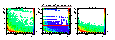
\includegraphics[width=\textwidth]{pictures/cross_section/eff_err/eff_err_16375.pdf}
\caption{\small Distributions of the relative efficiency uncertainty versus efficiency (a) taking into account the weights (see Eq.~\eqref{eq:eff_err_weighted}) and (b) ignoring them (see Eq.~\eqref{eq:eff_err_unweighted}). The cut that aims to select the cells with reliable efficiency is shown by the red horizontal line in panel (b).  Panel (c) shows the influence of this cut on the distribution $\delta \mathcal{E}/\mathcal{E}$ (with the weights taken into account). The distributions are provided for one particular $\Delta W \Delta Q^2$ bin (with the central values specified in figure), and the color code represents the number of multi-dimensional cells within this bin. Note that the $z$-axis maximum for the plot (a) is set the same as for the plot (c).} \label{fig:eff_err}
\end{center}
\end{figure}


The number of reconstructed events in the revealed cells with unreliable efficiency is set to zero ($N_{rec} = 0$). Then such a cell is ranked as an ``empty cell" and, along with other empty cells, is subject to the filling procedure, which is described in Sect.~\ref{Sect:empt_cells}. 


The described above cut on the relative efficiency uncertainty directly impacts the cross section's uncertainties. On the one hand, it eliminates the $\Delta^{5} \tau$ bins with high relative efficiency uncertainty, thus reducing the total statistical uncertainty of the extracted cross sections (see Sect.~\ref{Sect:stat_uncert}). On the other hand, this cut increases the amount of empty cells, thus increasing the cross section's model dependence and the uncertainty associated with it (see Sect.~\ref{Sect:mod_dep}). The cut value is therefore chosen as a compromise between these two effects. 


The idea of this cut is taken from the study~\cite{Fed_an_note:2017,Fed_paper_2018}, which uses unweighted Monte Carlo simulation and therefore employs Eq.~\eqref{eq:eff_err_unweighted} to calculate the efficiency uncertainty. The study~\cite{Fed_an_note:2017,Fed_paper_2018} observed the similar cell clustering along horizontal stripes as that revealed in this analysis in the distributions of $\delta \widetilde{\mathcal{E}}/\widetilde{\mathcal{E}}$ versus $\widetilde{\mathcal{E}}$ (produced ignoring the weights) and also set the cut at the position of 0.3. 
%Therefore, in this analysis the cut position is chosen to be the same as in the study~\cite{Fed_an_note:2017,Fed_paper_2018} (i.e. at 0.3).


Note that in this particular analysis the formula~\eqref{eq:eff_err_unweighted} for the unweighted Monte Carlo is used only for selecting the bins with reliable efficiency, since it allows the pure statistical behavior of the efficiency uncertainty to be determined. For the estimation of the cross section's statistical uncertainty the weights are taken into account and the formula~\eqref{eq:eff_err_weighted} is applied (see Sect.~\ref{Sect:stat_uncert}).




 

\chapter{Corrections to the cross sections}
\label{Sect:corr_cr_sect}

This chapter gives the description of the corrections to the extracted cross sections in the order they were applied.


\section{Filling kinematic cells with zero acceptance}
\label{Sect:empt_cells}

Due to blind areas in the geometrical coverage of the CLAS detector, some kinematic bins of the double-pion production phase-space turned out to have zero acceptance. In such bins, which are usually called empty cells, the cross section cannot be experimentally defined. For the studies, which aim at extracting fully-differential cross sections (i.e. single-pion production analyses), this is not a problem of great importance, since the cross section in blind areas is just not reported. However, in the studies of double-pion production, where the limited experimental statistics allows only single-differential cross sections to be extracted, this issue becomes a point of special attention~\cite{Fed_an_note:2007,Fedotov:2008aa,Fed_an_note:2017,Fed_paper_2018,Isupov:2017lnd,Arjun}. The empty cells contribute to the integrals in Eqs.~\eqref{inegr5diff} along with the other kinematic bins. Ignoring the contribution from the empty cells leads to a systematic cross section underestimation and, therefore, some assumptions for the empty cells' content are needed. This situation causes some model dependence of the final result. 


The map of the empty cells is determined using the Monte Carlo simulation. A cell is treated as empty, if it contains generated events ($N_{gen} >$ 0), but does not contain any reconstructed events ($N_{rec}$ = 0). The cells with unreliable efficiencies, revealed based on the cut on the efficiency uncertainty (see Sect.~\ref{Sect:eff_eval}), are also treated as empty. Empty cells should not be confused with the cells that contain both generated and reconstructed events, but do not contain experimental data, i.e. they appear due to the limited experiment duration, which is taken into account via the normalization on the Faraday Cup charge, and therefore, no model assumptions for them are needed. 


It is conventional practice in the studies of the double-pion production to fill the empty cells by means of the Monte Carlo event generator (usually the one that is used to evaluate the efficiency). The studies~\cite{Rip_an_note:2002,Ripani:2002ss,Fed_an_note:2007,Fedotov:2008aa,Isupov:2017lnd,Arjun} used GENEV~\cite{Genev} (the double-pion event generator based on the JM05 reaction model) for this purpose. The empty cells in these studies were filled with the generated events, which were subject to a special scaling procedure in order to match the experimental data in the regular (non-empty) cells. Meanwhile, the study~\cite{Fed_an_note:2017,Fed_paper_2018} used TWOPEG~\cite{twopeg} for the empty cells filling. TWOPEG is the new double-pion event generator, which is based on the JM15 model and up to now provides the best cross section estimation in the kinematic region $W<$ 2~GeV and $Q^2<$ 1.3~GeV$^{2}$. Since TWOPEG is capable of providing the absolute cross section value for a given kinematic point, the study~\cite{Fed_an_note:2017,Fed_paper_2018} used the cross section estimated by TWOPEG as an assumption for the empty cells content. 

In this particular study the empty cells are filled by means of the TWOPEG-D event generator~\cite{twopeg-d}, which is the version of TWOPEG for moving protons.  Although TWOPEG-D is also capable of providing the absolute cross section value, the empty cells in this study were nevertheless filled with the scaled generated events (as in Refs.~\cite{Rip_an_note:2002,Ripani:2002ss,Fed_an_note:2007,Fedotov:2008aa,Isupov:2017lnd,Arjun}). This method was chosen because TWOPEG-D assumes all events to be produced in the quasi-free regime (ignoring FSI) and therefore somewhat overestimates the quasi-free cross section.


Thus, in this study empty multi-dimensional cells are filled with the Monte Carlo events generated by TWOPEG-D (following Refs.~\cite{Rip_an_note:2002,Ripani:2002ss,Fed_an_note:2007,Fedotov:2008aa,Isupov:2017lnd,Arjun}), relying on the cross section shape implemented in the generator. These generated events are subject to the scaling, which leaving the shape unchanged adjusts the empty cells content to the experimental yield in the regular (non-empty) cells. The scaling is performed individually in each $\Delta W\Delta Q^2$ bin according to the integral yields of the experimental and simulated events in the non-empty cells within this bin. The number of events $N_{model}$ that is assigned as a content for the empty $\Delta^{5}\tau$ cell located in the corresponding $\Delta W\Delta Q^2$ bin is then estimated as
\begin{equation}
\begin{aligned}
N_{model}(\Delta W,\Delta Q^2,\Delta^{5}\tau) = \frac{\mathcal{N}_{data}^{int}}{\mathcal{N}_{rec}^{int}} \! \cdot \!\mathbb{N}_{gen}(\Delta W,\Delta Q^2,\Delta^{5}\tau),
\end{aligned}\label{n_model}
\end{equation}
where $\mathbb{N}_{gen}$ is the weighted number of generated events in the corresponding multi-dimensional bin, while the fraction represents the integral scaling factor with $\mathcal{N}_{data}^{int}$ and $\mathcal{N}_{rec}^{int}$ being the total number of experimental events (normalized by the FC charge) and the total number of reconstructed events in all non-empty $\Delta^{5}\tau$ bins within the considered $\Delta W\Delta Q^2$ bin, respectively. These quantities are given by
\begin{equation}
\begin{aligned}
\mathcal{N}_{data}^{int}(\Delta W,\Delta Q^2) &= \sum_{\substack{All~\Delta^{5}\tau\\ with~N_{rec}>0}} \!\!\! \left [\frac{N_{full}}{Q_{full}}-\frac{N_{empty}}{Q_{empty}} \right ]~\textrm{,~and}\\[8pt]
\mathcal{N}_{rec}^{int}(\Delta W,\Delta Q^2)  &= \sum_{\substack{All~\Delta^{5}\tau\\ with~N_{rec}>0}} \!\!\!\!\!\! \mathbb{N}_{rec},
\end{aligned}\label{ints}
\end{equation}
where  $\mathbb{N}_{rec}$ is the weighted number of reconstructed events in the corresponding $\Delta^{5}\tau$ bin. 



For each empty $\Delta W\Delta Q^2\Delta^{5}\tau$ bin, the quantity given by Eq.~\eqref{n_model} imitates the yield of experimental events normalized by the FC charge and corrected by the detector efficiency (see Eq.~\eqref{expcrossect}). The cross section in the empty cells is then calculated as
\begin{equation}
\frac{\textrm{d}^{7}\sigma_{e}}{\textrm{d}W\textrm{d}Q^{2}\textrm{d}^{5}\tau} = \frac{N_{model}}{
\Delta W \! \cdot \! \Delta Q^{2} \! \cdot \! \Delta^{5} \tau \! \cdot \! \left [ \mathcal{L} \right ] }\textrm{ ,}
\label{cr_sect_empt}
\end{equation}
with $N_{model}$ given by Eq.~\eqref{n_model}, and all other variables explained after Eq.~\eqref{expcrossect}. Note that the empty cells are filled before applying the correction factors $R$ and $\mathcal{F}$.

% situated in the numerator of Eq.~\eqref{expcrossect}. %To estimate the cross section in the empty bins, the value of efficiency $\overline{\mathcal{E}}(\Delta W,\Delta Q^2)$ averaged over non-empty bins is used. This averaged efficiency is determined individually for each $\Delta W\Delta Q^2$ bin as
%\begin{equation}
%\begin{aligned}
%\overline{\mathcal{E}}(\Delta W,\Delta Q^2) =  \frac{1}{n_{bins}}\sum_{\substack{All~\Delta^{5}\tau\\ with~N_{rec}>0}} \!\!\!\!\!\! \mathcal{E},
%\end{aligned}\label{avrg_eff} 
%\end{equation}
%where $n_{bins}$ is the number of bins with $N_{rec}>0$ and $\mathcal{E}$ is defined by Eq.~\eqref{eq:eff}.

Figure~\ref{fig:empt_corr} introduces the single-differential cross sections given by Eqs.~\eqref{inegr5diff} and \eqref{eq:reported_sec}\footnote[1]{Both Figure~\ref{fig:empt_corr} and Table~\ref{tab:int_empt_cont} are given for the cross sections, which (although being divided by the virtual photon flux) are neither corrected for the radiative effects (see Sect.~\ref{Sect:rad_corr}) nor for the effects of the target motion (see Sect.~\ref{Sect:fermi_corr}). }. The empty squares correspond to the case when the contribution from the empty cells was ignored, and the black circles are for the case when that was taken into account in the way described above. The figure demonstrates a satisfactory small contribution from the empty cells (and therefore a small model dependence of the results). Only the edge points in the $\theta$ distributions (middle row) reveal pronounced empty cell contributions due to the negligible/zero CLAS acceptance in the corresponding directions.

Table~\ref{tab:int_empt_cont} demonstrates the relative empty cell contribution to the integral cross sections for all reported $(W,~Q^2)$-points$^{1}$. Different shades of red correspond to different percentage ranges, i.e. the lightest shade corresponds to the contribution $\leq 20$\%, darker shade -- from 21\% to 30\%, and the darkest one shows the contribution $>30$\%. As seen from the table, for most of the $(W,~Q^2)$-points the contribution from the empty cells is kept on a low level of $\sim$15\%, having a small rise at the low $Q^{2}$ and high $W$ boundaries, which originates from the momentum-dependent restrictions on the minimal and maximal polar angles of the scattered electron, respectively (see Sect.~\ref{Sect:fiduc_neg}). Additionally, the rise of the empty cells contribution for small $W\sim1.3$~GeV is thought to be related to the fact that near the production threshold the hadrons carry small momentum and hence failed to be registered since (i) they are more likely bent to the detector holes, (ii) CLAS is not designed to register hadrons with a momentum less than a certain value (see e.g. Fig.~\ref{fig:hadron_id}), and (iii) the smaller the hadron velocity is, the more energy it loses in materials (Bragg peak). A similar rise of the empty cells contribution near the threshold was also observed in Refs.~\cite{Fed_an_note:2017,Fed_paper_2018,Fed_an_note:2007,Fedotov:2008aa}, which are devoted to the double-pion electroproduction off the free proton.

To account for the model dependence, the approach established for the previous studies of double-pion production cross sections is followed~\cite{Isupov:2017lnd,Fed_an_note:2017,Golovach}, i.e. the part of the single-differential cross section that came from the empty cells is assigned a 50\% relative uncertainty. The corresponding absolute uncertainty $\delta_{\text{model}}$ is then combined with the total statistical uncertainty, as was done in Refs.~\cite{Isupov:2017lnd,Fed_an_note:2017,Golovach} (more details are in Sect.~\ref{Sect:stat_uncert}).


\begin{figure}[htp]
\begin{center}
\framebox{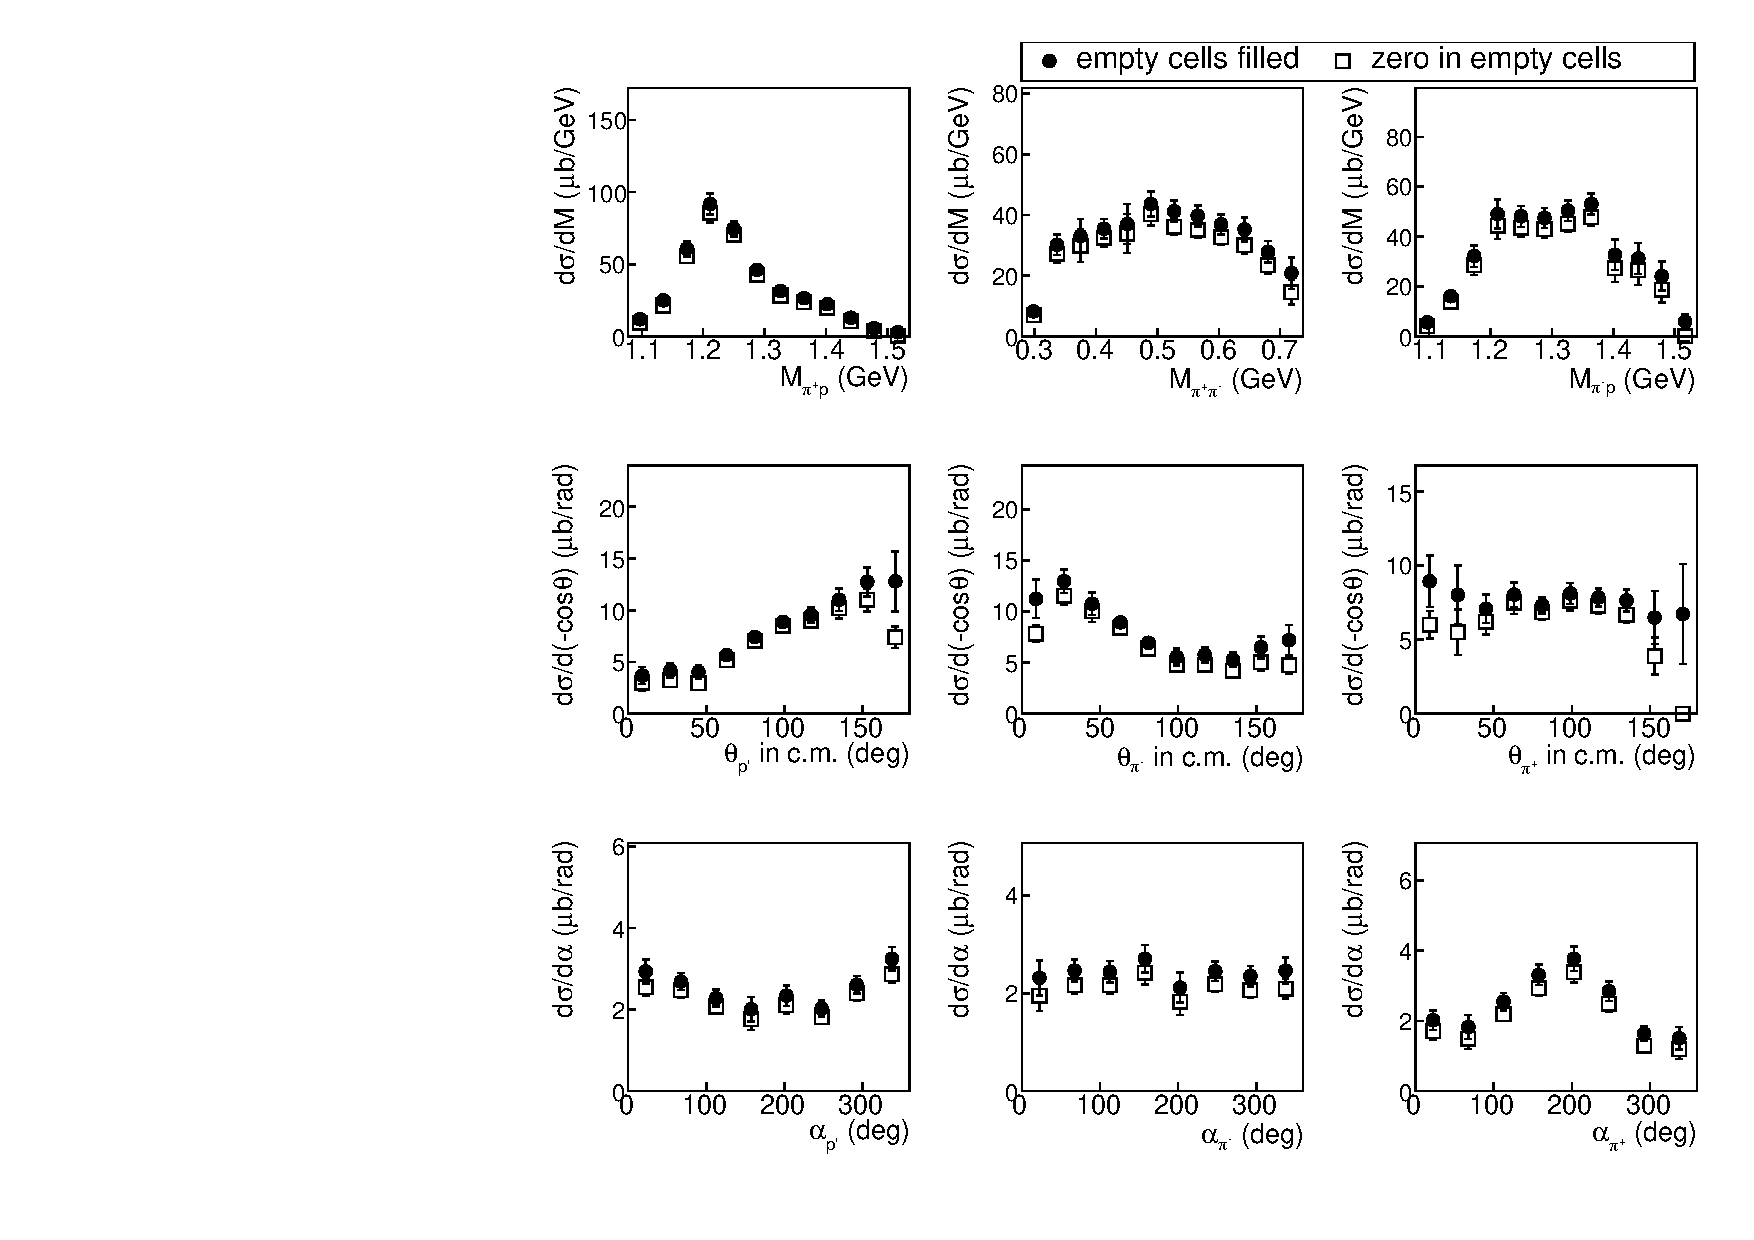
\includegraphics[width=13.75cm]{pictures/corrections/cr_sec_all_top_new.pdf}}
\caption{\small Extracted single-differential cross sections for the cases when the contribution from the empty cells was ignored (empty squares) and when it was taken into account (black circles). The former are reported with the uncertainty $\delta_{\text{stat}}^{\text{tot}}$ given by Eq.~\eqref{errortot}, while the latter are with the uncertainty $\delta_{\text{stat,mod}}^{\text{tot}}$ given by Eq.~\eqref{eq:error_stat_mod}. All distributions are given for one particular bin in $W$ and $Q^2$ ($W = $1.6375 GeV, $Q^2 = $0.625 GeV$^2$).} \label{fig:empt_corr}
\end{center}
\end{figure}


\begin{table}
\begin{center}
\caption{\small Relative empty cell contribution to the integral cross sections for all reported $(W,~Q^2)$-points. The columns correspond to the $Q^2$ values in GeV$^2$ and the rows to the $W$ values in GeV. Different shades of red correspond to different percentage range, i.e. the lightest shade corresponds to the contribution $\leq 20$\%, darker shade -- from 21\% to 30\%, and the darkest one shows the contribution $>30$\%.} \label{tab:int_empt_cont}
\resizebox{\textwidth}{!}{
\begin{tabular}{ ?c?c?c?c?c?c?c?c?c?c?c?c?c? } 
\Xhline{1.5pt}
        &           0.425       &         0.475        &         0.525         &           0.575       &          0.625       & 0.675                &        0.725         &         0.775        &          0.825       &         0.875        &         0.925        & 0.975\\ 
\Xhline{1.5pt}
 1.3125 & {\bf --}	        & \cellcolor{red!60}41 & \cellcolor{red!60}34  &  \cellcolor{red!60}32 & \cellcolor{red!60}35 & \cellcolor{red!60}37 & \cellcolor{red!60}41 & \cellcolor{red!60}33 & \cellcolor{red!60}33 & \cellcolor{red!60}45 & \cellcolor{red!60}35 & \cellcolor{red!60}48 \\ 
\Xhline{1.5pt}
 1.3375 & {\bf --}	        & \cellcolor{red!40}28 & \cellcolor{red!40}28  &  \cellcolor{red!40}27 & \cellcolor{red!40}26 & \cellcolor{red!40}28 & \cellcolor{red!60}31 & \cellcolor{red!60}32 & \cellcolor{red!60}33 & \cellcolor{red!60}35 & \cellcolor{red!60}33 & \cellcolor{red!60}35 \\ 
\Xhline{1.5pt}
 1.3625 & {\bf --} 	        & \cellcolor{red!40}28 & \cellcolor{red!40}26  &  \cellcolor{red!40}23 & \cellcolor{red!40}24 & \cellcolor{red!40}25 & \cellcolor{red!40}25 & \cellcolor{red!40}25 & \cellcolor{red!40}27 & \cellcolor{red!40}27 & \cellcolor{red!40}28 & \cellcolor{red!40}27 \\ 
\Xhline{1.5pt}
 1.3875 & {\bf --} 	        & \cellcolor{red!40}21 & \cellcolor{red!25}19  &  \cellcolor{red!25}18 & \cellcolor{red!25}17 & \cellcolor{red!25}19 & \cellcolor{red!25}19 & \cellcolor{red!25}18 & \cellcolor{red!25}18 & \cellcolor{red!40}21 & \cellcolor{red!40}23 & \cellcolor{red!40}21 \\ 
\Xhline{1.5pt}  
 1.4125 & {\bf --}	        & \cellcolor{red!40}27 & \cellcolor{red!25}20  &  \cellcolor{red!25}18 & \cellcolor{red!25}17 & \cellcolor{red!25}17 & \cellcolor{red!25}18 & \cellcolor{red!25}20 & \cellcolor{red!25}19 & \cellcolor{red!25}20 & \cellcolor{red!25}20 & \cellcolor{red!25}20 \\ 
\Xhline{1.5pt}
 1.4375 & {\bf --}	        & \cellcolor{red!40}23 & \cellcolor{red!25}17  &  \cellcolor{red!25}17 & \cellcolor{red!25}14 & \cellcolor{red!25}14 & \cellcolor{red!25}14 & \cellcolor{red!25}17 & \cellcolor{red!25}15 & \cellcolor{red!25}15 & \cellcolor{red!25}16 & \cellcolor{red!25}18 \\ 
\Xhline{1.5pt}
 1.4625 & {\bf --}	        & \cellcolor{red!40}21 & \cellcolor{red!25}16  &  \cellcolor{red!25}14 & \cellcolor{red!25}13 & \cellcolor{red!25}13 & \cellcolor{red!25}12 & \cellcolor{red!25}13 & \cellcolor{red!25}13 & \cellcolor{red!25}13 & \cellcolor{red!25}14 & \cellcolor{red!25}16 \\ 
\Xhline{1.5pt}
 1.4875 & {\bf --}	        & \cellcolor{red!40}24 & \cellcolor{red!25}18  &  \cellcolor{red!25}15 & \cellcolor{red!25}14 & \cellcolor{red!25}14 & \cellcolor{red!25}13 & \cellcolor{red!25}13 & \cellcolor{red!25}15 & \cellcolor{red!25}15 & \cellcolor{red!25}15 & \cellcolor{red!25}16 \\ 
 \Xhline{1.5pt}
 1.5125 & {\bf --}              & \cellcolor{red!40}23 & \cellcolor{red!25}18  &  \cellcolor{red!25}16 & \cellcolor{red!25}15 & \cellcolor{red!25}14 & \cellcolor{red!25}14 & \cellcolor{red!25}13 & \cellcolor{red!25}14 & \cellcolor{red!25}15 & \cellcolor{red!25}16 & \cellcolor{red!25}16\\ 
\Xhline{1.5pt}
 1.5375 & {\bf --}	        & \cellcolor{red!40}23 & \cellcolor{red!25}19  &  \cellcolor{red!25}16 & \cellcolor{red!25}16 & \cellcolor{red!25}14 & \cellcolor{red!25}14 & \cellcolor{red!25}14 & \cellcolor{red!25}14 & \cellcolor{red!25}17 & \cellcolor{red!25}18 & \cellcolor{red!25}15 \\ 
\Xhline{1.5pt}
 1.5625 & {\bf --}              & \cellcolor{red!40}22 & \cellcolor{red!25}19  &  \cellcolor{red!25}16 & \cellcolor{red!25}16 & \cellcolor{red!25}15 & \cellcolor{red!25}15 & \cellcolor{red!25}15 & \cellcolor{red!25}15 & \cellcolor{red!25}17 & \cellcolor{red!25}17 & \cellcolor{red!25}17 \\ 
\Xhline{1.5pt}
 1.5875 & {\bf --}              & \cellcolor{red!40}23 & \cellcolor{red!25}18  &  \cellcolor{red!25}17 & \cellcolor{red!25}20 & \cellcolor{red!25}15 & \cellcolor{red!25}15 & \cellcolor{red!25}17 & \cellcolor{red!25}16 & \cellcolor{red!25}18 & \cellcolor{red!25}17 & {\bf --}\\ 
\Xhline{1.5pt}
 1.6125 & \cellcolor{red!40}26  & \cellcolor{red!25}20 & \cellcolor{red!25}17  &  \cellcolor{red!25}16 & \cellcolor{red!25}15 & \cellcolor{red!25}15 & \cellcolor{red!25}15 & \cellcolor{red!25}15 & \cellcolor{red!25}17 & \cellcolor{red!25}16 & \cellcolor{red!25}15 & {\bf --}\\ 
 \Xhline{1.5pt}
 1.6375 & \cellcolor{red!40}26  & \cellcolor{red!25}19 & \cellcolor{red!25}17  &  \cellcolor{red!25}16 & \cellcolor{red!25}14 & \cellcolor{red!25}16 & \cellcolor{red!25}14 & \cellcolor{red!25}16 & \cellcolor{red!25}17 & \cellcolor{red!25}16 & {\bf --}             & {\bf --} \\
\Xhline{1.5pt}
 1.6625 & \cellcolor{red!40}25  & \cellcolor{red!25}19 & \cellcolor{red!25}17  &  \cellcolor{red!25}15 & \cellcolor{red!25}15 & \cellcolor{red!25}15 & \cellcolor{red!25}15 & \cellcolor{red!25}17 & \cellcolor{red!25}18 & \cellcolor{red!25}17 & {\bf --}             & {\bf --} \\ 
\Xhline{1.5pt}
 1.6875 & \cellcolor{red!40}24  & \cellcolor{red!25}20 & \cellcolor{red!25}17  &  \cellcolor{red!25}16 & \cellcolor{red!25}15 & \cellcolor{red!25}15 & \cellcolor{red!25}16 & \cellcolor{red!25}19 & \cellcolor{red!25}18 & {\bf --}             & {\bf --}             & {\bf --} \\ 
\Xhline{1.5pt}
 1.7125 & \cellcolor{red!40}23  & \cellcolor{red!25}19 & \cellcolor{red!25}17  &  \cellcolor{red!25}17 & \cellcolor{red!25}16 & \cellcolor{red!25}17 & \cellcolor{red!25}19 & \cellcolor{red!25}18 & {\bf --}             & {\bf --}             & {\bf --}             & {\bf --} \\ 
 \Xhline{1.5pt}
 1.7375 & \cellcolor{red!40}23  & \cellcolor{red!25}20 & \cellcolor{red!25}17  &  \cellcolor{red!25}17 & \cellcolor{red!25}17 & \cellcolor{red!25}18 & \cellcolor{red!25}19 & {\bf --}             & {\bf --}             & {\bf --}             & {\bf --}             & {\bf --} \\
\Xhline{1.5pt}
 1.7625 & \cellcolor{red!40}22  & \cellcolor{red!25}20 & \cellcolor{red!25}18  &  \cellcolor{red!25}18 & \cellcolor{red!25}18 & \cellcolor{red!25}19 & {\bf --}             & {\bf --}             & {\bf --}             & {\bf --}             & {\bf --}             & {\bf --} \\ 
\Xhline{1.5pt}
 1.7875 & \cellcolor{red!40}21  & \cellcolor{red!25}19 & \cellcolor{red!25}18  &  \cellcolor{red!25}18 & {\bf --}             & {\bf --}             & {\bf --}             & {\bf --}             & {\bf --}             & {\bf --}             & {\bf --}             & {\bf --} \\
\Xhline{1.5pt}
 1.8125 & \cellcolor{red!40}21  & \cellcolor{red!25}17 &{\bf --}               &{\bf --}               & {\bf --}             & {\bf --}             & {\bf --}             & {\bf --}             & {\bf --}             & {\bf --}             & {\bf --}             & {\bf --} \\ 
\Xhline{1.5pt}
\end{tabular}}
\end{center}
\end{table}


%\begin{enumerate}

%\item The map of the empty cells is determined using the Monte Carlo simulation. For that purpose, firstly, so-called unit generated histogram and unit reconstructed histogram are obtained as\footnote[4]{All operation with the multi-dimensional histograms given here are implied to be performed with the contents of the corresponding multi-dimensional bins.}

%\begin{equation}
%\begin{aligned}
%&h\_5d\_unit\_gen&=~& h\_5d\_gen/h\_5d\_gen,\\
%&h\_5d\_unit\_rec&=~& h\_5d\_rec/h\_5d\_rec.
%\end{aligned}
%\end{equation}
%These unit histograms have 1 in that bins that were filled and 0 in empty bins.

%Then, the map of the empty cells is obtained as 

%\begin{equation}
%\begin{aligned}
%h\_5d\_map &= h\_5d\_unit\_gen - h\_5d\_unit\_rec.
%\end{aligned}
%\end{equation}

%This unit histogram has 1 in bins where we have generated, but do not have reconstructed, and 0 in other bins.

%\item 

%\end{enumerate}

%F_{data}^{int} = \int [h\_5d\_data/h\_5d\_unit\_rec]\\
%F_{gen}^{int} = \int [h\_5d\_gen/h\_5d\_unit\_rec]\\
%F_{eff}^{avrg} = \frac{1}{N_{bins}} \int [h\_5d\_eff]\\

%\newpage


\section{Radiative correction}
\label{Sect:rad_corr}

The incoming and scattered electrons are subject to radiative effects, which means that they can emit photons thus reducing their energy. However, in the experiment the information on these emissions is not accessible, and one has to assume the electron energy to be unchanged. Therefore, when extracting the cross sections, one assumes the energy of the incoming/scattered electron to be greater/smaller than it actually was in the reaction. This, in turn, leads to the systematic overestimation of the virtual photon energy with the consequent overestimation\footnote[2]{The $Q^2$ value is overestimated if the incoming electron emits and underestimated if the scattered electron emits. That is why the radiative effects do not significantly impact the $Q^{2}$-dependence of the cross section.} of $W$. As a result, the extracted cross section is assigned to the $W$ value higher than the actual one. This distorts the measured $W$ spectrum and leads to its agglomeration in the high-lying region.


The common way of handling this problem is to apply the radiative correction to the extracted cross sections. In this study the radiative correction is performed using TWOPEG-D~\cite{twopeg-d}, which is the event generator for the double-pion electroproduction that simulates effects of the target motion. TWOPEG-D accounts for the radiative effects by means of the well-known approach of Ref.~\cite{Mo:1968cg}, which is traditionally used for the radiative corrections in the studies of double-pion electroproduction~\cite{Rip_an_note:2002,Ripani:2002ss,Fed_an_note:2007,Fedotov:2008aa,Fed_an_note:2017,Fed_paper_2018,Isupov:2017lnd,Arjun}. In Ref.~\cite{Mo:1968cg} the approach is applied to the inclusive case, while in TWOPEG-D, the double-pion integrated cross sections are used instead~\cite{twopeg,twopeg-d}. 

In the approach~\cite{Mo:1968cg,twopeg,twopeg-d} the radiative photons are supposed to be emitted collinearly either to the direction of the incoming or scattered electron (the so-called ``peaking approximation"). The calculation of the radiative cross section is split into two parts. The ``soft" part assumes the energy of the emitted radiative photon to be less than a certain minimal value (10 MeV), while the ``hard" part is for the photons with an energy greater than that value. The ``soft" part is evaluated explicitly, while for the calculation of the ``hard" part, an inclusive hadronic tensor is assumed. The latter assumption is however considered adequate, especially taking into account that approaches that are capable of describing radiative processes in exclusive double-pion electroproduction are not yet available.


The radiative correction factor $R$ in Eq.~\eqref{expcrossect} is determined in the following way. The double-pion events either with or without radiative effects are generated with TWOPEG-D. Both radiated and non-radiated events are subjected to the smearing due to the Fermi motion of the target. Then the ratio given by Eq.~\eqref{eq:rad_corr} is taken in each $\Delta W \Delta Q^{2}$ bin.
\begin{equation}
R(\Delta W, \Delta Q^{2}) = \frac{\mathbb{N}_{rad}}{\mathbb{N}_{norad}},
\label{eq:rad_corr}
\end{equation}
where $\mathbb{N}_{rad}$ and $\mathbb{N}_{norad}$ are the weighted numbers of generated events in each $\Delta W \Delta Q^{2}$ bin with and without radiative effects, respectively. Note that neither $\mathbb{N}_{rad}$ nor $\mathbb{N}_{norad}$ are subject to any cuts.

\begin{figure}[htp]
\begin{center}
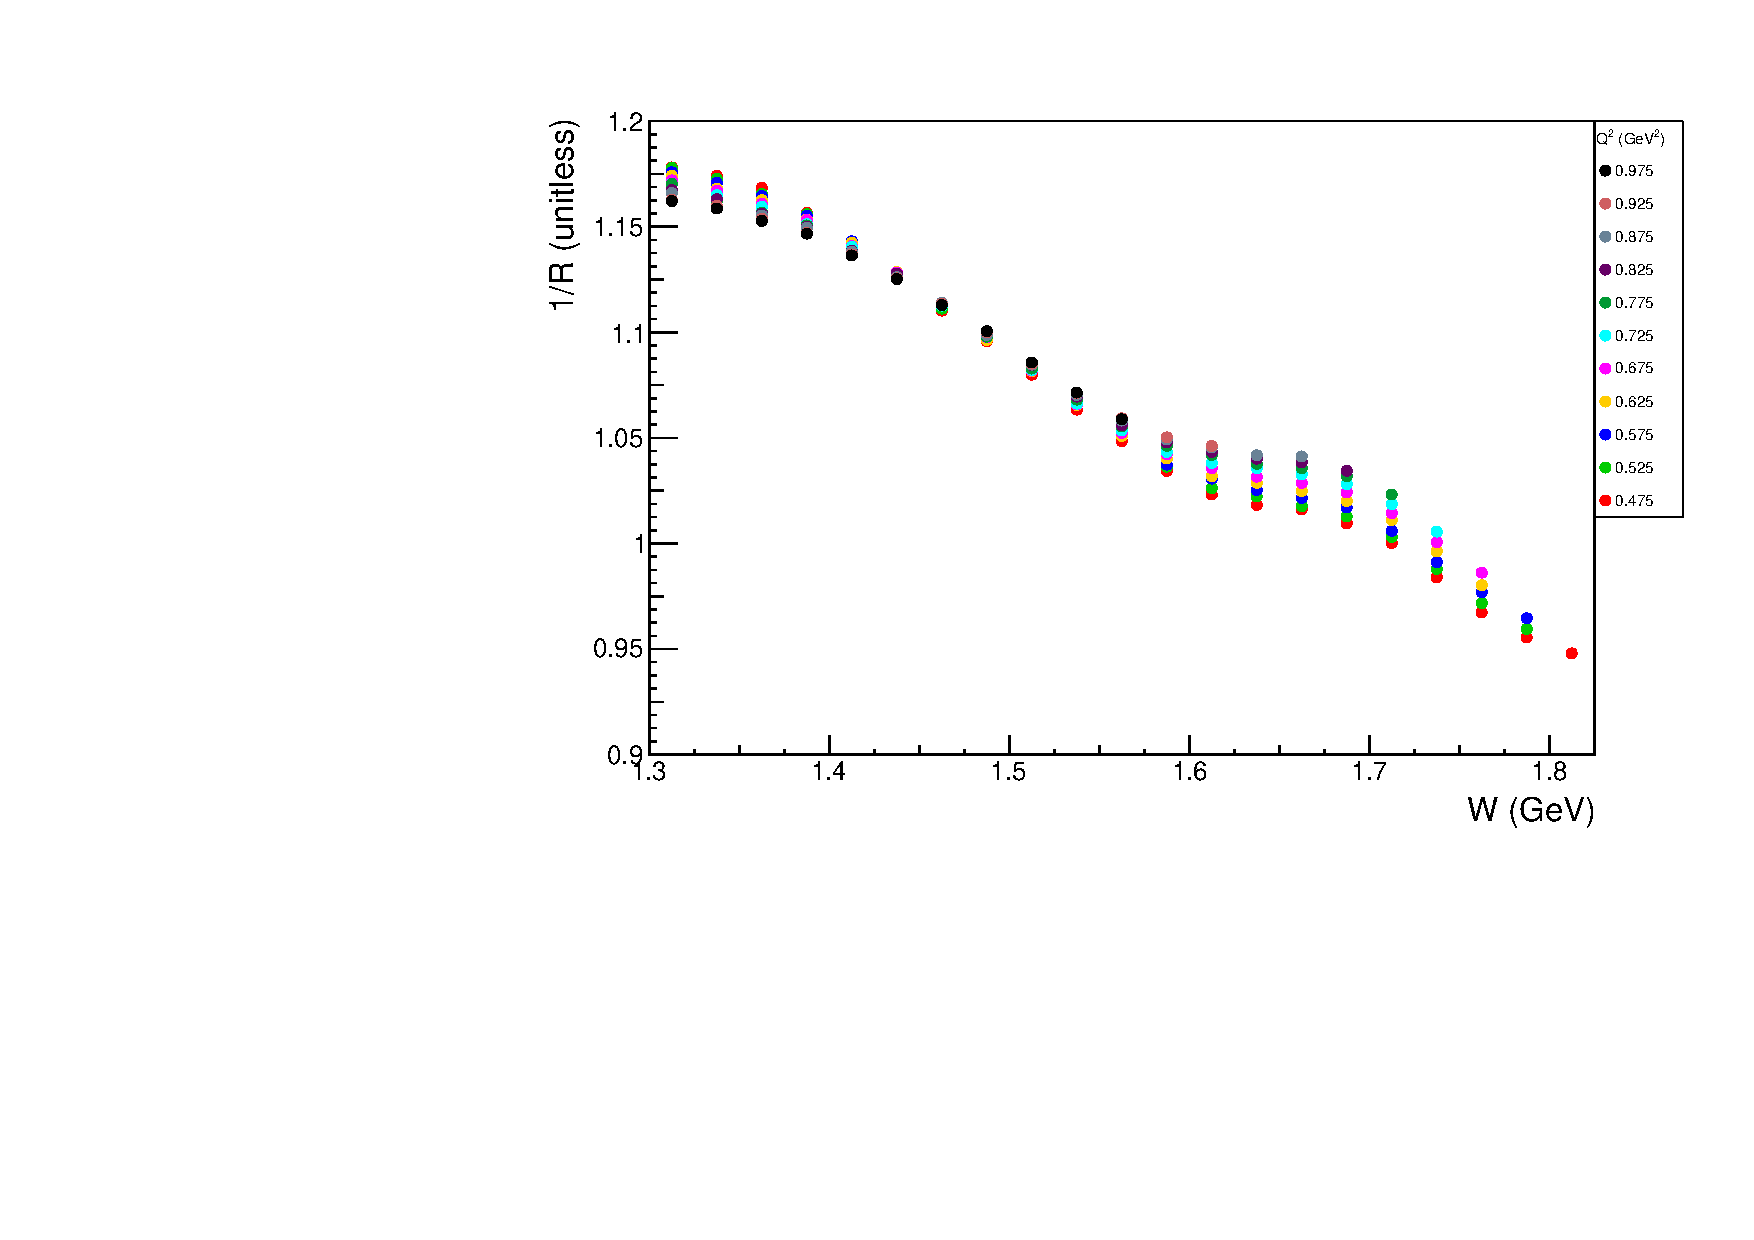
\includegraphics[width=13cm]{pictures/corrections/radcorr.pdf}
\caption{\small Reciprocal of the radiative correction factor ($1/R$) as a function of $W$ for different $Q^{2}$ bins (see Eq.~\eqref{eq:rad_corr}).} \label{fig:radcorr}
\end{center}
\end{figure}

This approach gives the correction factor $R$ only as a function of $W$ and $Q^{2}$, disregarding its dependence on the hadronic variables. However, the need to integrate the cross section at least over four hadronic variables (see Eq.~\eqref{inegr5diff}) considerably reduces the influence of the final state hadron kinematics on the radiative correction factor, thus justifying the applicability of the procedure~\cite{Mo:1968cg,twopeg,twopeg-d}.

The quantity $1/R$ is plotted in Fig.~\ref{fig:radcorr} as a function of $W$ for different $Q^{2}$ bins. The uncertainties associated with the statistics of generated events are very small and therefore not seen in the plot\footnote[3]{The total of about 2.5$\cdot 10^{9}$ either radiated or non-radiated events were generated in the investigated kinematic region for the calculation of the radiative correction factor.}. Note that the correction factor introduced in Fig.~\ref{fig:radcorr} is slightly different from that given in Ref.~\cite{Fed_an_note:2017} for the same beam energy of the free proton experiment ($E_{beam} = 2.039$~GeV). This difference comes from the fact that generated events in Eq.~\eqref{eq:rad_corr} are subjected to the smearing due to the Fermi motion of the target proton. 

Once this correction is applied, the extracted cross sections are treated as non-radiated, but Fermi-smeared.


\section{Unfolding the effects of the target motion}
\label{Sect:fermi_corr}


The motion of the target proton in a deuterium nucleus introduces into this analysis some specific issues that are not inherent for the previously conducted studies of the double-pion cross sections~\cite{Rip_an_note:2002,Ripani:2002ss,Fed_an_note:2007,Fedotov:2008aa,Isupov:2017lnd,Arjun,Fed_an_note:2017,Fed_paper_2018}. As was described in Sects.~\ref{Sect:excl_cut} and~\ref{Sect:smearing_blurring}, the intention to use in the analysis the $\pi^{-}$ missing topology (that serves the purpose of the cross section extraction best) leads inevitably to working under the target-at-rest-assumption. The latter, however, not only complicates the selection of exclusive events (see Sect.~\ref{Sect:excl_cut}), but also impacts the extracted cross sections due to the following reasons.

\begin{itemize}

\item  One has to use the smeared reaction invariant mass $W_{sm}$ for the cross section binning (see Sect.~\ref{Sect:smearing_blurring}). As a result, the extracted cross section is assigned to the $W$ value different from the actual one. This makes both integral and single-differential cross sections to be distorted. 

 
\item  One has to use an approximate Lab to CMS transformation that ignores the target motion (see Sect.~\ref{Sect:lab_cms}). This approximation introduces some inaccuracy to the measured angular ($\theta$, $\varphi$, and $\alpha$) distributions without having an impact on the invariant mass distributions and $W$ and $Q^{2}$ cross section dependencies due to their Lorentz invariance. 


\end{itemize}

The former effect is thought to have a much greater impact on the cross section than the latter. Thus, being folded with the aforementioned effects of the target motion, the extracted cross sections are seeking the corresponding unfolding correction. This correction is performed by means of two Monte Carlo event generators TWOPEG~\cite{twopeg} and TWOPEG-D~\cite{twopeg-d}. TWOPEG is the event generator for the double-pion electroproduction off the free proton that currently provides the best cross section estimation in the investigated kinematic region. TWOPEG-D is the event generator for the same exclusive reaction but off the proton that moves in the deuterium nucleus. This event generator was especially developed to be used in the studies, where the experimental information of the target proton momentum is inaccessible, and one is forced to work under the target-at-rest-assumption. TWOPEG-D convolutes the double-pion cross section with effects of the target motion and thus imitates the conditions of the experimental cross section extraction.

To calculate the correction factor, two samples of double-pion events produced either off the proton at rest and off the moving proton were generated (with TWOPEG and TWOPEG-D, respectively). Both event generators provide the particle's four-momenta written in the Lab system and distribute events according to the corresponding electron-scattering cross section. As the reaction invariant mass both samples use the value calculated from the initial particles (see Eq.~\eqref{W_fin_1}), which for the ``moving proton" events is calculated under the target-at-rest-assumption (as was done for the cross section calculation). The generated four-momenta are then subject to the transformation to the CMS. For both samples the transformation is performed according to the procedure given in App.~\ref{app_lab_cms_trans} for the case of the proton at rest. For the ``moving proton" sample, this approximation introduces in the event distributions the same inaccuracy as appears in the extracted cross sections. Then the kinematic variables are calculated and the generated events of both samples are binned in the same way as the extracted cross sections (see Sect.~\ref{Sect:binning}). 


\begin{figure}[htp]
\begin{center}
\framebox{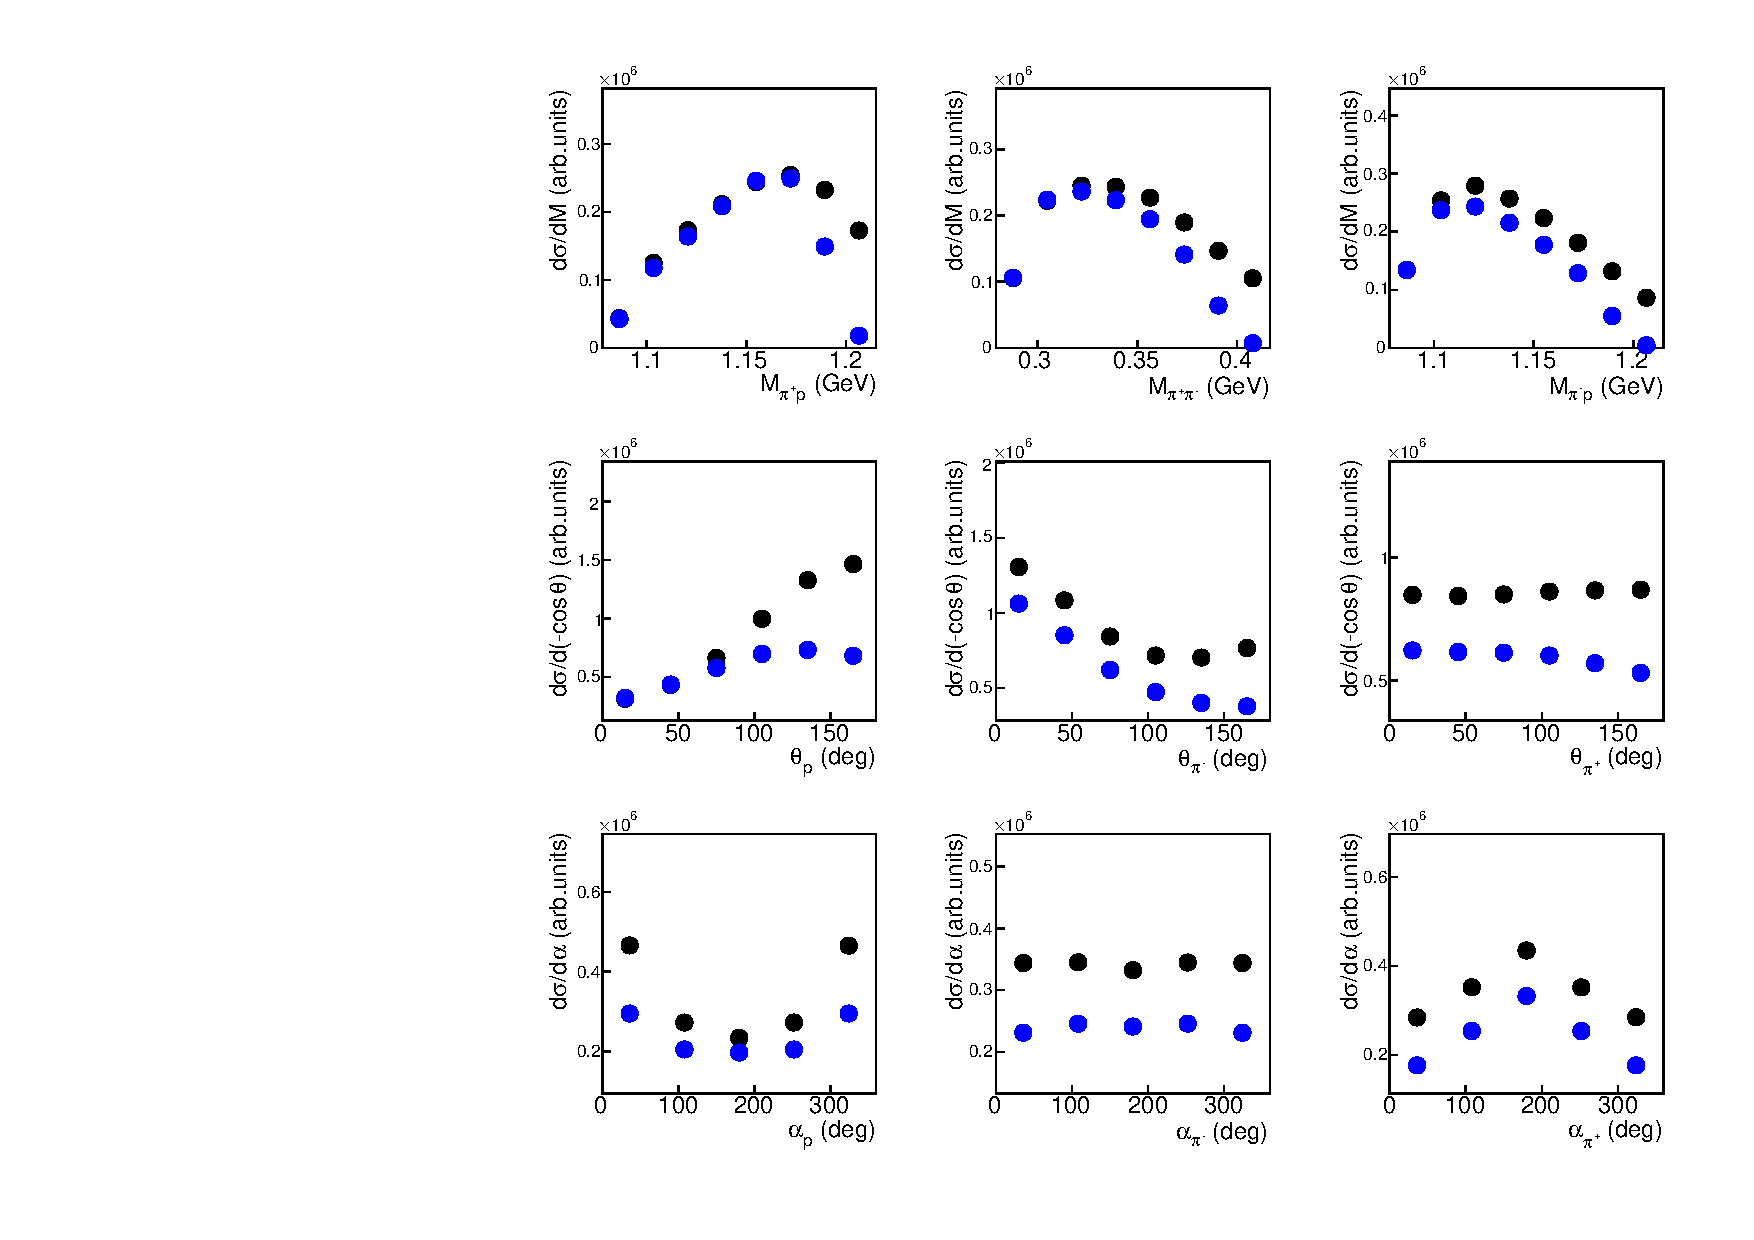
\includegraphics[width=12cm]{pictures/corrections/ferm_noferm_1diff_475_13375.pdf}}
\caption{\small Single-differential distributions of generated double-pion events produced off the proton at rest (blue symbols) and off the moving proton (black symbols). The former were generated with TWOPEG~\cite{twopeg} and the latter with TWOPEG-D~\cite{twopeg-d}. The example is given for the particular $\Delta W \Delta Q^{2}$ bin with the central point at $W=1.3375$~GeV and $Q^{2}=0.475$~GeV$^{2}$. As this bin is located near the threshold, the moving proton distributions (black symbols) have a high relative event excess comparing with the free proton distributions (blue symbols). See text for details. } \label{ferm_cor_1diff_1}
\end{center}
\end{figure}

Therefore, the distributions of events generated with TWOPEG-D acquire the same inaccuracies as the extracted cross sections, i.e. the value $W_{sm}$ is used for the binning and the approximate Lab to CMS transformations are applied. The manifestation of these inaccuracies differs depending on various final state variables and has a strong $W$-dependence as Figs.~\ref{ferm_cor_1diff_1} and~\ref{ferm_cor_1diff_2} demonstrate. These figures show the single-differential distributions of $\mathbb{N}_{nofermi}$ (blue symbols) and $\mathbb{N}_{fermi}$ (black symbols), which are the weighted numbers of events generated with TWOPEG and TWOPEG-D, respectively. In Fig.~\ref{ferm_cor_1diff_1} these distributions are shown for a low $W = 1.3375$~GeV, while in Fig.~\ref{ferm_cor_1diff_2} they are shown for a higher $W=1.5625$~GeV. The uncertainties associated with the statistics of generated events are very small and therefore not seen in the plots\footnote[4]{For each event sample the total of about 2.5$\cdot 10^{10}$ events were generated in the investigated kinematic region for the calculation of the correction factor.}.

\begin{figure}[htp]
\begin{center}
\framebox{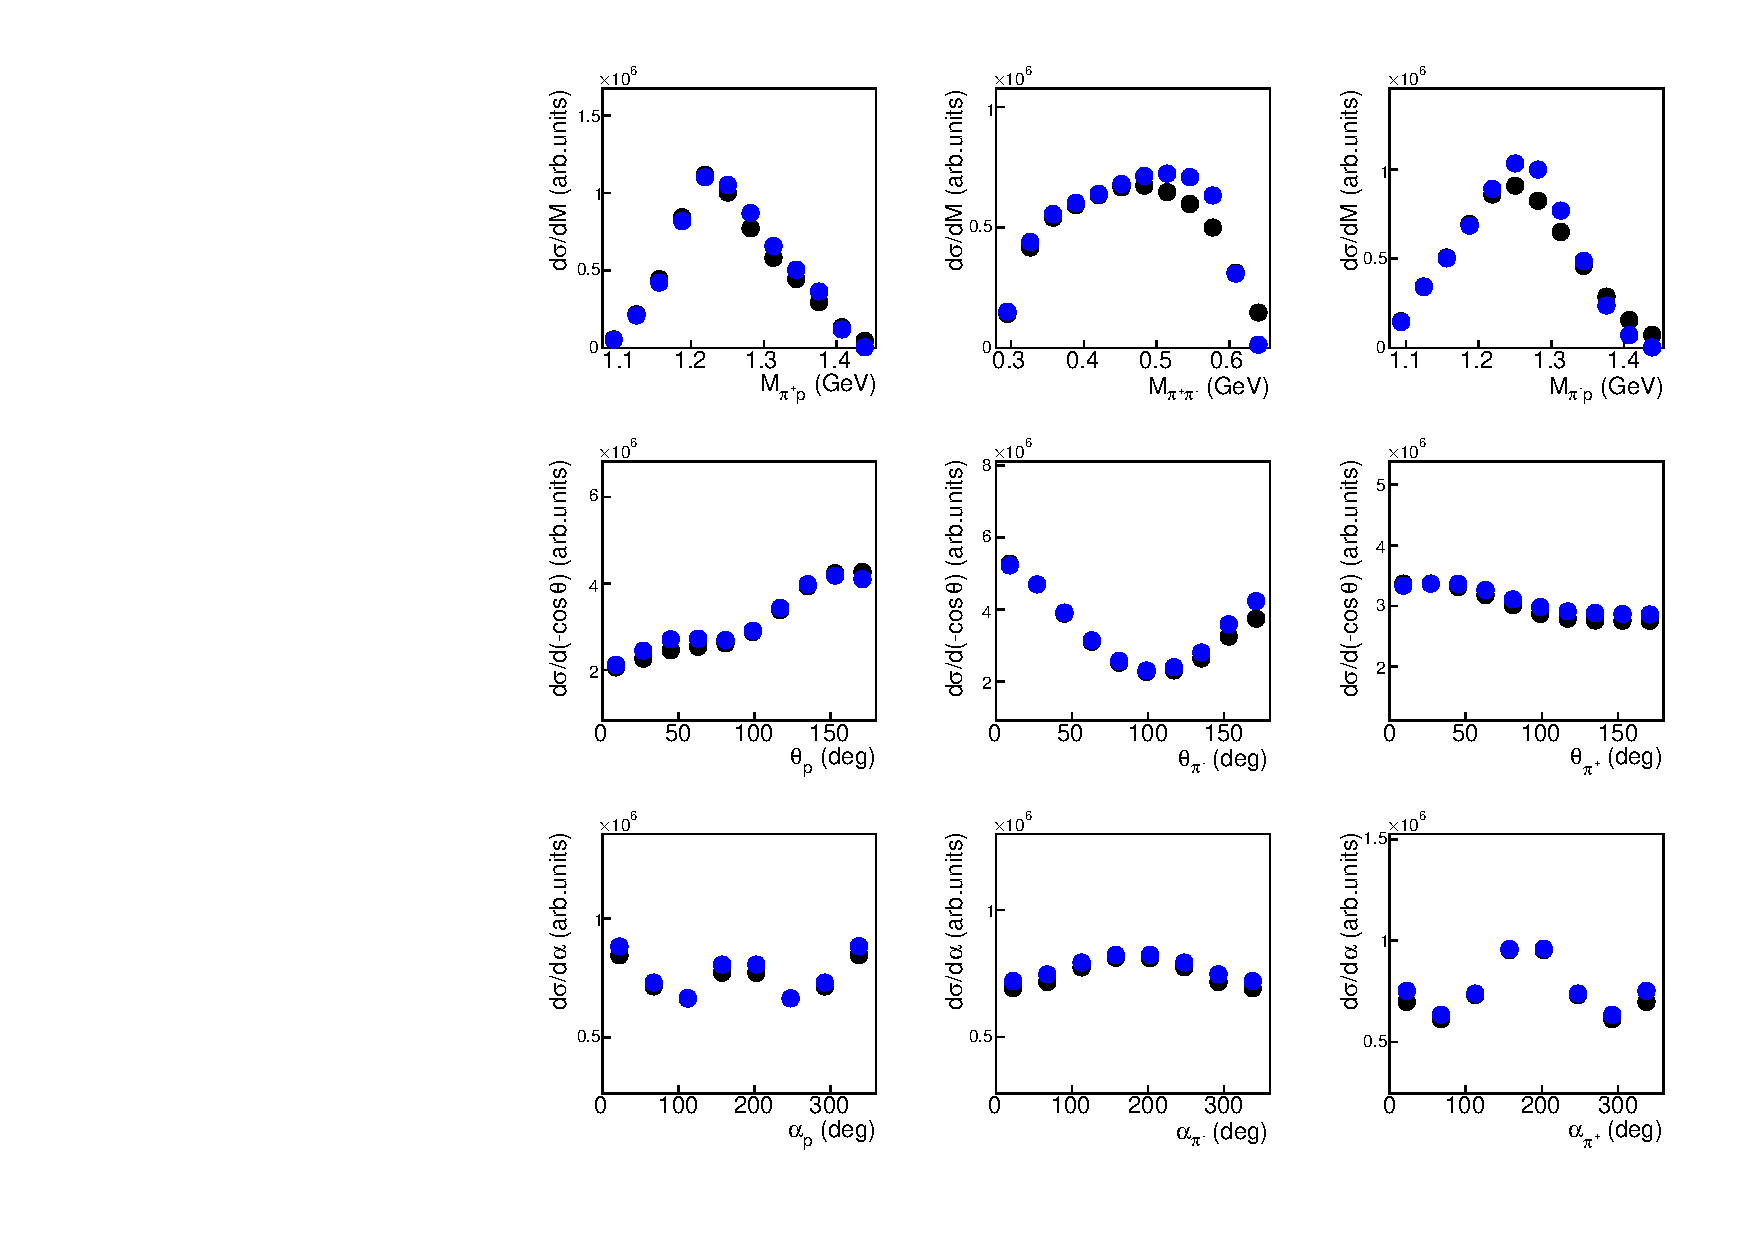
\includegraphics[width=12cm]{pictures/corrections/ferm_noferm_1diff_475_15625.pdf}}
\caption{\small Single-differential distributions of generated double-pion events produced off the proton at rest (blue symbols) and off the moving proton (black symbols). The former were generated with TWOPEG~\cite{twopeg} and the latter with TWOPEG-D~\cite{twopeg-d}. The example is given for the particular $\Delta W \Delta Q^{2}$ bin with the central point at $W=1.5625$~GeV and $Q^{2}=0.475$~GeV$^{2}$. As the bin is located in the peak region, the moving proton distributions (black symbols) have a small relative event deficit comparing with the free proton distributions (blue symbols). See text for details. } \label{ferm_cor_1diff_2}
\end{center}
\end{figure}

As seen from Figs.~\ref{ferm_cor_1diff_1} and~\ref{ferm_cor_1diff_2}, the target motion considered under the itemized conditions listed above affects mostly the cross section near the threshold, while for higher $W$ their impact is significantly less pronounced. This happens due to the following. Let's consider a particular $W_{true}$ bin. As shown in Ref.~\cite{twopeg-d}, each value of $W_{true}$ corresponds to a sequence of $W_{sm}$ values, which are symmetrically scattered in the vicinity of $W_{true}$ with a spread of 50-100 MeV. This leads to the fact that the same bin in $W_{sm}$ has a different number of events compared to the $W_{true}$ bin. This difference depends on the cross section behavior in the vicinity of 50-100 MeV of this bin. The cross section abruptly rises from the threshold with a strong convex nonlinearity, which smooths as $W$ grows up to 1.4~GeV, and then turns to a concave nonlinearity forming the left slope of the resonance peak at 1.5~GeV. Then the cross section modestly increases and decreases several times changing its nonlinearity type. In any $W_{true}$ subrange the cross section can be written as $a + f(W)$, where $a=const$, while $f(W)$ evolves from zero and determines the cross section nonlinearity within the subrange.  Then the absolute variation in the event number in $W_{sm}$ bin is determined solely by the nonlinearity of the function $f(W)$, i.e. convex nonlinearity leads to an event excess in the bin, while concave nonlinearity -- to an event deficit. Hence, in the resonance peaks an event deficit is observed, while the region close to the threshold and the dip between the peaks have an event excess. However, the relative event variation depends on $a$ and is higher for smaller $a$. The smallest value of $a$ is reached at the threshold ($a = 0$), therefore the near-to-threshold subrange has the greatest relative variation of event number.



Indeed, in Fig.~\ref{ferm_cor_1diff_1}, which is plotted for the $W$ bin located close to the threshold, the moving proton distributions (black symbols) have a high relative event excess compared to the free proton distributions (blue symbols). Meanwhile, in Fig.~\ref{ferm_cor_1diff_2}, which is plotted for the $W$ bin located at the peak region, the moving proton distributions (black symbols) have small relative event deficit comparing with the free proton distributions (blue symbols). 

For the low $W$ region (as in Fig.~\ref{ferm_cor_1diff_1}) it is noteworthy that a very large relative difference between the free proton and the moving proton cross sections is observed for the right part of the invariant mass distributions. This happens due to the phase space broadening with $W$ that takes place for invariant masses (see App.~\ref{app_ph_space}). The invariant mass distribution typically has a maximum in the middle and gradually goes to zero on both edges. The lower the $W$ value is, the narrower is the distribution width. As $W$ grows, the distribution widens to the right and goes to zero farther away. Meanwhile, each bin in $W_{sm}$ contains a mixture of events with the values of $W_{true}$ spread within 50-100~MeV near this bin. For low $W$ this spread is comparable with the total  width of the invariant mass distribution. Therefore, the right distribution side acquired the event excess that comes from the same bins in invariant mass but located at higher $W_{true}$ and hence having high cross sections.


The unfolding correction is performed in each multi-dimensional bin of the double-pion production phase-space (see Sect.~\ref{Sect:kin_var} as well as App.~\ref{app_ph_space}), i.e. in each $\Delta W \Delta Q^{2}\Delta^{5}\tau$ bin the cross section is divided by the correction factor $\mathcal{F}$ (see  Eq.~\eqref{expcrossect}) that is calculated as
\begin{equation}
\mathcal{F}(\Delta W, \Delta Q^{2},\Delta^{5}\tau) = \frac{\mathbb{N}_{fermi}}{\mathbb{N}_{nofermi}},
\label{eq:ferm_corr}
\end{equation}
where $\mathbb{N}_{nofermi}$ and $\mathbb{N}_{fermi}$ are the weighted numbers of generated double-pion events in the $\Delta W \Delta Q^{2}\Delta^{5}\tau$ bin produced off the proton at rest and off the moving proton, respectively. Both event samples were generated without radiative effects, since the correction factor $\mathcal{F}$ is applied to the cross sections that are already corrected for the radiative effects (see Sect.~\ref{Sect:rad_corr}).


The impact of the unfolding correction on the extracted integral cross sections is illustrated in Fig.~\ref{ferm_cor_nocor_int}, where the distributions before the correction are plotted in orange, while the distributions after the correction are plotted in dark blue. The comparison is given for two $Q^{2}$ bins. As was expected, the correction causes a slight cross section increase in the resonance peaks and a decrease near the threshold and in the dip between the peaks. 

\begin{figure}[htp]
\begin{center}
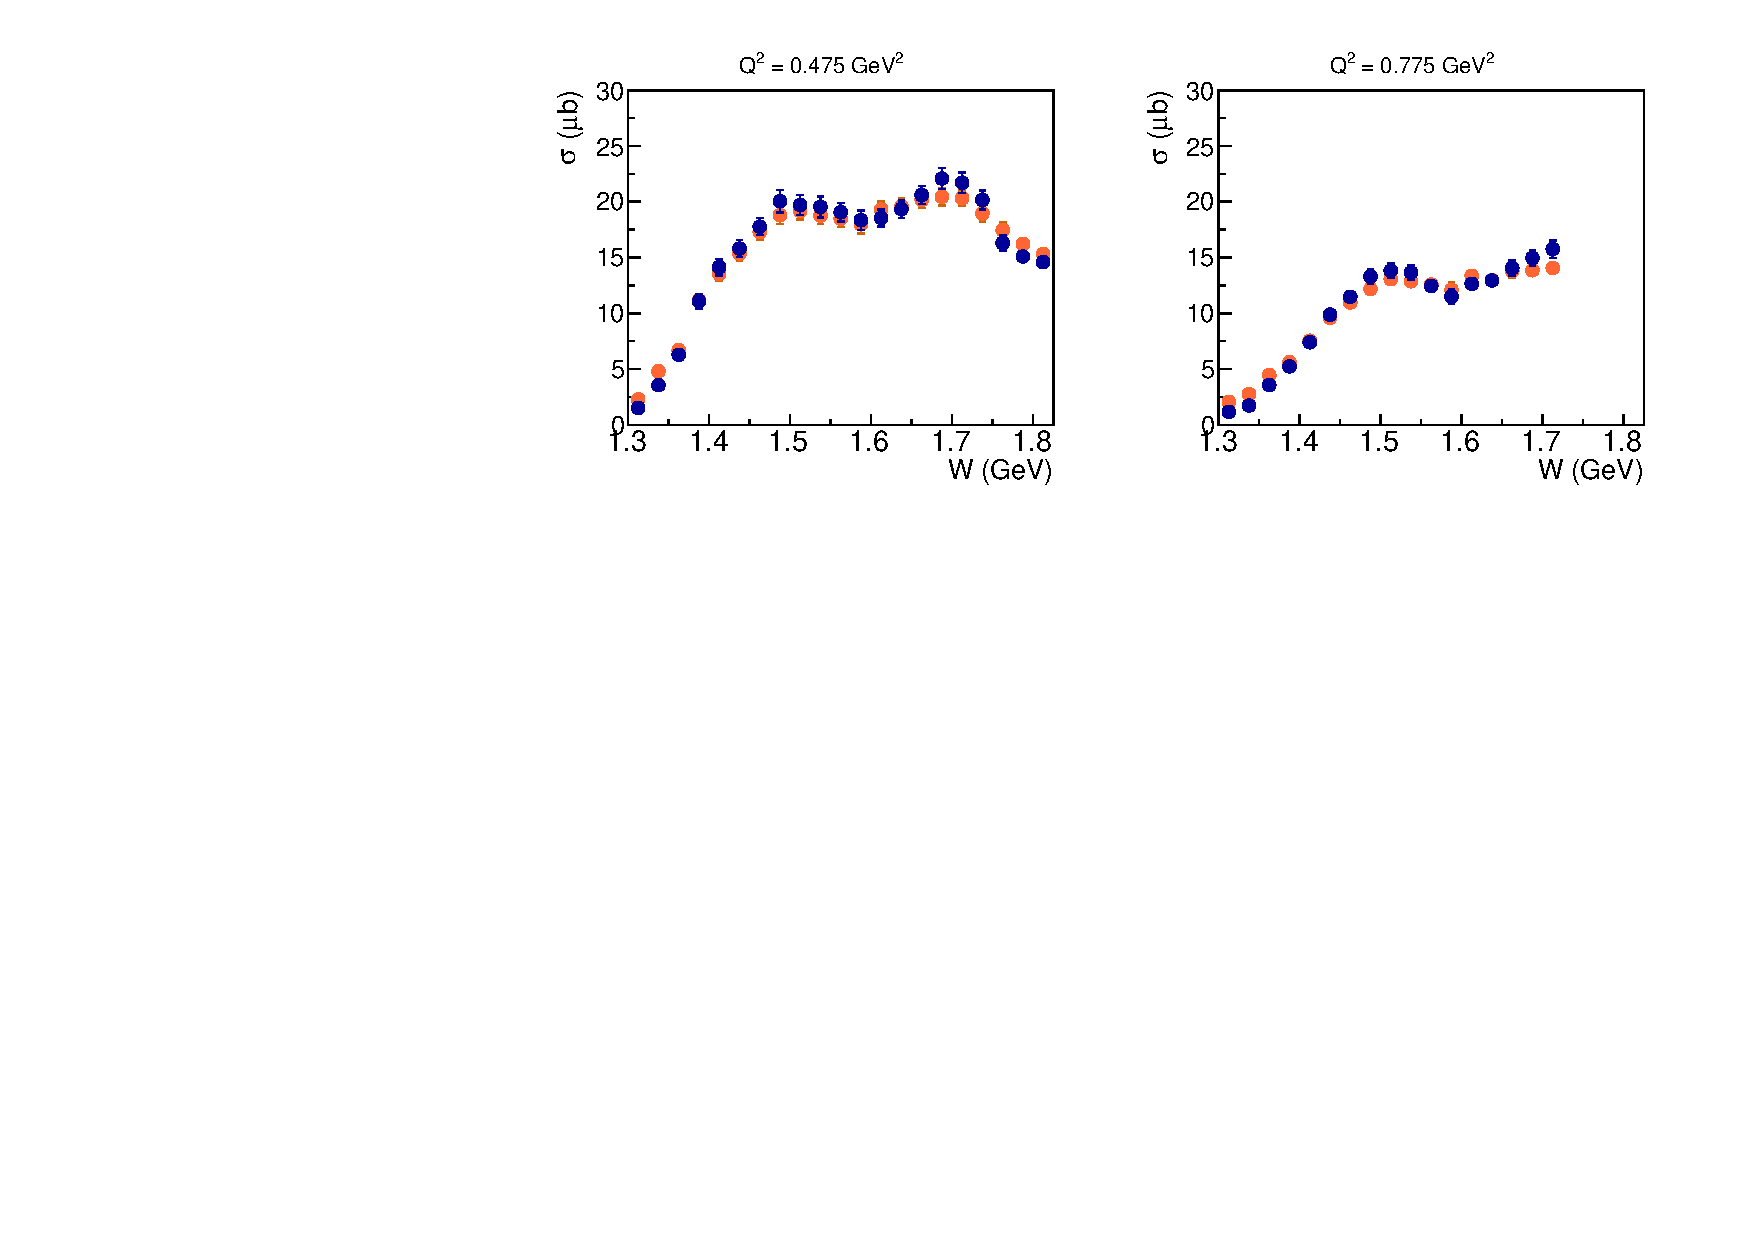
\includegraphics[width=14cm]{pictures/corrections/fermi_cor_nocor_int.pdf}
\caption{\small Impact of the unfolding correction on the extracted integral cross sections. The cross section before the correction is plotted in orange, while the cross section after the correction is plotted in dark blue (both are divided by the virtual photon flux). The comparison is given for two $Q^{2}$ bins as specified above the plots. } \label{ferm_cor_nocor_int}
\end{center}
\end{figure}

The value of the correction factor in Eq.~\eqref{eq:ferm_corr} depends on both the free proton cross sections and the model of the deuteron wave function that were employed in the event generators. The former relies strongly on the JM model fit of the available data on double-pion cross sections, while for the latter the Bonn model was used (see Refs.~\cite{twopeg,twopeg-d} for more detail). Therefore, the uncertainty of the extracted cross sections that comes from this unfolding correction is attributed to the model dependence uncertainty and is discussed in Sect.~\ref{Sect:mod_dep}. 

Once corrected for the effects of the target motion and then divided by the virtual photon flux, the cross section is treated as the true virtual photoproduction cross section and is attributed to the central point of the corresponding $\Delta W \Delta Q^{2}\Delta^{5}\tau$ bin.


\section{Correction for binning effects}
\label{Sect:bin_cor}

The cross section, extracted in bins of a finite size, is assigned to the central point of a bin. On this way the cross sections acquire binning caused distortions and, therefore, are seeking the corresponding corrections. In this section, which is devoted to the binning effects, two separate binning issues are distinguished, i.e. (i) the specific issue of affecting the cross section value in the next to last point of the invariant mass distributions and (ii) the common binning issue that impacts the cross section value in any bin of finite size. 

Let's address the specific binning issue in the invariant mass distributions first. As shown in Sect.~\ref{Sect:binning}, the binning in invariant mass requires special attention due to the broadening of the reaction phase-space with $W$ (see App.~\ref{app_ph_space}) and the corresponding $W$ dependence of the upper boundary of the invariant mass distributions (see Eq.~\eqref{eq:inv_mass_boundary}). This effect makes the upper boundary $M_{upper}$ to be indistinct, since the cross section is calculated in a bin $W_{left} < W < W_{right}$. To deal with this difficulty, the value of $M_{upper}$ is calculated using $W_{center}$, the center of the $W$ bin. Then a specific arrangement of mass bins is used, which forces the last bin to be situated completely out of the boundaries given by Eq.~\eqref{eq:inv_mass_boundary} using $W_{center}$. When integrating the cross section over the mass distribution, the events in the extra bin are included, but a cross section for this bin is not reported.


Meanwhile, the cross section in the next to last bin (labeled as bin number $N_{bins}-1$) should be treated carefully. This is best illustrated in Fig.~\ref{fig:mass_corr}, which shows schematically the event distribution in mass, ending in $M_{upper}$ for three choices of $W$ at $W_{left}$ (dot-dashed), $W_{center}$ (solid) and $W_{right}$ (dashed). The black points at $M^{N_{bins}-1}_{left}$ and $M^{N_{bins}-1}_{right}$ show the left and right boundaries of the next to last bin, respectively. In the next to last bin events with $W < W_{center}$ are distributed over a range, which is less than $\Delta M$ defined by Eq.~\eqref{eq:bin_width}. However, when extracting the cross sections, the event yield was divided by the full bin width $\Delta M$, thus leading to an underestimation of the cross section.



\begin{figure}[htp]
\begin{center}
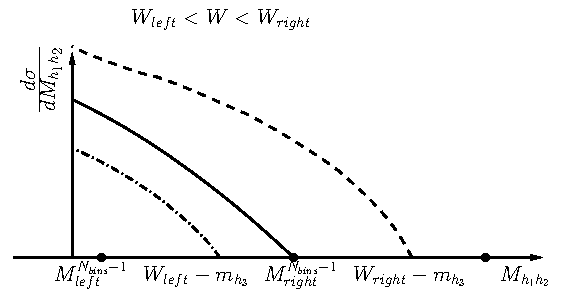
\includegraphics[width=12cm]{pictures/corrections/mass_tex.pdf}
\caption{\small  Schematic representation of the invariant mass distributions ending in $M_{upper}$ calculated according to Eq.~\eqref{eq:inv_mass_boundary} for three choices of $W$ at $W_{left}$ (dot-dashed), $W_{center}$ (solid) and $W_{right}$ (dashed). The black points at $M^{N_{bins}-1}_{left}$ and $M^{N_{bins}-1}_{right}$ show the left and right boundaries of the next to last bin, respectively, while the remaining point marks the right boundary of the last mass bin.} \label{fig:mass_corr}
\end{center}
\end{figure}


The correction for this effect was taken from Ref.~\cite{Fed_an_note:2017,Fed_paper_2018}. It was made using the TWOPEG double-pion event generator~\cite{twopeg}. The correction factor to the cross section in the next to last bin is the ratio of the simulated cross sections calculated with fixed $\Delta M$ defined by Eq.~\eqref{eq:bin_width} and with $\widetilde{\Delta M} = W-m_{h_{3}} - M^{N_{bins}-1}_{left}$, which was different for each generated event. This factor provides the correction to the cross section in the next to last bin that varied from $\sim$5\% to $\sim$10\%.


Let's now address the common binning issue that impacts the cross section value in any bin of a finite size. Extracted in a finite bin, the cross section is subject to averaging within this bin. For instance, if there is a sharp peak in the middle of a bin, then the average value of the cross section in that bin will always be smaller than the peak value. Any non-linear behavior of the cross section will likely result in an offset of the obtained value. There are two methods of correcting this offset, i.e. (i) to correct the kinematic quantities associated with the bin and use the corrected values instead of the central values or (ii) to correct the cross section value in the center of the bin. Both these methods are widely used for the binning corrections. In the studies of double-pion cross sections, however, the second method has become conventional~\cite{Fed_an_note:2007,Fedotov:2008aa,Fed_an_note:2017,Fed_paper_2018}. Therefore, in this study the second method is chosen, in order to keep the initial binning over the kinematic variables and to facilitate the cross section comparison with the results obtained off the proton at rest~\cite{Fed_an_note:2017,Fed_paper_2018}.

In this study one-dimensional binning corrections are performed, i.e., the cross section dependence on each kinematic variable $x$ is corrected individually (where $x$ corresponds to $W$, $Q^{2}$, and hadron variables). In any one-dimensional bin $[x_{min},x_{max}]$ the cross section value is multiplied by the correction factor $C_{bin}$. To estimate this factor some assumptions about the cross section behavior within the bin are needed, and hence, the cross section shape should be described by a continuous function $f(x)$. The multiplicative correction factor $C_{bin}$ is then calculated in each bin $[x_{min},x_{max}]$ as
\begin{equation}
\begin{aligned}
%\sigma_{corr} & = &\sigma_{uncorr} \times
%C_{bin} & \text{ \,\,with}\\
\label{eq:bincor}
C_{bin} & = &\frac{f(x_{center})}{\int\limits_{x_{min}}^{x_{max}} f(x)dx} \textrm{ ,}
\end{aligned}  
\end{equation}
where $x_{center}$ is the central point of the $[x_{min},x_{max}]$ bin.






For the single-differential distributions a cubic spline approximation is chosen to continuously describe the cross section shape, as shown in Fig.~\ref{fig:bin_cor_1d}. The black and red points in this figure are the cross sections before and after binning corrections, respectively, and the curves correspond to the spline approximation. For the invariant mass and $\theta$ angular distributions the splines are forced to pass through the intermediate points that are obtained by averaging over two neighboring cross section points. This method reduces the splines sensitivity to accidental cross section fluctuations. Beside this, for the invariant mass distributions the splines are required to give zero at the distribution edges. For the $\alpha$ angular distributions the splines are forced to pass through the points that are obtained by averaging over two cross section points symmetrical with respect to $\alpha = 180^{\rm o}$. This approach reflects the fact that after the integration over $\varphi$, the cross section must be symmetrical in the $\alpha$ angle (meanwhile, the extracted experimental distributions are slightly asymmetrical)\footnote[5]{Although the $\varphi$ distributions are not reported here, they were nevertheless extracted and added to the CLAS physics database~\cite{CLAS_DB}. The $\varphi$ distributions were thus subjected to the binning correction with the same approach used for the $\theta$ distributions.}.

\begin{figure}[htp]
\begin{center}
\framebox{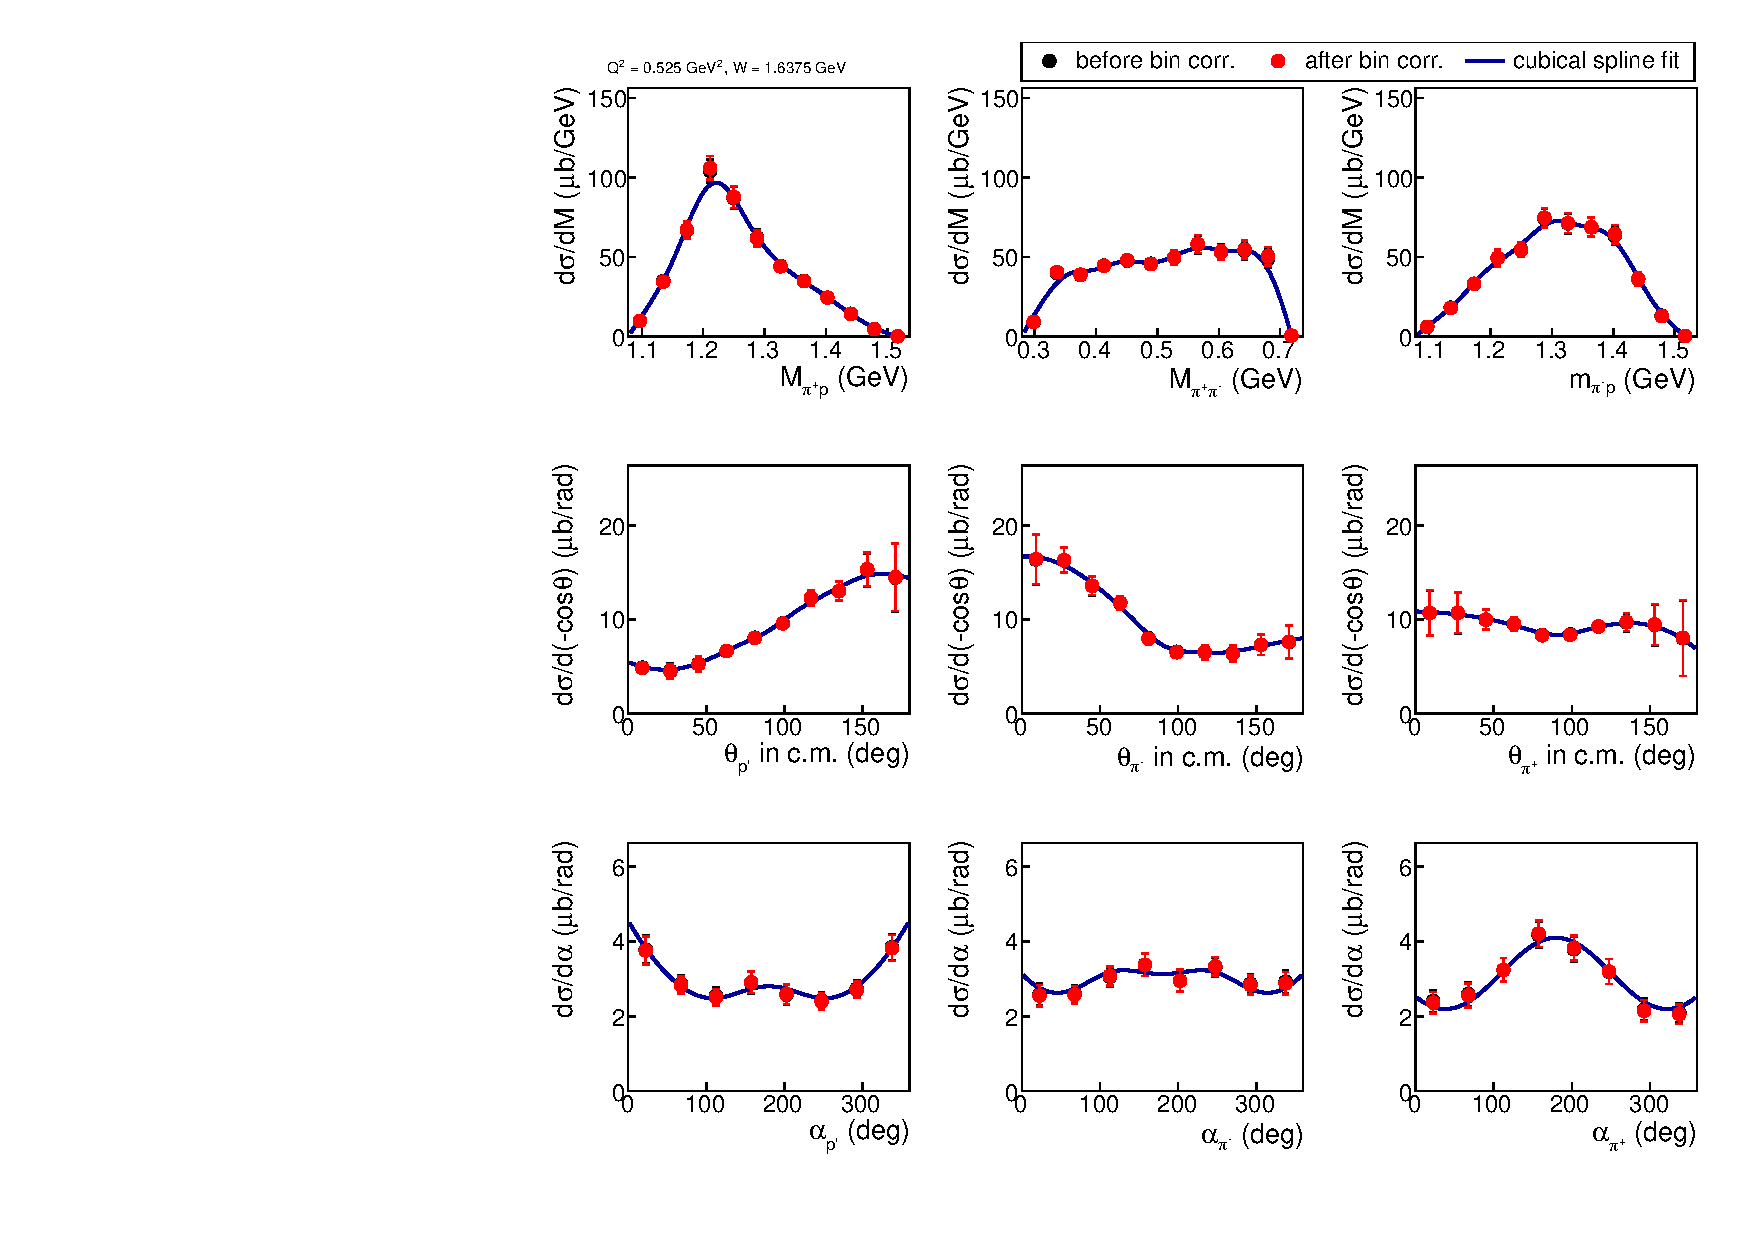
\includegraphics[width=13.5cm]{pictures/corrections/bin_cor_1d.pdf}}
\caption{\small Single-differential cross sections as functions of the final hadron variables before (black points) and after (red points) the binning corrections. Curves represent a cubic spline approximation. The example is given for a particular $\Delta W \Delta Q^{2}$ bin with the central point $W=1.6375$~GeV and $Q^{2}=0.525$~GeV$^{2}$.  } \label{fig:bin_cor_1d}
\end{center}
\end{figure}



The integral cross sections are subjected to individual corrections of the $Q^{2}$ dependence inside the $W$ bins and the $W$ dependence inside the $Q^{2}$ bins, as shown on the left and right plots of Fig.~\ref{fig:bincor_w_q2}, respectively. In this figure black and red points represent the cross section values before and after binning corrections, respectively, while the curves correspond to the continuous cross section approximation. The latter are based on a second order polynomial fit of the $Q^{2}$ distributions (left plot) and on a cubic spline approximation for the $W$ distributions (right plot). The splines are forced to pass through the intermediate points that are obtained by averaging over two neighboring cross section points. In this way, the integral cross section value in each $\Delta W\Delta Q^{2}$ bin acquires two multiplicative correction factors. The corrections obtained for the integral distributions are then propagated to the single-differential cross sections.

\begin{figure}[htp]
\begin{center}
\includegraphics[width=8cm]{pictures/corrections/bin_cor_q2.pdf}
\includegraphics[width=8cm]{pictures/corrections/bin_cor_w.pdf}
\caption{\small $Q^{2}$ dependence (left plot) and the $W$ dependence (right plot) of the integral cross sections before (black points) and after (red points) the binning corrections. The curves correspond to a second order polynomial fit for the left plot and a cubic spline approximation for the right one. Each distribution is plotted for one particular bin as specified above the plots.} \label{fig:bincor_w_q2}
\end{center}
\end{figure}
 
Since in this analysis a relatively fine binning in all kinematic variables is chosen (see Sect.~\ref{Sect:binning}), the effect of the binning corrections is almost insignificant. 
This is why in Figs.~\ref{fig:bin_cor_1d} and~\ref{fig:bincor_w_q2} the black points (before the correction) are almost completely covered by the red ones (after the correction). For the $Q^{2}$ dependences the correction factors are less than 1\% in all bins, and for the $W$ dependences they are $\sim$2\%-3\% for the first two low $W$ bins and less than 1\% in all other bins. For the single-differential distributions, the corrections are on the level of 1\%-2\% for the majority of bins, but rise for some points (mostly at low $W$) up to 5\%-6\%.


\chapter{Other issues}
\label{Sect:issues}


\section{The cross section dependence on the beam energy}


The phi-integrated virtual photoproduction cross section $\sigma_{v}$ can be decomposed into the combination of the structure functions\footnote[1]{The full decomposition (for the case of the unpolarized electron beam) can be found e.g. in Refs.~\cite{twopeg,Skorodumina:2016pnb}.},
\begin{equation}
\sigma_{v} = \sigma_{T} + \varepsilon_{L}\sigma_{L}\text{~~~with~~~}\varepsilon_{L}=\frac{Q^{2}}{\nu^{2}}\varepsilon_{T},\label{eq:beam_en_dep}
\end{equation}
where $\sigma_{T}$ and $\sigma_{L}$ are the transverse and longitudinal structure functions, respectively, while $\varepsilon_{L}$ is the longitudinal polarization of the virtual photon with $\varepsilon_{T}$ given by Eq.~\eqref{polarization}.

Being decomposed in this way, the cross section $\sigma_{v}$ has a specific beam energy dependence, which is incorporated into the coefficient $\varepsilon_{L}$. The structure functions themselves, meanwhile, do not depend on the beam energy. A single experiment conducted with a certain beam energy allows for the extraction of $\sigma_{v}$ as a whole without accessing the separate structure functions. Thus, the beam energy dependence turns out to be implicitly incorporated into the extracted cross sections.

Although the experiment is conducted with a fixed value of the laboratory beam energy, the actual energy of the incoming electron involved in the reaction turns out to alter and differ from the fixed laboratory value due to  (i) the radiative effects that electrons undergo and (ii) the Fermi motion of the target proton. As a consequence, the extracted cross section cannot be associated with a distinct value of the electron beam energy, and this may complicate the interpretation of the results. Let's address these issues in more detail. 

\begin{itemize}


\item [(i)] The incoming and scattered electrons can emit photons thus reducing their energy. Due to the change of the incoming electron energy, the extracted cross sections correspond to the superposition of various beam energies. The correction due to this effect is included into the procedure of radiative corrections (see Sect.~\ref{Sect:rad_corr}).


\item [(ii)] The experiment off the moving proton with fixed laboratory beam energy corresponds to that off the proton at rest performed with varying effective beam energies~\cite{twopeg-d}. As a result, the extracted cross sections off moving protons are convoluted with the dependence of the quantity  $\varepsilon_{L}$ on the beam energy (see Eq.~\eqref{eq:beam_en_dep}). A study in Ref.~\cite{twopeg-d}, however, proves that this effect has an insignificant influence on the cross section. The correction due to this effect (which is negligible anyway) is automatically included into the procedure of unfolding the effects of the target motion (see Sect.~\ref{Sect:fermi_corr})\footnote[2]{Note that the radiative effects decrease the beam energy, while the Fermi motion leads to a symmetrical spread of the effective beam energy around the laboratory value.}. 


\end{itemize}



Being corrected, the cross sections extracted in this analysis may be assigned to the distinct value of the laboratory beam energy of $E_{beam} = 2.039$~GeV.
%However, in the experiment the information on these emissions is lost, and one has to assume the electron energy to be unchanged, thus introducing a systematic distortion to the extracted cross sections.

%Electron scattering off the moving proton performed with the beam energy $E_{beam}$ corresponds to that off the proton at rest conducted with the effective beam energy $\widetilde{E}_{beam}$, which is determined by the boost from the Lab frame to the quasi-Lab system, where the proton is at rest, while the incoming electron moves along the $z$-axis~\cite{twopeg-d}. This effective beam energy thus depends on the Fermi momentum of the target proton and differs event by event. Therefore, the experiment off the moving proton with the fixed electron beam energy corresponds to that off the proton at rest performed with the altered beam energy.


%The virtual photoproduction cross sections $\sigma_{v}$ has a specific beam energy dependence, which originates from two sources. The first source is the explicit beam energy dependence of the quantities $\Gamma_{v}$ and $\varepsilon_{T}$, which are given by Eq.~\eqref{flux} and Eq.~\eqref{polarization}, respectively. In the proton at rest experiments the conventional practice is to determine these two quantities in the Lab frame, where the electron beam has the fixed energy. Generally speaking, in the experiments off moving protons these quantities should be determined in the quasi-Lab system, and altered event by event value of the effective beam energy should be used in the calculations. Beside that, the $\sigma_{v}$ has also an implicit dependence on the beam energy that is incorporated into the coefficient $\varepsilon_{L}$ of the cross section decomposition into the transverse and longitudinal parts ($\sigma = \sigma_{T}+\varepsilon_{L}\sigma_{L}$). Therefore, in the moving proton experiments the $\sigma_{v}$ turns out to be convoluted with the dependencies of the quantities $\varepsilon_{T}$, $\varepsilon_{L}$, and $\Gamma_{v}$ on the beam energy. As a consequence, the extracted cross section cannot be associated with the distinct value of the electron beam energy that may complicate the interpretation of the result and its comparison with the cross sections of the proton at rest experiment.

%This question is addressed in detail in Ref.~\cite{twopeg-d}. This study proves that the convolution of the cross section with the dependencies of the quantities $\varepsilon_{T}$, $\varepsilon_{L}$, and $\Gamma_{v}$ on the beam energy has an insignificant influence on it.


%In this analysis the cross section is calculated ignoring its beam-energy dependence, i.e. the quantities $\varepsilon_{T}$ and $\Gamma_{v}$ were calculated in the Lab frame using the fixed laboratory value of the beam energy $E_{beam}$ = 2.039 GeV. The correction due to this approximation (which is negligible anyway) is automatically included into the procedure of unfolding the effects of the target motion (see Sect.~\ref{Sect:fermi_corr}). Being corrected, the extracted cross sections may be assigned to a distinct value of the laboratory beam energy.



\section{Off-shell effects}

The target proton is bound in the deuterium nucleus and thus undergoes nucleon-nucleon interactions. The nucleon mass, however, is thought to be an interaction-dependent quantity, i.e. the nucleon's physical mass in a nucleus is smaller than that of a free nucleon~\cite{Noble:1980my}. In other words, the target proton bound in the deuteron is off-shell, which means that its four-momentum squared is not equal to its mass squared.

In the study~\cite{Ye_Tian:2017}, which aimed at $\pi^{-}$ electroproduction off the neutron in deuterium, the impact of the off-shell effects on the measured cross sections was shown to be marginal. In this study the off-shell effects are ignored.




%\setcounter{chapter}{5}
\chapter{Normalization verification}
\label{Sect:norm}
\counterwithin{equation}{chapter}

To prove the credibility of an extracted observable, some well-established quantity is commonly used as a reference point. For this purpose one can use already published measurements of this observable, if they exist in the desired kinematic region, but this usually is not the case. Alternatively, one can focus on some quantity, which can be reliably approximated in this kinematic region by a theoretical model or parameterization. 
This auxiliary quantity is then extracted from the analyzed dataset, and the comparison of the measured value with the approximated one allows the reliability of the main result to be judged.

For experiments off a free proton, the elastic cross section usually serves as such a reference quantity as it can be approximated in a wide kinematic region by Peter Bosted parameterization with an excellent accuracy of a few percent, as Ref.~\cite{note_QE_peak}  demonstrates (see App. B there). Therefore an agreement between the auxiliary measured elastic cross section with the parameterized one, if achieved indicates both the correct normalization of the main result and the trustworthy quality of the electron selection.


Meanwhile, for experiments off a deuterium target, the quasi-elastic cross section off nucleons can serve as the corresponding reference quantity. 
However, this observable, if compared with the elastic free proton cross section, is less understood and lacking the same quality of theoretical description~\cite{note_QE_peak}. Nonetheless, several techniques have been developed in this matter with the Bosted parameterization of the deuteron quasi-elastic peak being the most commonly used tool.


%To prove the correct normalization of the obtained results, one is used to carry out a comparison with previously existing data (if they exist in the desired kinematic region) or some theoretical calculations/parameterizations. In the latter case, one usually concentrates on some well-understood and easily-measurable quantities such as the elastic cross section off free proton or quasi-elastic cross section off nucleons in nuclei.

%Nowadays, the elastic cross section off a free proton is well-known over a wide kinematic range, since it has been intensively studied experimentally for decades and eventually almost perfectly described by parameterizations. Meanwhile, the quasi-elastic cross section off nucleons is less understood and lacking the same quality of theoretical description. However, several techniques have been developed on this matter, which includes the Bosted parameterization of the deuteron quasi-elastic peak~\cite{Bosted_fit,Bosted:2007xd}.


Ref.~\cite{note_QE_peak} gives some details on the performance of the Bosted parameterization of the deuteron quasi-elastic peak~\cite{Bosted_fit,Bosted:2007xd} and tests its ability to describe experimental data by comparing the parameterized cross sections with published measurements~\cite{Hanson:1973vf,Rock:1991jy,Rock_SLAC}. This testing, being performed in the $Q^{2}$ range from $\sim$0.3~GeV$^2$ to $\sim$4~GeV$^2$, is of great importance for the current analysis as its $Q^{2}$ coverage falls within this range.


As follows from Ref.~\cite{note_QE_peak}, the Bosted parameterization in its default implementation systematically overestimates the measured integrals under the quasi-elastic peak and the overall description quality gradually decreases from several percent to almost 20\% as $Q^2$ grows from 0.3~GeV$^2$ to 4~GeV$^2$. The default implementation corresponds to the case when the nuclear scaling function is estimated using a PWIA calculation and the Paris deuteron wave function (see Refs.~\cite{Bosted_fit,Bosted:2007xd} for details). 

Meanwhile, as also shown in Ref.~\cite{note_QE_peak}, the Bosted parameterization in its alternative implementation systematically underestimates the corresponding integrals with the description quality gradually increasing from $\sim$15\% to a few percent as $Q^2$ grows from 0.3~GeV$^2$ to 4~GeV$^2$. The alternative implementation corresponds to the case when the nuclear scaling function is estimated according to the parameterization from Ref.~\cite{Bodek:2014pka} and is available with some minor modifications of the source code. 

%However, an alternative way to estimate the scaling function using the parameterization from Ref.~\cite{Bodek:2014pka} is available upon minor modifications of the source code. As shown in Ref.~\cite{note_QE_peak}, the Bosted parameterization in this alternative implementation systematically underestimates the corresponding integrals with the description quality gradually increasing from $\sim$15\% to a few percent as $Q^2$ grows from 0.3~GeV$^2$ to 4~GeV$^2$.

Beside this, Ref.~\cite{note_QE_peak} describes a useful approximation formula for the cross section at the quasi-elastic peak, which came from Durand's theory~\cite{Durand:1961zz}. This formula is of particular interest for this analysis, since it describes very nicely the experimental peak values in the $Q^{2}$ range from $\sim$0.3~GeV$^2$ to $\sim$1.8~GeV$^2$. As shown in Ref.~\cite{note_QE_peak}, the normalization of the cross section distributions of the Bosted parameterization to the values provided by this formula improves the data description quality in this $Q^{2}$ range.




%introduces the mentioned above parameterizations for the deuteron quasi-elastic peak~\cite{Bosted_fit,Bosted:2007xd,Durand:1961zz,Kocevar:1967} and provides the comparison of the parameterized cross sections with two published experimental datasets~\cite{Hanson:1973vf,Rock:1991jy,Rock_SLAC}. In this way the parameterizations’ performance and their ability to describe experimental data are impartially tested and the conclusion on the description reliability is made.

%with two published sets of experimental cross sections



Once we have acquired an impression of the performance and reliability of the parameterizations currently available for the deuteron quasi-elastic peak, let's now estimate the quasi-elastic cross section from the analyzed dataset and then perform its comparison with the cross section approximated by various implementations of the Bosted parameterization. This investigation is carried out in the framework established in Ref.~\cite{note_QE_peak} and therefore, uses the same notations and color codes.


%Once the available parameterization has been tested on the existing data, we have an impression of its performance and ability to describe published experimental measurements. Let's then compare the parameterized quasi-elastic cross section with that obtained from the analyzed dataset. 

To extract the cross section in the region of the quasi-elastic peak, the only particle that should be registered is the scattered electron. With the electron selection being exactly the same as for the double-pion cross section extraction, the quasi-elastic cross section is defined in each $\Delta E' \Delta \theta_{e'}$ bin by \vspace{-1.25em}
\begin{equation}
\frac{d\sigma_{exp}}{d\Omega dE'} = \frac{1}{2\pi} \cdot \frac{\left (\frac{N_{full}}{Q_{full}} - \frac{N_{empty}}{Q_{empty}} \right )}{\Delta E' \Delta(-\cos\theta_{e'}) [\mathcal{L}]} \cdot \frac{N_{gen}}{N_{rec}},\label{eq:my_xsect}
\end{equation}
where $N_{full}$ and $N_{empty}$ are the numbers of selected events inside the $\Delta E' \Delta \theta_{e'}$ bin for runs with deuterium and empty target, respectively. $N_{gen}$ and $N_{rec}$ come from the Monte Carlo simulation and correspond to the numbers of generated and reconstructed quasi-elastic events inside the $\Delta E' \Delta \theta_{e'}$ bin, respectively. The latter were subject to the same electron selection cuts as the experimental events. For the Monte Carlo simulation an event generator based on the measurements from Ref.~\cite{Osipenko:2005gt} was used. The other variables are defined in the context of Eq.~\eqref{expcrossect}.


%\afterpage{\clearpage}
\begin{figure}[htp]
\begin{center}
\includegraphics[width=\textwidth]{pictures/normalization/my_xsect_pdf.pdf}
\caption{\small Black symbols correspond to the (radiated) cross section in the region of the quasi-elastic peak extracted from the analyzed dataset according to Eq.~\eqref{eq:my_xsect}. The results of the Bosted parameterization~\cite{Bosted_fit,Bosted:2007xd} are shown by the histograms. The blue histograms correspond to the default method to calculate the nuclear scaling function, while the green histograms to the alternative method. The green horizontal lines correspond to the peak values approximated by the formula described in Ref.~\cite{note_QE_peak}. The vertical lines correspond to the integration limits. } \label{fig:my_QE}
\end{center}
\end{figure}
\begin{table}[htp]
\begin{center}
\caption{\small Ratios of the experimental integrals under the quasi-elastic peak ($\sigma_{exp}$) obtained from the analyzed dataset to those obtained from the Bosted parameterization~\cite{Bosted_fit,Bosted:2007xd} with the nuclear scaling function calculated by the default ($\sigma_{par}^{1}$) and alternative ($\sigma_{par}^{2}$) methods. The index $norm$ means that the parameterization histogram was scaled in a way that its maximum was equal to the prediction of the formula described in Ref.~\cite{note_QE_peak}. The dark-green shade stands for deviations $\leq 5$\%, light-green for 5\%-10\%, and light-red for more than 10\%.   \label{tab:quasi_el_tab_my}}

%\FloatBarrier
 
\begin{tabular}{ 
  !{\vrule width 2pt}
  c!{\vrule width 1pt}
  c!{\vrule width 1pt}
  c!{\vrule width 1pt}
  c!{\vrule width 1pt}
  c!{\vrule width 1pt}
  c!{\vrule width 2pt}
  c!{\vrule width 1pt}
  c!{\vrule width 2pt}
  c!{\vrule width 1pt}
  c!{\vrule width 2pt}
 }
\toprule[2pt]            
\makecell{$\theta_{e'}$,\\ $\!\!\!$deg$\!\!\!$} &\makecell{$Q^{2},$\\ $\!\!\!$GeV$^{2}$$\!\!\!$} & \makecell{$E'_{peak}$,\\ $\!\!\!$GeV$\!\!\!$} &\makecell{Left\\ cut}  & $R$ &\makecell{$\!\!\sigma^{peak}\!\!$,\\ $\mu$b} &$\!\!\sigma_{exp}/\sigma_{par}^{1}\!\!$ &$\!\!\!\sigma_{exp}/\sigma_{\substack{par,\\norm}}^{1}\!\!\!$ &$\!\!\sigma_{exp}/\sigma_{par}^{2}\!\!$ &$\!\!\!\sigma_{exp}/\sigma_{\substack{par,\\norm}}^{2}\!\!\!$\\\Xhline{1pt}
23 &0.56  &1.739 &0.9811 &0.8222   &1.817E0   &\cellcolor{green!20}0.91  &\cellcolor{green!35}1.03  &\cellcolor{red!20}1.13 &\cellcolor{green!35}0.98 \\\Xhline{1pt}
25 &0.65  &1.694 &0.9784 &0.8280   &1.014E0   &\cellcolor{red!20}0.89  &\cellcolor{green!35}1.02  &\cellcolor{green!20}1.10 &\cellcolor{green!35}0.96 \\\Xhline{1pt} 
27 &0.73  &1.649 &0.9761 &0.8325   &5.876E-1  &\cellcolor{red!20}0.87  &\cellcolor{green!35}1.00  &\cellcolor{green!20}1.07 &\cellcolor{green!35}0.95 \\\Xhline{1pt} 
29 &0.82  &1.602 &0.9757 &0.8324   &3.531E-1  &\cellcolor{red!20}0.89  &\cellcolor{green!35}1.04  &\cellcolor{green!20}1.10 &\cellcolor{green!35}0.99 \\\Xhline{1pt} 
31 &0.91  &1.556 &0.9736 &0.8362   &2.188E-1  &\cellcolor{red!20}0.87  &\cellcolor{green!35}1.03  &\cellcolor{green!20}1.07 &\cellcolor{green!35}0.98 \\\Xhline{1pt} 
33 &0.99  &1.51  &0.9722 &0.8384   &1.397E-1  &\cellcolor{red!20}0.85  &\cellcolor{green!35}1.02  &\cellcolor{green!35}1.05 &\cellcolor{green!35}0.97 \\\Xhline{1pt} 
35 &1.08  &1.464 &0.9715 &0.8394   &9.162E-2  &\cellcolor{red!20}0.84  &\cellcolor{green!35}1.02  &\cellcolor{green!35}1.04 &\cellcolor{green!35}0.98 \\\Xhline{1pt} 
37 &1.17  &1.418 &0.9714 &0.8390   &6.167E-2  &\cellcolor{red!20}0.83  &\cellcolor{green!35}1.03  &\cellcolor{green!35}1.04 &\cellcolor{green!35}0.99 \\\Xhline{1pt} 
39 &1.25  &1.374 &0.9694 &0.8427  &4.244E-2  &\cellcolor{red!20}0.83  &\cellcolor{green!35}1.04  &\cellcolor{green!35}1.04 &\cellcolor{green!35}1.00 \\\Xhline{1pt} 
41 &1.33  &1.33  &0.9691 &0.8428  &2.988E-2  &\cellcolor{red!20}0.84  &\cellcolor{green!20}1.07  &\cellcolor{green!35}1.05 &\cellcolor{green!35}1.03 \\\Xhline{1pt}
43 &1.41  &1.287 &0.9686 &0.8436  &2.147E-2  &\cellcolor{red!20}0.83  &\cellcolor{green!20}1.07  &\cellcolor{green!35}1.04 &\cellcolor{green!35}1.03 \\\Xhline{1pt} 
45 &1.49  &1.246 &0.9680 &0.8444  &1.571E-2  &\cellcolor{red!20}0.83  &\cellcolor{green!20}1.09  &\cellcolor{green!35}1.04 &\cellcolor{green!35}1.04 \\ \Xhline{1pt}
47 &1.56  &1.206 &0.9688 &0.8427   &1.171E-2  &\cellcolor{red!20}0.83  &\cellcolor{green!20}1.10  &\cellcolor{green!35}1.04 &\cellcolor{green!35}1.05 \\\bottomrule[2pt]
\end{tabular}
\end{center}
\end{table}%\FloatBarrier
            
              
                 
%Ref.~\cite{Durand:1961zz}      
         


The cross section calculated according to Eq.~\eqref{eq:my_xsect} is shown by the black symbols in Fig.~\ref{fig:my_QE} (note that it is the radiated cross section). The blue and green histograms in this figure correspond to the Bosted parameterization with the default and alternative methods of calculating the nuclear scaling function, respectively. The green horizontal lines correspond to the prediction of the peak value given by the aforementioned approximation formula.  



Since the experimental cross section is radiated, while the parameterized cross section is not, their visual comparison looses informativeness. To judge more definitely the agreement of the measurement with the parameterization, the corresponding integrals under the quasi-elastic peak were compared. The distributions were integrated within the limits shown by the vertical lines in Figs.~\ref{fig:my_QE}. To determine the positions of these limits, the procedure suggested in Ref.~\cite{note_QE_peak} was used.  First, the quasi-elastic peaks in the experimental spectra were fit by Gaussians with polynomial background. Then the values $\mu-\sigma$ and $\mu+3\sigma$ were set as the left and right integration limits, respectively, with $\mu$ and $\sigma$ being the mean value and the standard deviation of the corresponding Gaussian function. The integration limits were chosen to be asymmetrical in order to minimize the inelastic background under the quasi-elastic peak. This procedure of obtaining the integration limits allows to achieve consistency among all plots, since the width of the quasi-elastic peak and its proximity to the inelastic part of the spectrum depend on the kinematics.


%The results of the performed comparison are summarized in Tab.~\ref{tab:quasi_el_tab_my},

The experimental integrated cross sections were divided by the radiative correction factors ($R$), which were calculated in each $\theta_{e'}$ bin according to the Mo\&Tsai approach~\cite{Mo:1968cg}. These correction factors are listed in Tab.~\ref{tab:quasi_el_tab_my} together with the positions of the corresponding left integration limits. The peak cross section values given by the approximation formula are also given there. The last four columns contain the values of the ratio of the experimental integral under the quasi-elastic peak ($\sigma_{exp}$) to that obtained from the Bosted parameterization with the nuclear scaling function calculated by the default ($\sigma_{par}^{1}$) and alternative ($\sigma_{par}^{2}$) methods. The index $norm$ indicates that the parameterization histogram was scaled in a way that its maximum is equal to the prediction of the considered approximation formula. The cells' coloring is the same as for Tab.~1 in Ref.~\cite{note_QE_peak}, i.e. the dark-green shade stands for deviations $\leq 5$\%, light-green for 5\%-10\%, and light-red for more than 10\%.



%for each $\theta_{e'}$ bin


%as well as the values of $E_{peak}$  are listed in Tab.~\ref{tab:quasi_el_tab_my} for each $\theta_{e'}$ bin. 


The ratios of the experimental integrals to the parameterized ones are also shown in Fig.~\ref{fig:my_ratio} as a function of the polar angle of the scattered electron ($\theta_{e'}$). The left side corresponds to the case, when the nuclear scaling function was calculated by the default method (blue symbols), while for the right side it was calculated by the alternative method (green symbols). The top row stands for the unscaled parameterization histograms, while for the bottom row they were scaled to the peak value given by the approximation formula. 



As seen from both Tab.~\ref{tab:quasi_el_tab_my} and Fig.~\ref{fig:my_ratio}, the measured integrals under the quasi-elastic peak were found to be lower than the values given by the Bosted parameterization in its default implementation and their difference increases from $\sim$10\% to $\sim$15\% as $Q^{2}$ grows. The measured integrals were also found to be higher than the values given by the Bosted parameterization in its alternative implementation with the difference decreasing with $Q^{2}$ from $\sim$10\% to $\sim$5\%. Meanwhile, if the parameterization histograms are scaled to the peak values predicted by the formula described in Ref.~\cite{note_QE_peak}, the corresponding ratio stays in the vicinity of unity with a reasonable deviation for both options of scaling function calculation. 

This result is fully consistent with the conclusion made in Ref.~\cite{note_QE_peak} regarding the ability of the Bosted parameterization to describe experimental measurements in this kinematic region. The deviations of the measured integrals from their parameterized values revealed in this analysis and the $Q^{2}$ behavior of those deviations are almost exactly the same as those found in Ref.~\cite{note_QE_peak} for already established measurements.

 




% and 5\%-10\% percent higher than the values given by the Bosted parameterization with the alternative way of nuclear scaling function calculation.


Thus, one can conclude that the quality of agreement between the quasi-elastic cross section estimated in this analysis  with the Bosted parameterization~\cite{Bosted_fit,Bosted:2007xd} is the same as was observed for other published measurements. This, in turn, indicates that in this particular analysis, both the electron selection and overall cross section normalization are under control.

\begin{figure}[htp]
\begin{center}
\begin{framed}
\includegraphics[width=\textwidth]{pictures/normalization/my_ratio_not_norm.pdf}
\includegraphics[width=\textwidth]{pictures/normalization/my_ratio_norm.pdf}
\end{framed}
\caption{\small Ratios of the experimental integral under the quasi-elastic peak to the parameterized one as a function of the angle $\theta_{e'}$. The left side corresponds to the case, when the nuclear scaling function was calculated by the default method (blue symbols), while for the right side it was calculated by the alternative method (green symbols). The top row stands for the unscaled parameterized histograms, while for the bottom row, they were scaled to the peak value approximated by the formula described in Ref.~\cite{note_QE_peak}. The red solid line marks the position of unity. The dark-green dashed lines mark the deviation of 5\%, while the light-green ones show the deviation of 10\%.} \label{fig:my_ratio}
\end{center}
\end{figure}


% unscaled Bosted parameterization in its default implementation underestimates the experiment by 10\%-15\%, while for the alternative method it 

% is in good agreement with the experiment with a very slight overestimation.
%\begin{equation}
%\sigma_{exp} (\theta_{e'}) = \frac{1}{R}\cdot \!\!\! \!\!\!\int \limits_{0.97E_{peak}}^{1.2E_{peak}} \frac{d\sigma_{exp}}{d\Omega dE'}\cdot dE' ,
%\end{equation}



%\counterwithin{equation}{section}


%To estimate quantitatively the uncertainty due to normalization and electron identification the following aspects should be considered:

The value of the uncertainty due to normalization and electron identification is then estimated considering the following arguments.

\begin{itemize}

\item as shown in this Section, the quasi-elastic cross section extracted from the current dataset have the same quality of agreement with the Bosted parameterization as other published measurements demonstrate~\cite{note_QE_peak};

\item as follows from Tab.~\ref{tab:quasi_el_tab_my} and Fig.~\ref{fig:my_ratio}, one can achieve a good $\sim$5\% agreement between the measured and parameterized values of the quasi-elastic cross sections when the parameterized distributions are normalized to the peak values approximated by the formula that was proven to describe well the experimental peak cross sections in this kinematic region~\cite{note_QE_peak};

\item as shown in Refs.~\cite{Fed_an_note:2017,Fed_paper_2018}, the elastic cross section off protons estimated from the same ``e1e" run period (as it included both hydrogen and deuterium target runs in the same experimental configuration) agrees within $\sim$3\% with the corresponding Bosted parameterization. The latter, meanwhile, employs the same empirical fit of the nucleon electromagnetic form factors as the Bosted parameterization of the quasi-elastic cross section off deuteron used in the current study~\cite{Bosted:1994tm}.  


% off the free proton estimated in the same kinematic region under the same experimental condition was shown to agree within $\sim$3\% with the corresponding Bosted parameterization~\cite{Fed_an_note:2017,Fed_paper_2018}, which employs the same empirical fit of the nucleon electromagnetic form factors as the Bosted parameterization of the quasi-elastic cross section off deuteron~\cite{Bosted:1994tm}.  


%the study~\cite{Fed_an_note:2017,Fed_paper_2018}, which is the study of double-pion cross sections off the free proton measured in the same kinematic region under the same experimental condition, claims a $\sim$3\% agreement between the measured elastic cross section and its parameterized the Bosted parameterization, which employs the same empirical fit of the nucleon electromagnetic form factors as the Bosted parameterization of the quasi-elastic cross section off deuteron~\cite{Bosted:1994tm}. 

\end{itemize}

Taking these facts into account, a 5\% global uncertainty is assigned to the extracted double-pion cross sections due to potential inaccuracies in the normalization and electron selection.



\chapter{Cross section uncertainties}
\label{Sect:uncert}
\counterwithin{equation}{section}

In this study (like in other studies of the double-pion cross sections~\cite{Rip_an_note:2002,Ripani:2002ss,Fed_an_note:2007,Fedotov:2008aa,Isupov:2017lnd,Arjun,Fed_an_note:2017,Fed_paper_2018}) three separate types of the cross section uncertainties are considered, i.e. statistical uncertainty, uncertainty due to the model dependence, and systematic uncertainty. The recipe for estimating the uncertainty of each type is given below. 


\section{Statistical uncertainties}
\label{Sect:stat_uncert}


The limited statistics of both the experimental data and the Monte Carlo simulation are the two sources of statistical fluctuations of the extracted 
cross sections. The cut on the efficiency uncertainty described in Sec.~\ref{Sect:eff_eval} was chosen in a way that the latter source gives a minor contribution to the total statistical uncertainty.

The statistical uncertainty to the five-fold differential virtual photoproduction cross section is calculated individually in each non-empty multi-dimensional $\Delta^{5}\tau$ bin as described below.

The absolute statistical  uncertainty due to the limited statistics of the experimental data is calculated in the non-empty bins as\footnote[1]{See Eq.~\eqref{eq:err_subtr} in App.~\ref{app_uncert}.}
\begin{equation}
\delta_{\text{stat}}^{\text{exp}}(\Delta^{5} \tau) = \frac{1}{\mathcal{E} \! \cdot \! R \! \cdot \! \mathcal{F} \! \cdot \! \Gamma_{v} }  \cdot  \frac{\sqrt{\left( \frac{N_{\text{full}}}{Q_{\text{full}}^{2}}+\frac{N_{\text{empty}}}{Q_{\text{empty}}^{2}} \right) } }{
\Delta W \! \cdot \!  \Delta Q^{2} \! \cdot \!  \Delta^{5} \tau \! \cdot \! \mathcal{L}},
\label{staterrors}
\end{equation}
where $\Gamma_{v}$ is the virtual photon flux given by Eq.~\eqref{flux}, while the other ingredients are explained after Eq.~\eqref{expcrossect}.


The absolute uncertainty due to the limited Monte Carlo statistics is estimated in the non-empty bins as\footnote[2]{See Eq.~\eqref{eq:err_frac} in App.~\ref{app_uncert}.}
\begin{equation}
\delta_{\text{stat}}^{\text{MC}}(\Delta^{5} \tau) = \frac{\textrm{d}^{5}\sigma_{v}}{\textrm{d}^{5}\tau} \left( \frac{\delta \mathcal{E}}{\mathcal{E}} \right),
\label{montecarloerror}
\end{equation}
where $\frac{\textrm{d}^{5}\sigma_{v}}{\textrm{d}^{5}\tau}$ is the virtual photoproduction cross section given by Eq.~\eqref{fulldiff}, $\mathcal{E}$ is the efficiency inside the multi-dimensional bin defined by Eq.~\eqref{eq:eff}, while $\delta \mathcal{E}$ is its absolute statistical uncertainty. 


Meanwhile, the calculation of the efficiency uncertainty $\delta \mathcal{E}$ is not straightforward and needs special attention, since (i) $N_{gen}$ and $N_{rec}$ in Eq.~\eqref{eq:eff} are not independent and (ii) Monte Carlo events in this equation are subject to weighting. Therefore, the special approach described in Ref.~\cite{Laforge:1996ts} was used for this purpose. Neglecting the event migration between the bins, this approach gives the following expression for the absolute statistical uncertainty of the efficiency in a bin for the case of weighted Monte Carlo simulation,

 

\begin{equation}
\begin{aligned}
\delta \mathcal{E}(\Delta^{5} \tau) = \sqrt{\frac{\mathbb{N}_{gen} - 2\mathbb{N}_{rec}}{\mathbb{N}_{gen}^{3}}\sum\limits_{i=1}^{N_{rec}} w_{i}^{2} + \frac{\mathbb{N}_{rec}^{2}}{\mathbb{N}_{gen}^{4}}\sum\limits_{j=1}^{N_{gen}} w_{j}^{2}},
\end{aligned}
\label{eq:eff_err_weighted}
\end{equation}
where $N_{gen}$ and $N_{rec}$ are the numbers of the generated and reconstructed Monte Carlo events inside the multi-dimensional bin, respectively, $\mathbb{N}_{gen}$ and  $\mathbb{N}_{rec}$ are the corresponding weighted event numbers, while $w$ is a weight of an individual event.


The two parts of the statistical uncertainty given by Eqs.~\eqref{staterrors} and \eqref{montecarloerror} are combined quadratically into the total absolute statistical uncertainty in each non-empty $\Delta^{5} \tau$ bin\footnote[3]{The THnSparse root histograms offer an easy way of dealing with the uncertainties. Each multi-dimensional bin of the histograms with the experimental data acquires the absolute uncertainty $\sqrt{N_{full}}$ and $\sqrt{N_{empty}}$ for full and empty target runs, respectively. The efficiency histograms get the uncertainty $\delta \mathcal{E}(\Delta^{5} \tau)$ given by Eq.~\eqref{eq:eff_err_weighted}. Then the uncertainty automatically propagates upon all manipulations with these histograms (addition, division, scaling).},
\begin{equation}
\delta_{\text{stat}}^{\text{tot}}(\Delta^{5} \tau) =
\sqrt{\left (\delta_{\text{stat}}^{\text{exp}} \right )^{2} + \left (\delta_{\text{stat}}^{\text{MC}}\right )^{2}}.
\label{errortot}
\end{equation}


The cross section assigned to the empty $\Delta^{5} \tau$ cells (see Eq.~\eqref{cr_sect_empt}) acquires zero statistical uncertainty.

For the extracted  single-differential cross sections the statistical uncertainty $\delta_{\text{stat}}^{\text{tot}}(\Delta X)$ (where $X$ is one of the final state variables, i.e. $M_{h_{1}h_{2}}$, $M_{h_{2}h_{3}}$, $\theta_{h_1}$, $\alpha_{h_1}$) is obtained from the uncertainties  $\delta_{\text{stat}}^{\text{tot}}(\Delta^{5} \tau)$ of the five-fold differential cross sections according to the standard error propagation rules.


%============================


\section{Model dependent uncertainties}
\addtocontents{toc}{\protect\setcounter{tocdepth}{1}}
\label{Sect:mod_dep}
In the studies of the double-pion cross sections off the free proton~\cite{Rip_an_note:2002,Ripani:2002ss,Fed_an_note:2007,Fedotov:2008aa,Isupov:2017lnd,Arjun,Fed_an_note:2017,Fed_paper_2018}, the uncertainty of the model dependence is commonly treated as a unique uncertainty type and is associated with the filling of the empty cells. In this analysis one more source of the cross section model dependence had to be considered, which is unfolding the effects of the target motion. These two sources give comparable uncertainties only for the two lowest $W$ bins, while for the other bins the dominant part of the model dependent uncertainty comes from the filling of the empty cells.

Both the contribution from the empty cells and the value of the unfolding correction vary greatly (from completely insignificant to considerable) for different final state variable bins. Therefore, it is convenient to estimate the model dependent uncertainties in each $\Delta X$ bin of the single-differential cross sections (where $X$ is one of the final state variables introduced in Sect.~\ref{Sect:kin_var}).


\subsection{Uncertainty due to the empty cells filling}


During the empty cell filling the extracted cross sections acquire a moderate model dependence (see Sect.~\ref{Sect:empt_cells}). Once the empty cells are filled, the part of the single-differential cross section that came from the empty cells is assigned a 50\% relative uncertainty\footnote[4]{This way to estimate this uncertainty, although being rather conservative, has become conventional for the studies of double-pion production cross sections~\cite{Isupov:2017lnd,Fed_an_note:2017,Golovach}. } (see Sect.~\ref{Sect:empt_cells}). The absolute cross section uncertainty $\widetilde{\delta}^{\text{cells}}_{\text{model}}(\Delta X)$ is hence given by
\begin{equation}
\widetilde{\delta}^{\text{cells}}_{\text{model}} (\Delta X) = \frac{1}{2}\left ( \left [ \frac{\textrm{d}\sigma}{\textrm{d}X} \right ]_{filled} - \left [\frac{\textrm{d}\sigma}{\textrm{d}X} \right ]_{not~filled} \right ),
\label{eq:error_mod_abs_tmp}
\end{equation}
where the parentheses contain the difference between the cross section values calculated with the empty cell contributions (``filled") and without them (``not filled").


The corresponding relative uncertainty $\varepsilon^{\text{cells}}_{\text{model}} (\Delta X)$ is in turn given by 
\begin{equation}
\varepsilon^{\text{cells}}_{\text{model}} (\Delta X) = \dfrac{\widetilde{\delta}^{\text{cells}}_{\text{model}}}{\left [ \frac{\textrm{d}\sigma}{\textrm{d}X} \right ]_{filled}}.
\label{eq:rel_mod_err}
\end{equation}

After the filling of the empty cells the cross section is subject to several subsequent manipulations, i.e. virtual photon flux normalization, radiative correction, and unfolding the effects of initial proton motion. Along this path the absolute uncertainty $\widetilde{\delta}^{\text{cells}}_{\text{model}} (\Delta X)$ is propagated in such a way as to keep the relative uncertainty $\varepsilon^{\text{cells}}_{\text{model}}(\Delta X)$ in each $\Delta X$ bin of the single-differential distribution unchanged.

Therefore, the absolute uncertainty $\delta^{\text{cells}}_{\text{model}} (\Delta X)$ for the final single-differential distributions is obtained by
\begin{equation}
\delta^{\text{cells}}_{\text{model}} (\Delta X) = \left [ \frac{\textrm{d}\sigma_{\text{v}}}{\textrm{d}X} \right ]_{final}\!\! \cdot \varepsilon^{\text{cells}}_{\text{model}},
\label{eq:error_mod_abs}
\end{equation}
with the relative uncertainty $\varepsilon^{\text{cells}}_{\text{model}}$ given by Eq.~\eqref{eq:rel_mod_err} and the single-differential cross section determined according to~Eq.~\eqref{inegr5diff}.



\subsection{Uncertainty due to unfolding the effects of target motion}
\label{Sect:mod_dep2}

In this study the cross sections are subjected to one extra correction compared to the cross sections extracted off the free proton~\cite{Rip_an_note:2002,Ripani:2002ss,Fed_an_note:2007,Fedotov:2008aa,Isupov:2017lnd,Arjun,Fed_an_note:2017,Fed_paper_2018}, i.e. unfolding the effects of initial proton motion. The potential inaccuracies due to this procedure are also attributed to the model dependent uncertainty, since the procedure is based on (i) the free proton cross sections taken from the model JM and (ii) the model of the deuteron wave function, which was the Bonn model (see Sect.~\ref{Sect:fermi_corr} for more detail). 

For each $\Delta X$ bin of the single-differential distributions the relative uncertainty due to the unfolding procedure was estimated by\footnote[5]{Although the relative uncertainty due to empty cell filling can also be estimated in this way, it was decided to calculate it according to Eq.~\eqref{eq:rel_mod_err} to observe consistency with the free proton results~\cite{Fed_an_note:2017}.}

\begin{equation}
\varepsilon^{\text{unfold}}_{\text{model}} (\Delta X) = \left |\dfrac{\left [ \frac{\textrm{d}\sigma}{\textrm{d}X} \right ]_{folded} - \left [ \frac{\textrm{d}\sigma}{\textrm{d}X} \right ]_{unfolded}}{\left [ \frac{\textrm{d}\sigma}{\textrm{d}X} \right ]_{folded} + \left [ \frac{\textrm{d}\sigma}{\textrm{d}X} \right ]_{unfolded}} \right |.
\label{eq:rel_mod_err_fermi}
\end{equation}

The corresponding absolute uncertainty is then given by
\begin{equation}
\delta^{\text{unfold}}_{\text{model}} (\Delta X) = \left [ \frac{\textrm{d}\sigma_{\text{v}}}{\textrm{d}X} \right ]_{final}\!\! \cdot \varepsilon^{\text{unfold}}_{\text{model}}.
\label{eq:error_stat_mod_fermi}
\end{equation}



\section{Systematic uncertainties}
\label{Sect:sys_uncert}

The systematic uncertainty of the extracted cross sections is estimated in each bin in $W$ and $Q^{2}$. As in the previous studies of the double-pion production cross sections~\cite{Rip_an_note:2002,Ripani:2002ss,Fed_an_note:2007,Fedotov:2008aa,Isupov:2017lnd,Arjun,Fed_an_note:2017,Fed_paper_2018}, the dependence of the systematic uncertainty on the hadronic variables is not investigated. 


The following sources are considered to contribute to the total systematic uncertainty of the extracted cross sections.


\addtocontents{toc}{\protect\setcounter{tocdepth}{1}}
\subsection*{Normalization and electron identification}

The presence of quasi-elastic events in the dataset advantages the verification of both the overall cross section normalization and the quality of the electron selection. The former may lack accuracy due to potential miscalibrations of the Faraday cup, fluctuations in the target density, deviations of the beam current and position, inaccuracies in determining the DAQ live-time as well as imprecise knowledge of other ``luminosity ingredients" such as target length or the density of liquid deuterium (see Eq.~\eqref{expcrossect}). Meanwhile, the quality of the electron selection may suffer from potential miscalibrations of different detector parts, inaccuracies in the electron tracking and identification as well as uncertainties of the cuts and corrections involved in the electron selection.

To verify the correct cross section normalization and the quality of the electron selection, the study~\cite{Fed_an_note:2017,Fed_paper_2018} (which is the study of double-pion cross sections off the free proton in the same kinematic region) estimates the elastic cross section and then compares it with the Bosted parameterization~\cite{Bosted:1994tm}. This comparison revealed a 3\% agreement between the experimental and parameterized cross sections that allowed to assign a 3\% global uncertainty to the extracted double-pion cross sections due to inaccuracies in the normalization and electron selection.

To achieve the same goals in the current analysis, the quasi-elastic cross section was estimated and then compared with the Bosted  parameterization of the quasi-elastic cross section off the deuteron~\cite{Bosted_fit,Bosted:2007xd} (see Sect.~\ref{Sect:norm} for details). This comparison allows to claim a 5\% agreement between the experimental and parameterized cross sections and, therefore, to assign a 5\% global uncertainty to the extracted double-pion cross sections due to inaccuracies in the normalization and electron selection.



\subsection*{Integration over three sets of final hadron variables}

According to Sect.~\ref{Sect:kin_var}, the cross sections are extracted in three sets of the kinematic variables. The integral cross sections are found to slightly differ among the sets due to the different data and efficiency propagation to various kinematic grids. As a final result, the integral cross sections averaged (as an arithmetic mean) over these three grids are reported. The standard error of the mean is interpreted as a systematic uncertainty (which is calculated according to Eq.~\eqref{eq:err_arith_mean} in App.~\ref{app_uncert}). The single-differential cross sections and the uncertainty $\delta_{\text{stat,mod}}^{\text{tot}}$ are scaled to the mean integral value. 

Since different variable sets correspond to different registered final hadrons (and, therefore, to different combinations of the hadron cuts), this systematic error includes the error due to the shapes of the hadron cuts that are used in the analysis. The average value of this uncertainty among all $W$ and $Q^{2}$ bins is 1.6\%. However, the error is larger in the first two $W$ bins (with the maximum of 9.5\% achieved in the first $W$ bin at $Q^{2} = 0.675$~GeV$^{2}$), which being located near the reaction threshold, correspond to low momenta of the final hadrons.  

\subsection*{Relative efficiency uncertainty cut}

The cut on the relative efficiency uncertainty directly impacts both the cross section value and the cross section uncertainties, since it excludes entire kinematic cells from further consideration (see Sect.~\ref{Sect:eff_eval}). This cut, therefore, reduces the total statistical uncertainty and increases the model dependent uncertainty, and a cut value $\delta \widetilde{\mathcal{E}}/\widetilde{\mathcal{E}} = 0.3$ is chosen as a compromise between these two effects. To estimate the systematic effect of the cut, the integral cross sections were also calculated for the cut values 0.25 and 0.35. As a final result, the arithmetic mean of the integral cross sections for these three cut values is reported, and the standard error of the mean is interpreted as a systematic uncertainty (which is calculated according to Eq.~\eqref{eq:err_arith_mean} in App.~\ref{app_uncert}). The single-differential cross sections and the uncertainty $\delta_{\text{stat,mod}}^{\text{tot}}$ are reported for the cut value 0.3, being scaled to the mean integral value.

The systematic effect of the relative efficiency uncertainty cut is estimated for each bin in $W$ and $Q^{2}$ individually and is found to be minor, i.e. the average uncertainty value is 0.8\%. Taking into account that the cut on the relative efficiency uncertainty impacts directly the amount of empty cells, the revealed small uncertainty associated with this cut indicates that the procedure of the empty cell filling is well under control and that the cross section inaccuracy caused by the corresponding model dependence is not significant. 


\subsection*{Correction due to FSI-background admixture}

One more part of the systematic uncertainties comes from the effective correction due to FSI-background admixture. This correction is performed for the experimental events in the $\pi^{-}$ missing topology and described in Sect.~\ref{Sect:excl_cut_pim_miss}. The fit shown in Fig.~\ref{fig:main_top_mm_fsi_corr} (as well as the corresponding correction factor given by Eq.~\eqref{eq:fsi_corr}) turned out to be slightly dependent on the histogram binning. To account for this uncertainty, the correction factor is estimated for five different histogram bin sizes, and the arithmetic mean of these five individual values is used for the correction (for each bin in $W$). The absolute uncertainty of the resulting correction factor is estimated as a standard error of the mean (which is calculated according to Eq.~\eqref{eq:err_arith_mean} in App.~\ref{app_uncert}). The corresponding cross section uncertainty is estimated by Eq.~\eqref{eq:err_prod}, where the quantity $a$ includes the number of events from the $\pi^{-}$ missing topology, while $c$ in the denominator includes the efficiency estimated for both topologies. 

The systematic effect of the FSI-background correction is estimated for each bin in $W$ and $Q^{2}$ where the correction is applied. For such bins, the average value of the relative systematic uncertainty is 0.4\%, which is rather marginal.


\subsection*{Radiative corrections}


As a common practice in studies of the double-pion cross sections with CLAS~\cite{Rip_an_note:2002,Ripani:2002ss,Fed_an_note:2007,Fedotov:2008aa,Isupov:2017lnd,Arjun,Fed_an_note:2017,Fed_paper_2018}, a 5\% global uncertainty is assigned to the cross section due to the inclusive radiative correction procedure (see Sect.~\ref{Sect:rad_corr}).


\subsection*{Summary of the systematic uncertainties}

The average values of integral systematic errors with their sources are presented in Tab.~\ref{tab:sys_err}. The uncertainties due to these sources were summed up in quadrature in each $W$ and $Q^{2}$ bin to obtain the total systematic uncertainty for the integral cross sections. The common value of the total systematic uncertainty in the bin is $\sim$7\% (it is, however, higher near the threshold).

\begin{table}[htp]
\begin{center}
\caption{\small Average values of integral systematic uncertainties. \label{tab:sys_err}}
%\resizebox{\textwidth}{!}{
\begin{tabular}{|l|c|}

\hline
\multicolumn{1}{|c|}{Source} & Average value \\ \hline
Normalization and electron identification & 5\% \\ \hline
Integration over three sets of hadron variables & 1.7\%\\ \hline 
Relative efficiency uncertainty cut & 0.6\%\\ \hline 
Correction due to FSI-background admixture & 0.4\%\\ \hline 
Radiative corrections & 5\% \\ \hline 
\bf{Total} & \bf{7.4}\% \\ \hline 
\end{tabular}
%}
\end{center}
\end{table} 



\section{Summary for the cross section uncertainties}
\label{Sect:uncert_resume}


Finally, the model dependent uncertainties $\delta^{\text{cells}}_{\text{model}}(\Delta X)$ and $\delta^{\text{unfold}}_{\text{model}}(\Delta X)$ defined by Eq.~\eqref{eq:error_mod_abs} and Eq.~\eqref{eq:error_stat_mod_fermi}, respectively, are combined with the total statistical uncertainty $\delta_{\text{stat}}^{\text{tot}}(\Delta X)$ defined in Sect.~\ref{Sect:stat_uncert} as the following.
\begin{equation}
\delta_{\text{stat,mod}}^{\text{tot}} (\Delta X) =
\sqrt{\left (\delta_{\text{stat}}^{\text{tot}} \right )^{2} + \left (\delta^{\text{cells}}_{\text{model}}\right )^{2} + \left (\delta^{\text{unfold}}_{\text{model}}\right )^{2}}.
\label{eq:error_stat_mod}
\end{equation}


The extracted cross sections are reported with the uncertainty $\delta_{\text{stat,mod}}^{\text{tot}}$, which for the single-differential distributions is given by Eq.~\eqref{eq:error_stat_mod}, while for the integral cross sections is obtained from the uncertainty of the single-differential distributions according to the standard error propagation rules\footnote[6]{Note that for the integral cross sections the value of $\delta_{\text{stat,mod}}^{\text{tot}}$ was averaged (as arithmetic mean) among the three sets of final hadron variables.}. For the majority of $(W,~Q^{2})$ points of the integral cross sections the uncertainty $\delta_{\text{stat,mod}}^{\text{tot}}$ stays on a level of $\sim$ 4\%-6\%.


It should be mentioned that to combine the statistical uncertainty with the uncertainty of the model dependence and to report the final cross sections with the resulting uncertainty $\delta_{\text{stat,mod}}^{\text{tot}}$ have become conventional for the studies of double-pion production cross sections~\cite{Rip_an_note:2002,Ripani:2002ss,Fed_an_note:2007,Fedotov:2008aa,Isupov:2017lnd,Arjun,Fed_an_note:2017,Fed_paper_2018}.


In addition to the uncertainty $\delta_{\text{stat,mod}}^{\text{tot}}$, for the integral cross sections the total systematic uncertainty is also reported as a separate quantity. If necessary, the relative systematic uncertainty in each $W$ and $Q^{2}$ bin can be propagated as a global factor to the corresponding single-differential distributions.


In this study the uncertainty $\delta_{\text{stat,mod}}^{\text{tot}}$ is less than the total systematic uncertainty for the majority of $(W,~Q^{2})$ points, exceeding it only near the threshold (for $W \lesssim 1.4$~GeV). This happens because the former rises close to the threshold due to small experimental statistics, large contribution of the empty cells (see Sect.~\ref{Sect:empt_cells}), and pronounced impact of the unfolding correction (see Sect.~\ref{Sect:fermi_corr}). 

\chapter{Results and conclusion}
\label{Sect:concl}
\vspace{-0.25em}
As a result of this study, the integral and single-differential cross sections of the reaction $\gamma_{v}p(n) \rightarrow p' (n')\pi^{+}\pi^{-}$ in the kinematic region of invariant mass $W$ from 1.3~GeV to 1.825~GeV and photon virtuality $Q^{2}$ from 0.4~GeV$^2$ to 1~GeV$^2$ were obtained. The cross sections were extracted in the quasi-free regime, which means that FSI-background admixture in the analyzed event sample was decreased as much as was possible and left on a level comparable with that in the free proton cross sections.



%\footnote[1]{Note that in the $\pi^{-}$-missing topology some FSI-background admixture still remains in the quasi-free event sample after the exclusivity cut for $W>1.45$~GeV. This admixture is then corrected as a function of $W$  the following. As the correction due to FSI-background admixture performed for the $\pi^{-}$ topology }.
%Note that FSI-background admixture left after the exclusivity cut in the $\pi^{-}$-missing topology, being corrected only in integral sense, may potentially impact the shape of extracted single-differential distributions (mostly angular). However, since this admixture is present only for events from the $\pi^{-}$-missing topology for $W>$1.45~GeV and stays on the level of 3-7\%, the potential disturbance is anticipated to be less than the total cross section uncertainty.


Figure~\ref{fig:int_w_dep} shows the $W$ dependences of the extracted integral cross sections in various bins in $Q^{2}$, while Figure~\ref{fig:int_q2_dep} shows their $Q^{2}$ dependences in various bins in $W$. The red shadowed area for each point is the total cross section uncertainty, which is the uncertainty $\delta_{\text{stat,mod}}^{\text{tot}}$ (see Sect.~\ref{Sect:mod_dep}) summed up in quadrature with the total systematic uncertainty (see Sect.~\ref{Sect:sys_uncert}). The error bars correspond to the uncertainty $\delta_{\text{stat,mod}}^{\text{tot}}$ only, which for most of the points is smaller than the symbol size.

For each integral ($W$, $Q^{2}$) point nine single-differential cross sections are reported\footnote[1]{Note that FSI-background admixture left after the exclusivity cut in the $\pi^{-}$-missing topology (see Sect.~\ref{Sect:excl_cut_pim_miss}), being corrected only in integral sense, may potentially impact the shape of extracted single-differential distributions (mostly angular). However, since this admixture is present only for events from the $\pi^{-}$-missing topology for $W>$1.4875~GeV and stays on the level of 3-7\%, its impact is not thought to be discernible against the total cross section uncertainty.}. They are presented is App.~\ref{app_cr_sect} with the uncertainty $\delta_{\text{stat,mod}}^{\text{tot}}$ shown by error bars. Once the analysis is approved, the whole set of the extracted cross sections (both integral and single-differential) will be available in the CLAS physics database~\cite{CLAS_DB}.


%\afterpage{\clearpage}

\begin{figure}[htp]
\begin{center}
\includegraphics[width=\textwidth]{pictures/conclusion/w_dep_new.pdf}
\caption{\small $W$ dependences of the extracted integral cross sections in various bins in $Q^{2}$. The pink shadowed area for each point is the total cross section uncertainty, which is the uncertainty $\delta_{\text{stat,mod}}^{\text{tot}}$ (see Sect.~\ref{Sect:mod_dep}) summed up in quadrature with the total systematic uncertainty (see Sect.~\ref{Sect:sys_uncert}). The error bars that correspond to the uncertainty $\delta_{\text{stat,mod}}^{\text{tot}}$ only, are smaller than the symbol size.   } \label{fig:int_w_dep}
\end{center}
\end{figure}


\begin{figure}[htp]
\begin{center}
\includegraphics[width=\textwidth]{pictures/conclusion/q2_dep_new.pdf}
\caption{\small $Q^{2}$ dependences of the extracted integral cross sections in various bins in $W$. The pink shadowed area for each point is the total cross section uncertainty, which is the uncertainty $\delta_{\text{stat,mod}}^{\text{tot}}$ (see Sect.~\ref{Sect:mod_dep}) summed up in quadrature with the total systematic uncertainty (see Sect.~\ref{Sect:sys_uncert}). The error bars that correspond to the uncertainty $\delta_{\text{stat,mod}}^{\text{tot}}$ only, are smaller than the symbol size.  } \label{fig:int_q2_dep}
\end{center}
\end{figure}


After approval the cross sections will be subject to further physical interpretation, which includes as an important step the comparison with the double-pion cross sections off the free proton recently extracted from CLAS data~\cite{Fed_an_note:2017,Fed_paper_2018}. These cross sections were obtained in the same experimental configuration (including beam energy and target setup) as the cross sections of this study. Both measurements have, therefore, similar inherent systematic inaccuracies. Moreover, the cross sections of both sets, being obtained in the same kinematic region, have identical binning in the kinematic variables that advantages their direct comparison. This comparison hence provides the experimentally best possible opportunity to investigate the differences and alterations (including possible in-medium modifications) that occur in the exclusive reaction off the bound proton in comparison with that off the free proton.

\begin{figure}[htp]
\begin{center}
\includegraphics[width=\textwidth]{pictures/conclusion/with_fed_comp.pdf}
\caption{\small Comparison between integral cross sections obtained in this analysis (red symbols) and those obtained off the free proton~\cite{Fed_an_note:2017,Fed_paper_2018} (black symbols) shown for three typical equidistant $Q^{2}$ bins specified in the plots. The cross sections from both studies are given with the uncertainties $\delta_{\text{stat,mod}}^{\text{tot}}$ only (shown by error bars), while systematic effects are assumed to be identical and are hence ignored. The bottom row of Fig.~\ref{fig:int_q2_dep} shows the ratio of the corresponding distributions from the top row together with its preliminary fit by the fifth order polynomial. The dashed line marks the position of unity, while the dash-dotted line shows the value of 1.25. } \label{fig:int_q2_dep}
\end{center}
\end{figure}

The top row of Fig.~\ref{fig:int_q2_dep} shows some example plots, which demonstrate the difference between integral cross sections obtained in this analysis (red symbols) and their free proton analogue from Ref.~\cite{Fed_an_note:2017,Fed_paper_2018} (black symbols). The comparison shown here is given for three typical equidistant $Q^{2}$ bins specified in the plots. The cross sections from both studies are given with the uncertainties $\delta_{\text{stat,mod}}^{\text{tot}}$ only (shown by error bars), while systematic effects are assumed to be identical and are hence ignored. The bottom row of Fig.~\ref{fig:int_q2_dep} shows the ratio of the corresponding distributions from the top row together with its preliminary fit by the fifth order polynomial.

%The top row of Fig.~\ref{fig:int_q2_dep} shows a preliminary comparison between integral cross sections of this analysis (red symbols) and those obtained off the free proton~\cite{Fed_an_note:2017,Fed_paper_2018} (black symbols).


The examples shown in Fig.~\ref{fig:int_q2_dep} indicate a pronounced difference between the free proton cross section and its quasi-free analogue measured off the proton bound in deuterium. This difference, which is thought to be attributed mainly to the FSI effects, is seeking a detailed investigation and physical interpretation including the study of its dependence on various kinematic variables. This activity will eventually shed light on the processes that occur in the deuteron, such as FSI and in-medium effects.

Further physical discussions and interpretations of the obtained results are left for the PhD thesis (which is in preparation) and a future publication on the subject.


It is also noteworthy that during this study a sophisticated analysis framework was elaborated that includes the tools for data processing and cross section calculation. This framework, which is partially based on the achievements of the study~\cite{Fed_an_note:2017,Fed_paper_2018}, might be of use for future studies including the upcoming analysis of new CLAS12 data. Therefore, the data analysis procedure and the links to the codes of programs and scripts are given in App.~\ref{app_code}.






\appendix
%\renewcommand{\thechapter}{A}
 \refstepcounter{chapter}
    \makeatletter
   \renewcommand{\theequation}{\thechapter.\@arabic\c@equation}
    \makeatother
\chapter*{Appendices}
\label{app}
\addcontentsline{toc}{chapter}{Appendices}
%\begin{comment}

\renewcommand{\thesection}{A}
 \refstepcounter{section}
    \makeatletter
   \renewcommand{\theequation}{\thesection.\@arabic\c@equation}
    \makeatother
\section*{Appendix A: Features of missing mass distributions}
\label{app_mm_features}
\addcontentsline{toc}{section}{A: Features of missing mass distributions}

Let's consider the double-pion electroproduction off the free proton $ep\rightarrow e'p'\pi^{+}\pi^{-}$ and define the following missing quantities,\vspace{-0.5em}
\begin{equation}
\begin{aligned}
&M_{X[0]}^{2}&=&\left [P_{X[0]}^{\mu} \right ]^{2}&=&~\left [P_{e}^{\mu} + P_{p}^{\mu}- P_{e'}^{\mu}- P_{p'}^{\mu}-  P_{\pi^{+}}^{\mu} - P_{\pi^{-}}^{\mu}\right ]^{2},\\
&M_{X[\pi^{-}]}^{2}&=&\left [P_{X[\pi^{-}]}^{\mu}\right ]^{2}&=&~\left [P_{e}^{\mu} + P_{p}^{\mu}- P_{e'}^{\mu}- P_{p'}^{\mu}-  P_{\pi^{+}}^{\mu}\right ]^{2},\\[-7pt]
\end{aligned}\label{eq:mm_def}
\end{equation}
where $P_{X[0]}^{\mu}$ and $P_{X[\pi^{-}]}^{\mu}$ are the corresponding missing four-vectors, while $P_{i}^{\mu}$ is the four-momentum of the particle $i$.
\begin{figure}[htp]
\begin{center}
\framebox{\includegraphics[width=0.795\textwidth]{pictures/appendix/mm_norad_nofsi.pdf}}
\caption{\small Quantities $M_{X[0]}^{2}$ (left) and $M_{X[\pi^{-}]}^{2}$ (right).} \label{fig:norad_nofsi}
\end{center}
\end{figure}

\vspace{-1.5em}
Let's firstly assume that (i) all events in the sample correspond to the reaction $ep\rightarrow e'p'\pi^{+}\pi^{-}$, (ii) all four-momenta are defined exactly without any resolution uncertainty, and (iii) neither radiative effects nor FSI occur. Then\footnote[1]{Note that for the quantity $M_{X[0]}^{2}$ the missing four-vector in the square brackets in Eqs.~\eqref{eq:mm_def} is equal to zero componentwise, which means that the energy and each momentum component are equal to zero.} \vspace{-0.5em}
\begin{equation}
\begin{aligned}
&M_{X[0]}^{2}&=&~0~~~~\textrm{and}~~~~M_{X[\pi^{-}]}^{2}&=&~[P_{\pi^{-}}^{\mu}]^{2}=m_{\pi}^{2},\\[-7pt]
\end{aligned}\label{eq:rrr}
\end{equation}
which means that both $M_{X[0]}^{2}$ and $M_{X[\pi^{-}]}^{2}$ form a discrete narrow peak at the position of zero and $m_{\pi}^{2}$, respectively, as Fig.~\ref{fig:norad_nofsi} demonstrates\footnote[2]{All histograms in this Appendix are filled with events generated with TWOPEG~\cite{twopeg} for $E_{beam}$ = 2.039~GeV, 1.4~GeV $< W <$ 1.8~GeV and 0.4~GeV$^{2}$ $< Q^{2} <$ 0.6~GeV$^{2}$ (unless specified otherwise). All distributions are normalized in a way that the maxima of the main peaks are equal to one.}.


Now let's trace the impact of different effects on the missing mass distributions.
\vspace{-0.75em}
\subsection* {Radiative effects}
\vspace{-0.5em}
Let's calculate the quantities $M_{X[0]}^{2}$ and $M_{X[\pi^{-}]}^{2}$ assuming that either the incoming or scattered electron can emit a radiative photon, and (if the emission occurs) $P_{e}^{\mu}$/$P_{e'}^{\mu}$ in Eqs.~\eqref{eq:mm_def} is the four-momentum of the incoming/scattered electron determined before/after the emission, respectively. Then for events with the photon emission\vspace{-0.5em}
\begin{equation}
\begin{aligned}
&M_{X[0]}^{2}&=&~[P^{\mu}_{\gamma}]^{2} = 0~~\textrm{and}\\[8pt]
&M_{X[\pi^{-}]}^{2}&=&~[P_{\pi^{-}}^{\mu}+P^{\mu}_{\gamma}]^{2}=[P^{\mu}_{\pi^{-}}]^{2} +[P^{\mu}_{\gamma}]^{2}+2(P^{\mu}_{\pi^{-}}\cdot P^{\mu}_{\gamma} ) =\\
&&=&~m_{\pi}^{2} +2(E_{\pi^{-}}E_{\gamma} - (\overrightarrow{p}_{\pi^{-}}\cdot \overrightarrow{p}_{\gamma})) = \\
&&=&~m_{\pi}^{2} +2(E_{\pi^{-}}E_{\gamma} - |\overrightarrow{p}_{\pi^{-}}|E_{\gamma}cos\beta) =\\
&&=&~ m_{\pi}^{2} +2E_{\gamma}(E_{\pi^{-}} -|\overrightarrow{p}_{\pi^{-}}|cos\beta ) >m_{\pi}^{2}   ,\\[-7pt]
\end{aligned}\label{eq:mm_rad}
\end{equation}
where $\beta$ corresponds to the angle between the $\pi^{-}$ and the emitted radiative photon.

\begin{figure}[htp]
\begin{center}
\framebox{\includegraphics[width=0.795\textwidth]{pictures/appendix/mm_rad_nofsi.pdf}}
\caption{\small Impact of radiative effects on $M_{X[0]}^{2}$ (left) and $M_{X[\pi^{-}]}^{2}$ (right). Both distributions are zoomed in onto small $y$ to make the impact of the radiative effects visible.} \label{fig:mm_rad}
\end{center}
\end{figure}

\vspace{-1.5em}
As follows from Eqs.~\eqref{eq:mm_rad}, the quantity $M_{X[0]}^{2}$ feels no impact of the radiative photon emission\footnote[3]{Note that for the quantity $M_{X[0]}^{2}$ the missing four-vector in the square brackets in Eqs.~\eqref{eq:mm_def} is the four-momentum of the radiative photon, which is not equal to zero componentwise. However, being massless, the photon has the energy equal to its momentum magnitude, which gives zero upon the calculation of $M_{X[0]}^{2}$. Thus the zero value of $M_{X[0]}^{2}$ has a different nature for events with and without radiative effects.}, while the quantity $M_{X[\pi^{-}]}^{2}$ acquires a right-side tail, which is demonstrated in Fig.~\ref{fig:mm_rad}.


\vspace{-0.75em}
\subsection*{Admixture from other channels}
\vspace{-0.5em}
Let's assume that some events in the sample correspond to the background channel with greater amount of final state particles, i.e. $ep\rightarrow e'p'\pi^{+}\pi^{-}x$. Then for the background events\vspace{-0.5em}
\begin{equation}
\begin{aligned}
&M_{X[0]}^{2}&=&~[P^{\mu}_{x}]^{2} = m_{x}^{2} >0~~\textrm{and}\\[8pt]
&M_{X[\pi^{-}]}^{2}&=&~[P_{\pi^{-}}^{\mu}+P^{\mu}_{x}]^{2}=[P^{\mu}_{\pi^{-}}]^{2} +[P^{\mu}_{x}]^{2}+2(P^{\mu}_{\pi^{-}}\cdot P^{\mu}_{x} ) =\\
&&=&~m_{\pi}^{2} + m_{x}^{2} +2(E_{\pi^{-}}E_{x} - (\overrightarrow{p}_{\pi^{-}}\cdot \overrightarrow{p}_{x})) > \\
&&>&~m_{\pi}^{2} + m_{x}^{2}+2m_{\pi}m_{x} > m_{\pi}^{2},\\[-7pt]
\end{aligned}\label{eq:mm_other_ch}
\end{equation}
which means that background events form an additional right-side peak well-separated from the main one by $m_{x}^{2}$ and $m_{x}^{2}+2m_{\pi}m_{x}$ for $M_{X[0]}^{2}$ and $M_{X[\pi^{-}]}^{2}$, respectively.

This situation is illustrated in Fig.~\ref{fig:mm_backgr} for the case when the background channel is $ep\rightarrow e'p'\pi^{+}\pi^{-}\pi^{0}$.

\begin{figure}[htp]
\begin{center}
\framebox{\includegraphics[width=0.8\textwidth]{pictures/appendix/mm_other_ch.pdf}}
\caption{\small Quantities $M_{X[0]}^{2}$ (left) and $M_{X[\pi^{-}]}^{2}$ (right) plotted for the case when the event sample has an admixture from the background channel $ep\rightarrow e'p'\pi^{+}\pi^{-}\pi^{0}$. The discrete right peak (in the left plot) and the right-side structure (in the right plot), both well-separated from the main peak, correspond to the background events. The right plot is zoomed in onto small $y$. The plots are produced by means of the GENEV event generator~\cite{Genev} for $E_{beam}$ = 2.039~GeV, 1.4~GeV $< W <$ 1.8~GeV and 0.4~GeV$^{2}$ $< Q^{2} <$ 0.6~GeV$^{2}$.  } \label{fig:mm_backgr}
\end{center}
\end{figure}
\vspace{-1.5em}


\vspace{-0.75em}
\subsection* {Detector resolution}
\vspace{-0.5em}
Let's now assume that for all events in the sample the particle four-momenta $P_{i}^{\mu}$ in Eqs.~\eqref{eq:mm_def} are determined with the uncertainty of the detector resolution and then estimate the resulting uncertainties of the missing mass distributions. 

The missing quantity $M_{X}^{2}$ can be written in the following way,\vspace{-0.5em}
\begin{equation}
\begin{aligned}
&M_{X}^{2}&=&~(E_{X})^{2} - (p_{X}^{x})^{2} - (p_{X}^{y})^{2}  -  (p_{X}^{z})^{2} =\\
&&=&~\left (\sum_{\substack{i}} \pm \sqrt{m_{i}^{2}+p_{i}^{2}} \right )^{2} - \left (\sum_{\substack{i}}\pm p_{i}^{x} \right )^{2} - \left (\sum_{\substack{i}}\pm p_{i}^{y} \right )^{2} - \left (\sum_{\substack{i}}\pm p_{i}^{z} \right )^{2},\\[-7pt]
\end{aligned}\label{eq:mm_def2}
\end{equation}
where $E_{X}$ and $p_{X}^{j}$ ($j = x,~y,~z$) are the energy and momentum components of the missing four-vector, while $m_{i}$, $E_{i}$, and $p_{i}^{j}$ are the mass, energy, and momentum components of the individual particles with the index $i$ running over all particles involved in the missing mass calculation (see Eqs.~\eqref{eq:mm_def}). For the $\pm$ sign the plus is taken for the initial particles ($e$ and $p$) and the minus for the final particles.




Then let's estimate the uncertainties of the quantities $E_{X}$ and $p_{X}^{j}$ through the corresponding uncertainties for the individual particles. 
The absolute uncertainties for the energy components $E_{X}$ are given by\vspace{-0.5em}
\begin{equation}
\begin{aligned}
&\Delta E_{X[0]} &=&~\sqrt{ \left ( \Delta E_{e'} \right )^{2} + \left ( \Delta E_{p'} \right )^{2} +  \left ( \Delta E_{\pi^{+}} \right )^{2} + \left ( \Delta E_{\pi^{-}} \right )^{2}} =\\
&&=&~\sqrt{\left ( \Delta p_{e'} \right )^{2} + \left (p_{p'}/E_{p'}\right )^{2} \left (\Delta p_{p'} \right )^{2} +  \left (p_{\pi^{+}}/E_{\pi^{+}}\right )^{2} \left (\Delta p_{\pi^{+}} \right )^{2}+\left (p_{\pi^{-}}/E_{\pi^{-}}\right )^{2} \left (\Delta p_{\pi^{-}} \right )^{2}}, \\[10pt]
&\Delta E_{X[\pi^{-}]} &=&~\sqrt{ \left ( \Delta E_{e'} \right )^{2} + \left ( \Delta E_{p'} \right )^{2} + \left ( \Delta E_{\pi^{+}} \right )^{2}}=\\
&&=&~\sqrt{\left ( \Delta p_{e'} \right )^{2} + \left (p_{p'}/E_{p'}\right )^{2} \left (\Delta p_{p'} \right )^{2} +  \left (p_{\pi^{+}}/E_{\pi^{+}}\right )^{2} \left (\Delta p_{\pi^{+}} \right )^{2}},\\[-7pt]
\end{aligned}\label{eq:res}
\end{equation}
where $\Delta p_{i}$ is the uncertainty of the momentum magnitude for the particle $i$, which comes from the momentum resolution of Drift Chambers (where the momentum magnitude is supposed to be measured).

The absolute uncertainties for the momentum components $p_{X}^{j}$ are in turn\vspace{-0.5em}
\begin{equation}
\begin{aligned}
&\Delta p_{X[0]}^{j} &=&~\sqrt{ \left ( \Delta p_{e'}^{j} \right )^{2} + \left ( \Delta p_{p'}^{j} \right )^{2} +  \left ( \Delta p_{\pi^{+}}^{j} \right )^{2} + \left ( \Delta p_{\pi^{-}}^{j} \right )^{2}}, \\
&\Delta p_{X[\pi^{-}]}^{j} &=&~\sqrt{ \left ( \Delta p_{e'}^{j} \right )^{2} + \left ( \Delta p_{p'}^{j} \right )^{2} +  \left ( \Delta p_{\pi^{+}}^{j} \right )^{2}},\\[-7pt]
\end{aligned}\label{eq:res2}
\end{equation}
where $\Delta p_{i}^{j}$ are the uncertainties of the $j$-components of the particle's three-momenta ($j = x,~y,~z$), which come from both the momentum magnitude resolution and the spatial angular resolution of Drift Chambers.


As follows from Eqs.~\eqref{eq:res} and~\eqref{eq:res2}, $p_{X[0]}^{j}$ and $E_{X[0]}$ acquire larger absolute uncertainties than $p_{X[\pi^{-}]}^{j}$ and $E_{X[\pi^{-}]}$, respectively, as they include extra terms associated with uncertainties of the registration of an additional particle (the $\pi^{-}$ in this case).

Now let's estimate the absolute uncertainties of the corresponding missing masses.\vspace{-0.5em}

%Assuming similar uncertainties of the momentum components and of the momentum magnitude among different particles, one can conclude from Eqs.~\eqref{eq:res} and~\eqref{eq:res2} that $p_{X[0]}^{j}$ and $E_{X[0]}$ acquire larger absolute uncertainties than $p_{X[\pi^{-}]}^{j}$ and $E_{X[\pi^{-}]}$, respectively. Considering this, let's then estimate the absolute uncertainties of the corresponding missing masses.\vspace{-0.5em}
\begin{equation}
\begin{aligned}
&\Delta M_{X[0]}^{2} &=&~\sqrt{ \left (2E_{X[0]} \Delta E_{X[0]} \right )^{2} + \sum_{\substack{j = x,~y,~z}}\left (2p_{X[0]}^{j} \Delta p_{X[0]}^{j} \right )^{2}} \\
&\Delta M_{X[\pi^{-}]}^{2} &=&~\sqrt{ \left (2E_{X[\pi^{-}]} \Delta E_{X[\pi^{-}]} \right )^{2} +  \sum_{\substack{j = x,~y,~z}}\left (2p_{X[\pi^{-}]}^{j} \Delta p_{X[\pi^{-}]}^{j} \right )^{2}} \\[-7pt]
\end{aligned}\label{eq:res3}
\end{equation}

In Eqs.~\eqref{eq:res3} the quantities $\Delta E_{X[0]}$, $\Delta p_{X[0]}^{j}$ and $ \Delta E_{X[\pi^{-}]}$, $\Delta p_{X[\pi^{-}]}^{j}$ are respectively comparable, though (as was shown above) the former is systematically large than the latter. Meanwhile, both $E_{X[0]}$ and $p_{X[0]}^{j}$ are very close to zero, while both $E_{X[\pi^{-}]}$ and $p_{X[\pi^{-}]}$ are non-zero. As a consequence, the quantity $\Delta M_{X[0]}^{2}$ acquires smaller absolute uncertainty value than $\Delta M_{X[\pi^{-}]}^{2} $. This is, however, not the case for their relative uncertainties, since (in contrast with $M_{X[\pi^{-}]}^{2}$) the quantity $M_{X[0]}^{2}$ is extremely close to zero.

%In Eqs.~\eqref{eq:res3} $\Delta E_{X[0]}$ and $\Delta p_{X[0]}^{j}$ are larger than $ \Delta E_{X[\pi^{-}]}$ and $\Delta p_{X[\pi^{-}]}^{j}$, respectively.
% Although $\Delta E_{X[0]}$ and $\Delta p_{X[0]}^{j}$ are larger than $ \Delta E_{X[\pi^{-}]}$ and $\Delta p_{X[\pi^{-}]}^{j}$, respectively (as was shown above), they are nevertheless comparable.


%To estimate this effect, the events were reconstructed via CLAS reconstruction software.

\begin{figure}[htp]
\begin{center}
\framebox{\includegraphics[width=0.8\textwidth]{pictures/appendix/mm_res.pdf}}
\caption{\small Impact of the detector resolution on $M_{X[0]}^{2}$ (left) and $M_{X[\pi^{-}]}^{2}$ (right). The distribution of $M_{X[0]}^{2}$ is zoomed in on $x$ to demonstrate the disturbances.} \label{fig:mm_res}
\end{center}
\end{figure}
\vspace{-1.5em}

This impact of the detector resolution\footnote[4]{To produce this plot, generated events were reconstructed via CLAS reconstruction software.} on $M_{X[0]}^{2}$ and $M_{X[\pi^{-}]}^{2}$ is demonstrated in Fig.~\ref{fig:mm_res}, where $M_{X[0]}^{2}$ is shown to be visually very narrow with slight disturbances, while $M_{X[\pi^{-}]}^{2}$ acquires perceptible smearing. 

%with slight both-side disturbances (small at the left and insignificant at the right)

\vspace{-0.75em}
\subsection*{Final state interactions}
\vspace{-0.5em}
Let's estimate the quantities $M_{X[0]}^{2}$ and $M_{X[\pi^{-}]}^{2}$ considering the change of the final hadron momenta as in the case of FSI. To simplify the estimation, let's assume the following: (i) for each event only one final state hadron is affected\footnote[5]{This imitates the interaction with the remaining neutron for the case of deuteron target.}, (ii) the type of the affected hadron is the same among all events in the sample, (iii) FSI are limited to the change of the momentum magnitude of the affected hadron as $p'_{h} = \varepsilon p_{h}$, and (iv) such momentum modification occurs in all events in the sample. Then\vspace{-0.5em}
\begin{equation}
\begin{aligned}
&M_{X[0]}^{2}&=&~[P^{\mu}_{h} -P'^{\mu}_{h}]^{2} = [P^{\mu}_{h}]^{2} +[P'^{\mu}_{h}]^{2}-2(P^{\mu}_{h}\cdot P'^{\mu}_{h} )=\\
&&=&~2m^{2}-2(EE' - (\overrightarrow{p}\cdot \overrightarrow{p}'))=\\
&&=&~2m^{2} - 2(\sqrt{m^{2}+p^{2}}\sqrt{m^{2}+\varepsilon^{2}p^{2}}-\varepsilon p^{2}),\\[-7pt]
\end{aligned}\label{eq:mm0_fsi}
\end{equation}
where $m$ and $p$ are the mass and the momentum magnitude of the affected hadron.


The final expression in Eq.~\eqref{eq:mm0_fsi} is always less than zero regardless of both the value of $\varepsilon$ and hadron kinematics, as the comparison below demonstrates.\vspace{-0.5em}
\begin{equation}
\begin{aligned}
2m^{2} - 2(\sqrt{m^{2}+p^{2}}\sqrt{m^{2}+\varepsilon^{2}p^{2}}-\varepsilon p^{2})& ~~\wedge~~ 0&\\
m^{2} - \sqrt{m^{2}+p^{2}}\sqrt{m^{2}+\varepsilon^{2}p^{2}} +\varepsilon p^{2} &~~\wedge~~ 0&\\
m^{2}+\varepsilon p^{2} &~~\wedge~~ \sqrt{m^{2}+p^{2}}\sqrt{m^{2}+\varepsilon^{2}p^{2}}&\\
m^{4}+\varepsilon^{2}p^{4}+2m^{2}\varepsilon p^{2} &~~\wedge~~ m^{4} + p^{2}m^{2} + m^{2}\varepsilon^{2}p^{2}+\varepsilon^{2}p^{4}&\\
2m^{2}\varepsilon p^{2} &~~\wedge~~ p^{2}m^{2}+  m^{2}\varepsilon^{2}p^{2}&\\
0 &~~\wedge~~ p^{2}m^{2}(\varepsilon^{2}-2\varepsilon+1)&\\
0&~~<~~ p^{2}m^{2}(\varepsilon-1)^{2}&\\[-7pt]
\end{aligned}\label{eq:comp}
\end{equation}
\vspace{-0.3em}
The quantity $M_{X[\pi^{-}]}^{2}$ in turn can be written as\vspace{-0.5em}
\begin{equation}
\begin{aligned}
&M_{X[\pi^{-}]}^{2}&=&~[P^{\mu}_{\pi^{-}}+ P^{\mu}_{h} -P'^{\mu}_{h}]^{2} =\\
&&=&~[P^{\mu}_{\pi^{-}}]^{2} +[P^{\mu}_{h} -P'^{\mu}_{h}]^{2}+2P^{\mu}_{\pi^{-}}(P^{\mu}_{h} -P'^{\mu}_{h})= \\
&&=&~m_{\pi}^{2} + M_{X[0]}^{2} +2\left \{E_{\pi^{-}}(E_{h}-E'_{h}) - (\overrightarrow{p}_{\pi^{-}}\cdot \overrightarrow{p}_{h})(1-\varepsilon)\right \},\\[-7pt]
\end{aligned}\label{eq:rrr}
\end{equation}
which can be either greater or smaller than zero depending on the value of $\varepsilon$ and kinematics.

\begin{figure}[htp]
\begin{center}
\framebox{\includegraphics[width=\textwidth]{pictures/appendix/mm_pip_fsi.pdf}}
\caption{\small Quantities $M_{X[0]}^{2}$ (left side) and $M_{X[\pi^{-}]}^{2}$ (right side) plotted assuming the change of the $\pi^{+}$ momentum magnitude as $p'_{\pi^{+}} = \varepsilon p_{\pi^{+}}$. Red dashed lines mark the position of zero and pion mass squared, respectively.  } \label{fig:mm_pip_fsi}
\end{center}
\end{figure}
\vspace{-1.5em}

\begin{figure}[htp]
\begin{center}
\framebox{\includegraphics[width=\textwidth]{pictures/appendix/mm_pr_fsi.pdf}}
\caption{\small Quantities $M_{X[0]}^{2}$ (left side) and $M_{X[\pi^{-}]}^{2}$ (right side) plotted assuming the change of the momentum magnitude of the final proton as $p'_{p'} = \varepsilon p_{p'}$. Red dashed lines mark the position of zero and pion mass squared, respectively. } \label{fig:mm_pr_fsi}
\end{center}
\end{figure}
\vspace{-1.5em}

Figure~\ref{fig:mm_pip_fsi} shows the distributions of $M_{X[0]}^{2}$ and $M_{X[\pi^{-}]}^{2}$ for the case, when all positive pions change their momenta as $p'_{\pi^{+}} = \varepsilon p_{\pi^{+}}$. The quantity $M_{X[0]}^{2}$ (left side) is plotted for the sizable values of $\varepsilon$ ($\varepsilon = 1.25$ and $\varepsilon = 0.75$), since it turns out to be rather insensitive to the change of pion momenta. The quantity 
$M_{X[\pi^{-}]}^{2}$ (right side), being in contrast rather sensitive to the $\pi^{+}$ momentum change, is plotted for $\varepsilon = 1.05$ and $\varepsilon = 0.95$.

Figure~\ref{fig:mm_pr_fsi} shows the distributions of $M_{X[0]}^{2}$ and $M_{X[\pi^{-}]}^{2}$ for the case, when all final protons change their momenta as $p'_{p'} = \varepsilon p_{p'}$. Both $M_{X[0]}^{2}$ (left side) and $M_{X[\pi^{-}]}^{2}$ (right side) turn out to be sensitive to the proton momentum change and therefore are plotted for $\varepsilon = 1.05$ and $\varepsilon = 0.95$.

%\clearpage
%\end{comment}
%========================================================================
%\newpage
\renewcommand{\thesection}{B}
 \refstepcounter{section}
    \makeatletter
   \renewcommand{\theequation}{\thesection.\@arabic\c@equation}
    \makeatother
\section*{Appendix B: Lab to CMS transformation for the proton at rest case}
\label{app_lab_cms_trans}
\addcontentsline{toc}{section}{B: Lab to CMS transformation for the case of proton at rest}

Here the procedure of the Lab-to-CMS transformation for an electroproduction experiment off the proton at rest (bottom left illustration in Fig.~\ref{fig:lab_to_CMS}) is described~\cite{Fed_an_note:2017}. In this case the CMS axis orientation is different for each reaction event and is specified by the direction of the scattered electron. The transformation from Lab to CMS includes the following steps\footnote[1]{In all derivations the energy is assumed to be the last component of the four-momentum and the four-momentum to be a row vector.}:\vspace{-1em}

\begin{enumerate}
\item The $xy$-plane of the Lab system is rotated around the $z$-axis (given by the incoming electron direction) to make the $x$-axis lying in the electron scattering plane (see Fig.~\ref{fig:cr_sec_el_angles}). This rotation transforms the four-momentum as $P' = P \cdot R_1(\varphi_{e'})$, with 

\begin{equation}
R_{1}(\varphi_{e'}) = \begin{pmatrix}
 \cos\varphi_{e'}& -\sin\varphi_{e'} & 0 &0 \\ 
 \sin\varphi_{e'}& \cos\varphi_{e'} &  0& 0\\ 
0 & 0 & 1 &0 \\ 
 0&  0&  0&1 
\end{pmatrix},
\end{equation}
where $\varphi_{e'}$ is the azimuthal angle of the scattered electron.

\begin{figure}[htp]
\begin{center}
\includegraphics[width=5.8cm]{pictures/appendix/electron_angles.pdf}
\caption{\small Virtual photon and scattered electron angles $\theta$ and $\varphi$ in the Lab frame for the proton at rest experiment.} \label{fig:cr_sec_el_angles}
\end{center}
\end{figure}

%\vspace{-1em}
After this rotation $\varphi_{e'} = 0$, while $\varphi_{\gamma_v} = \pi$ with respect to the intermediate reference frame.

\item The Lab system is then rotated to align the $z$-axis with the virtual photon direction. The four-momentum transformation for this rotation is given by $P'' = P' \cdot R_2 (\theta_{\gamma_{v}})$, with 
\begin{equation}
R_{2}(\theta_{\gamma_{v}})=\begin{pmatrix}
\cos\theta_{\gamma_{v}} &0  &-\sin\theta_{\gamma_{v}}  &0 \\ 
 0& 1 & 0 &0 \\ 
 \sin\theta_{\gamma_{v}} &0  &\cos\theta_{\gamma_{v}}  & 0\\ 
0 &0  & 0 &1 
\end{pmatrix},
\end{equation}
where $\theta_{\gamma_v}$ is the polar angle of the virtual photon.\footnote[2]{Using embedded ROOT functions, both rotations can be coded using the unit vectors TVector3~$uz$~=~P4\_gamma.Vect().Unit() and 
 TVector3~$ux$~=~(P4\_EL.Vect().Cross(P4\_ELP.Vect())).Unit(), where P4\_gamma, P4\_EL, and P4\_ELP are the four-momenta of the virtual photon, initial and final electrons, respectively. 
 The axis vector $ux$ needs to be rotated according to $ux$.Rotate(3.*M\_PI/2,$uz$).
Finally the rotation is defined as rot.SetZAxis($uz$,$ux$).Invert() and needs to be applied to the four-momentum (P4) of each particle:
 P4.Transform(rot).}

\item Finally, a boost into the CM frame of the {\em virtual photon -- initial proton} system is performed. It is given by the formula $P''' = P'' \cdot R_3(\beta)$, with 
\begin{equation}
R_{3}(\beta) = \begin{pmatrix}
1 &0  &0  &0 \\ 
0 &1  &0  &0 \\ 
 0&  0& \gamma  &-\gamma \beta  \\ 
 0&  0& -\gamma \beta  & \gamma 
\end{pmatrix}, \, \, \, \beta =\frac{|\overrightarrow{q}|}{E_{\gamma }+m_{proton}}=\frac{\sqrt{E^{2}_{\gamma }+Q^{2}}}{E_{\gamma }+m_{proton}}, \, \, \,\,  \gamma =\frac{1}{\sqrt{1-\beta ^{2}}},
\end{equation}
where $|\overrightarrow{q}|$ is the magnitude of the three-vector of the virtual photon and $\beta$ the magnitude and $z$-component of the three-vector $\overrightarrow{\beta}=(0,0,\beta)$.\footnote[3]{
Note: if you use the ROOT function .Boost, you should change the sign of the $z$-component of $\beta$-vector as .Boost(0,0,-$\beta$).}
\end{enumerate}


%================================================

\renewcommand{\thesection}{C}
 \refstepcounter{section}
    \makeatletter
   \renewcommand{\theequation}{\thesection.\@arabic\c@equation}
    \makeatother
\section*{Appendix C: The reaction phase-space}
\label{app_ph_space}
\addcontentsline{toc}{section}{C: The reaction phase-space}



The phase-space of the reaction $ep \rightarrow e'p'\pi^{+}\pi^{-}$ is determined by seven kinematic variables, i.e. $W$, $Q^{2}$, $M_{h_{1}h_{2}}$, $M_{h_{2}h_{3}}$, $\theta_{h_{1}}$, $\varphi_{h_{1}}$, and $\alpha_{h_{1}}$ (see Sect.~\ref{Sect:kin_var} for details). The kinematic coverage for various variables has the following specificities.\vspace{-0.2em} 
\begin{itemize}
\item In the $W$ and $Q^{2}$ variables it depends on the electron beam energy and experimental conditions and is fixed for a particular experiment. \vspace{-0.3em}
\item The angular variables $\theta_{h_{1}}$, $\varphi_{h1}$, and $\alpha_{h1}$ vary in the fixed limits of $[0,~\pi]$, $[0,~2\pi]$, and $[0,~2\pi]$, respectively.\vspace{-0.3em}
\item In the invariant masses $M_{h_{1}h_{2}}$ and $M_{h_{2}h_{3}}$ the coverage depends on $W$ and broadens as $W$ grows.\vspace{-0.2em}
\end{itemize}
\vspace{-1em}
\begin{figure}[htp]
\begin{center}
\includegraphics[width=13cm]{pictures/appendix/dalitz_plots_boundaries.pdf}
\caption{\small Boundary of the $M_{h_{2}h_{3}}$ versus $M_{h_{1}h_{2}}$ distribution for several distinct values of $W$ specified in the plot.} \label{fig:dalitz}
\end{center}
\end{figure}

The shape of the reaction phase-space in the invariant masses is determined by the condition $B(M_{h_{1}h_{2}}^{2}, M_{h_{2}h_{3}}^{2}, W^{2}, m_{h_{2}}^{2}, m_{h_{1}}^{2}, m_{h_{3}}^{2}) = 0$, where $B(x, y, z, u, v, w)$ is the Byckling function~\cite{Byckling:1971vca} given by 
\begin{equation}
\begin{split}
B(x,y,z,u,v,w) = &x^{2}y+xy^{2}+z^{2}u+zu^{2}+v^{2}w+vw^{2}+ \\   
&xzw+xuv+yzv+yuw- xy(z+u+v+w)- \\ 
&zu(x+y+v+w)-vw(x+y+z+u).
\label{eq:byckling}
\end{split}
\end{equation}

Figure~\ref{fig:dalitz} shows the boundary of the $M_{h_{2}h_{3}}$ versus $M_{h_{1}h_{2}}$ distribution for several values of $W$ specified in the plot and visually demonstrates the effect  of the phase-space broadening with the increase of $W$.


%============================================

%\begin{comment}
\renewcommand{\thesection}{D}
 \refstepcounter{section}
    \makeatletter
   \renewcommand{\theequation}{\thesection.\@arabic\c@equation}
    \makeatother
\section*{Appendix D: Uncertainties for indirect measurements}
\label{app_uncert}
\addcontentsline{toc}{section}{D: Uncertainties for indirect measurements}



Some useful examples of the error propagation for indirect measurements are described here. In these examples one assumes that $a>0$, $b>0$, and $c>0$.



\begin{itemize}

\item If independent variables $x_{1}$ and $x_{2}$ have absolute uncertainties $\Delta x_{1}$ and $\Delta x_{2}$, respectively, then the absolute uncertainty of the variable $y=c(\frac{x_{1}}{a} - \frac{x_{2}}{b})$ is

\begin{equation}
\begin{aligned}
\Delta y = c\sqrt{\left (\frac{ \Delta x_{1}}{a} \right )^{2} + \left (\frac{ \Delta x_{2}}{b} \right )^{2}}.
\label{eq:err_subtr}
\end{aligned}
\end{equation}


\item If the variable $x$ has an absolute uncertainty $\Delta x$, then the absolute uncertainty of the variable $y=\frac{a}{x}$ is

\begin{equation}
\begin{aligned}
\Delta y = \frac{a}{x^{2}}\cdot \Delta x = y\cdot \frac{\Delta x}{x}.
\label{eq:err_frac}
\end{aligned}
\end{equation}


\item If the variable $x$ has an absolute uncertainty $\Delta x$, then the absolute uncertainty of the variable $y=\frac{a\cdot x +b}{c}$ is

\begin{equation}
\begin{aligned}
\Delta y = \frac{a\cdot \Delta x}{c}.
\label{eq:err_prod}
\end{aligned}
\end{equation}



\item If there is a set of measurements $x_{1}$, $x_{2}$, ..., $x_{n}$ with the arithmetic mean $\overline{x}$, then the absolute standard error of the arithmetic mean is

 
\begin{equation}
\begin{aligned}
\Delta \overline{x} = \sqrt{\frac{\sum\limits_{i=1}^{n} (x_{i}-\overline{x})^{2}}{n\cdot(n-1)}}.
\label{eq:err_arith_mean}
\end{aligned}
\end{equation}

\end{itemize}



%==========================================
\newpage

\renewcommand{\thesection}{E}
 \refstepcounter{section}
    \makeatletter
   \renewcommand{\theequation}{\thesection.\@arabic\c@equation}
    \makeatother
\section*{Appendix E: Analysis procedure and code availability}
\label{app_code}
\addcontentsline{toc}{section}{E: Analysis procedure and code availability}

The following files are used as an input for the analysis.\vspace{-1em}

\begin{itemize}
\item 1989 files with full target runs stored at\\[-0.75mm]
 /mss/clas/e1e/production/pass1/h10/\vspace{-0.7em}
\item 14 files with empty target runs stored at\\[-0.75mm]
/mss/clas/e1e/production/pass1/h10\_emptarg\_d/\vspace{-0.7em}
\item 165625 files with the Monte Carlo simulation. They are stored at\\[-0.75mm]
/mss/clas/e1e/production/simulation\_2pi/sim\_skorodum\_Aug2016/nt10*
\vspace{-0.5em}
\end{itemize}


All these files contain ``h10" ROOT ntuples. They were converted from HBOOK outputs of nt10maker (which is a part of CLAS software) using the ``h2root" utility.

The scripts used for performing the Monte Carlo simulation, which incorporate the information on the simulation/reconstruction parameters used in this analysis, can be found here {\bf https://github.com/skorodumina/CLAS6\_sim\_rec\_sequence}.


%came from the nt10maker (which is a part of CLAS software) and contain h10 ROOT ntples.

%contain h10 ROOT ntples, which were made from hbook outputs of nt10maker (which is a part of CLAS software).

%were produced as an output of nt10maker (which is a part of CLAS software) and contain h10 ROOT ntples.

To speed up the analysis process, the specified above files are converted to reduced ``t21" ROOT ntuples, which contain only those variables that are used in the analysis (the conversion program is available at {\bf https://github.com/skorodumina/converter\_clas6.git}). After the conversion one is left with \vspace{-1em}

\begin{itemize}
\item 284 files with full target runs stored at\\[-0.75mm] 
/mss/home/skorodum/e1e/data\_2pi\_conv\_2July2018/\vspace{-0.7em}
\item 1 file with empty target runs, i.e.\\[-0.75mm]
/mss/home/skorodum/e1e/out\_conv\_empty\_2pi\_2July2018.root \vspace{-0.7em}
\item 33125 files with the simulation. They are stored at /mss/clas/e1e/production/\\[-0.75mm]
simulation\_2pi/sim\_skorodum\_Aug2016/converted\_July2018\_cc\_ok/
\vspace{-0.5em}
\end{itemize}


For further calculations the double-pion analysis program is used (it is available at {\bf https://github.com/skorodumina/two\_pi\_analysis\_code.git}). This program outputs the root file with multi-dimensional histograms.

For the experimental data this process is rather simple:\vspace{-1em}

\begin{itemize}

\item 284 full target files are fed to the double-pion analysis program at once. \vspace{-0.7em}
\item 1 empty target file is fed to the same program. \vspace{-0.7em}
\item Both outputs for full and empty target runs are processed with the corresponding script to combine the topologies. This results in the output file $out\_data.root$. \vspace{-0.5em}

\end{itemize}



For the Monte Carlo simulation the process is more complicated.\vspace{-1em}

\begin{itemize}
\item 33125 files with the simulation are processed on batch farms with the double-pion analysis program to produce 1325 output files with multi-dimensional histograms.\vspace{-0.7em}

\item These 1325 files are then processed with the corresponding scripts. As a result one has three sets of 53 files each. Files within each set contain multi-dimensional histograms filled with $\sigma$, $\sigma^{2}$, or 1.\vspace{-0.7em}

\item Then 53 files within each set are combined by the ROOT utility ``hadd" into three resulting files.\vspace{-0.7em}

\item The three files are processed with the corresponding scripts (which either combine topologies and/or calculate efficiency) with the three resulting outputs.\vspace{-0.7em}
\item These there outputs are combined (with ``hadd") to form the output $out\_sim.root$. \vspace{-0.5em}

\end{itemize}




Then the script that performs the cross section calculation is used. This script is located at {\bf https://github.com/skorodumina/twopi\_crsect\_calc.git} together with the aforementioned scripts. The program for unfolding the effects of the target motion is also located there (it is needed to produce the root file with the Fermi correction factor).

The script for the cross section calculation uses as inputs the files $out\_data.root$, $out\_sim.root$ and the file with the Fermi correction factor (all of them are introduced above). The script processes the multi-dimensional histograms from the input files and performs the cross section calculation that includes the empty target subtraction, normalization to the luminosity and the virtual photon flux, filling the empty cells, radiative corrections, and unfolding the effects of the initial proton motion. Beside this, the script also calculates the cross section uncertainty $\delta_{\text{stat,mod}}^{\text{tot}}$. The single-differential and integral cross sections are finally output to the root file.

Once the cross section is extracted, it is then subject to several final manipulations (i.e. binning corrections, averaging, and estimating the systematic uncertainties), which are performed by means of the corresponding scripts. They are also available at {\bf https://github.com/skorodumina/twopi\_crsect\_calc.git}.


The majority of codes introduced here are provided with their own README files, which are intended to clarify other details of the code performance.


%\end{comment}


\newpage

%==========================================

%\begin{comment}

\renewcommand{\thesection}{F}
 \refstepcounter{section}
    \makeatletter
   \renewcommand{\theequation}{\thesection.\@arabic\c@equation}
    \makeatother
\section*{Appendix F: Measured single-differential cross sections }
\label{app_cr_sect}
\addcontentsline{toc}{section}{F: Measured single-differential cross sections}

This Appendix contains the full set of single-differential cross sections measured in the current analysis. The cross sections are reported with the uncertainty $\delta_{\text{stat,mod}}^{\text{tot}}$ shown by error bars (see Sect.~\ref{Sect:mod_dep2}). The central point of the corresponding $W$ and $Q^{2}$ bin is specified in each figure together with the value of the relative integral systematic uncertainty (see Sect.~\ref{Sect:sys_uncert}) that can be propagated as a global factor to the corresponding single-differential cross sections.

Note that the invariant mass distributions are shown in the range from $M_{lower}$ to $M_{upper}$, both given by Eq.~\eqref{eq:inv_mass_boundary} with the latter calculated using the central value of the $W$ bin. One, therefore, should take into consideration that the cross section in invariant mass is equal to zero on both sides of the range. Also note that the invariant mass distributions contain one bin less than specified in Tab.~\ref{tab:summary_bins}, since the cross section in the last mass bins is not reported. This happens due to the special arrangement of mass bins used in the analysis, which forces the last bin to be situated out of the specified range (see Sect.~\ref{Sect:binning} for details).  

% distribution boundaries determined using the central point of the $W$ bin

%since the cross section in the last mass bins is not reported as this bin is located outside the 

% due to the special arrangement of mass bins (see Sect.~\ref{}).because the cross section 

It is also noteworthy that $\alpha$ angular distributions of the double-pion cross sections should be symmetrical with respect to $\alpha = 180^{\rm o}$, when integrated over $\varphi$. However, the experimentally measured $\alpha$ distributions acquire some asymmetry. To judge more quantitatively the asymmetry degree, the average asymmetry factor was estimated for each extracted $\alpha$ distribution as
\begin{equation}
\begin{aligned}
\textrm{asym} = \frac{1}{\textrm{int} [ n/2]} \sum_{\substack{i = 1}}^{\substack{\textrm{int}[ n/2]}} \left | 1 - \frac{2\sigma_{i}}{\sigma_{i}+\sigma_{n-i}}\right |,
\label{eq:asym}
\end{aligned}
\end{equation}
where $n$ is the number of bins in the distribution and $\sigma_{i}$ the cross section value in the bin $i$.

The average asymmetry factor estimated by Eq.~\eqref{eq:asym} is specified in the plots for each $\alpha$ distribution to facilitate visual judgement of the distribution's shape and its inherent systematic inaccuracy.

\begin{figure}[htp]
\begin{center}
\frame{\includegraphics[width=0.45\textwidth]{pictures/appendix/1diff_distr/Q2_425/w_16125.pdf}}
\frame{\includegraphics[width=0.45\textwidth]{pictures/appendix/1diff_distr/Q2_425/w_16375.pdf}}
\frame{\includegraphics[width=0.45\textwidth]{pictures/appendix/1diff_distr/Q2_425/w_16625.pdf}}
\frame{\includegraphics[width=0.45\textwidth]{pictures/appendix/1diff_distr/Q2_425/w_16875.pdf}}
\caption{\small } \label{fig:appx_1}
\end{center}
\end{figure}

\clearpage
\begin{figure}[htp]
\begin{center}
\frame{\includegraphics[width=0.45\textwidth]{pictures/appendix/1diff_distr/Q2_425/w_17125.pdf}}
\frame{\includegraphics[width=0.45\textwidth]{pictures/appendix/1diff_distr/Q2_425/w_17375.pdf}}
\frame{\includegraphics[width=0.45\textwidth]{pictures/appendix/1diff_distr/Q2_425/w_17625.pdf}}
\frame{\includegraphics[width=0.45\textwidth]{pictures/appendix/1diff_distr/Q2_425/w_17875.pdf}}
\caption{\small } \label{fig:appx_2}
\end{center}
\end{figure}

\clearpage
\begin{figure}[htp]
\begin{center}
\frame{\includegraphics[width=0.45\textwidth]{pictures/appendix/1diff_distr/Q2_425/w_18125.pdf}}
\frame{\includegraphics[width=0.45\textwidth]{pictures/appendix/1diff_distr/Q2_475/w_13125.pdf}}
\frame{\includegraphics[width=0.45\textwidth]{pictures/appendix/1diff_distr/Q2_475/w_13375.pdf}}
\frame{\includegraphics[width=0.45\textwidth]{pictures/appendix/1diff_distr/Q2_475/w_13625.pdf}}
\caption{\small } \label{fig:appx_3}
\end{center}
\end{figure}

\clearpage
\begin{figure}[htp]
\begin{center}
\frame{\includegraphics[width=0.45\textwidth]{pictures/appendix/1diff_distr/Q2_475/w_13875.pdf}}
\frame{\includegraphics[width=0.45\textwidth]{pictures/appendix/1diff_distr/Q2_475/w_14125.pdf}}
\frame{\includegraphics[width=0.45\textwidth]{pictures/appendix/1diff_distr/Q2_475/w_14375.pdf}}
\frame{\includegraphics[width=0.45\textwidth]{pictures/appendix/1diff_distr/Q2_475/w_14625.pdf}}
\caption{\small } \label{fig:appx_4}
\end{center}
\end{figure}

\clearpage
\begin{figure}[htp]
\begin{center}
\frame{\includegraphics[width=0.45\textwidth]{pictures/appendix/1diff_distr/Q2_475/w_14875.pdf}}
\frame{\includegraphics[width=0.45\textwidth]{pictures/appendix/1diff_distr/Q2_475/w_15125.pdf}}
\frame{\includegraphics[width=0.45\textwidth]{pictures/appendix/1diff_distr/Q2_475/w_15375.pdf}}
\frame{\includegraphics[width=0.45\textwidth]{pictures/appendix/1diff_distr/Q2_475/w_15625.pdf}}
\caption{\small } \label{fig:appx_5}
\end{center}
\end{figure}

\clearpage
\begin{figure}[htp]
\begin{center}
\frame{\includegraphics[width=0.45\textwidth]{pictures/appendix/1diff_distr/Q2_475/w_15875.pdf}}
\frame{\includegraphics[width=0.45\textwidth]{pictures/appendix/1diff_distr/Q2_475/w_16125.pdf}}
\frame{\includegraphics[width=0.45\textwidth]{pictures/appendix/1diff_distr/Q2_475/w_16375.pdf}}
\frame{\includegraphics[width=0.45\textwidth]{pictures/appendix/1diff_distr/Q2_475/w_16625.pdf}}
\caption{\small } \label{fig:appx_6}
\end{center}
\end{figure}

\clearpage
\begin{figure}[htp]
\begin{center}
\frame{\includegraphics[width=0.45\textwidth]{pictures/appendix/1diff_distr/Q2_475/w_16875.pdf}}
\frame{\includegraphics[width=0.45\textwidth]{pictures/appendix/1diff_distr/Q2_475/w_17125.pdf}}
\frame{\includegraphics[width=0.45\textwidth]{pictures/appendix/1diff_distr/Q2_475/w_17375.pdf}}
\frame{\includegraphics[width=0.45\textwidth]{pictures/appendix/1diff_distr/Q2_475/w_17625.pdf}}
\caption{\small } \label{fig:appx_7}
\end{center}
\end{figure}

\clearpage
\begin{figure}[htp]
\begin{center}
\frame{\includegraphics[width=0.45\textwidth]{pictures/appendix/1diff_distr/Q2_475/w_17875.pdf}}
\frame{\includegraphics[width=0.45\textwidth]{pictures/appendix/1diff_distr/Q2_475/w_18125.pdf}}
\frame{\includegraphics[width=0.45\textwidth]{pictures/appendix/1diff_distr/Q2_525/w_13125.pdf}}
\frame{\includegraphics[width=0.45\textwidth]{pictures/appendix/1diff_distr/Q2_525/w_13375.pdf}}
\caption{\small } \label{fig:appx_8}
\end{center}
\end{figure}

\clearpage
\begin{figure}[htp]
\begin{center}
\frame{\includegraphics[width=0.45\textwidth]{pictures/appendix/1diff_distr/Q2_525/w_13625.pdf}}
\frame{\includegraphics[width=0.45\textwidth]{pictures/appendix/1diff_distr/Q2_525/w_13875.pdf}}
\frame{\includegraphics[width=0.45\textwidth]{pictures/appendix/1diff_distr/Q2_525/w_14125.pdf}}
\frame{\includegraphics[width=0.45\textwidth]{pictures/appendix/1diff_distr/Q2_525/w_14375.pdf}}
\caption{\small } \label{fig:appx_9}
\end{center}
\end{figure}

\clearpage
\begin{figure}[htp]
\begin{center}
\frame{\includegraphics[width=0.45\textwidth]{pictures/appendix/1diff_distr/Q2_525/w_14625.pdf}}
\frame{\includegraphics[width=0.45\textwidth]{pictures/appendix/1diff_distr/Q2_525/w_14875.pdf}}
\frame{\includegraphics[width=0.45\textwidth]{pictures/appendix/1diff_distr/Q2_525/w_15125.pdf}}
\frame{\includegraphics[width=0.45\textwidth]{pictures/appendix/1diff_distr/Q2_525/w_15375.pdf}}
\caption{\small } \label{fig:appx_10}
\end{center}
\end{figure}

\clearpage
\begin{figure}[htp]
\begin{center}
\frame{\includegraphics[width=0.45\textwidth]{pictures/appendix/1diff_distr/Q2_525/w_15625.pdf}}
\frame{\includegraphics[width=0.45\textwidth]{pictures/appendix/1diff_distr/Q2_525/w_15875.pdf}}
\frame{\includegraphics[width=0.45\textwidth]{pictures/appendix/1diff_distr/Q2_525/w_16125.pdf}}
\frame{\includegraphics[width=0.45\textwidth]{pictures/appendix/1diff_distr/Q2_525/w_16375.pdf}}
\caption{\small } \label{fig:appx_11}
\end{center}
\end{figure}

\clearpage
\begin{figure}[htp]
\begin{center}
\frame{\includegraphics[width=0.45\textwidth]{pictures/appendix/1diff_distr/Q2_525/w_16625.pdf}}
\frame{\includegraphics[width=0.45\textwidth]{pictures/appendix/1diff_distr/Q2_525/w_16875.pdf}}
\frame{\includegraphics[width=0.45\textwidth]{pictures/appendix/1diff_distr/Q2_525/w_17125.pdf}}
\frame{\includegraphics[width=0.45\textwidth]{pictures/appendix/1diff_distr/Q2_525/w_17375.pdf}}
\caption{\small } \label{fig:appx_12}
\end{center}
\end{figure}

\clearpage
\begin{figure}[htp]
\begin{center}
\frame{\includegraphics[width=0.45\textwidth]{pictures/appendix/1diff_distr/Q2_525/w_17625.pdf}}
\frame{\includegraphics[width=0.45\textwidth]{pictures/appendix/1diff_distr/Q2_525/w_17875.pdf}}
\frame{\includegraphics[width=0.45\textwidth]{pictures/appendix/1diff_distr/Q2_575/w_13125.pdf}}
\frame{\includegraphics[width=0.45\textwidth]{pictures/appendix/1diff_distr/Q2_575/w_13375.pdf}}
\caption{\small } \label{fig:appx_13}
\end{center}
\end{figure}

\clearpage
\begin{figure}[htp]
\begin{center}
\frame{\includegraphics[width=0.45\textwidth]{pictures/appendix/1diff_distr/Q2_575/w_13625.pdf}}
\frame{\includegraphics[width=0.45\textwidth]{pictures/appendix/1diff_distr/Q2_575/w_13875.pdf}}
\frame{\includegraphics[width=0.45\textwidth]{pictures/appendix/1diff_distr/Q2_575/w_14125.pdf}}
\frame{\includegraphics[width=0.45\textwidth]{pictures/appendix/1diff_distr/Q2_575/w_14375.pdf}}
\caption{\small } \label{fig:appx_14}
\end{center}
\end{figure}

\clearpage
\begin{figure}[htp]
\begin{center}
\frame{\includegraphics[width=0.45\textwidth]{pictures/appendix/1diff_distr/Q2_575/w_14625.pdf}}
\frame{\includegraphics[width=0.45\textwidth]{pictures/appendix/1diff_distr/Q2_575/w_14875.pdf}}
\frame{\includegraphics[width=0.45\textwidth]{pictures/appendix/1diff_distr/Q2_575/w_15125.pdf}}
\frame{\includegraphics[width=0.45\textwidth]{pictures/appendix/1diff_distr/Q2_575/w_15375.pdf}}
\caption{\small } \label{fig:appx_15}
\end{center}
\end{figure}

\clearpage
\begin{figure}[htp]
\begin{center}
\frame{\includegraphics[width=0.45\textwidth]{pictures/appendix/1diff_distr/Q2_575/w_15625.pdf}}
\frame{\includegraphics[width=0.45\textwidth]{pictures/appendix/1diff_distr/Q2_575/w_15875.pdf}}
\frame{\includegraphics[width=0.45\textwidth]{pictures/appendix/1diff_distr/Q2_575/w_16125.pdf}}
\frame{\includegraphics[width=0.45\textwidth]{pictures/appendix/1diff_distr/Q2_575/w_16375.pdf}}
\caption{\small } \label{fig:appx_16}
\end{center}
\end{figure}

\clearpage
\begin{figure}[htp]
\begin{center}
\frame{\includegraphics[width=0.45\textwidth]{pictures/appendix/1diff_distr/Q2_575/w_16625.pdf}}
\frame{\includegraphics[width=0.45\textwidth]{pictures/appendix/1diff_distr/Q2_575/w_16875.pdf}}
\frame{\includegraphics[width=0.45\textwidth]{pictures/appendix/1diff_distr/Q2_575/w_17125.pdf}}
\frame{\includegraphics[width=0.45\textwidth]{pictures/appendix/1diff_distr/Q2_575/w_17375.pdf}}
\caption{\small } \label{fig:appx_17}
\end{center}
\end{figure}


\clearpage
\begin{figure}[htp]
\begin{center}
\frame{\includegraphics[width=0.45\textwidth]{pictures/appendix/1diff_distr/Q2_575/w_17625.pdf}}
\frame{\includegraphics[width=0.45\textwidth]{pictures/appendix/1diff_distr/Q2_575/w_17875.pdf}}
\frame{\includegraphics[width=0.45\textwidth]{pictures/appendix/1diff_distr/Q2_625/w_13125.pdf}}
\frame{\includegraphics[width=0.45\textwidth]{pictures/appendix/1diff_distr/Q2_625/w_13375.pdf}}
\caption{\small } \label{fig:appx_18}
\end{center}
\end{figure}

\clearpage
\begin{figure}[htp]
\begin{center}
\frame{\includegraphics[width=0.45\textwidth]{pictures/appendix/1diff_distr/Q2_625/w_13625.pdf}}
\frame{\includegraphics[width=0.45\textwidth]{pictures/appendix/1diff_distr/Q2_625/w_13875.pdf}}
\frame{\includegraphics[width=0.45\textwidth]{pictures/appendix/1diff_distr/Q2_625/w_14125.pdf}}
\frame{\includegraphics[width=0.45\textwidth]{pictures/appendix/1diff_distr/Q2_625/w_14375.pdf}}
\caption{\small } \label{fig:appx_19}
\end{center}
\end{figure}

\clearpage
\begin{figure}[htp]
\begin{center}
\frame{\includegraphics[width=0.45\textwidth]{pictures/appendix/1diff_distr/Q2_625/w_14625.pdf}}
\frame{\includegraphics[width=0.45\textwidth]{pictures/appendix/1diff_distr/Q2_625/w_14875.pdf}}
\frame{\includegraphics[width=0.45\textwidth]{pictures/appendix/1diff_distr/Q2_625/w_15125.pdf}}
\frame{\includegraphics[width=0.45\textwidth]{pictures/appendix/1diff_distr/Q2_625/w_15375.pdf}}
\caption{\small } \label{fig:appx_20}
\end{center}
\end{figure}

\clearpage
\begin{figure}[htp]
\begin{center}
\frame{\includegraphics[width=0.45\textwidth]{pictures/appendix/1diff_distr/Q2_625/w_15625.pdf}}
\frame{\includegraphics[width=0.45\textwidth]{pictures/appendix/1diff_distr/Q2_625/w_15875.pdf}}
\frame{\includegraphics[width=0.45\textwidth]{pictures/appendix/1diff_distr/Q2_625/w_16125.pdf}}
\frame{\includegraphics[width=0.45\textwidth]{pictures/appendix/1diff_distr/Q2_625/w_16375.pdf}}
\caption{\small } \label{fig:appx_21}
\end{center}
\end{figure}

\clearpage
\begin{figure}[htp]
\begin{center}
\frame{\includegraphics[width=0.45\textwidth]{pictures/appendix/1diff_distr/Q2_625/w_16625.pdf}}
\frame{\includegraphics[width=0.45\textwidth]{pictures/appendix/1diff_distr/Q2_625/w_16875.pdf}}
\frame{\includegraphics[width=0.45\textwidth]{pictures/appendix/1diff_distr/Q2_625/w_17125.pdf}}
\frame{\includegraphics[width=0.45\textwidth]{pictures/appendix/1diff_distr/Q2_625/w_17375.pdf}}
\caption{\small } \label{fig:appx_22}
\end{center}
\end{figure}

\clearpage
\begin{figure}[htp]
\begin{center}
\frame{\includegraphics[width=0.45\textwidth]{pictures/appendix/1diff_distr/Q2_625/w_17625.pdf}}
\frame{\includegraphics[width=0.45\textwidth]{pictures/appendix/1diff_distr/Q2_675/w_13125.pdf}}
\frame{\includegraphics[width=0.45\textwidth]{pictures/appendix/1diff_distr/Q2_675/w_13375.pdf}}
\frame{\includegraphics[width=0.45\textwidth]{pictures/appendix/1diff_distr/Q2_675/w_13625.pdf}}
\caption{\small } \label{fig:appx_23}
\end{center}
\end{figure}

\clearpage
\begin{figure}[htp]
\begin{center}
\frame{\includegraphics[width=0.45\textwidth]{pictures/appendix/1diff_distr/Q2_675/w_13875.pdf}}
\frame{\includegraphics[width=0.45\textwidth]{pictures/appendix/1diff_distr/Q2_675/w_14125.pdf}}
\frame{\includegraphics[width=0.45\textwidth]{pictures/appendix/1diff_distr/Q2_675/w_14375.pdf}}
\frame{\includegraphics[width=0.45\textwidth]{pictures/appendix/1diff_distr/Q2_675/w_14625.pdf}}
\caption{\small } \label{fig:appx_24}
\end{center}
\end{figure}

\clearpage
\begin{figure}[htp]
\begin{center}
\frame{\includegraphics[width=0.45\textwidth]{pictures/appendix/1diff_distr/Q2_675/w_14875.pdf}}
\frame{\includegraphics[width=0.45\textwidth]{pictures/appendix/1diff_distr/Q2_675/w_15125.pdf}}
\frame{\includegraphics[width=0.45\textwidth]{pictures/appendix/1diff_distr/Q2_675/w_15375.pdf}}
\frame{\includegraphics[width=0.45\textwidth]{pictures/appendix/1diff_distr/Q2_675/w_15625.pdf}}
\caption{\small } \label{fig:appx_25}
\end{center}
\end{figure}

\clearpage
\begin{figure}[htp]
\begin{center}
\frame{\includegraphics[width=0.45\textwidth]{pictures/appendix/1diff_distr/Q2_675/w_15875.pdf}}
\frame{\includegraphics[width=0.45\textwidth]{pictures/appendix/1diff_distr/Q2_675/w_16125.pdf}}
\frame{\includegraphics[width=0.45\textwidth]{pictures/appendix/1diff_distr/Q2_675/w_16375.pdf}}
\frame{\includegraphics[width=0.45\textwidth]{pictures/appendix/1diff_distr/Q2_675/w_16625.pdf}}
\caption{\small } \label{fig:appx_26}
\end{center}
\end{figure}

\clearpage
\begin{figure}[htp]
\begin{center}
\frame{\includegraphics[width=0.45\textwidth]{pictures/appendix/1diff_distr/Q2_675/w_16875.pdf}}
\frame{\includegraphics[width=0.45\textwidth]{pictures/appendix/1diff_distr/Q2_675/w_17125.pdf}}
\frame{\includegraphics[width=0.45\textwidth]{pictures/appendix/1diff_distr/Q2_675/w_17375.pdf}}
\frame{\includegraphics[width=0.45\textwidth]{pictures/appendix/1diff_distr/Q2_675/w_17625.pdf}}
\caption{\small } \label{fig:appx_27}
\end{center}
\end{figure}

\clearpage
\begin{figure}[htp]
\begin{center}
\frame{\includegraphics[width=0.45\textwidth]{pictures/appendix/1diff_distr/Q2_725/w_13125.pdf}}
\frame{\includegraphics[width=0.45\textwidth]{pictures/appendix/1diff_distr/Q2_725/w_13375.pdf}}
\frame{\includegraphics[width=0.45\textwidth]{pictures/appendix/1diff_distr/Q2_725/w_13625.pdf}}
\frame{\includegraphics[width=0.45\textwidth]{pictures/appendix/1diff_distr/Q2_725/w_13875.pdf}}
\caption{\small } \label{fig:appx_28}
\end{center}
\end{figure}

\clearpage
\begin{figure}[htp]
\begin{center}
\frame{\includegraphics[width=0.45\textwidth]{pictures/appendix/1diff_distr/Q2_725/w_14125.pdf}}
\frame{\includegraphics[width=0.45\textwidth]{pictures/appendix/1diff_distr/Q2_725/w_14375.pdf}}
\frame{\includegraphics[width=0.45\textwidth]{pictures/appendix/1diff_distr/Q2_725/w_14625.pdf}}
\frame{\includegraphics[width=0.45\textwidth]{pictures/appendix/1diff_distr/Q2_725/w_14875.pdf}}
\caption{\small } \label{fig:appx_29}
\end{center}
\end{figure}

\clearpage
\begin{figure}[htp]
\begin{center}
\frame{\includegraphics[width=0.45\textwidth]{pictures/appendix/1diff_distr/Q2_725/w_15125.pdf}}
\frame{\includegraphics[width=0.45\textwidth]{pictures/appendix/1diff_distr/Q2_725/w_15375.pdf}}
\frame{\includegraphics[width=0.45\textwidth]{pictures/appendix/1diff_distr/Q2_725/w_15625.pdf}}
\frame{\includegraphics[width=0.45\textwidth]{pictures/appendix/1diff_distr/Q2_725/w_15875.pdf}}
\caption{\small } \label{fig:appx_30}
\end{center}
\end{figure}

\clearpage
\begin{figure}[htp]
\begin{center}
\frame{\includegraphics[width=0.45\textwidth]{pictures/appendix/1diff_distr/Q2_725/w_16125.pdf}}
\frame{\includegraphics[width=0.45\textwidth]{pictures/appendix/1diff_distr/Q2_725/w_16375.pdf}}
\frame{\includegraphics[width=0.45\textwidth]{pictures/appendix/1diff_distr/Q2_725/w_16625.pdf}}
\frame{\includegraphics[width=0.45\textwidth]{pictures/appendix/1diff_distr/Q2_725/w_16875.pdf}}
\caption{\small } \label{fig:appx_31}
\end{center}
\end{figure}

\clearpage
\begin{figure}[htp]
\begin{center}
\frame{\includegraphics[width=0.45\textwidth]{pictures/appendix/1diff_distr/Q2_725/w_17125.pdf}}
\frame{\includegraphics[width=0.45\textwidth]{pictures/appendix/1diff_distr/Q2_725/w_17375.pdf}}
\frame{\includegraphics[width=0.45\textwidth]{pictures/appendix/1diff_distr/Q2_775/w_13125.pdf}}
\frame{\includegraphics[width=0.45\textwidth]{pictures/appendix/1diff_distr/Q2_775/w_13375.pdf}}
\caption{\small } \label{fig:appx_32}
\end{center}
\end{figure}

\clearpage
\begin{figure}[htp]
\begin{center}
\frame{\includegraphics[width=0.45\textwidth]{pictures/appendix/1diff_distr/Q2_775/w_13625.pdf}}
\frame{\includegraphics[width=0.45\textwidth]{pictures/appendix/1diff_distr/Q2_775/w_13875.pdf}}
\frame{\includegraphics[width=0.45\textwidth]{pictures/appendix/1diff_distr/Q2_775/w_14125.pdf}}
\frame{\includegraphics[width=0.45\textwidth]{pictures/appendix/1diff_distr/Q2_775/w_14375.pdf}}
\caption{\small } \label{fig:appx_33}
\end{center}
\end{figure}

\clearpage
\begin{figure}[htp]
\begin{center}
\frame{\includegraphics[width=0.45\textwidth]{pictures/appendix/1diff_distr/Q2_775/w_14625.pdf}}
\frame{\includegraphics[width=0.45\textwidth]{pictures/appendix/1diff_distr/Q2_775/w_14875.pdf}}
\frame{\includegraphics[width=0.45\textwidth]{pictures/appendix/1diff_distr/Q2_775/w_15125.pdf}}
\frame{\includegraphics[width=0.45\textwidth]{pictures/appendix/1diff_distr/Q2_775/w_15375.pdf}}
\caption{\small } \label{fig:appx_34}
\end{center}
\end{figure}

\clearpage
\begin{figure}[htp]
\begin{center}
\frame{\includegraphics[width=0.45\textwidth]{pictures/appendix/1diff_distr/Q2_775/w_15625.pdf}}
\frame{\includegraphics[width=0.45\textwidth]{pictures/appendix/1diff_distr/Q2_775/w_15875.pdf}}
\frame{\includegraphics[width=0.45\textwidth]{pictures/appendix/1diff_distr/Q2_775/w_16125.pdf}}
\frame{\includegraphics[width=0.45\textwidth]{pictures/appendix/1diff_distr/Q2_775/w_16375.pdf}}
\caption{\small } \label{fig:appx_35}
\end{center}
\end{figure}

\clearpage
\begin{figure}[htp]
\begin{center}
\frame{\includegraphics[width=0.45\textwidth]{pictures/appendix/1diff_distr/Q2_775/w_16625.pdf}}
\frame{\includegraphics[width=0.45\textwidth]{pictures/appendix/1diff_distr/Q2_775/w_16875.pdf}}
\frame{\includegraphics[width=0.45\textwidth]{pictures/appendix/1diff_distr/Q2_775/w_17125.pdf}}
\frame{\includegraphics[width=0.45\textwidth]{pictures/appendix/1diff_distr/Q2_825/w_13125.pdf}}
\caption{\small } \label{fig:appx_36}
\end{center}
\end{figure}

\clearpage
\begin{figure}[htp]
\begin{center}
\frame{\includegraphics[width=0.45\textwidth]{pictures/appendix/1diff_distr/Q2_825/w_13375.pdf}}
\frame{\includegraphics[width=0.45\textwidth]{pictures/appendix/1diff_distr/Q2_825/w_13625.pdf}}
\frame{\includegraphics[width=0.45\textwidth]{pictures/appendix/1diff_distr/Q2_825/w_13875.pdf}}
\frame{\includegraphics[width=0.45\textwidth]{pictures/appendix/1diff_distr/Q2_825/w_14125.pdf}}
\caption{\small } \label{fig:appx_37}
\end{center}
\end{figure}

\clearpage
\begin{figure}[htp]
\begin{center}
\frame{\includegraphics[width=0.45\textwidth]{pictures/appendix/1diff_distr/Q2_825/w_14375.pdf}}
\frame{\includegraphics[width=0.45\textwidth]{pictures/appendix/1diff_distr/Q2_825/w_14625.pdf}}
\frame{\includegraphics[width=0.45\textwidth]{pictures/appendix/1diff_distr/Q2_825/w_14875.pdf}}
\frame{\includegraphics[width=0.45\textwidth]{pictures/appendix/1diff_distr/Q2_825/w_15125.pdf}}
\caption{\small } \label{fig:appx_38}
\end{center}
\end{figure}

\clearpage
\begin{figure}[htp]
\begin{center}
\frame{\includegraphics[width=0.45\textwidth]{pictures/appendix/1diff_distr/Q2_825/w_15375.pdf}}
\frame{\includegraphics[width=0.45\textwidth]{pictures/appendix/1diff_distr/Q2_825/w_15625.pdf}}
\frame{\includegraphics[width=0.45\textwidth]{pictures/appendix/1diff_distr/Q2_825/w_15875.pdf}}
\frame{\includegraphics[width=0.45\textwidth]{pictures/appendix/1diff_distr/Q2_825/w_16125.pdf}}
\caption{\small } \label{fig:appx_39}
\end{center}
\end{figure}

\clearpage
\begin{figure}[htp]
\begin{center}
\frame{\includegraphics[width=0.45\textwidth]{pictures/appendix/1diff_distr/Q2_825/w_16375.pdf}}
\frame{\includegraphics[width=0.45\textwidth]{pictures/appendix/1diff_distr/Q2_825/w_16625.pdf}}
\frame{\includegraphics[width=0.45\textwidth]{pictures/appendix/1diff_distr/Q2_825/w_16875.pdf}}
\frame{\includegraphics[width=0.45\textwidth]{pictures/appendix/1diff_distr/Q2_875/w_13125.pdf}}
\caption{\small } \label{fig:appx_40}
\end{center}
\end{figure}

\clearpage
\begin{figure}[htp]
\begin{center}
\frame{\includegraphics[width=0.45\textwidth]{pictures/appendix/1diff_distr/Q2_875/w_13375.pdf}}
\frame{\includegraphics[width=0.45\textwidth]{pictures/appendix/1diff_distr/Q2_875/w_13625.pdf}}
\frame{\includegraphics[width=0.45\textwidth]{pictures/appendix/1diff_distr/Q2_875/w_13875.pdf}}
\frame{\includegraphics[width=0.45\textwidth]{pictures/appendix/1diff_distr/Q2_875/w_14125.pdf}}
\caption{\small } \label{fig:appx_41}
\end{center}
\end{figure}

\clearpage
\begin{figure}[htp]
\begin{center}
\frame{\includegraphics[width=0.45\textwidth]{pictures/appendix/1diff_distr/Q2_875/w_14375.pdf}}
\frame{\includegraphics[width=0.45\textwidth]{pictures/appendix/1diff_distr/Q2_875/w_14625.pdf}}
\frame{\includegraphics[width=0.45\textwidth]{pictures/appendix/1diff_distr/Q2_875/w_14875.pdf}}
\frame{\includegraphics[width=0.45\textwidth]{pictures/appendix/1diff_distr/Q2_875/w_15125.pdf}}
\caption{\small } \label{fig:appx_42}
\end{center}
\end{figure}

\clearpage
\begin{figure}[htp]
\begin{center}
\frame{\includegraphics[width=0.45\textwidth]{pictures/appendix/1diff_distr/Q2_875/w_15375.pdf}}
\frame{\includegraphics[width=0.45\textwidth]{pictures/appendix/1diff_distr/Q2_875/w_15625.pdf}}
\frame{\includegraphics[width=0.45\textwidth]{pictures/appendix/1diff_distr/Q2_875/w_15875.pdf}}
\frame{\includegraphics[width=0.45\textwidth]{pictures/appendix/1diff_distr/Q2_875/w_16125.pdf}}
\caption{\small } \label{fig:appx_43}
\end{center}
\end{figure}

\clearpage
\begin{figure}[htp]
\begin{center}
\frame{\includegraphics[width=0.45\textwidth]{pictures/appendix/1diff_distr/Q2_875/w_16375.pdf}}
\frame{\includegraphics[width=0.45\textwidth]{pictures/appendix/1diff_distr/Q2_875/w_16625.pdf}}
\frame{\includegraphics[width=0.45\textwidth]{pictures/appendix/1diff_distr/Q2_925/w_13125.pdf}}
\frame{\includegraphics[width=0.45\textwidth]{pictures/appendix/1diff_distr/Q2_925/w_13375.pdf}}
\caption{\small } \label{fig:appx_44}
\end{center}
\end{figure}

\clearpage
\begin{figure}[htp]
\begin{center}
\frame{\includegraphics[width=0.45\textwidth]{pictures/appendix/1diff_distr/Q2_925/w_13625.pdf}}
\frame{\includegraphics[width=0.45\textwidth]{pictures/appendix/1diff_distr/Q2_925/w_13875.pdf}}
\frame{\includegraphics[width=0.45\textwidth]{pictures/appendix/1diff_distr/Q2_925/w_14125.pdf}}
\frame{\includegraphics[width=0.45\textwidth]{pictures/appendix/1diff_distr/Q2_925/w_14375.pdf}}
\caption{\small } \label{fig:appx_45}
\end{center}
\end{figure}

\clearpage
\begin{figure}[htp]
\begin{center}
\frame{\includegraphics[width=0.45\textwidth]{pictures/appendix/1diff_distr/Q2_925/w_14625.pdf}}
\frame{\includegraphics[width=0.45\textwidth]{pictures/appendix/1diff_distr/Q2_925/w_14875.pdf}}
\frame{\includegraphics[width=0.45\textwidth]{pictures/appendix/1diff_distr/Q2_925/w_15125.pdf}}
\frame{\includegraphics[width=0.45\textwidth]{pictures/appendix/1diff_distr/Q2_925/w_15375.pdf}}
\caption{\small } \label{fig:appx_46}
\end{center}
\end{figure}

\clearpage
\begin{figure}[htp]
\begin{center}
\frame{\includegraphics[width=0.45\textwidth]{pictures/appendix/1diff_distr/Q2_925/w_15625.pdf}}
\frame{\includegraphics[width=0.45\textwidth]{pictures/appendix/1diff_distr/Q2_925/w_15875.pdf}}
\frame{\includegraphics[width=0.45\textwidth]{pictures/appendix/1diff_distr/Q2_925/w_16125.pdf}}
\frame{\includegraphics[width=0.45\textwidth]{pictures/appendix/1diff_distr/Q2_975/w_13125.pdf}}
\caption{\small } \label{fig:appx_47}
\end{center}
\end{figure}

\clearpage
\begin{figure}[htp]
\begin{center}
\frame{\includegraphics[width=0.45\textwidth]{pictures/appendix/1diff_distr/Q2_975/w_13375.pdf}}
\frame{\includegraphics[width=0.45\textwidth]{pictures/appendix/1diff_distr/Q2_975/w_13625.pdf}}
\frame{\includegraphics[width=0.45\textwidth]{pictures/appendix/1diff_distr/Q2_975/w_13875.pdf}}
\frame{\includegraphics[width=0.45\textwidth]{pictures/appendix/1diff_distr/Q2_975/w_14125.pdf}}
\caption{\small } \label{fig:appx_48}
\end{center}
\end{figure}

\clearpage
\begin{figure}[htp]
\begin{center}
\frame{\includegraphics[width=0.45\textwidth]{pictures/appendix/1diff_distr/Q2_975/w_14375.pdf}}
\frame{\includegraphics[width=0.45\textwidth]{pictures/appendix/1diff_distr/Q2_975/w_14625.pdf}}
\frame{\includegraphics[width=0.45\textwidth]{pictures/appendix/1diff_distr/Q2_975/w_14875.pdf}}
\frame{\includegraphics[width=0.45\textwidth]{pictures/appendix/1diff_distr/Q2_975/w_15125.pdf}}
\caption{\small } \label{fig:appx_49}
\end{center}
\end{figure}

\clearpage
\begin{figure}[htp]
\begin{center}
\frame{\includegraphics[width=0.45\textwidth]{pictures/appendix/1diff_distr/Q2_975/w_15375.pdf}}
\frame{\includegraphics[width=0.45\textwidth]{pictures/appendix/1diff_distr/Q2_975/w_15625.pdf}}
\caption{\small } \label{fig:appx_50}
\end{center}
\end{figure}

%\end{comment}


\end{linenumbers}

\pagebreak
\newpage



\singlespacing

\bibliographystyle{ieeetr}
\bibliographystyle{apsrev4-1long}
\bibliography{analysis_deut}





\end{document}
